\documentclass[10pt,a4paper]{article}
\usepackage[utf8]{inputenc}\usepackage[T1]{fontenc}\usepackage[english]{babel}
\usepackage{graphicx,float,booktabs,amsmath,amssymb,siunitx,xcolor,tabularx,longtable}
\usepackage[margin=2.0cm]{geometry}\usepackage[hidelinks]{hyperref}
\usepackage{newunicodechar}\newunicodechar{‰}{\textperthousand}\newunicodechar{σ}{$\sigma$}\newunicodechar{·}{$\cdot$}
\newunicodechar{³}{\textthreesuperior}\newunicodechar{²}{\texttwosuperior}\newunicodechar{–}{--}\newunicodechar{−}{$-$}
\usepackage{textcomp}
\sisetup{output-decimal-marker={.},group-separator={\,},group-minimum-digits=4}
\hypersetup{pdfauthor={Thomas Schmiegelt},pdftitle={Variants of the coil support structure of a stellarator}}
\newcommand{\bild}[3]{\begin{figure}[H]\centering\includegraphics[width=#2\linewidth]{bilder/#1}\caption{#3}\end{figure}}
\newcommand{\lesehilfe}[1]{\begin{quote}\small\textit{How to read the figure:} #1\end{quote}}
\newcommand{\kasten}[2]{\par\smallskip\noindent\fcolorbox{gray}{gray!8}{\parbox{0.96\linewidth}{\textbf{#1} #2}}\par\smallskip}
\title{\textbf{Variants of the coil support structure of a stellarator}\\[2pt]\large Catalogue and comparison of all
computed designs -- strength, package, superconductor, field accuracy and 3D models in PicoGK}
\author{Thomas Schmiegelt \textbar{} hobby project \texttt{stellarator-design}}
\date{3~November 2026}
\makeatletter\def\ps@kifuss{\def\@oddhead{}\def\@evenhead{}\def\@oddfoot{\hfil{\footnotesize\thepage\quad\textperiodcentered\quad AI-generated: text, program code and figures by AI agents; goal and direction set by a human}\hfil}\let\@evenfoot\@oddfoot}\let\ps@plain\ps@kifuss\makeatother
\begin{document}\maketitle\pagestyle{kifuss}
\begin{center}\fbox{\parbox{0.96\textwidth}{\small \textbf{AI-generated report.} The text, program code and figures of this report were produced by AI agents. The computations were done by the solvers named. The human (Thomas Schmiegelt) set goal and direction, decided at the forks and checked images and results for plausibility.}}\end{center}


\kasten{Hobby project, born of curiosity.}{No connection to any research institute or company, not peer reviewed. All
numbers are estimates from simplified models (linear elastic, rigid bearings, magnetic force only) and may contain
errors. Calculations, program code and draft text were produced with the support of AI agents; the human set goal and
direction and decided at the forks. All figures are own calculations and renderings.}

\noindent\textbf{What this is about.} This report presents \emph{all} variants of the coil support structure computed
for the compact 1-GW stellarator (radius $R_0=\SI{10.4}{m}$, field $B_0=\SI{6.5}{T}$, REBCO coils) and compares them:
five support tests with identical coils, 199 designs of a design study, the recomputations with finer mesh, a first
series ``weakening selectively'' and the proposals of a surrogate model. For the best designs and for all
geometrically representable ones there are 3D models built entirely in PicoGK. It complements the chapter ``Strength''
of the project report, which shows only the best designs and those close to the limit.

\tableofcontents
\clearpage

%======================================================================
\section{Summary}
\begin{enumerate}\itemsep2pt
\item \textbf{The support structure decides.} With identical coils, a better structure alone (bearings inside and
outside, many stiff connectors, thick walls) lowers the steel stress from \SI{2129}{MPa} to \SI{481}{MPa}
(section~\ref{sec:tragwerk}).
\item \textbf{7 of 199 designs meet all limits} -- after a clean-up: eleven designs had been computed with a coarser
mesh for memory reasons, and their connectors unnoticed became one third longer. With the standard mesh two of the
originally nine admissible designs drop out (section~\ref{sec:doe}).
\item \textbf{16 coils are not enough}; all admissible designs have 20 or 24 coils. More coils buy field accuracy,
which can be traded for smoother, shorter coils.
\item \textbf{The stress depends mainly on the coil shape}, not on connector count or stiffness: the most important
variable is the coil--plasma distance (further away means more strongly deformed coils), then the coil length
(section~\ref{sec:ersatz}). A surrogate model predicts package, nuclear heating, mass and field error well, the stress
only poorly.
\item \textbf{The stress peaks sit at the ends of the connectors.} A finer mesh along the coil raises the 99-\% value
by 34--58~\% for four of five candidates; a finer resolution of the wall thickness changes almost nothing. Design 0169
is robust: \SI{308}{MPa} on the standard mesh, \SI{319}{MPa} on the fine one (section~\ref{sec:netz}).
\item \textbf{Material:} 1.4429 / X2CrNiMoN17-13-3 (AISI 316LN). At room temperature the handbook gives a yield strength
of only \SI{295}{MPa}, at \SI{4}{K} \SI{1070}{MPa} was measured. The limit used, \SI{500}{MPa}, is two thirds of the
guaranteed 4-K yield strength of ITER grade C3 (section~\ref{sec:stahl}).
\item \textbf{Softer connectors make it worse}: making all connectors of 0169 softer raises the case stress (up to
$+16$~\%); the user's idea must be applied locally (section~\ref{sec:schwaechen}).
\item \textbf{The surrogate finds admissible designs}: three of its four proposals meet all limits; the best is more
robust than 0169 on the standard mesh but loses on the fine mesh; 0169 remains the most robust
(section~\ref{sec:ersatz1}).
\item \textbf{3D models in PicoGK} agree for winding pack and case with the computational model to 0.5--1~\% and
confirm independently: no case overlaps another case or the package. For 0169 they revealed that neighbouring
connectors partly interpenetrate (section~\ref{sec:3d}).
\end{enumerate}

%======================================================================
\section{How the variants were created}\label{sec:kette}
Every design passes through the same chain (program \texttt{stellarator/kopplung.py}):
\begin{enumerate}\itemsep1pt
\item \textbf{Coils} (simsopt): for a given number of coils, minimum distance to the plasma, allowed length and force
target, coil paths are sought that create the magnetic field of the prescribed plasma shape. The figure of merit is
the field error $B\cdot n$: the fraction of the field that passes through the plasma boundary instead of running along
it.
\item \textbf{Structure} (Elmer): around each coil a steel case with winding pack (superconductor) and potting, with
connectors in between; bearings inside (towards the plant centre) and outside. The load is the Lorentz force of the
current in its own and the other coils' field.
\item \textbf{Package}: how much space remains between plasma boundary and case for first wall, blanket, shield and
vacuum vessel? This gives nuclear heating and neutron fluence in the winding pack.
\item \textbf{Superconductor}: field at the conductor, utilisation and temperature margin of the REBCO tape.
\item \textbf{Assessment} against eight limits (table~\ref{tab:grenzen}) and check whether cases penetrate each other.
\end{enumerate}

\begin{table}[H]\centering\small\begin{tabular}{@{}lcp{0.55\linewidth}@{}}\toprule
Limit & value & origin \\\midrule
σ99 steel 1.4429 & $\le$ 500 MPa & 2/3 of the 4 K yield strength (316LN, ITER grade C3) \\
winding-pack strain & $\le$ 0.3 \% & REBCO tape, Barth 2015: irreversible above 0.45 \% \\
package space & $\ge$ 1 m & first wall + blanket + shield + vessel (ARIES-CS order) \\
nuclear heating & $\le$ 2000 W/m³ & ARIES-CS 2 mW/cm³; EU-DEMO strict 50 W/m³ \\
neutron fluence & $\le$ $3\cdot 10^{18}$ n/cm² & REBCO damage (ARC, Sorbom 2015), 20 full-power years \\
SC utilisation & $\le$ 0.7 – & operating / critical current at 20 K \\
temperature margin & $\ge$ 5 K & distance to current-sharing temperature \\
field error B·n & $\le$ 3 ‰ & mean field error on the plasma boundary \\
\bottomrule\end{tabular}

\caption{Limits against which every design is checked.}\label{tab:grenzen}\end{table}

\paragraph{Terms.}
\begin{description}\itemsep2pt
\item[99-\% stress $\sigma_{99}$] (called ``p99'' in earlier versions) the von Mises equivalent stress in the case steel 1.4429
(X2CrNiMoN17-13-3, AISI 316LN) not exceeded in 99~\% of the steel volume. The remaining per cent are mostly local peaks at edges. The value is intuitive but not a
code quantity; therefore the stress categories are added here.
\item[Stress categories] Pressure-vessel codes (ASME) and the ITER magnet criteria classify stresses by their effect.
Lines are laid across the wall and the stress along them is decomposed: the mean is the \emph{membrane stress} $P_m$
(the wall is pulled or pushed evenly), the linear part the \emph{bending stress} $P_b$, the rest the \emph{peak}.
Allowed are $P_m\le S_m$ and $P_m+P_b\le1.5\,S_m$; peaks are limited by fatigue and fracture mechanics. Local membrane
stresses at discontinuities (joints, bearings) may go up to $1.5\,S_m$.
\item[Reserve] distance to the limit in per cent of the limit. 30~\% reserve at \SI{500}{MPa} means \SI{350}{MPa}.
\item[Robustness] the smallest reserve of a design over all limits (user's goal: most robust, not lightest design --
``the weight is not so important, it is a building, after all'').
\item[Surrogate model] a fast approximating function (here a Gaussian process) that learns from the computed designs
how a quantity depends on the design variables, and states how uncertain it is.
\item[Voxel] a small cube; PicoGK describes bodies as a set of such cubes and can thereby unite, subtract and offset
bodies very robustly.
\end{description}

%======================================================================
\section{Support tests A to E}\label{sec:tragwerk}
Before the design study, only the support structure was changed with identical 16 coils. The force analysis had shown
that the coils are bent as a whole by the centring force (net force towards the plant centre) when supported outside.

\begin{table}[H]\centering\small\begin{tabular}{@{}llrrrrr@{}}\toprule
 & variant & $\sigma_{99}$ & max. & deformation & WP strain & steel \\
 & & MPa & MPa & mm & \% & kt \\\midrule
A & bearing outside (previous), 6 connectors per pair & \num{2129} & \num{8454} & \num{399} & \num{0.76} & \num{15.6} \\
B & bearing inside & \num{1454} & \num{8769} & \num{273} & \num{0.55} & \num{15.6} \\
C & bearing inside and outside & \num{1372} & \num{8692} & \num{226} & \num{0.54} & \num{15.6} \\
D & + 12 connectors per pair, steel (200 GPa) & \num{947} & \num{4033} & \num{107} & \num{0.41} & \num{23.1} \\
E & + thickest walls of the range & \num{481} & \num{2455} & \num{41} & \num{0.31} & \num{37.0} \\
\bottomrule\end{tabular}
\caption{Support tests with the 16 coils of the starting
design. WP = winding pack.}\end{table}
\bild{festigkeit_tragwerk_en.png}{0.95}{Support tests A to E.}
\lesehilfe{Top: the key figures of the five tests as bars; red is above the limit. Bottom left test~A from above (red:
above \SI{1200}{MPa}, mainly at the inner legs), bottom right test~E: almost everything blue. Each step acts on a
different cause: the inner bearing takes the centring force on a short path, connectors shorten the free bending
length, thick walls raise the section modulus.}

%======================================================================
\section{Design study doe1}\label{sec:doe}
In 200 designs (Latin hypercube) eleven design variables were changed simultaneously: number of coils (16, 20, 24),
coil--plasma distance, length per coil, force weight, four wall thicknesses, size of the bearing areas, number (6--14
per pair) and stiffness (20--200~GPa) of the connectors. One design failed in meshing, 199 were computed completely,
each in 1--4~minutes.

\paragraph{Clean-up.} Eleven designs did not fit into memory with the standard mesh and were computed with 25~\% fewer
stations per coil. The mesh study revealed that this makes the connectors longer: a connector always spans four
stations, and coarser stations are longer. These eleven designs were therefore different designs with larger
connectors -- and too favourable. All eleven were recomputed with the standard mesh and more memory (marked $^\ast$ in
the tables). 0063 (\SI{369}{\to}\SI{595}{MPa}) and 0136 (\SI{479}{\to}\SI{577}{MPa}) dropped out of the admissible
list; 0169 stayed admissible at \SI{308}{MPa}.

\bild{doe1_uebersicht_en.png}{1.0}{All designs: 99-\% stress in the case steel against six design variables.}
\lesehilfe{Each circle is a computed design, the colour shows the number of coils (blue 16, orange 20, green 24),
filled circles meet all eight limits. The dashed line is the limit of \SI{500}{MPa}, the axis is logarithmic. No panel
shows a clear straight line: the stress does not depend on any single variable. The clearest trend is for the
coil--plasma distance (bottom centre): further away, higher stress.}

\paragraph{What fails most often.} The steel stress is the hard bottleneck: only about 11~\% of the designs stay below
\SI{500}{MPa}. The winding-pack strain is met by 24~\%, the field error by 64~\%, package and nuclear heating by more
than 90~\%, utilisation and temperature margin of the superconductor by all. With 16 coils only 11 of 65 designs reach
the field error and 3 the stress limit, none both.

\begin{table}[H]\centering\scriptsize\begin{tabular}{@{}lrrrrrrrl@{}}\toprule
No. & coils & $\sigma_{99}$ & max. & strain & $B\cdot n$ & clearance & steel & smallest reserve (bottleneck) \\
 & & MPa & MPa & \% & ‰ & m & kt &  \\\midrule
\multicolumn{9}{@{}l}{\textit{admissible}} \\
0061 & 24 & \num{351} & \num{725} & \num{0.17} & \num{1.49} & \num{1.62} & \num{19} & \num{30}\,\% (steel σ99) \\
0169$^\ast$ & 24 & \num{308} & \num{717} & \num{0.15} & \num{2.13} & \num{1.39} & \num{28} & \num{29}\,\% (package space) \\
0093 & 24 & \num{283} & \num{1190} & \num{0.16} & \num{1.45} & \num{1.37} & \num{28} & \num{27}\,\% (package space) \\
0008 & 24 & \num{305} & \num{1695} & \num{0.17} & \num{2.20} & \num{1.48} & \num{26} & \num{27}\,\% (field error B·n) \\
0014 & 20 & \num{377} & \num{1419} & \num{0.21} & \num{2.21} & \num{1.65} & \num{28} & \num{25}\,\% (steel σ99) \\
0017 & 24 & \num{389} & \num{1721} & \num{0.20} & \num{1.66} & \num{1.30} & \num{23} & \num{20}\,\% (package space) \\
0157 & 20 & \num{492} & \num{1658} & \num{0.22} & \num{2.37} & \num{1.35} & \num{18} & \num{2}\,\% (steel σ99) \\
\multicolumn{9}{@{}l}{\textit{narrowly missed}} \\
0173 & 24 & \num{533} & \num{1827} & \num{0.24} & \num{1.85} & \num{1.28} & \num{27} & \num{-7}\,\% (steel σ99) \\
0103 & 20 & \num{440} & \num{738} & \num{0.19} & \num{2.66} & \num{1.25} & \num{21} & \num{-8}\,\% (neutron fluence) \\
0044 & 20 & \num{540} & \num{1583} & \num{0.23} & \num{2.76} & \num{1.35} & \num{26} & \num{-8}\,\% (steel σ99) \\
0004 & 20 & \num{558} & \num{1085} & \num{0.26} & \num{1.81} & \num{1.54} & \num{19} & \num{-12}\,\% (steel σ99) \\
0136$^\ast$ & 20 & \num{577} & \num{2238} & \num{0.30} & \num{1.62} & \num{1.84} & \num{26} & \num{-15}\,\% (steel σ99) \\
0022 & 20 & \num{600} & \num{2183} & \num{0.26} & \num{0.70} & \num{1.57} & \num{24} & \num{-20}\,\% (steel σ99) \\
0137 & 24 & \num{612} & \num{2562} & \num{0.29} & \num{0.94} & \num{1.57} & \num{16} & \num{-22}\,\% (steel σ99) \\
0063$^\ast$ & 20 & \num{595} & \num{4265} & \num{0.37} & \num{0.75} & \num{1.53} & \num{41} & \num{-24}\,\% (winding-pack strain) \\
0042 & 20 & \num{632} & \num{3962} & \num{0.34} & \num{2.66} & \num{1.61} & \num{21} & \num{-26}\,\% (steel σ99) \\
0043 & 24 & \num{653} & \num{1208} & \num{0.29} & \num{1.79} & \num{1.30} & \num{16} & \num{-31}\,\% (steel σ99) \\
0140 & 20 & \num{656} & \num{4169} & \num{0.34} & \num{1.46} & \num{1.76} & \num{22} & \num{-31}\,\% (steel σ99) \\
0085 & 20 & \num{608} & \num{2067} & \num{0.28} & \num{2.00} & \num{1.23} & \num{30} & \num{-31}\,\% (neutron fluence) \\
\bottomrule\end{tabular}
\caption{Ranking: admissible designs (cleaned) by
smallest reserve and the twelve that fail most narrowly. $^\ast$ = recomputed with the standard mesh.}\label{tab:rang}\end{table}

\bild{doe1_reserven_en.png}{0.95}{Reserves of the admissible designs per limit.}
\lesehilfe{Each row is an admissible design, each column a limit. The number is the distance to the limit in per cent;
the darker, the more reserve. Bold is the bottleneck, i.e.\ the smallest reserve, by which the rows are sorted. Stress,
package and field error alternate as the bottleneck; superconductor and nuclear heating have plenty of reserve
everywhere.}

%======================================================================
\section{What determines the stress: surrogate models}\label{sec:ersatz}
For six quantities a Gaussian process \cite{rasmussen2006} was trained and checked by five-fold cross-validation: each
design is predicted by a model that has not seen it.

\begin{table}[H]\centering\small\begin{tabular}{@{}lrrp{0.5\linewidth}@{}}\toprule
Quantity & $R^2$ (CV) & 95-\% band & most important variables (share) \\\midrule
steel σ99 & \num{0.46} & \num{91}\,\% & coil–plasma distance (\num{61}\,\%), length per coil (\num{26}\,\%), bearing radius (\num{4}\,\%) \\
winding-pack strain & \num{0.43} & \num{89}\,\% & coil–plasma distance (\num{77}\,\%), length per coil (\num{17}\,\%), bearing radius (\num{2}\,\%) \\
field error B·n & \num{0.90} & \num{88}\,\% & coils per half period (\num{49}\,\%), length per coil (\num{35}\,\%), force weight (\num{11}\,\%) \\
package space & \num{0.98} & \num{92}\,\% & coil–plasma distance (\num{79}\,\%), inner wall (\num{16}\,\%), coils per half period (\num{3}\,\%) \\
nuclear heating & \num{0.98} & \num{92}\,\% & coil–plasma distance (\num{79}\,\%), inner wall (\num{16}\,\%), coils per half period (\num{3}\,\%) \\
steel mass & \num{0.95} & \num{94}\,\% & connectors per pair (\num{37}\,\%), outer wall min. (\num{29}\,\%), inner wall (\num{13}\,\%) \\
\bottomrule\end{tabular}
\caption{Quality of the surrogate models and most important
design variables. Share = main effect of the variable on the variation of the prediction.}\end{table}
\bild{doe1_ersatz_en.png}{1.0}{Surrogate models: prediction against computation (top) and influence of the design
variables (bottom).}
\lesehilfe{Top: each point is a design; horizontally the computed value, vertically the prediction of a model that did
not know this design. If the points lie on the diagonal, the model is good ($R^2$ close to 1). Package, nuclear heating,
mass and field error lie close to the diagonal, stress and strain scatter widely. Bottom: how strongly each design
variable moves each quantity. For the stress (blue) the coil--plasma distance stands out.}

\paragraph{Interpretation.} It was expected (event log F-123, F-136) that connector number and stiffness determine the
stress and that a surrogate predicts it well. Both are refuted. The stress depends on the shape of the coils: coils
further from the plasma must be more strongly twisted to create the same field shape, and need more current. On top
there is noise from the placement of the connectors: exactly where a connector sits decides the local peak. The rank
correlation (Spearman) confirms this without any model: distance $+0.50$, length $+0.35$, connector count $-0.18$,
connector stiffness $-0.10$.

%======================================================================
\section{Mesh study: how certain are the numbers?}\label{sec:netz}
The five best designs were recomputed with identical coils and parameters but a finer mesh: once with 1.5 times as many
stations along the coil (same connector length), once with three instead of two cells across the wall thickness. A
variant with three wall cells and a fine winding pack needed more than \SI{22}{GB} of memory and was aborted; instead
the winding pack is coarser.

\begin{table}[H]\centering\small\begin{tabular}{@{}lrrrrrrrr@{}}\toprule
Design & \multicolumn{2}{c}{doe1} & \multicolumn{2}{c}{standard} & \multicolumn{2}{c}{1.5× stations} & \multicolumn{2}{c}{wall 3 cells} \\
  & $\sigma_{99}$ & max. & $\sigma_{99}$ & max. & $\sigma_{99}$ & max. & $\sigma_{99}$ & max. \\\midrule
0008 & \num{305} & \num{1695} & -- & -- & \num{407} & \num{3250} & \num{306} & \num{1931} \\
0014 & \num{377} & \num{1419} & -- & -- & \num{549} & \num{3814} & \num{375} & \num{1639} \\
0018 & \num{811} & \num{2650} & \num{996} & \num{4566} & -- & -- & -- & -- \\
0055 & \num{366} & \num{753} & \num{413} & \num{942} & -- & -- & -- & -- \\
0060 & \num{662} & \num{1313} & \num{704} & \num{1499} & -- & -- & -- & -- \\
0061 & \num{351} & \num{725} & -- & -- & \num{556} & \num{6553} & \num{346} & \num{861} \\
0063 & \num{369} & \num{2016} & \num{595} & \num{4265} & -- & -- & -- & -- \\
0084 & \num{395} & \num{911} & \num{462} & \num{1018} & -- & -- & -- & -- \\
0093 & \num{283} & \num{1190} & -- & -- & \num{410} & \num{2343} & \num{280} & \num{1432} \\
0121 & \num{264} & \num{520} & \num{286} & \num{749} & -- & -- & -- & -- \\
0136 & \num{479} & \num{995} & \num{577} & \num{2238} & -- & -- & -- & -- \\
0145 & \num{362} & \num{1838} & \num{426} & \num{2490} & -- & -- & -- & -- \\
0149 & \num{837} & \num{1541} & \num{636} & \num{1423} & -- & -- & -- & -- \\
0169 & \num{219} & \num{421} & \num{308} & \num{717} & \num{319} & \num{1262} & \num{308} & \num{794} \\
0176 & \num{245} & \num{615} & \num{434} & \num{2674} & -- & -- & -- & -- \\
\bottomrule\end{tabular}
\caption{Mesh study: 99-\% stress and largest element value in
the steel (MPa).}\end{table}
\bild{doe1_netz_en.png}{0.95}{Mesh study of the five best designs.}
\lesehilfe{Left the 99-\% stress, right the largest element value, each for the mesh levels from left to right. A flat
line means: the result does not depend on the mesh. On the left four lines rise clearly at the step to 1.5 times as
many stations, only 0169 stays almost flat. On the right the maxima grow with every refinement -- the signature of a
notch or sharp edge where the stress in the model is unbounded.}

\paragraph{Where the peaks sit.} Of the 200 most highly stressed steel elements, depending on the design 77--100~\% lie
less than \SI{1}{m} from a connector joint, only 13--47~\% near a bearing. In the model the connectors are sharp-edged
steel blocks attached to the side wall of the cases. At their ends along the coil the stiffness jumps -- as at the end of
a lap joint, where a bond always opens first. Exactly these spots are resolved by the finer mesh along the coil, which
is why the stress grows there. For a design this means: the joint needs a shape (fillet, tapered thickness, longer
contact area), and the user's idea of weakening areas selectively applies precisely here
(section~\ref{sec:schwaechen}).

%======================================================================
\section{Material and stress categories}\label{sec:stahl}
\subsection{Which steel?}
The cases are made of \textbf{1.4429 / X2CrNiMoN17-13-3}, internationally \textbf{AISI 316LN}: an austenitic stainless
steel with about 17~\% chromium, 13~\% nickel, 2.5~\% molybdenum, very little carbon (L = low carbon, good
weldability) and nitrogen (N), which raises the strength and keeps the microstructure stable at low temperature. It is
the standard material for magnet cases: ITER builds its field-coil cases from it.

\bild{stahl_kennwerte_en.png}{1.0}{Strength of 1.4429 / 316LN at room temperature and at \SI{4}{K}, and the allowable
stress derived from it.}
\lesehilfe{Three bars per group: blue the yield strength (beyond it a permanent deformation remains), green the tensile
strength (here the specimen breaks), yellow the allowable stress derived from it (two thirds of the yield strength).
On the left the handbook value for room temperature, as known from mechanical engineering (\SI{295}{MPa}). Next to it
measurements on 316LN: on cooling to \SI{77}{K} (liquid nitrogen) and \SI{4}{K} (liquid helium) the steel becomes more
than three times as strong. On the right the guaranteed minimum values of the ITER grades. The dashed line is the limit
used here.}

\begin{table}[H]\centering\small
\begin{tabular}{@{}lrrrl@{}}\toprule
 & $R_{p0.2}$ & $R_m$ & $\tfrac23R_{p0.2}$ & Source \\
 & MPa & MPa & MPa & \\\midrule
1.4429 solution annealed, room temperature (DIN EN 10088) & 295 & 580 & 197 & Roloff/Matek \cite{schweizerfn} \\
316LN-IG, \SI{293}{K}, measured & 325 & 641 & 217 & \cite{fedorikova2023} \\
316LN-IG, \SI{77}{K}, measured & 790 & \num{1282} & 527 & \cite{fedorikova2023} \\
316LN-IG, \SI{4.2}{K}, measured & \num{1070} & \num{1543} & 713 & \cite{fedorikova2023} \\
316LN thick plate, high nitrogen, \SI{4.2}{K} & $\ge$\num{1000} & -- & $\ge$667 & \cite{sakurai2024} \\
ITER grade C3, \SI{4}{K}, minimum & 750 & -- & \textbf{500} & \cite{mitchell} (unverified) \\
ITER grade C1, \SI{4}{K}, minimum & \num{1000} & -- & 667 & \cite{mitchell} (unverified) \\
ARC assumption, \SI{4}{K} & \num{1050} & -- & 700 & \cite{sorbom2015} \\\bottomrule
\end{tabular}\caption{Properties of 1.4429 / 316LN and the allowable stress derived from them.}\end{table}

\paragraph{Derivation of the 500~MPa.} The ITER criteria for magnet structures set the allowable membrane stress to
$S_m=\tfrac23R_{p0.2}$ at operating temperature. With the guaranteed minimum of the weakest ITER grade C3
($R_{p0.2}\ge\SI{750}{MPa}$ at \SI{4}{K}) this gives \SI{500}{MPa}. For comparison: the ASME rule
$S_m=\min(\tfrac23R_{p0.2},\tfrac13R_m)$ with the measured 4-K values gives $\min(713, 514)=\SI{514}{MPa}$ -- almost the
same number. The room-temperature handbook values must not be used for this: at \SI{20}{\celsius} only about
\SI{200}{MPa} would be allowed. What matters is that the case is cold in operation; during cool-down and warm-up there
is no current and hence no magnetic force.

\paragraph{What the limit does not cover.} At \SI{4}{K} steel fails by crack growth rather than by yielding. Fracture
toughness falls with rising strength \cite{sakurai2024}, welds are weaker. ITER therefore additionally checks fatigue and
fracture mechanics; both are still missing here.

\subsection{Stress categories instead of the 99-\% value}
For each wall section across the wall (per station, wall and transverse position) the stress tensor was averaged
($P_m$) and the linear part determined ($P_b$). Limits with grade C3: $P_m\le\SI{500}{MPa}$, $P_m+P_b\le\SI{750}{MPa}$.

\begin{table}[H]\centering\scriptsize\begin{tabular}{@{}lrrrrrrl@{}}\toprule
Model & $\sigma_{99}$ & $P_m$ max. & $P_m$ 99\,\% & $P_m{+}P_b$ max. & peak & connector $P_m$ & location $P_m$ max. \\\midrule
doe1/0061 & \num{351} & \num{522} & \num{379} & \num{938} & \num{725} & \num{189} & coil 12, outer wall \\
doe1/0169 & \num{219} & \num{359} & \num{237} & \num{519} & \num{421} & \num{141} & coil 19, side wall \\
doe1/0093 & \num{283} & \num{1147} & \num{340} & \num{1233} & \num{1190} & \num{168} & coil 0, side wall \\
doe1/0008 & \num{305} & \num{1687} & \num{344} & \num{1704} & \num{1695} & \num{209} & coil 7, side wall \\
doe1/0014 & \num{377} & \num{1369} & \num{459} & \num{1491} & \num{1419} & \num{334} & coil 16, side wall \\
doe1/0017 & \num{389} & \num{1631} & \num{448} & \num{1813} & \num{1721} & \num{131} & coil 18, outer wall \\
doe1/0157 & \num{492} & \num{1405} & \num{519} & \num{1920} & \num{1658} & \num{277} & coil 15, side wall \\
test/0004 & \num{481} & \num{2396} & \num{736} & \num{2515} & \num{2455} & \num{418} & coil 12, side wall \\
netz\_normal/0018 & \num{996} & \num{4544} & \num{1156} & \num{4589} & \num{4566} & \num{358} & coil 6, side wall \\
netz\_normal/0055 & \num{413} & \num{710} & \num{411} & \num{1263} & \num{942} & \num{118} & coil 0, side wall \\
netz\_normal/0060 & \num{704} & \num{1434} & \num{736} & \num{1701} & \num{1499} & \num{322} & coil 18, outer wall \\
netz\_normal/0063 & \num{595} & \num{4261} & \num{942} & \num{4270} & \num{4265} & \num{259} & coil 6, side wall \\
netz\_normal/0084 & \num{462} & \num{734} & \num{455} & \num{1331} & \num{1018} & \num{211} & coil 14, inner wall \\
netz\_normal/0121 & \num{286} & \num{675} & \num{281} & \num{826} & \num{749} & \num{91} & coil 18, side wall \\
netz\_normal/0136 & \num{577} & \num{2201} & \num{690} & \num{2291} & \num{2238} & \num{261} & coil 16, side wall \\
netz\_normal/0145 & \num{426} & \num{2483} & \num{460} & \num{2497} & \num{2490} & \num{186} & coil 5, side wall \\
netz\_normal/0149 & \num{636} & \num{1158} & \num{626} & \num{1696} & \num{1423} & \num{300} & coil 9, outer wall \\
netz\_normal/0169 & \num{308} & \num{626} & \num{333} & \num{817} & \num{717} & \num{201} & coil 7, side wall \\
netz\_normal/0176 & \num{434} & \num{2664} & \num{494} & \num{2685} & \num{2674} & \num{296} & coil 6, side wall \\
netz\_s15/0008 & \num{407} & \num{3230} & \num{459} & \num{3270} & \num{3250} & \num{221} & coil 19, side wall \\
netz\_s15/0014 & \num{549} & \num{3747} & \num{682} & \num{3882} & \num{3814} & \num{286} & coil 6, side wall \\
netz\_s15/0061 & \num{556} & \num{6551} & \num{715} & \num{6555} & \num{6553} & \num{272} & coil 1, side wall \\
netz\_s15/0093 & \num{410} & \num{2320} & \num{525} & \num{2366} & \num{2343} & \num{164} & coil 19, side wall \\
netz\_s15/0169 & \num{319} & \num{1258} & \num{369} & \num{1265} & \num{1262} & \num{196} & coil 0, outer wall \\
netz\_q3/0008 & \num{306} & \num{1916} & \num{352} & \num{1937} & \num{1931} & \num{219} & coil 19, side wall \\
netz\_q3/0014 & \num{375} & \num{1543} & \num{481} & \num{1681} & \num{1639} & \num{350} & coil 16, side wall \\
netz\_q3/0061 & \num{346} & \num{520} & \num{383} & \num{957} & \num{861} & \num{202} & coil 12, outer wall \\
netz\_q3/0093 & \num{280} & \num{1346} & \num{349} & \num{1471} & \num{1432} & \num{177} & coil 0, side wall \\
netz\_q3/0169 & \num{308} & \num{631} & \num{339} & \num{846} & \num{794} & \num{204} & coil 7, side wall \\
ersatz1/0000 & \num{306} & \num{717} & \num{356} & \num{1209} & \num{899} & \num{200} & coil 6, side wall \\
ersatz1/0001 & \num{220} & \num{532} & \num{248} & \num{746} & \num{637} & \num{158} & coil 12, outer wall \\
ersatz1/0002 & \num{851} & \num{7107} & \num{1541} & \num{7157} & \num{7130} & \num{421} & coil 1, side wall \\
ersatz1/0003 & \num{272} & \num{621} & \num{302} & \num{724} & \num{656} & \num{176} & coil 14, side wall \\
ersatz1\_s15/0000 & \num{385} & \num{3556} & \num{481} & \num{3565} & \num{3561} & \num{145} & coil 20, side wall \\
ersatz1\_s15/0001 & \num{366} & \num{2178} & \num{469} & \num{2192} & \num{2185} & \num{204} & coil 19, side wall \\
ersatz1\_s15/0003 & \num{394} & \num{1814} & \num{482} & \num{1980} & \num{1841} & \num{206} & coil 12, side wall \\
schwaechen/0105 & \num{358} & \num{645} & \num{383} & \num{895} & \num{743} & \num{173} & coil 7, outer wall \\
schwaechen/0110 & \num{331} & \num{635} & \num{354} & \num{864} & \num{734} & \num{190} & coil 7, side wall \\
schwaechen/0114 & \num{318} & \num{631} & \num{342} & \num{836} & \num{725} & \num{196} & coil 7, side wall \\
schwaechen/0205 & \num{372} & \num{1537} & \num{428} & \num{1545} & \num{1541} & \num{170} & coil 0, outer wall \\
schwaechen/0210 & \num{343} & \num{1394} & \num{392} & \num{1402} & \num{1398} & \num{185} & coil 0, outer wall \\
schwaechen/0214 & \num{330} & \num{1319} & \num{378} & \num{1327} & \num{1323} & \num{191} & coil 0, outer wall \\
\bottomrule\end{tabular}
\caption{Stress categories (MPa). ``Peak'' = largest
element value; connector $P_m$ = averaged over the connector cross-section.}\end{table}
\bild{doe1_kategorien_en.png}{1.0}{Stress categories: maxima and values in 99~\% of the wall sections.}
\lesehilfe{Two bars per design: membrane $P_m$ (blue) and membrane+bending (orange). Dashed $S_m=\SI{500}{MPa}$ (limit
for $P_m$), dotted $1.5\,S_m$ (limit for $P_m+P_b$). (a) Maximum over the whole steel, diamond = largest single
element. For almost all designs the highest membrane stress sits at the same place as the peak, at the end of a
connector, where the whole wall thickness is highly loaded: a \emph{local} membrane stress at a discontinuity. No
design meets both limits there (0169 was still below on the coarse mesh). (b) Value met by 99~\% of the wall
sections: 0061, 0169, 0093, 0008, V3 and V1 stay below both limits; 0014, 0017 and 0157 exceed $S_m$ even in the
bulk.}

\paragraph{Result.} For all designs the highest membrane stress lies at the location of the peak, i.e.\ at the connector
joint. Away from these spots (99~\% of the wall sections) $P_m$ stays below \SI{400}{MPa} for the best designs. The
assessment ``admissible'' by the 99-\% value is therefore justifiable for the walls; for the connector joints it is not
reliable as long as they are modelled sharp-edged.

%======================================================================
\section{Weakening selectively: softer connectors}\label{sec:schwaechen}
\paragraph{Idea and expectation.} The user suggested: \emph{“It can also help to weaken certain areas so that the load
is distributed more evenly.” (translated)} The principle is known from lightweight design: force follows the stiffest
path; making an overloaded area more compliant sends load into less stressed areas. Since the peaks sit at the connector
ends, the simplest form was tested: all connectors of design 0169 softer (\SI{140}{}, \SI{100}{}, \SI{50}{GPa} instead
of \SI{183}{GPa}), each on the standard mesh and with 1.5 times as many stations. Expected (F-139): peak $-30$ to
$-45$~\%, $\sigma_{99}$ $-5$ to $-15$~\%, deformation $+20$ to $+60$~\%.

\begin{table}[H]\centering\scriptsize\begin{tabular}{@{}lrrrrrrrl@{}}\toprule
No. & E connectors & stations & $\sigma_{99}$ & max. & deformation & strain & $B\cdot n$ & all limits \\
 & & & MPa & MPa & mm & \% & ‰ & \\\midrule
0105 & 50 GPa & 64 & \num{358} & \num{743} & \num{27} & \num{0.17} & \num{2.13} & yes \\
0110 & 100 GPa & 64 & \num{331} & \num{734} & \num{22} & \num{0.16} & \num{2.13} & yes \\
0114 & 140 GPa & 64 & \num{318} & \num{725} & \num{21} & \num{0.15} & \num{2.13} & yes \\
0205 & 50 GPa & 96 & \num{372} & \num{1541} & \num{29} & \num{0.19} & \num{2.13} & yes \\
0210 & 100 GPa & 96 & \num{343} & \num{1398} & \num{25} & \num{0.18} & \num{2.13} & yes \\
0214 & 140 GPa & 96 & \num{330} & \num{1323} & \num{23} & \num{0.17} & \num{2.13} & yes \\
\bottomrule\end{tabular}
\caption{0169 with softer connectors. Numbers: 1xx
standard mesh, 2xx 1.5 times as many stations; original \SI{183}{GPa}: \SI{308}{MPa} and \SI{319}{MPa}.}\end{table}

\paragraph{Result.} The stress in the case rises steadily as the connector stiffness falls: on the standard mesh from
\SI{308}{MPa} (\SI{183}{GPa}) via \SI{318}{MPa} and \SI{331}{MPa} to \SI{358}{MPa} (\SI{50}{GPa}, $+16$~\%); on the fine
mesh from \SI{319}{MPa} to \SI{372}{MPa}. The maximum rises as well. The deformation grows from \SI{19}{mm} to
\SI{27}{mm} ($+41$~\%, within the expected range), the winding-pack strain from 0.15~\% to 0.17~\%. Only the connectors
themselves are relieved (99-\% value \SI{192}{\to}\SI{127}{MPa}). All variants remain admissible, but with less reserve.

\paragraph{Interpretation.} The expectation is refuted, and the reason is instructive: in this structure the connectors
are not the cause of the load but the relief path. They shorten the free bending length of the cases. If they become
softer overall, the cases bend more again. The peak at the connector end, in contrast, is a consequence of the
\emph{shape} of the joint (sharp edge, stiffness jump). The user's idea remains right when applied locally: a connector
with soft ends and a stiff core -- like a tapered adhesive joint or a chamfered web -- introduces the force gradually
without giving up the relief path. For this each connector must be split into several bodies with their own stiffness;
the stiffnesses can then be iterated by the stress ratio (fully stressed design).


%======================================================================
\section{Proposals of the surrogate model}\label{sec:ersatz1}
\paragraph{Question and expectation.} Can the surrogate find better designs by itself? From the six Gaussian processes
the smallest reserve was predicted for every conceivable design, and one standard deviation was subtracted (cautious
estimate). The four designs with the highest value were fully computed. All four have 24 coils, a coil--plasma
distance of \SI{0.21}{m}, short coils (\SIrange{3.9}{4.1}{m} per coil) and the thickest outer wall; they differ
mainly in number and stiffness of the connectors. The cautious prediction was 0.04--0.07. Expected (event log
F-142): 1--3 of the 4 admissible, stress $\pm30$~\% off the prediction, none clearly more robust than 0169.

\begin{table}[H]\centering\scriptsize\begin{tabular}{@{}lrrrrrrrrl@{}}\toprule
Proposal & $E_\text{c}$ & c./pair & mass & $\sigma_{99}$ & $\sigma_{99}$ fine & strain & $B\cdot n$ & \multicolumn{2}{c}{robustness} \\
 & GPa & & kt & MPa & MPa & \% & ‰ & predicted & computed (bottleneck) \\\midrule
V0 & \num{55} & 13 & \num{37.8} & \num{306} & \num{385} & \num{0.16} & \num{1.52} & 0.07 & 0.23 (package space) \\
V1 & \num{77} & 13 & \num{33.1} & \num{220} & \num{366} & \num{0.12} & \num{1.87} & 0.06 & 0.31 (package space) \\
V2 & \num{81} & 9 & \num{26.4} & \num{851} & -- & \num{0.54} & \num{2.19} & 0.06 & -0.79 (winding-pack strain), inadmissible \\
V3 & \num{176} & 11 & \num{29.1} & \num{272} & \num{394} & \num{0.13} & \num{1.96} & 0.04 & 0.35 (field error B·n) \\
\bottomrule\end{tabular}
\caption{Surrogate proposals. $E_\text{c}$ connector
stiffness, c./pair connectors per coil pair, ``fine'' = 1.5 times as many stations. Robustness = smallest reserve over
all eight limits; ``predicted'' = prediction minus one standard deviation.}
\end{table}

\paragraph{Result.} Three of the four proposals are admissible, and the computed robustness (0.23--0.35) is far above
the cautious prediction. V3 (11 stiff connectors per pair, \SI{176}{GPa}) reaches 0.35 and is, on the standard mesh,
the most robust of all designs computed so far; its bottleneck is the field error, not stress. V2, with only 9
connectors per pair, fails clearly: $\sigma_{99}$ \SI{851}{MPa}, winding-pack strain 0.54~\%, deformation
\SI{177}{mm}. The surrogate did not see this outlier coming.

\paragraph{Mesh check.} As for the doe1 candidates, $\sigma_{99}$ rises markedly with 1.5 times as many stations: V3
\SI{272}{} $\to$ \SI{394}{MPa} ($+45$~\%), V1 \SI{220}{} $\to$ \SI{366}{MPa} ($+66$~\%), V0 \SI{306}{} $\to$
\SI{385}{MPa} ($+26$~\%). All remain admissible, but V3 drops to a robustness of 0.21 because steel now limits. 0169
(\SI{319}{MPa} on the fine mesh, robustness 0.29) remains the most robust design.

\paragraph{Interpretation.} The surrogate is useful for pre-selection: it reliably finds admissible regions (it
predicts package, nuclear heating and field error well). For stress it is not enough; a single proposal can be far
off, and it does not see the mesh dependence of the peaks at all. Notably, 0169 remains the only design whose stress
hardly rises on the finer mesh. In 0169 the connectors merge into almost continuous plates (section~\ref{sec:3d}). A
conjecture, not yet tested: fewer free connector ends mean fewer stiffness jumps and hence peaks that do not grow
with the mesh.


%======================================================================
\section{3D models in PicoGK}\label{sec:3d}
\paragraph{Why PicoGK.} So far 3D models were made in FreeCAD (surfaces, loft, Boolean operations). For twisted
stellarator cases, Boolean operations on surfaces often fail because of tiny gaps or self-intersections. PicoGK
\cite{picogk} computes with voxels and distance fields: union, subtraction and offset always succeed, at the cost of a
finite resolution.

\paragraph{Construction.} Python passes only geometric data to PicoGK, no finished bodies: per station the corner points
of the case outer contour, potting outer contour and winding pack (exactly the cross-sections of the computational
model), the connector surfaces, the plasma boundary and the bearing locations. In PicoGK
(\texttt{picogk/StellaratorModell}) these become:
\begin{itemize}\itemsep1pt
\item the coils as closed tubes from the station rectangles, \emph{case = outer contour $-$ potting outer contour},
  \emph{potting = potting outer contour $-$ winding pack} (Boolean difference);
\item the package by offsetting the plasma: first wall and blanket \SIrange{0}{0.55}{m}, shield \SIrange{0.55}{0.88}{m},
  vacuum vessel \SIrange{0.88}{1.00}{m} (assumption, order of magnitude of ARIES-CS);
\item the bearings schematically: rods from each bearing patch radially to an inner support cylinder and an outer ring
  (in the computational model the bearings are rigid; shape and stiffness of the support cylinder are still open);
\item three test bodies: package envelope $\cap$ coils and structure, case $\cap$ other cases, connectors $\cap$ winding pack.
\end{itemize}
Each model is built twice: once finely (\SI{40}{mm} voxels) for volumes and checks, once coarsely (\SI{80}{mm}) for the
pictures; the meshes are then thinned. One model takes 2--5 minutes.

\begin{table}[H]\centering\scriptsize\begin{tabular}{@{}lrrrrrrrr@{}}\toprule
Model & voxel & time & WP & case & connectors & bearings & package & overlap \\
 & mm & s & \multicolumn{3}{c}{deviation from FE model} & m³ & m³ & package/case m³ \\\midrule
0004 & \num{40} & \num{167} & −\num{0.9}\,\% & −\num{0.6}\,\% & −\num{1.3}\,\% & \num{1407} & \num{1442} & \num{0.00} \\
0008 & \num{40} & \num{151} & −\num{1.0}\,\% & −\num{0.5}\,\% & −\num{2.1}\,\% & \num{1469} & \num{1442} & \num{0.00} \\
0014 & \num{40} & \num{137} & −\num{0.9}\,\% & −\num{0.5}\,\% & −\num{1.0}\,\% & \num{1180} & \num{1442} & \num{0.00} \\
0017 & \num{40} & \num{145} & −\num{1.0}\,\% & −\num{0.5}\,\% & −\num{0.0}\,\% & \num{1933} & \num{1442} & \num{0.00} \\
0044 & \num{40} & \num{145} & −\num{0.9}\,\% & −\num{0.5}\,\% & −\num{3.6}\,\% & \num{1660} & \num{1442} & \num{0.00} \\
0061 & \num{40} & \num{150} & −\num{1.0}\,\% & −\num{0.5}\,\% & −\num{2.8}\,\% & \num{1732} & \num{1442} & \num{0.00} \\
0063 & \num{40} & \num{141} & −\num{0.9}\,\% & −\num{0.4}\,\% & −\num{3.3}\,\% & \num{887} & \num{1442} & \num{0.00} \\
0093 & \num{40} & \num{197} & −\num{1.0}\,\% & −\num{0.5}\,\% & +\num{0.0}\,\% & \num{1872} & \num{1442} & \num{0.00} \\
0103 & \num{40} & \num{146} & −\num{0.9}\,\% & −\num{0.5}\,\% & −\num{1.1}\,\% & \num{2032} & \num{1442} & \num{0.00} \\
0136 & \num{40} & \num{141} & −\num{0.9}\,\% & −\num{0.5}\,\% & −\num{4.1}\,\% & \num{1706} & \num{1442} & \num{0.00} \\
0157 & \num{40} & \num{139} & −\num{0.9}\,\% & −\num{0.5}\,\% & −\num{0.0}\,\% & \num{1545} & \num{1442} & \num{0.00} \\
0169 & \num{40} & \num{156} & −\num{1.0}\,\% & −\num{0.5}\,\% & −\num{12.6}\,\% & \num{1788} & \num{1442} & \num{0.00} \\
0173 & \num{40} & \num{134} & −\num{1.2}\,\% & −\num{0.8}\,\% & −\num{10.3}\,\% & \num{1090} & \num{1442} & \num{0.00} \\
A\_test & \num{40} & \num{120} & −\num{0.7}\,\% & −\num{0.4}\,\% & +\num{0.0}\,\% & \num{757} & \num{1442} & \num{0.00} \\
E\_test & \num{40} & \num{132} & −\num{0.7}\,\% & −\num{0.3}\,\% & −\num{0.3}\,\% & \num{1254} & \num{1442} & \num{0.00} \\
V1 & \num{40} & \num{120} & −\num{1.0}\,\% & −\num{0.5}\,\% & −\num{11.3}\,\% & \num{1917} & \num{1442} & \num{0.00} \\
V3 & \num{40} & \num{137} & −\num{1.0}\,\% & −\num{0.6}\,\% & −\num{2.8}\,\% & \num{1473} & \num{1442} & \num{0.00} \\
\bottomrule\end{tabular}
\caption{PicoGK models: deviation of the voxel volumes
from the computational model and overlaps.}\end{table}

\paragraph{Check.} Expected were volume deviations of at most $\pm3$~\% and no overlap (F-136). Both are confirmed:
winding pack and case lie 0.5--2~\% below the computational model (voxels cut off convex edges), the connectors 0--3~\% for most designs. \textbf{Exception 0169:} there the voxel model lacks 13~\% of
the connector volume. The cause is not a PicoGK error but a finding: with 13 connectors per coil pair, neighbouring
connectors are so close that they touch or interpenetrate; the 312 connectors form only 46 connected bodies. PicoGK
unites the bodies and counts every point in space once, while the computational model counts the elements of each
connector separately, i.e.\ the shared space twice. Mass and stiffness of the connectors of 0169 are therefore about
13~\% too high in the computational model. Since case stress rises with softer connectors
(section~\ref{sec:schwaechen}: \SI{183}{} $\to$ \SI{140}{GPa}, $-24$~\% stiffness, $+3$~\% $\sigma_{99}$), the
effect is probably a few percent; the connectors of 0169 should nevertheless be arranged without overlap in a
recomputation.
The potting (\SI{2}{cm}) is thinner than one voxel and is represented only in part; it is practically invisible in the
pictures. No overlap of package and coils confirms the clearance computation of the chain independently, no overlap of
the cases the penetration check.

\begin{figure}[H]\centering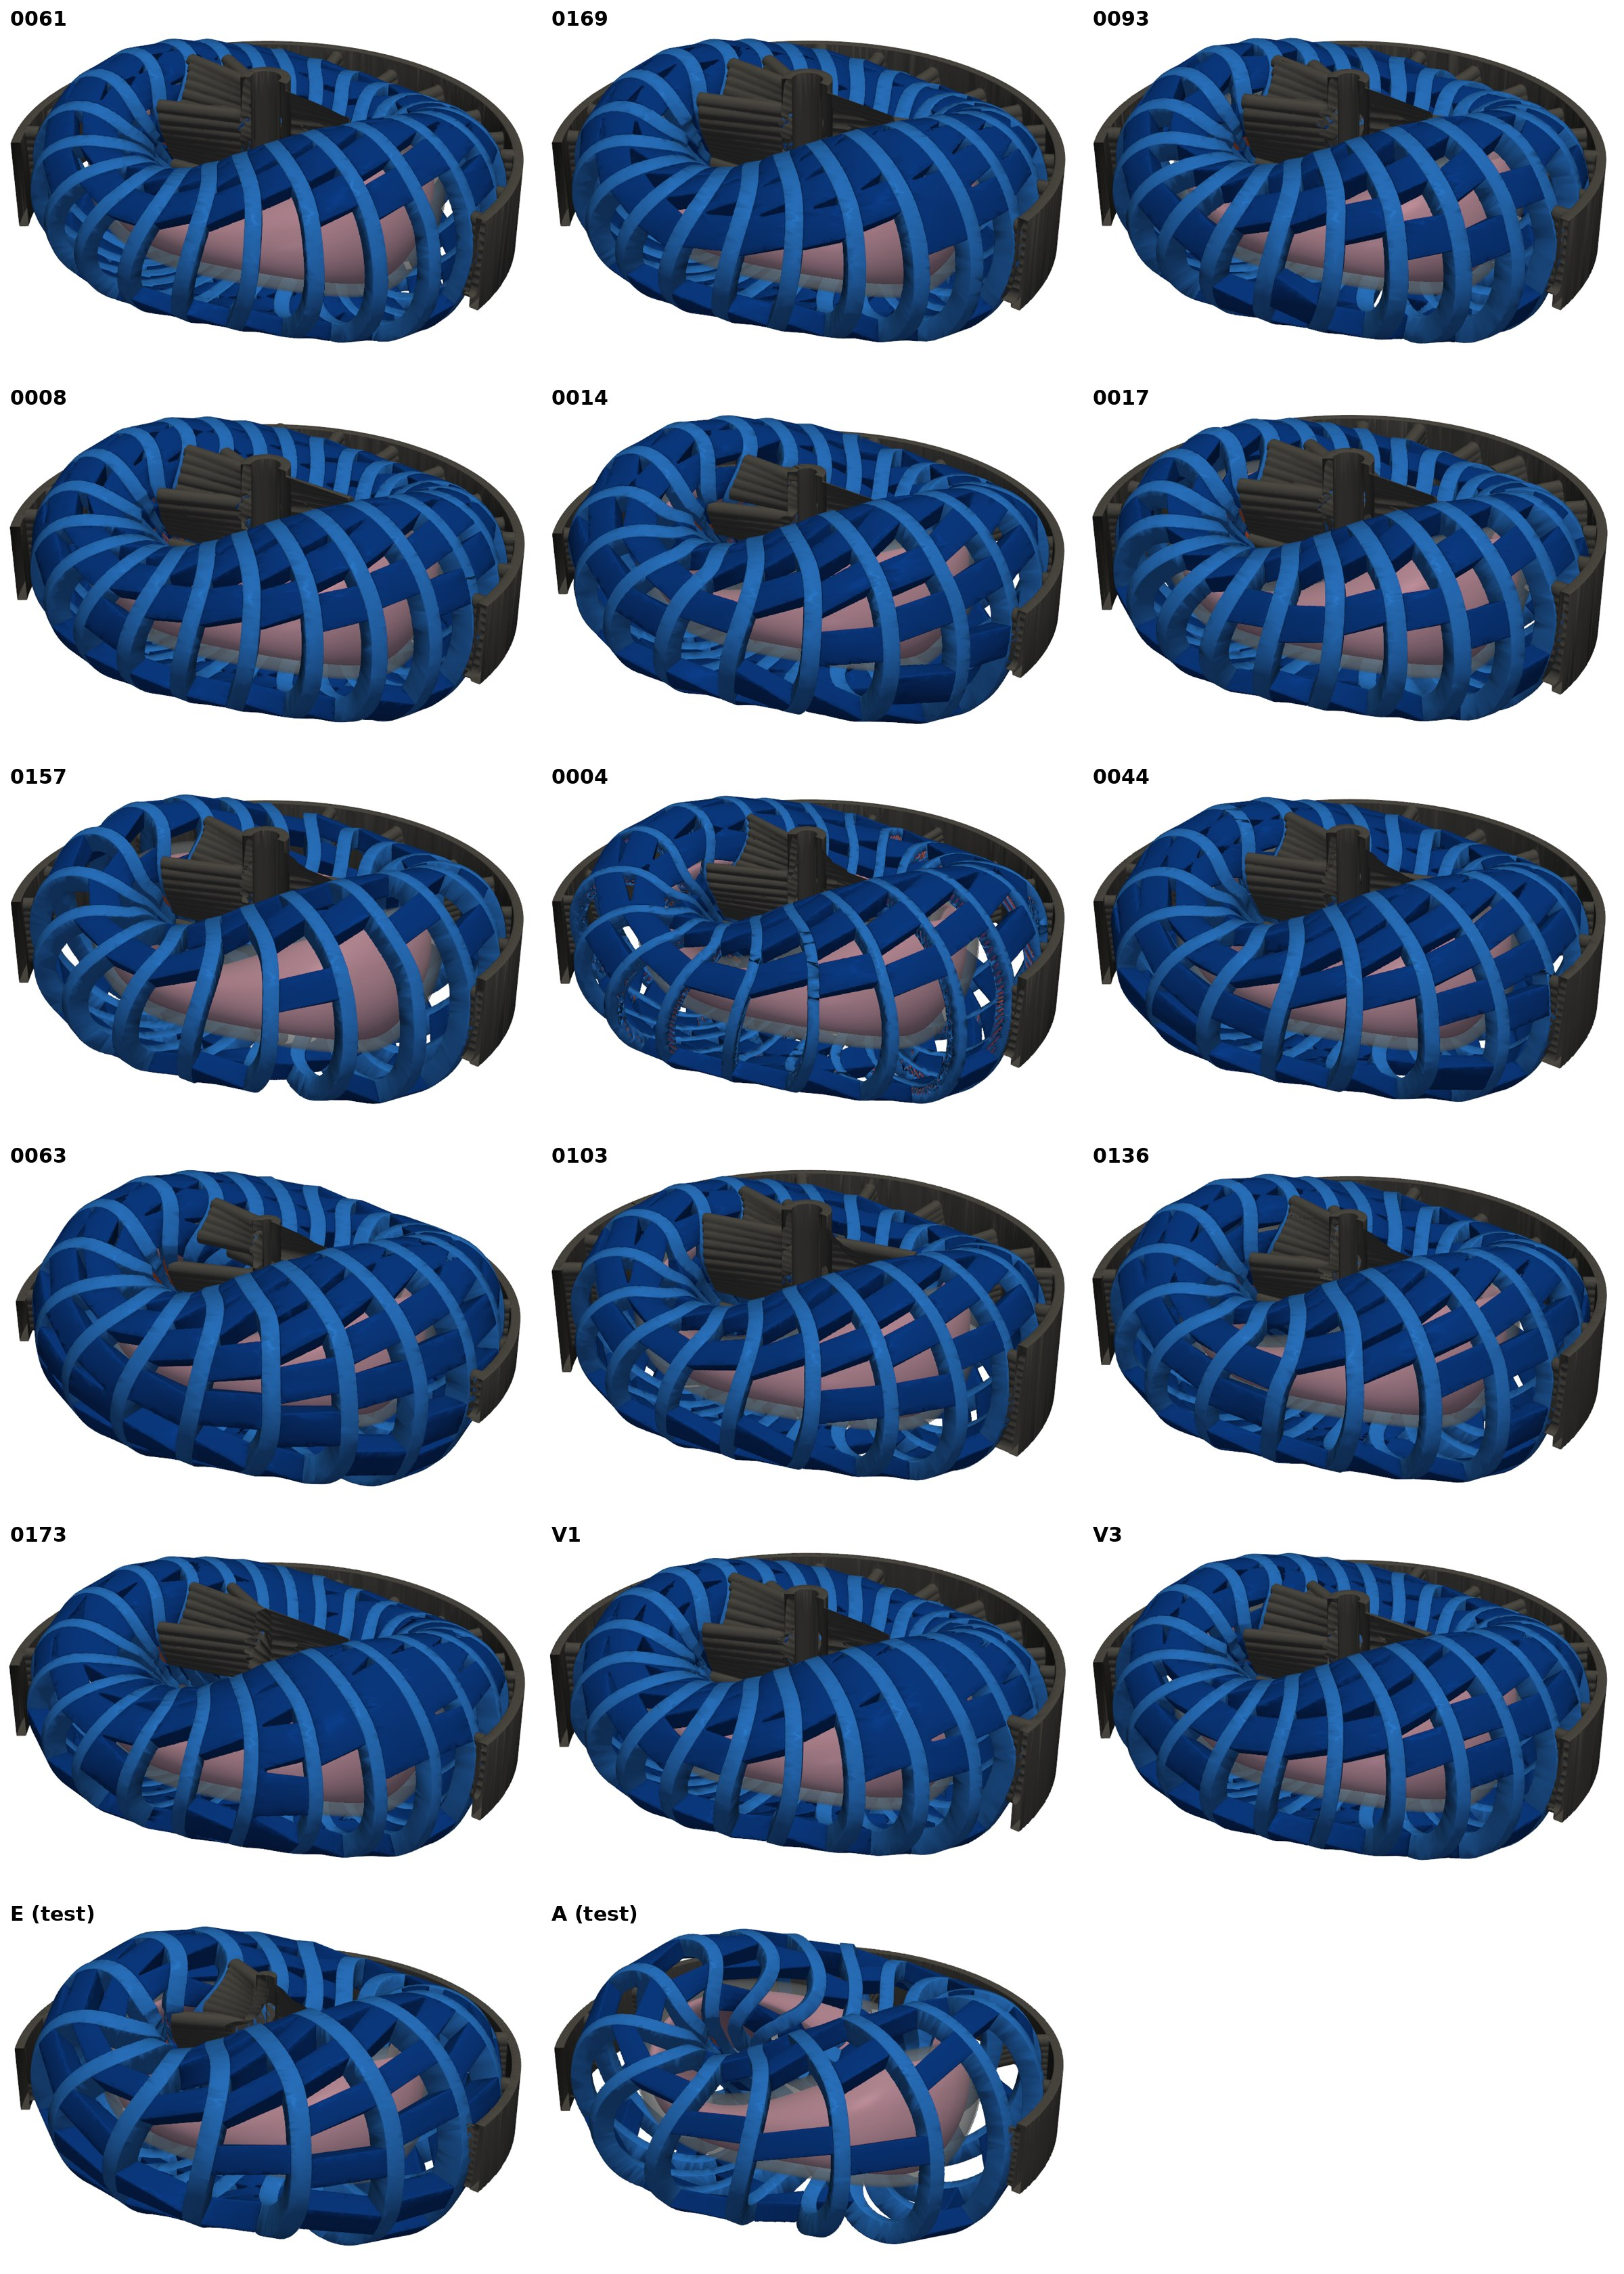
\includegraphics[width=\linewidth]{bilder/modell3d_montage_en.jpg}
\caption{All 3D models of the report (list 1) in overall view.}\end{figure}
\lesehilfe{Each panel is a complete PicoGK model, labelled with the design number. Blue are the coil cases, dark blue the
connectors, translucent grey the vacuum vessel, pink the plasma, dark grey the schematic bearings. Designs with 24 coils
look like a dense cage, the support tests A and E with 16 coils more open; in E the walls are visibly thicker.}

%======================================================================
\section{Data sheets of the designs in list~1}\label{sec:steckbriefe}
This section holds the data sheets of the seven admissible designs in list~1. The other entries of list~1 (those that
fail most narrowly, those that dropped out through the clean-up and the support tests A and E) no longer have a data
sheet of their own, so that the PDF file stays below 20~MB; their numbers remain in the tables and the catalogue.
Each data sheet shows design variables, results, the mesh study, the stress picture and
the PicoGK model in a stepped cut.
\lesehilfe{Stress picture: top view of all cases, colour from blue (\SI{0}{MPa}) via green and yellow to red
(\SI{800}{MPa} and more). Red spots at the sides of the cases are the connector joints. Stepped cut: each layer is cut
open at a different angle -- from inside to outside plasma (pink), first wall and blanket (yellow), shield (green),
vacuum vessel (grey), then the coils with their orange winding pack in cross-section.}


\clearpage
\subsection{Design 0061}\label{sb:0061}
\noindent\textbf{Verdict: }Admissible (cleaned), rank 1 of 7; smallest reserve 30 \% (σ99 steel 1.4429).\par\smallskip
\begin{minipage}[t]{0.46\linewidth}\small\begin{tabular}[t]{@{}lr@{}}\toprule\multicolumn{2}{@{}l}{\textbf{Design variables}}\\\midrule
coil–plasma distance & \num{0.204} \\
coils in total & 24 \\
coils per half period & \num{6} \\
length per coil & \num{4.58} \\
force weight & \num{0.010} \\
inner wall & \num{0.10} \\
side wall & \num{0.30} \\
outer wall min. & \num{0.52} \\
outer wall extra & \num{0.26} \\
connector stiffness & \num{93} \\
connectors per pair & \num{10} \\
bearing radius & \num{3.23} \\
\bottomrule\end{tabular}\end{minipage}\hfill
\begin{minipage}[t]{0.5\linewidth}\small\begin{tabular}[t]{@{}lr@{}}\toprule\multicolumn{2}{@{}l}{\textbf{Results}}\\\midrule
$\sigma_{99}$ steel 1.4429 & \num{351} MPa \\
largest element & \num{725} MPa \\
$P_m$ max. / 99 \% & \num{522} / \num{379} MPa \\
$P_m+P_b$ max. & \num{938} MPa \\
connectors σ99 & \num{191} MPa \\
max. deformation & \num{18} mm \\
winding-pack strain & \num{0.17} \% \\
current per coil & \num{14.7} MA \\
field at conductor & \num{15.6} T \\
utilisation / margin & \num{30} \% / \num{24} K \\
field error $B\cdot n$ & \num{1.49} ‰ \\
clearance plasma–case & \num{1.62} m \\
nuclear heating / fluence & \num{10} W/m³ / 8.0e16 \\
steel case + connectors & \num{9.5} + \num{9.9} kt \\
connectors built & 236 \\
\bottomrule\end{tabular}\end{minipage}\par\medskip
\noindent\textit{Mesh study ($\sigma_{99}$/max. in MPa): }doe1: 351/725; 1.5× stations: 556/6553; wall 3 cells: 346/861.\par\smallskip
\begin{figure}[H]\centering
\begin{minipage}[t]{0.49\linewidth}\centering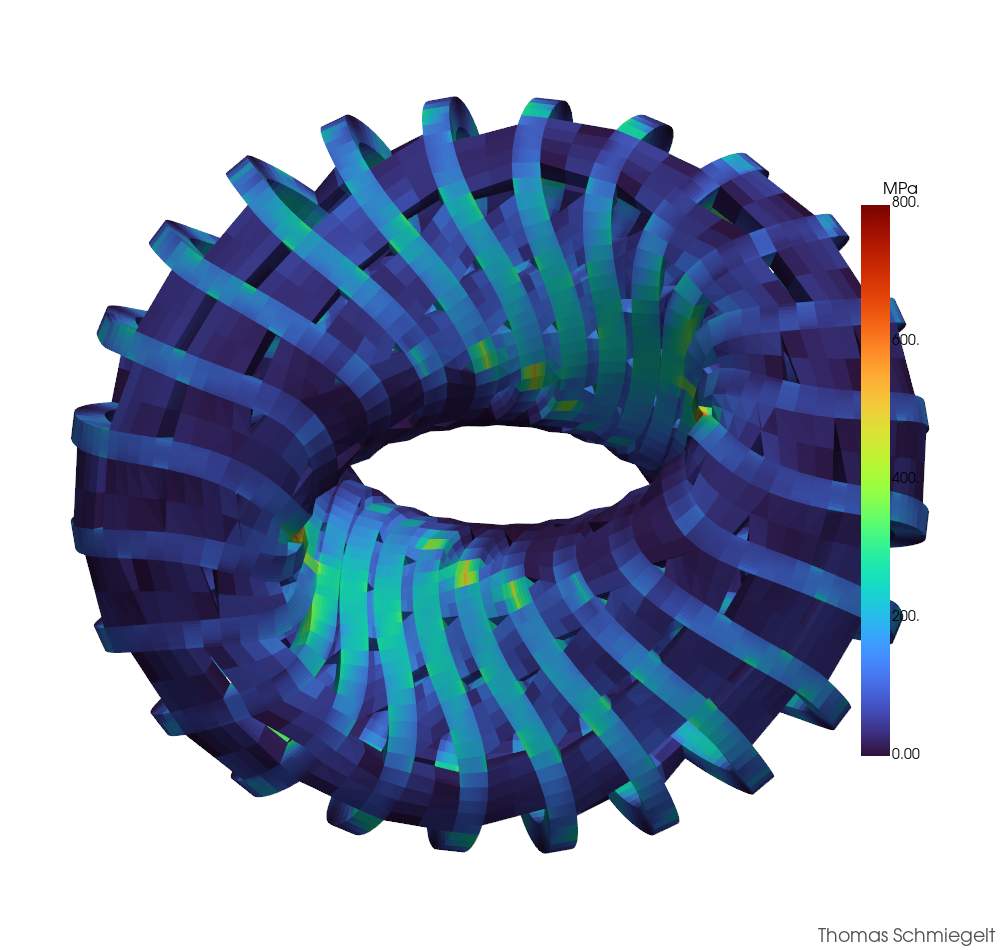
\includegraphics[width=\linewidth]{bilder/spannung_0061.png}\\\footnotesize von Mises stress in the steel (top view, 0–800 MPa)\end{minipage}\hfill
\begin{minipage}[t]{0.49\linewidth}\centering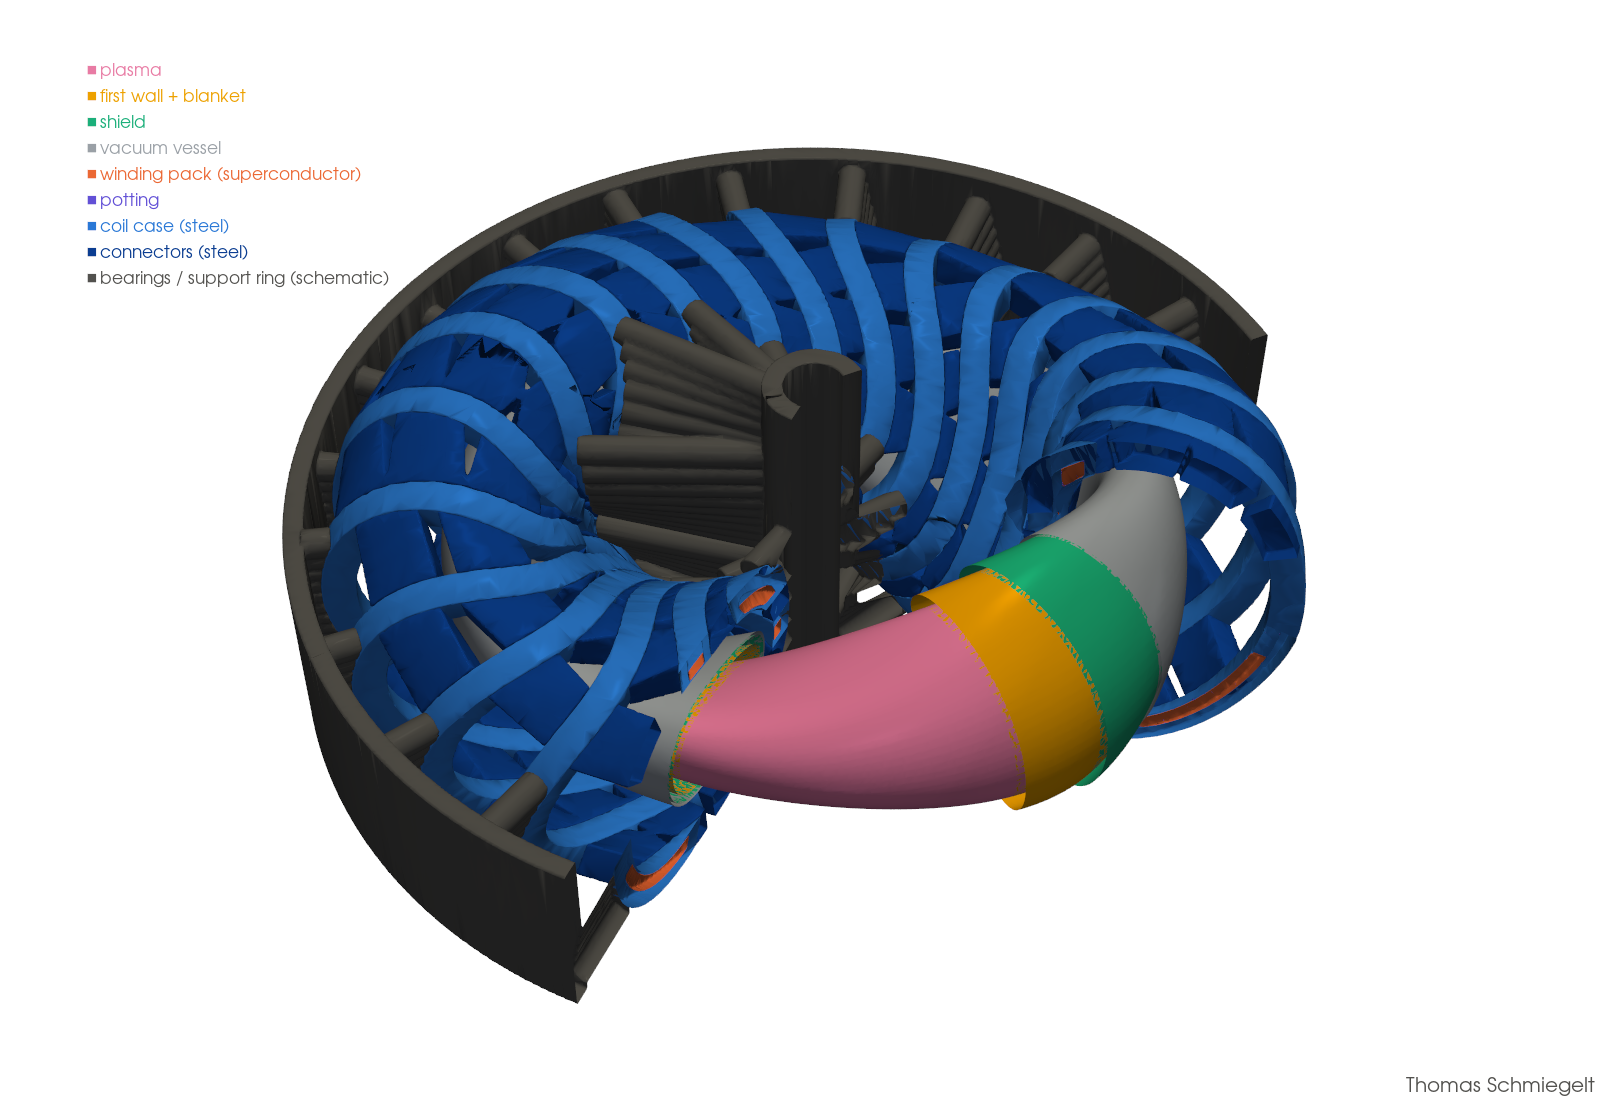
\includegraphics[width=\linewidth]{bilder/modell3d_0061_schnitt_en.png}\\\footnotesize PicoGK model, stepped cut\end{minipage}\hfill
\caption{Design 0061}\end{figure}
\clearpage
\subsection{Design 0169}\label{sb:0169}
\noindent\textbf{Verdict: }Admissible (cleaned), rank 2 of 7; smallest reserve 29 \% (package space).\par\smallskip
\begin{minipage}[t]{0.46\linewidth}\small\begin{tabular}[t]{@{}lr@{}}\toprule\multicolumn{2}{@{}l}{\textbf{Design variables}}\\\midrule
coil–plasma distance & \num{0.197} \\
coils in total & 24 \\
coils per half period & \num{6} \\
length per coil & \num{4.87} \\
force weight & \num{0.023} \\
inner wall & \num{0.27} \\
side wall & \num{0.34} \\
outer wall min. & \num{0.67} \\
outer wall extra & \num{0.25} \\
connector stiffness & \num{183} \\
connectors per pair & \num{13} \\
bearing radius & \num{3.29} \\
\bottomrule\end{tabular}\end{minipage}\hfill
\begin{minipage}[t]{0.5\linewidth}\small\begin{tabular}[t]{@{}lr@{}}\toprule\multicolumn{2}{@{}l}{\textbf{Results}}\\\midrule
$\sigma_{99}$ steel 1.4429 & \num{308} MPa \\
largest element & \num{717} MPa \\
$P_m$ max. / 99 \% & \num{626} / \num{333} MPa \\
$P_m+P_b$ max. & \num{817} MPa \\
connectors σ99 & \num{192} MPa \\
max. deformation & \num{19} mm \\
winding-pack strain & \num{0.15} \% \\
current per coil & \num{14.7} MA \\
field at conductor & \num{15.5} T \\
utilisation / margin & \num{30} \% / \num{24} K \\
field error $B\cdot n$ & \num{2.13} ‰ \\
clearance plasma–case & \num{1.39} m \\
nuclear heating / fluence & \num{103} W/m³ / 8.5e17 \\
steel case + connectors & \num{12.8} + \num{15.2} kt \\
connectors built & 292 \\
\bottomrule\end{tabular}\end{minipage}\par\medskip
\noindent\textit{Mesh study ($\sigma_{99}$/max. in MPa): }doe1: 219/421; standard: 308/717; 1.5× stations: 319/1262; wall 3 cells: 308/794.\par\smallskip
\begin{figure}[H]\centering
\begin{minipage}[t]{0.49\linewidth}\centering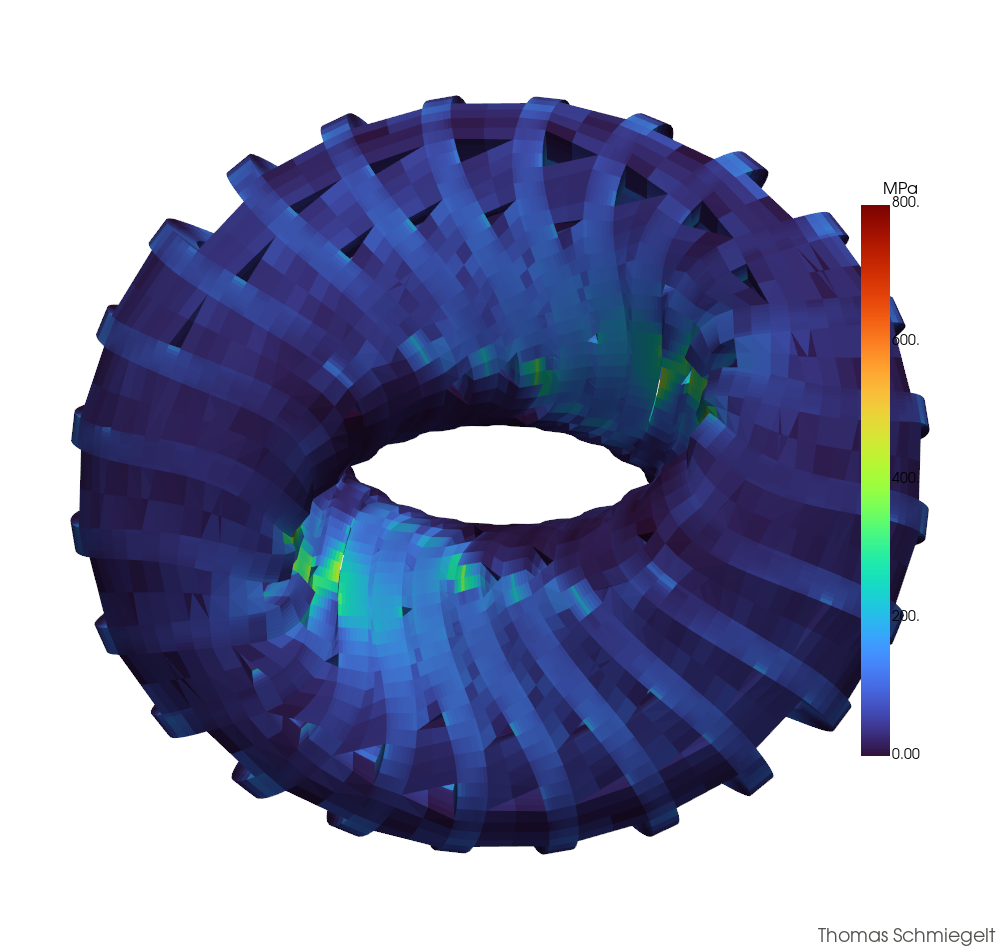
\includegraphics[width=\linewidth]{bilder/spannung_0169.png}\\\footnotesize von Mises stress in the steel (top view, 0–800 MPa)\end{minipage}\hfill
\begin{minipage}[t]{0.49\linewidth}\centering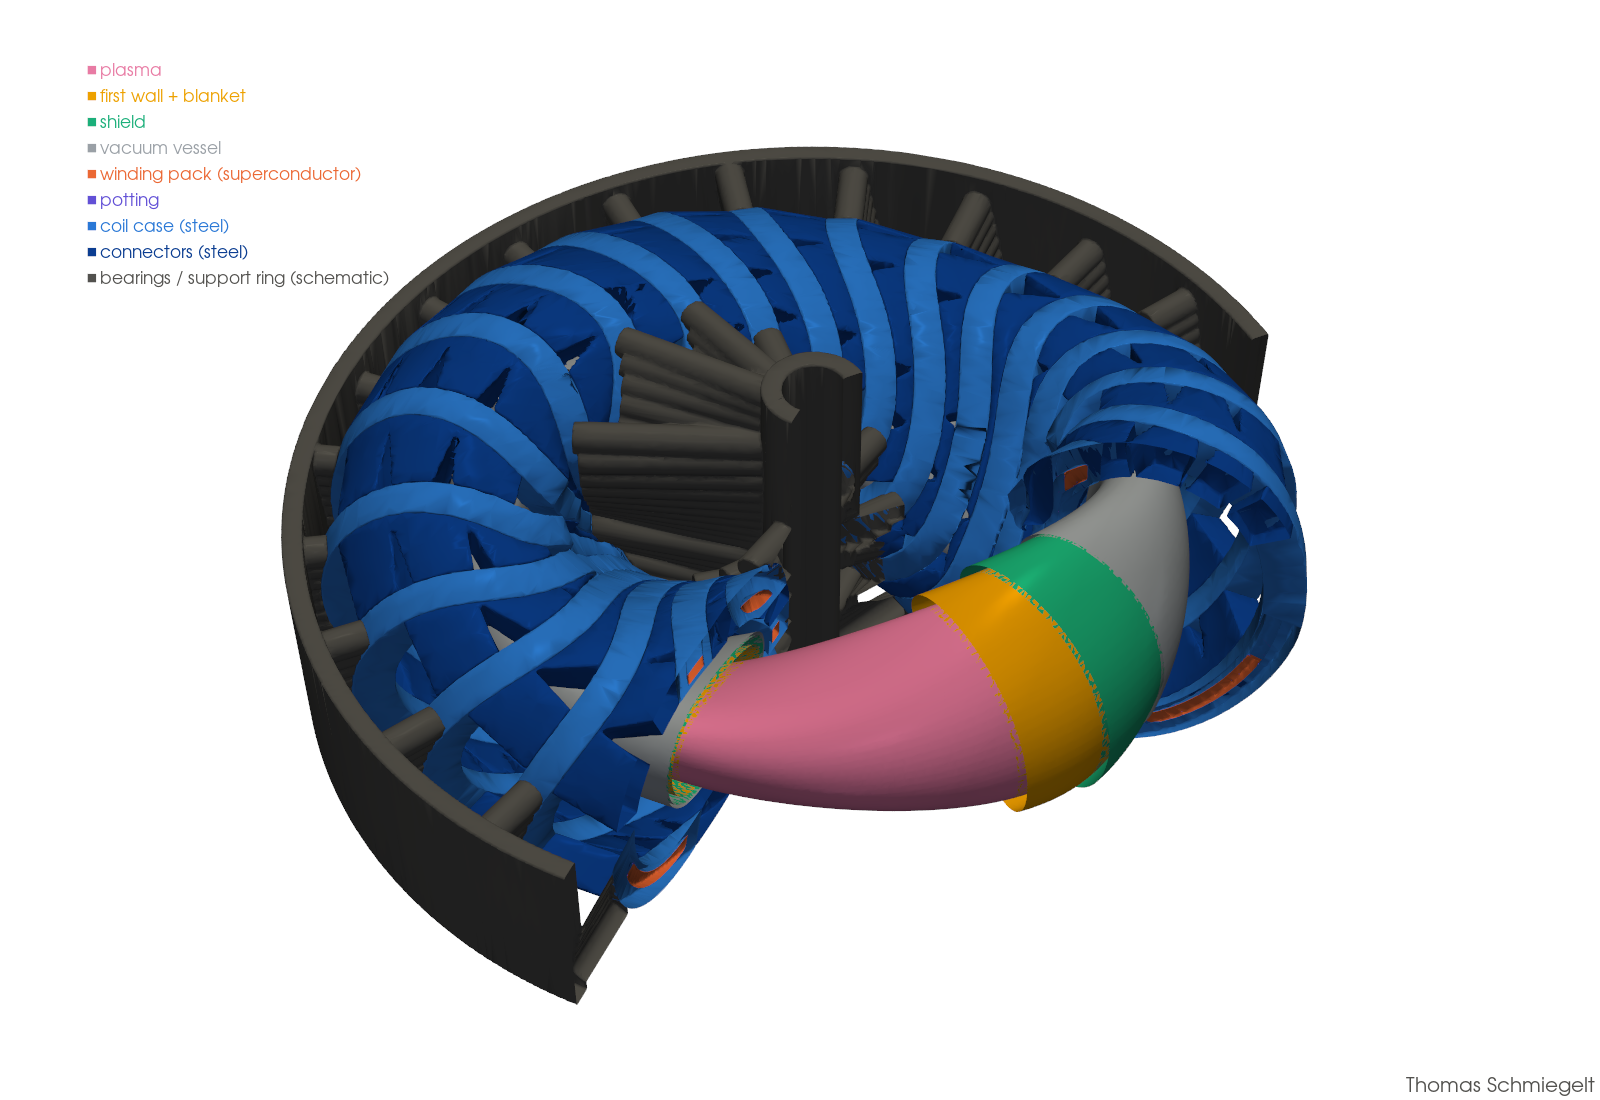
\includegraphics[width=\linewidth]{bilder/modell3d_0169_schnitt_en.png}\\\footnotesize PicoGK model, stepped cut\end{minipage}\hfill
\caption{Design 0169}\end{figure}
\clearpage
\subsection{Design 0093}\label{sb:0093}
\noindent\textbf{Verdict: }Admissible (cleaned), rank 3 of 7; smallest reserve 27 \% (package space).\par\smallskip
\begin{minipage}[t]{0.46\linewidth}\small\begin{tabular}[t]{@{}lr@{}}\toprule\multicolumn{2}{@{}l}{\textbf{Design variables}}\\\midrule
coil–plasma distance & \num{0.206} \\
coils in total & 24 \\
coils per half period & \num{6} \\
length per coil & \num{4.14} \\
force weight & \num{0.010} \\
inner wall & \num{0.38} \\
side wall & \num{0.38} \\
outer wall min. & \num{0.73} \\
outer wall extra & \num{0.38} \\
connector stiffness & \num{64} \\
connectors per pair & \num{8} \\
bearing radius & \num{3.49} \\
\bottomrule\end{tabular}\end{minipage}\hfill
\begin{minipage}[t]{0.5\linewidth}\small\begin{tabular}[t]{@{}lr@{}}\toprule\multicolumn{2}{@{}l}{\textbf{Results}}\\\midrule
$\sigma_{99}$ steel 1.4429 & \num{283} MPa \\
largest element & \num{1190} MPa \\
$P_m$ max. / 99 \% & \num{1147} / \num{340} MPa \\
$P_m+P_b$ max. & \num{1233} MPa \\
connectors σ99 & \num{154} MPa \\
max. deformation & \num{20} mm \\
winding-pack strain & \num{0.16} \% \\
current per coil & \num{14.7} MA \\
field at conductor & \num{15.7} T \\
utilisation / margin & \num{30} \% / \num{24} K \\
field error $B\cdot n$ & \num{1.45} ‰ \\
clearance plasma–case & \num{1.37} m \\
nuclear heating / fluence & \num{117} W/m³ / 9.8e17 \\
steel case + connectors & \num{16.5} + \num{11.6} kt \\
connectors built & 190 \\
\bottomrule\end{tabular}\end{minipage}\par\medskip
\noindent\textit{Mesh study ($\sigma_{99}$/max. in MPa): }doe1: 283/1190; 1.5× stations: 410/2343; wall 3 cells: 280/1432.\par\smallskip
\begin{figure}[H]\centering
\begin{minipage}[t]{0.49\linewidth}\centering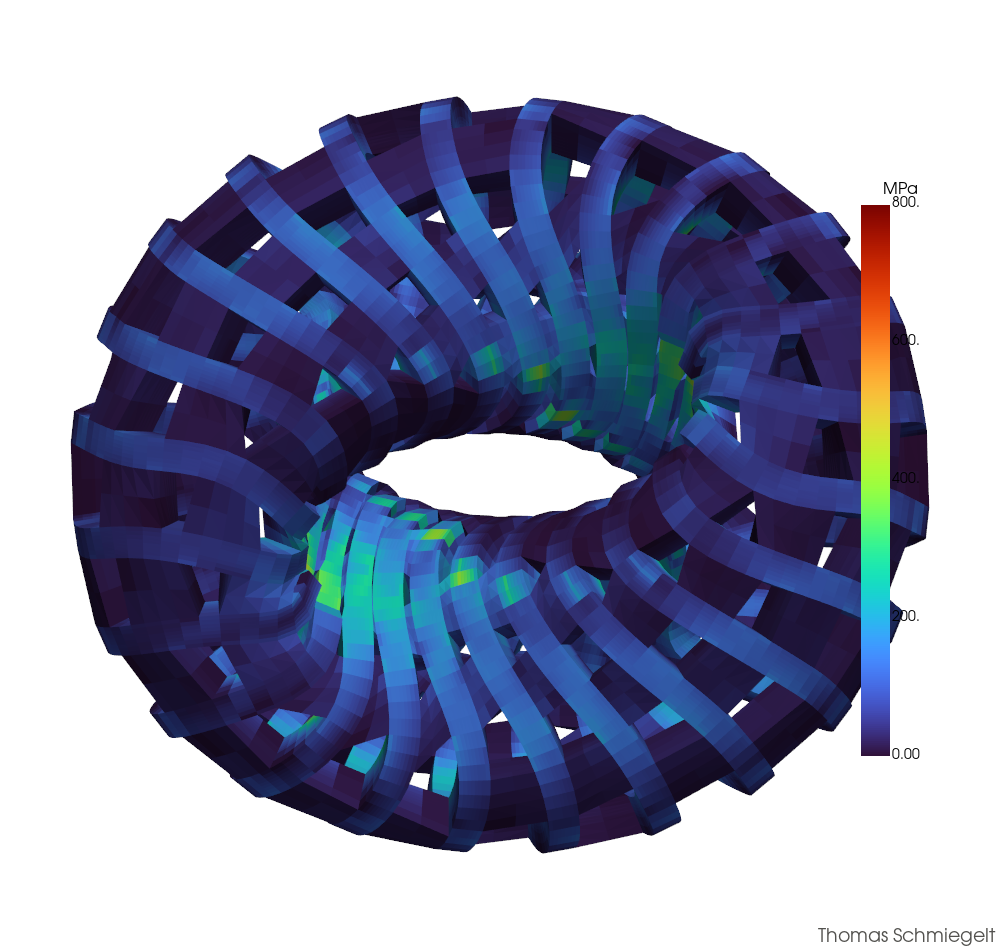
\includegraphics[width=\linewidth]{bilder/spannung_0093.png}\\\footnotesize von Mises stress in the steel (top view, 0–800 MPa)\end{minipage}\hfill
\begin{minipage}[t]{0.49\linewidth}\centering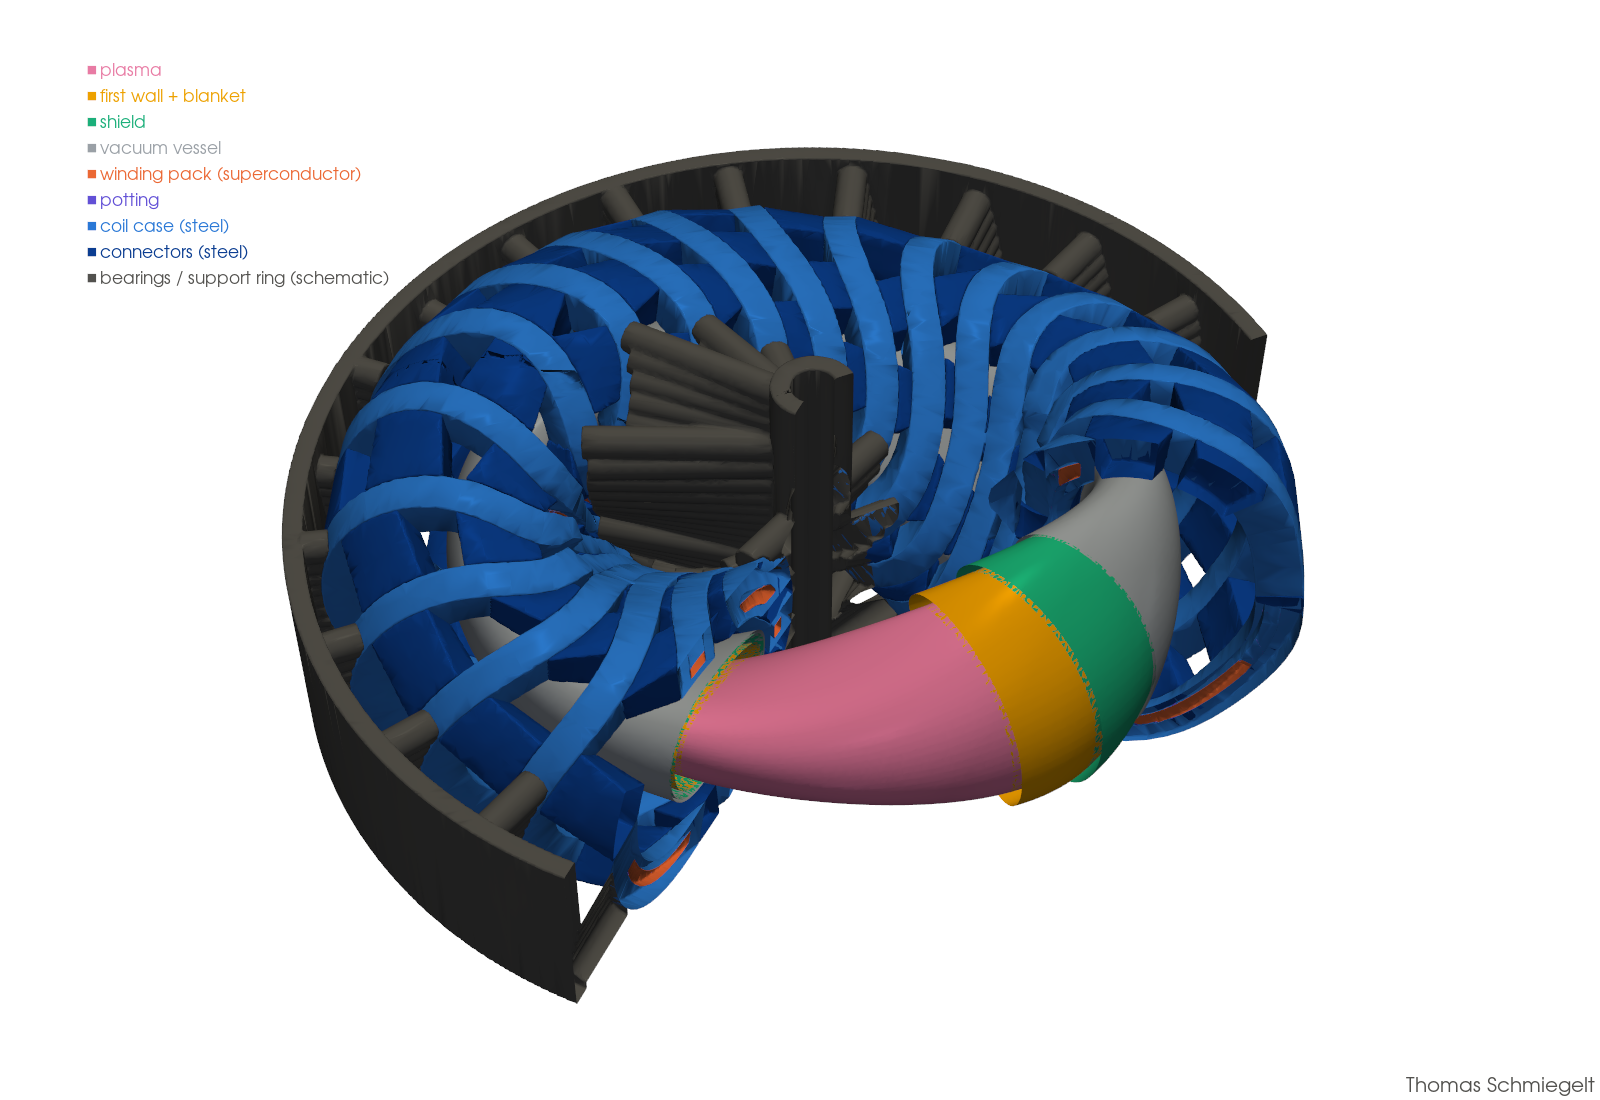
\includegraphics[width=\linewidth]{bilder/modell3d_0093_schnitt_en.png}\\\footnotesize PicoGK model, stepped cut\end{minipage}\hfill
\caption{Design 0093}\end{figure}
\clearpage
\subsection{Design 0008}\label{sb:0008}
\noindent\textbf{Verdict: }Admissible (cleaned), rank 4 of 7; smallest reserve 27 \% (field error B·n).\par\smallskip
\begin{minipage}[t]{0.46\linewidth}\small\begin{tabular}[t]{@{}lr@{}}\toprule\multicolumn{2}{@{}l}{\textbf{Design variables}}\\\midrule
coil–plasma distance & \num{0.211} \\
coils in total & 24 \\
coils per half period & \num{6} \\
length per coil & \num{3.66} \\
force weight & \num{0.030} \\
inner wall & \num{0.32} \\
side wall & \num{0.31} \\
outer wall min. & \num{0.72} \\
outer wall extra & \num{0.17} \\
connector stiffness & \num{142} \\
connectors per pair & \num{11} \\
bearing radius & \num{2.80} \\
\bottomrule\end{tabular}\end{minipage}\hfill
\begin{minipage}[t]{0.5\linewidth}\small\begin{tabular}[t]{@{}lr@{}}\toprule\multicolumn{2}{@{}l}{\textbf{Results}}\\\midrule
$\sigma_{99}$ steel 1.4429 & \num{305} MPa \\
largest element & \num{1695} MPa \\
$P_m$ max. / 99 \% & \num{1687} / \num{344} MPa \\
$P_m+P_b$ max. & \num{1704} MPa \\
connectors σ99 & \num{187} MPa \\
max. deformation & \num{19} mm \\
winding-pack strain & \num{0.17} \% \\
current per coil & \num{14.7} MA \\
field at conductor & \num{15.7} T \\
utilisation / margin & \num{30} \% / \num{24} K \\
field error $B\cdot n$ & \num{2.20} ‰ \\
clearance plasma–case & \num{1.48} m \\
nuclear heating / fluence & \num{40} W/m³ / 3.3e17 \\
steel case + connectors & \num{12.2} + \num{13.7} kt \\
connectors built & 252 \\
\bottomrule\end{tabular}\end{minipage}\par\medskip
\noindent\textit{Mesh study ($\sigma_{99}$/max. in MPa): }doe1: 305/1695; 1.5× stations: 407/3250; wall 3 cells: 306/1931.\par\smallskip
\begin{figure}[H]\centering
\begin{minipage}[t]{0.49\linewidth}\centering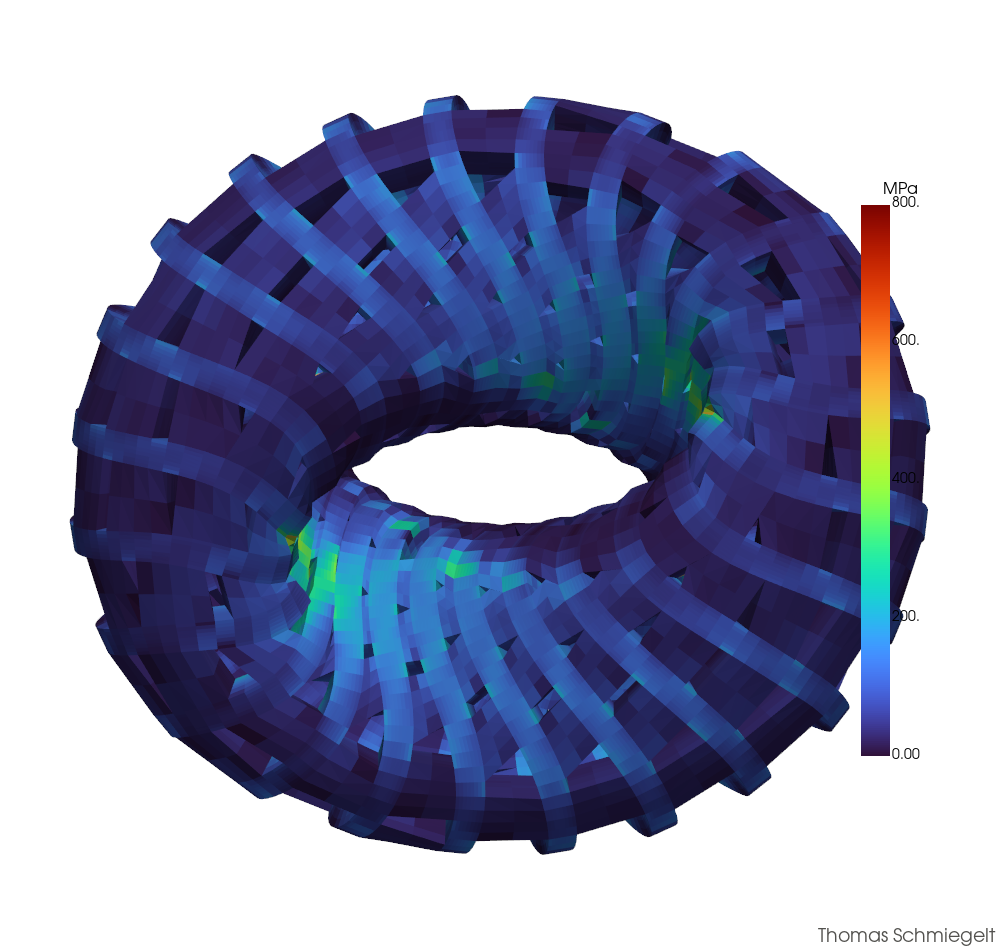
\includegraphics[width=\linewidth]{bilder/spannung_0008.png}\\\footnotesize von Mises stress in the steel (top view, 0–800 MPa)\end{minipage}\hfill
\begin{minipage}[t]{0.49\linewidth}\centering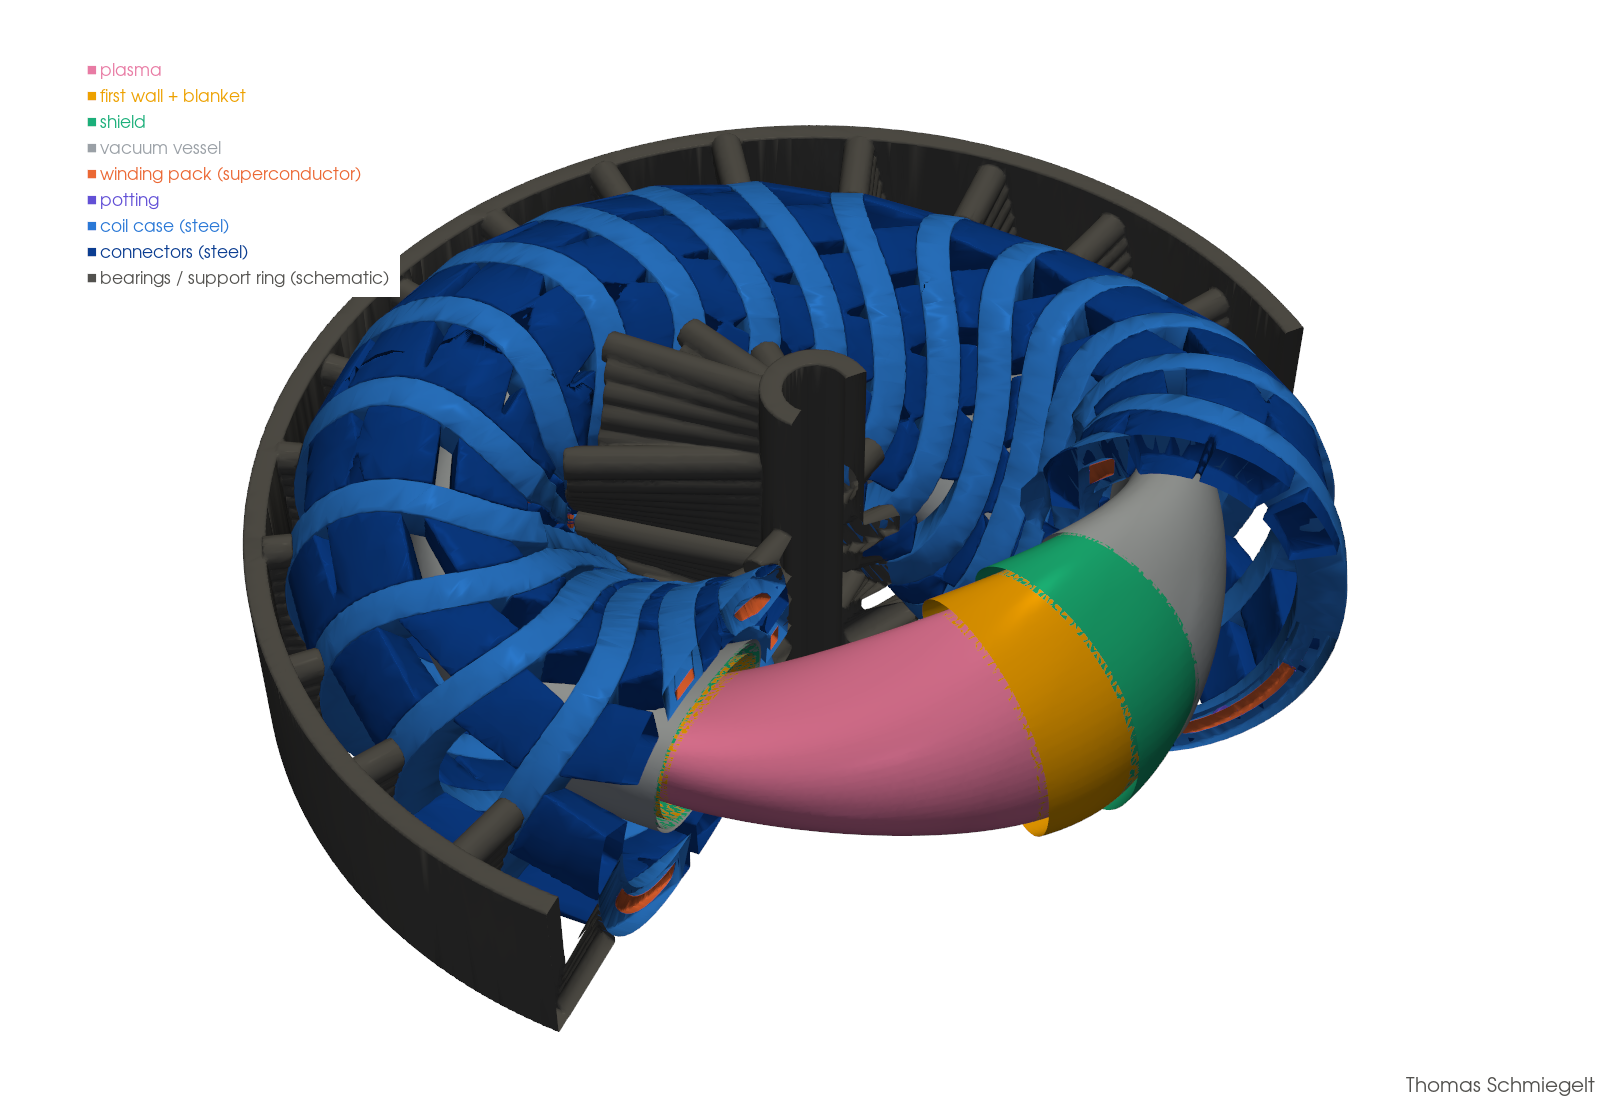
\includegraphics[width=\linewidth]{bilder/modell3d_0008_schnitt_en.png}\\\footnotesize PicoGK model, stepped cut\end{minipage}\hfill
\caption{Design 0008}\end{figure}
\clearpage
\subsection{Design 0014}\label{sb:0014}
\noindent\textbf{Verdict: }Admissible (cleaned), rank 5 of 7; smallest reserve 25 \% (σ99 steel 1.4429).\par\smallskip
\begin{minipage}[t]{0.46\linewidth}\small\begin{tabular}[t]{@{}lr@{}}\toprule\multicolumn{2}{@{}l}{\textbf{Design variables}}\\\midrule
coil–plasma distance & \num{0.233} \\
coils in total & 20 \\
coils per half period & \num{5} \\
length per coil & \num{4.34} \\
force weight & \num{0.025} \\
inner wall & \num{0.35} \\
side wall & \num{0.32} \\
outer wall min. & \num{0.63} \\
outer wall extra & \num{0.29} \\
connector stiffness & \num{196} \\
connectors per pair & \num{11} \\
bearing radius & \num{2.04} \\
\bottomrule\end{tabular}\end{minipage}\hfill
\begin{minipage}[t]{0.5\linewidth}\small\begin{tabular}[t]{@{}lr@{}}\toprule\multicolumn{2}{@{}l}{\textbf{Results}}\\\midrule
$\sigma_{99}$ steel 1.4429 & \num{377} MPa \\
largest element & \num{1419} MPa \\
$P_m$ max. / 99 \% & \num{1369} / \num{459} MPa \\
$P_m+P_b$ max. & \num{1491} MPa \\
connectors σ99 & \num{243} MPa \\
max. deformation & \num{18} mm \\
winding-pack strain & \num{0.21} \% \\
current per coil & \num{17.7} MA \\
field at conductor & \num{16.9} T \\
utilisation / margin & \num{32} \% / \num{23} K \\
field error $B\cdot n$ & \num{2.21} ‰ \\
clearance plasma–case & \num{1.65} m \\
nuclear heating / fluence & \num{8} W/m³ / 6.5e16 \\
steel case + connectors & \num{12.5} + \num{15.5} kt \\
connectors built & 212 \\
\bottomrule\end{tabular}\end{minipage}\par\medskip
\noindent\textit{Mesh study ($\sigma_{99}$/max. in MPa): }doe1: 377/1419; 1.5× stations: 549/3814; wall 3 cells: 375/1639.\par\smallskip
\begin{figure}[H]\centering
\begin{minipage}[t]{0.49\linewidth}\centering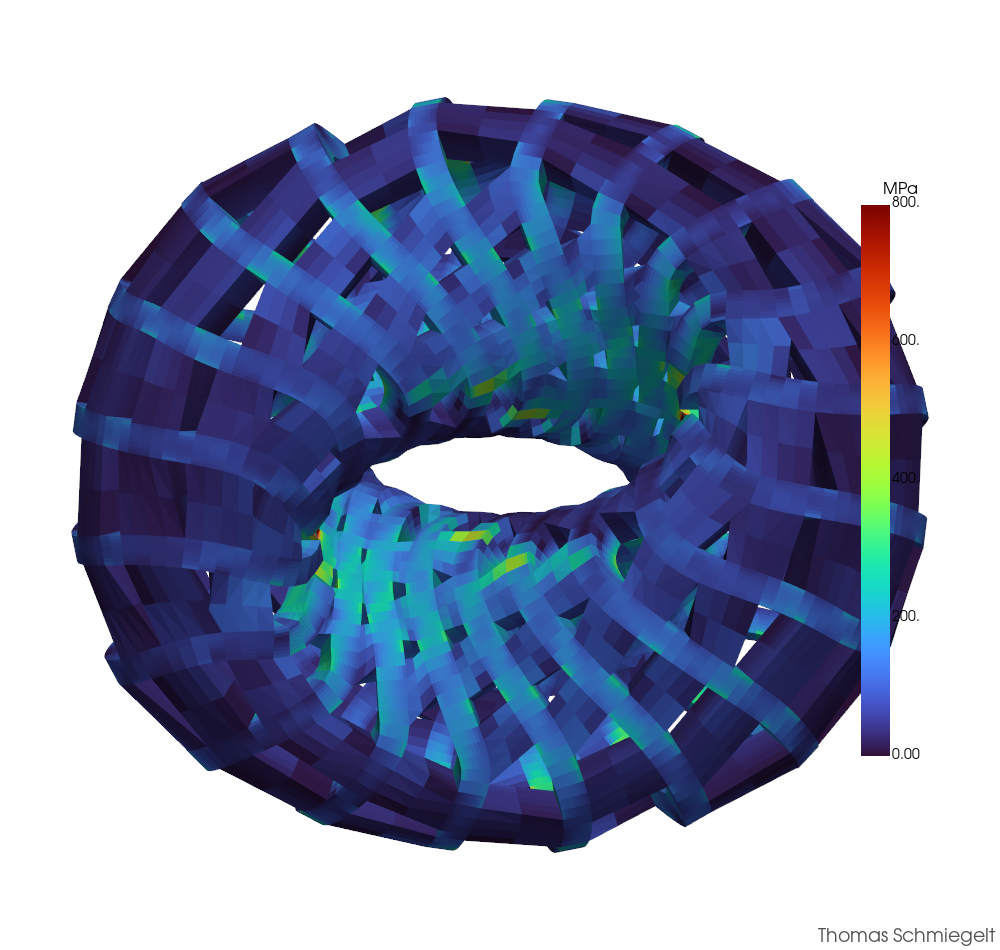
\includegraphics[width=\linewidth]{bilder/spannung_0014.png}\\\footnotesize von Mises stress in the steel (top view, 0–800 MPa)\end{minipage}\hfill
\begin{minipage}[t]{0.49\linewidth}\centering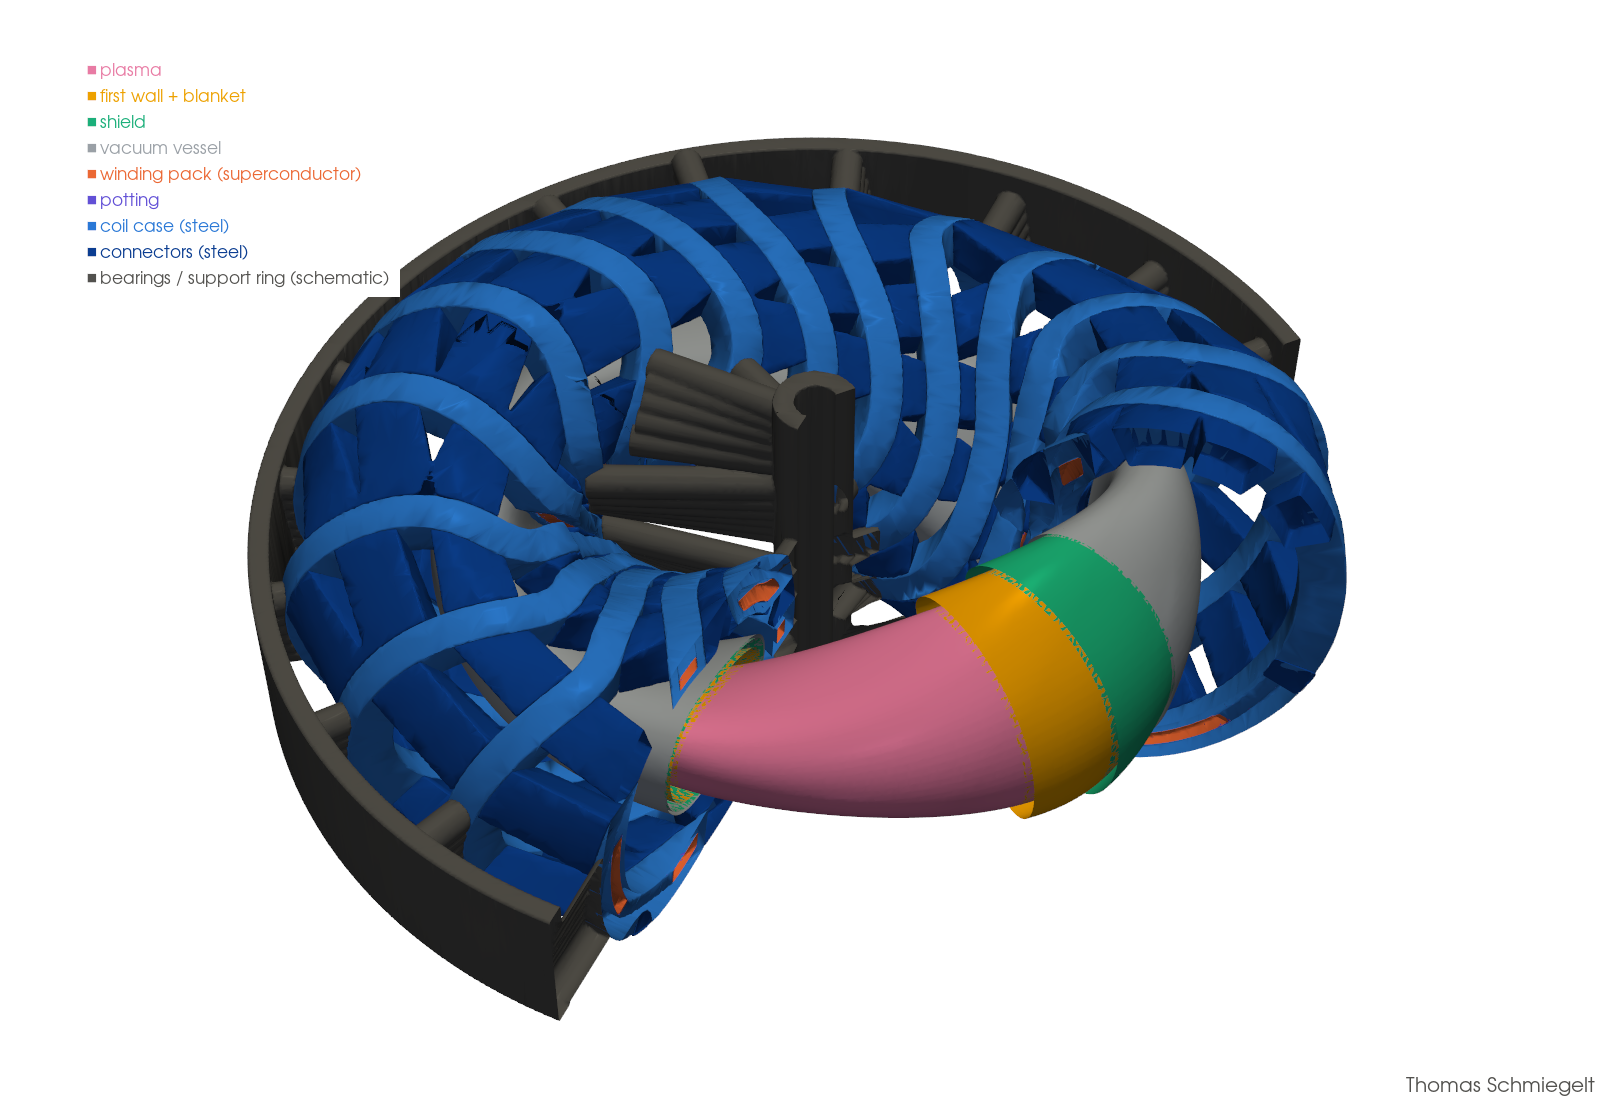
\includegraphics[width=\linewidth]{bilder/modell3d_0014_schnitt_en.png}\\\footnotesize PicoGK model, stepped cut\end{minipage}\hfill
\caption{Design 0014}\end{figure}
\clearpage
\subsection{Design 0017}\label{sb:0017}
\noindent\textbf{Verdict: }Admissible (cleaned), rank 6 of 7; smallest reserve 20 \% (package space).\par\smallskip
\begin{minipage}[t]{0.46\linewidth}\small\begin{tabular}[t]{@{}lr@{}}\toprule\multicolumn{2}{@{}l}{\textbf{Design variables}}\\\midrule
coil–plasma distance & \num{0.220} \\
coils in total & 24 \\
coils per half period & \num{6} \\
length per coil & \num{3.77} \\
force weight & \num{0.019} \\
inner wall & \num{0.60} \\
side wall & \num{0.37} \\
outer wall min. & \num{0.43} \\
outer wall extra & \num{0.32} \\
connector stiffness & \num{29} \\
connectors per pair & \num{7} \\
bearing radius & \num{3.47} \\
\bottomrule\end{tabular}\end{minipage}\hfill
\begin{minipage}[t]{0.5\linewidth}\small\begin{tabular}[t]{@{}lr@{}}\toprule\multicolumn{2}{@{}l}{\textbf{Results}}\\\midrule
$\sigma_{99}$ steel 1.4429 & \num{389} MPa \\
largest element & \num{1721} MPa \\
$P_m$ max. / 99 \% & \num{1631} / \num{448} MPa \\
$P_m+P_b$ max. & \num{1813} MPa \\
connectors σ99 & \num{131} MPa \\
max. deformation & \num{31} mm \\
winding-pack strain & \num{0.20} \% \\
current per coil & \num{14.7} MA \\
field at conductor & \num{16.0} T \\
utilisation / margin & \num{30} \% / \num{24} K \\
field error $B\cdot n$ & \num{1.66} ‰ \\
clearance plasma–case & \num{1.30} m \\
nuclear heating / fluence & \num{245} W/m³ / 2.0e18 \\
steel case + connectors & \num{13.9} + \num{8.7} kt \\
connectors built & 162 \\
\bottomrule\end{tabular}\end{minipage}\par\medskip
\begin{figure}[H]\centering
\begin{minipage}[t]{0.49\linewidth}\centering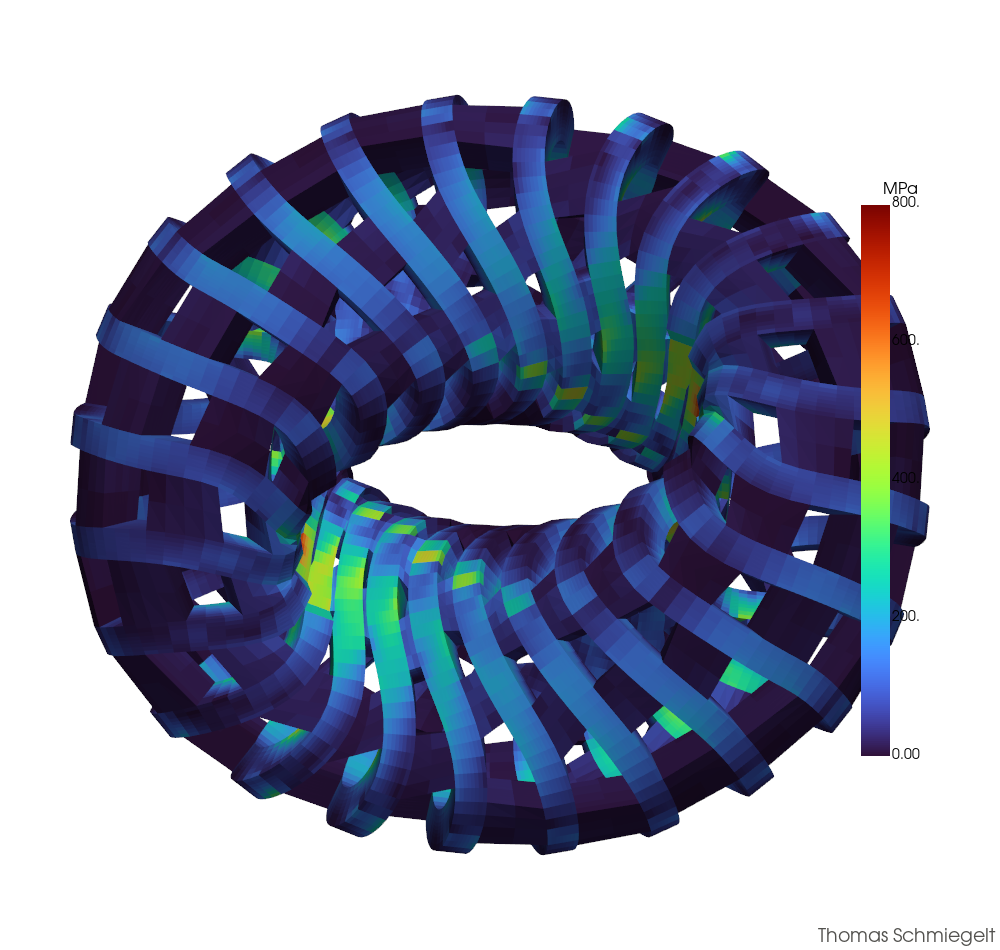
\includegraphics[width=\linewidth]{bilder/spannung_0017.png}\\\footnotesize von Mises stress in the steel (top view, 0–800 MPa)\end{minipage}\hfill
\begin{minipage}[t]{0.49\linewidth}\centering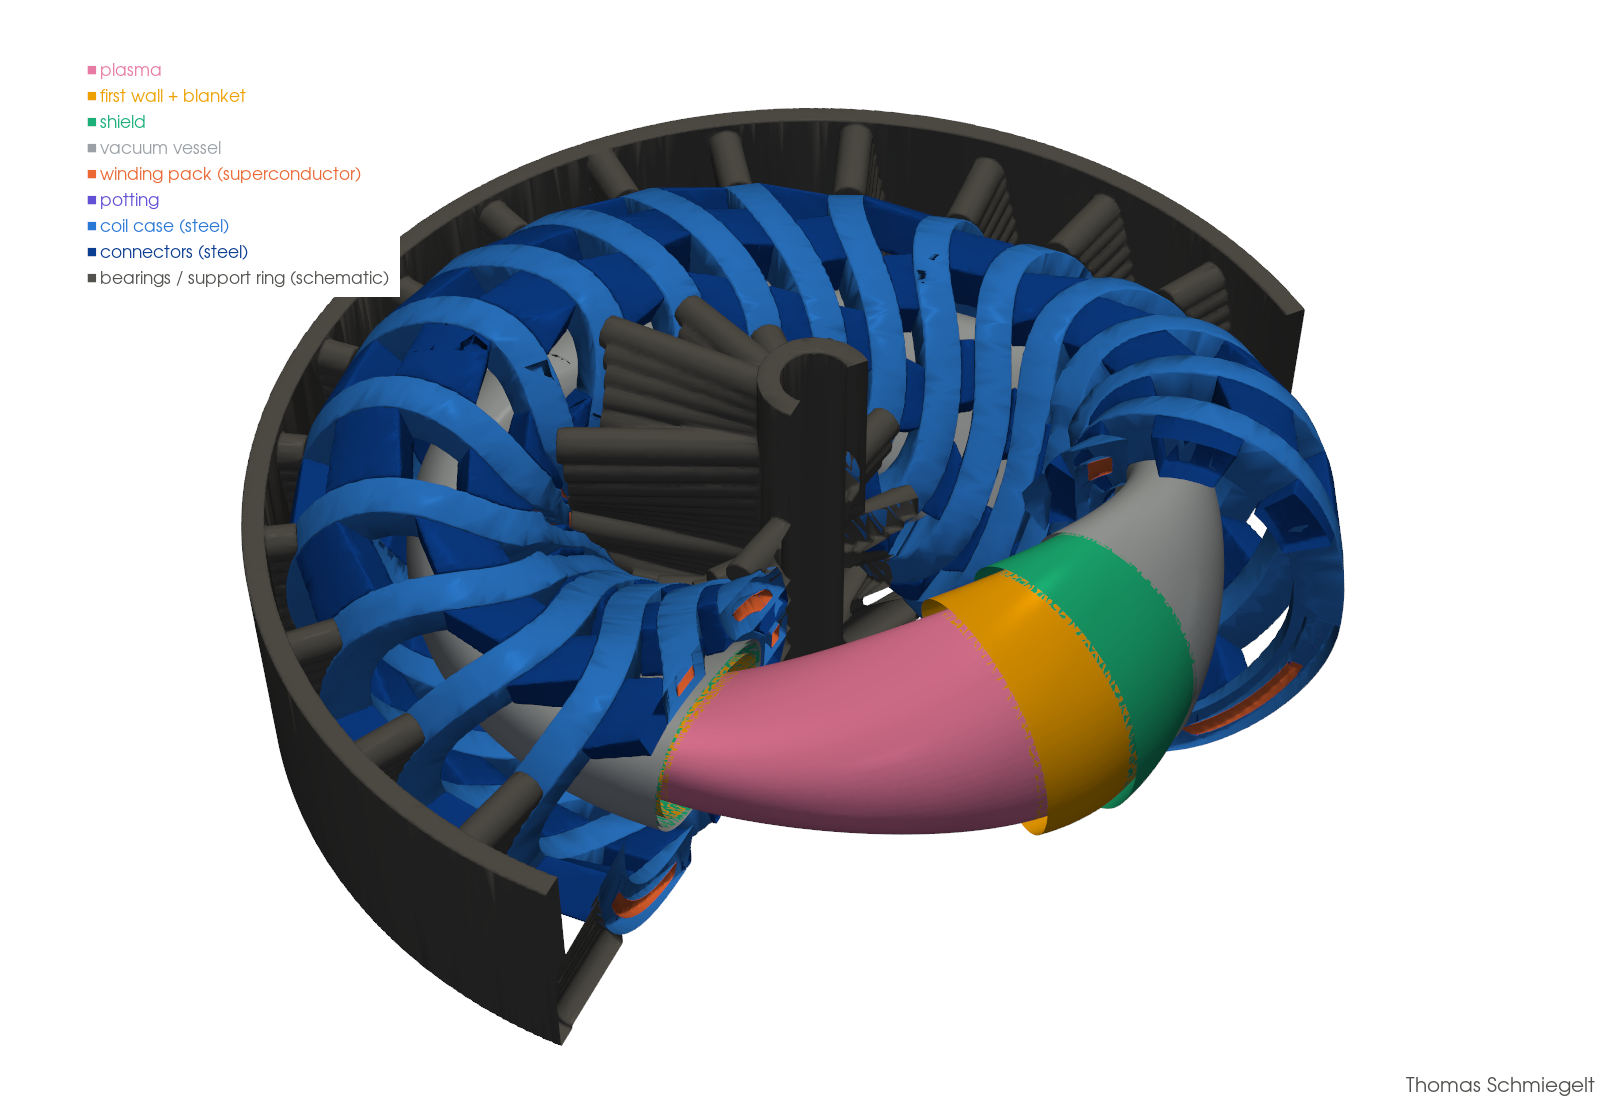
\includegraphics[width=\linewidth]{bilder/modell3d_0017_schnitt_en.png}\\\footnotesize PicoGK model, stepped cut\end{minipage}\hfill
\caption{Design 0017}\end{figure}
\clearpage
\subsection{Design 0157}\label{sb:0157}
\noindent\textbf{Verdict: }Admissible (cleaned), rank 7 of 7; smallest reserve 2 \% (σ99 steel 1.4429).\par\smallskip
\begin{minipage}[t]{0.46\linewidth}\small\begin{tabular}[t]{@{}lr@{}}\toprule\multicolumn{2}{@{}l}{\textbf{Design variables}}\\\midrule
coil–plasma distance & \num{0.218} \\
coils in total & 20 \\
coils per half period & \num{5} \\
length per coil & \num{4.09} \\
force weight & \num{0.020} \\
inner wall & \num{0.49} \\
side wall & \num{0.25} \\
outer wall min. & \num{0.58} \\
outer wall extra & \num{0.02} \\
connector stiffness & \num{158} \\
connectors per pair & \num{6} \\
bearing radius & \num{3.06} \\
\bottomrule\end{tabular}\end{minipage}\hfill
\begin{minipage}[t]{0.5\linewidth}\small\begin{tabular}[t]{@{}lr@{}}\toprule\multicolumn{2}{@{}l}{\textbf{Results}}\\\midrule
$\sigma_{99}$ steel 1.4429 & \num{492} MPa \\
largest element & \num{1658} MPa \\
$P_m$ max. / 99 \% & \num{1405} / \num{519} MPa \\
$P_m+P_b$ max. & \num{1920} MPa \\
connectors σ99 & \num{335} MPa \\
max. deformation & \num{34} mm \\
winding-pack strain & \num{0.22} \% \\
current per coil & \num{17.7} MA \\
field at conductor & \num{16.5} T \\
utilisation / margin & \num{31} \% / \num{23} K \\
field error $B\cdot n$ & \num{2.37} ‰ \\
clearance plasma–case & \num{1.35} m \\
nuclear heating / fluence & \num{142} W/m³ / 1.2e18 \\
steel case + connectors & \num{10.1} + \num{7.5} kt \\
connectors built & 118 \\
\bottomrule\end{tabular}\end{minipage}\par\medskip
\begin{figure}[H]\centering
\begin{minipage}[t]{0.49\linewidth}\centering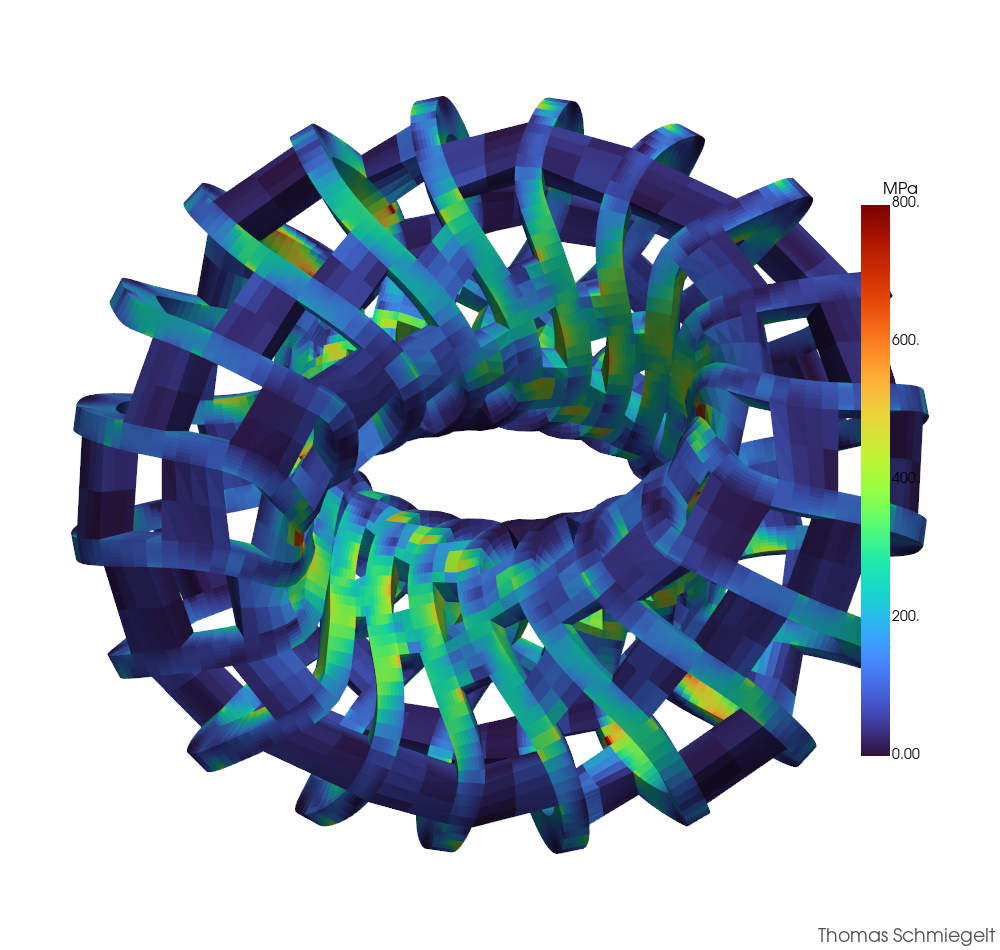
\includegraphics[width=\linewidth]{bilder/spannung_0157.png}\\\footnotesize von Mises stress in the steel (top view, 0–800 MPa)\end{minipage}\hfill
\begin{minipage}[t]{0.49\linewidth}\centering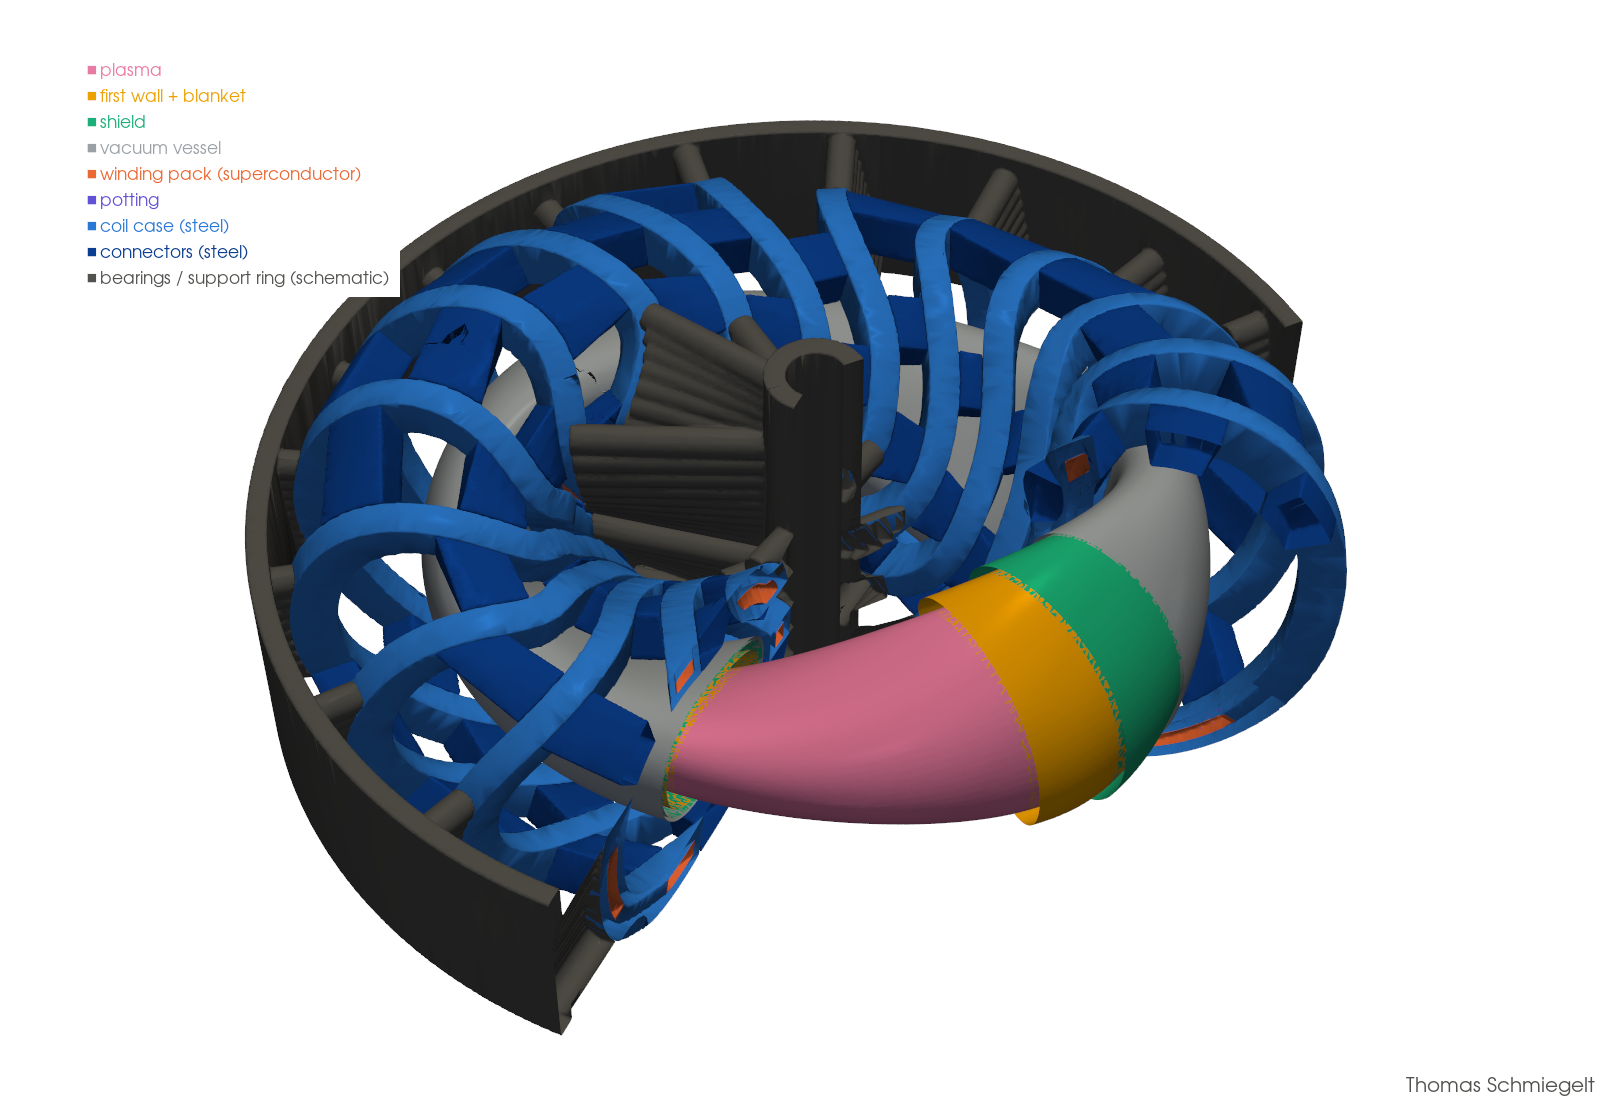
\includegraphics[width=\linewidth]{bilder/modell3d_0157_schnitt_en.png}\\\footnotesize PicoGK model, stepped cut\end{minipage}\hfill
\caption{Design 0157}\end{figure}
\clearpage
\subsection{Design 0063}\label{sb:0063}
\noindent\textbf{Verdict: }Admissible in doe1, no longer with the standard mesh: bottleneck winding-pack strain (reserve -24 \%).\par\smallskip
\begin{minipage}[t]{0.46\linewidth}\small\begin{tabular}[t]{@{}lr@{}}\toprule\multicolumn{2}{@{}l}{\textbf{Design variables}}\\\midrule
coil–plasma distance & \num{0.177} \\
coils in total & 20 \\
coils per half period & \num{5} \\
length per coil & \num{4.45} \\
force weight & \num{0.000} \\
inner wall & \num{0.59} \\
side wall & \num{0.35} \\
outer wall min. & \num{0.69} \\
outer wall extra & \num{0.44} \\
connector stiffness & \num{43} \\
connectors per pair & \num{14} \\
bearing radius & \num{1.71} \\
\bottomrule\end{tabular}\end{minipage}\hfill
\begin{minipage}[t]{0.5\linewidth}\small\begin{tabular}[t]{@{}lr@{}}\toprule\multicolumn{2}{@{}l}{\textbf{Results}}\\\midrule
$\sigma_{99}$ steel 1.4429 & \num{595} MPa \\
largest element & \num{4265} MPa \\
$P_m$ max. / 99 \% & \num{4261} / \num{942} MPa \\
$P_m+P_b$ max. & \num{4270} MPa \\
connectors σ99 & \num{200} MPa \\
max. deformation & \num{81} mm \\
winding-pack strain & \num{0.37} \% \\
current per coil & \num{17.7} MA \\
field at conductor & \num{17.5} T \\
utilisation / margin & \num{33} \% / \num{22} K \\
field error $B\cdot n$ & \num{0.75} ‰ \\
clearance plasma–case & \num{1.53} m \\
nuclear heating / fluence & \num{24} W/m³ / 2.0e17 \\
steel case + connectors & \num{16.7} + \num{24.2} kt \\
connectors built & 252 \\
\bottomrule\end{tabular}\end{minipage}\par\medskip
\noindent\textit{Mesh study ($\sigma_{99}$/max. in MPa): }doe1: 369/2016; standard: 595/4265.\par\smallskip
\begin{figure}[H]\centering
\begin{minipage}[t]{0.49\linewidth}\centering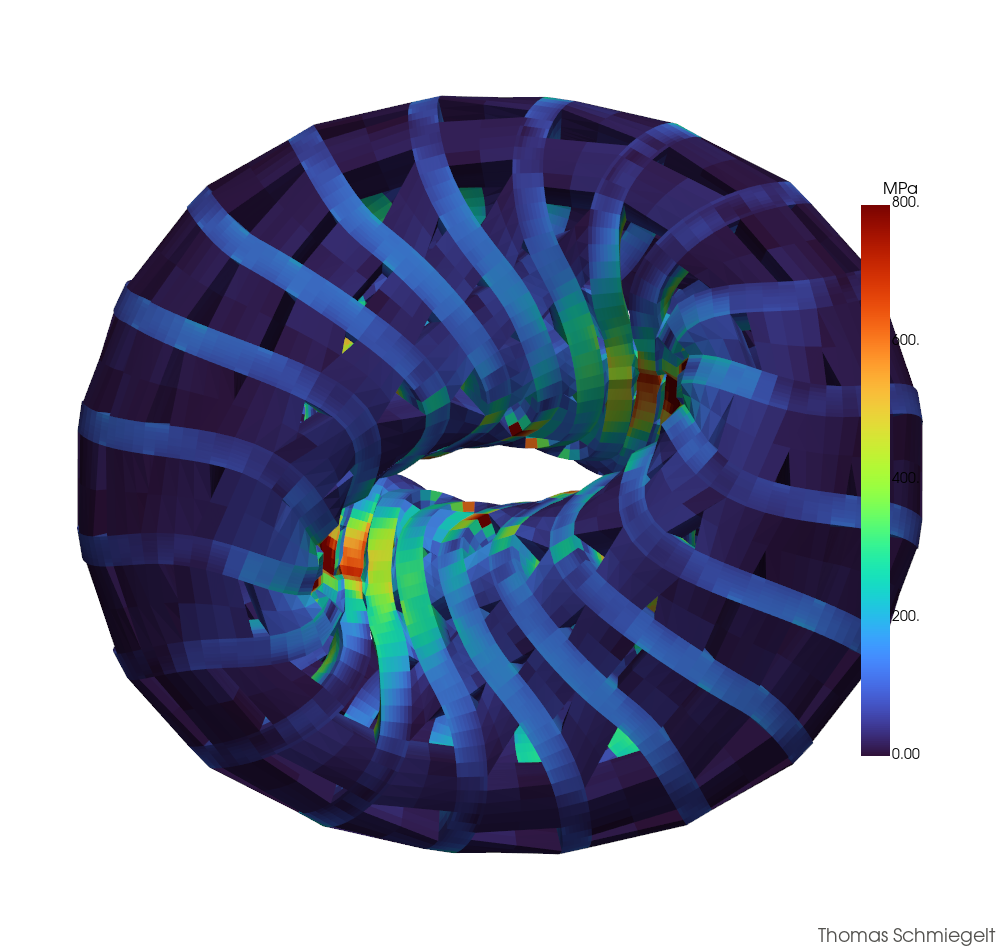
\includegraphics[width=\linewidth]{bilder/spannung_0063.png}\\\footnotesize von Mises stress in the steel (top view, 0–800 MPa)\end{minipage}\hfill
\begin{minipage}[t]{0.49\linewidth}\centering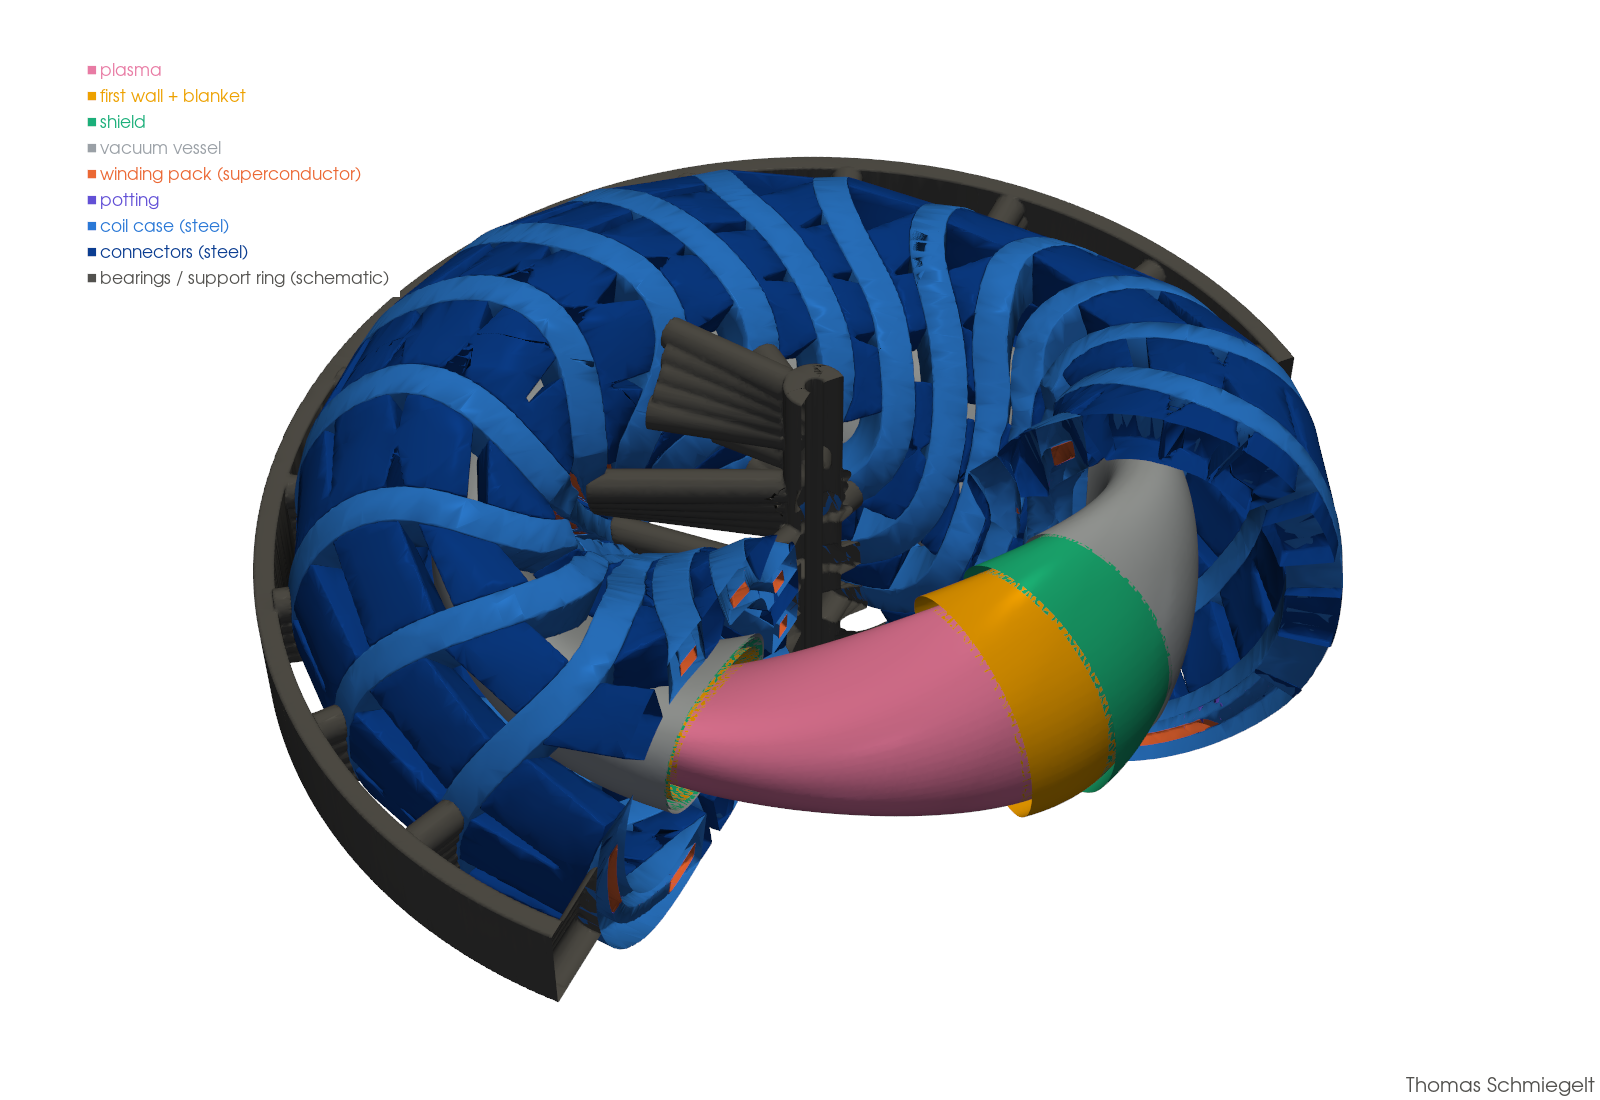
\includegraphics[width=\linewidth]{bilder/modell3d_0063_schnitt_en.png}\\\footnotesize PicoGK model, stepped cut\end{minipage}\hfill
\caption{Design 0063}\end{figure}
\clearpage
\subsection{Design 0136}\label{sb:0136}
\noindent\textbf{Verdict: }Admissible in doe1, no longer with the standard mesh: bottleneck σ99 steel 1.4429 (reserve -15 \%).\par\smallskip
\begin{minipage}[t]{0.46\linewidth}\small\begin{tabular}[t]{@{}lr@{}}\toprule\multicolumn{2}{@{}l}{\textbf{Design variables}}\\\midrule
coil–plasma distance & \num{0.232} \\
coils in total & 20 \\
coils per half period & \num{5} \\
length per coil & \num{4.51} \\
force weight & \num{0.012} \\
inner wall & \num{0.16} \\
side wall & \num{0.30} \\
outer wall min. & \num{0.57} \\
outer wall extra & \num{0.22} \\
connector stiffness & \num{21} \\
connectors per pair & \num{13} \\
bearing radius & \num{3.12} \\
\bottomrule\end{tabular}\end{minipage}\hfill
\begin{minipage}[t]{0.5\linewidth}\small\begin{tabular}[t]{@{}lr@{}}\toprule\multicolumn{2}{@{}l}{\textbf{Results}}\\\midrule
$\sigma_{99}$ steel 1.4429 & \num{577} MPa \\
largest element & \num{2238} MPa \\
$P_m$ max. / 99 \% & \num{2201} / \num{690} MPa \\
$P_m+P_b$ max. & \num{2291} MPa \\
connectors σ99 & \num{141} MPa \\
max. deformation & \num{54} mm \\
winding-pack strain & \num{0.30} \% \\
current per coil & \num{17.7} MA \\
field at conductor & \num{16.9} T \\
utilisation / margin & \num{32} \% / \num{23} K \\
field error $B\cdot n$ & \num{1.62} ‰ \\
clearance plasma–case & \num{1.84} m \\
nuclear heating / fluence & \num{1} W/m³ / 9.6e15 \\
steel case + connectors & \num{10.0} + \num{16.3} kt \\
connectors built & 254 \\
\bottomrule\end{tabular}\end{minipage}\par\medskip
\noindent\textit{Mesh study ($\sigma_{99}$/max. in MPa): }doe1: 479/995; standard: 577/2238.\par\smallskip
\begin{figure}[H]\centering
\begin{minipage}[t]{0.49\linewidth}\centering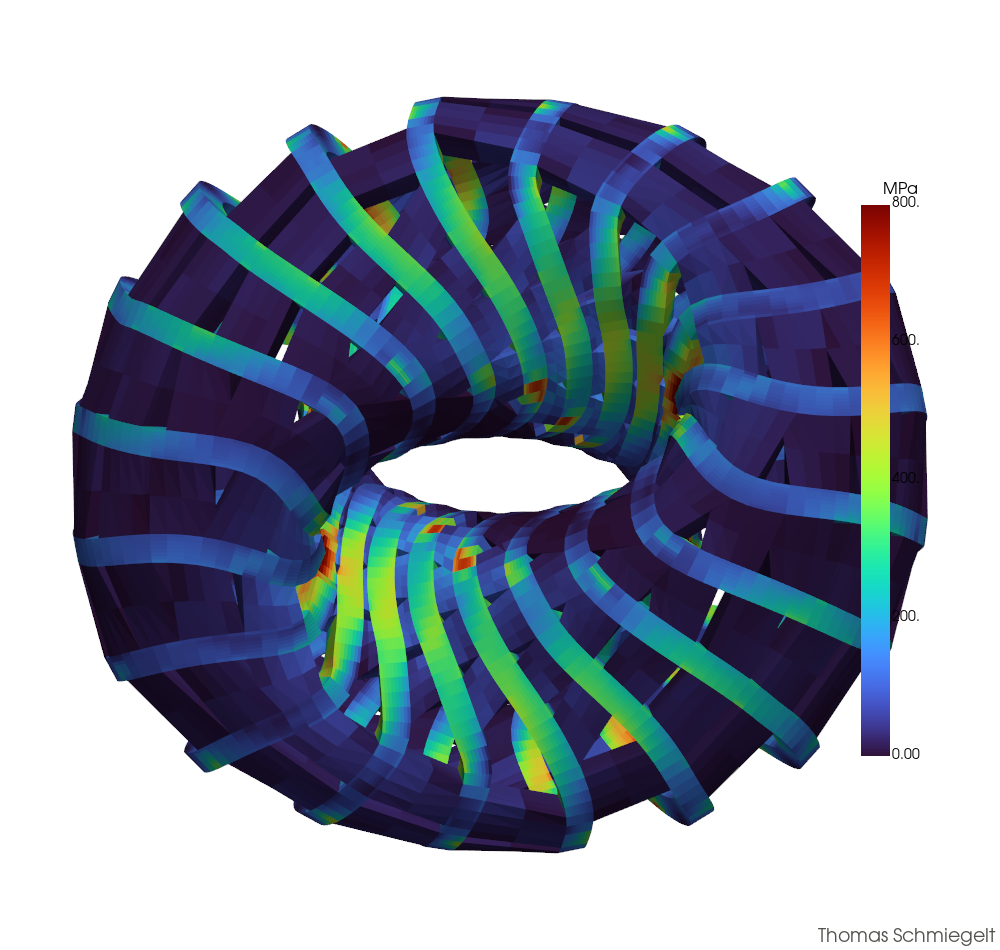
\includegraphics[width=\linewidth]{bilder/spannung_0136.png}\\\footnotesize von Mises stress in the steel (top view, 0–800 MPa)\end{minipage}\hfill
\begin{minipage}[t]{0.49\linewidth}\centering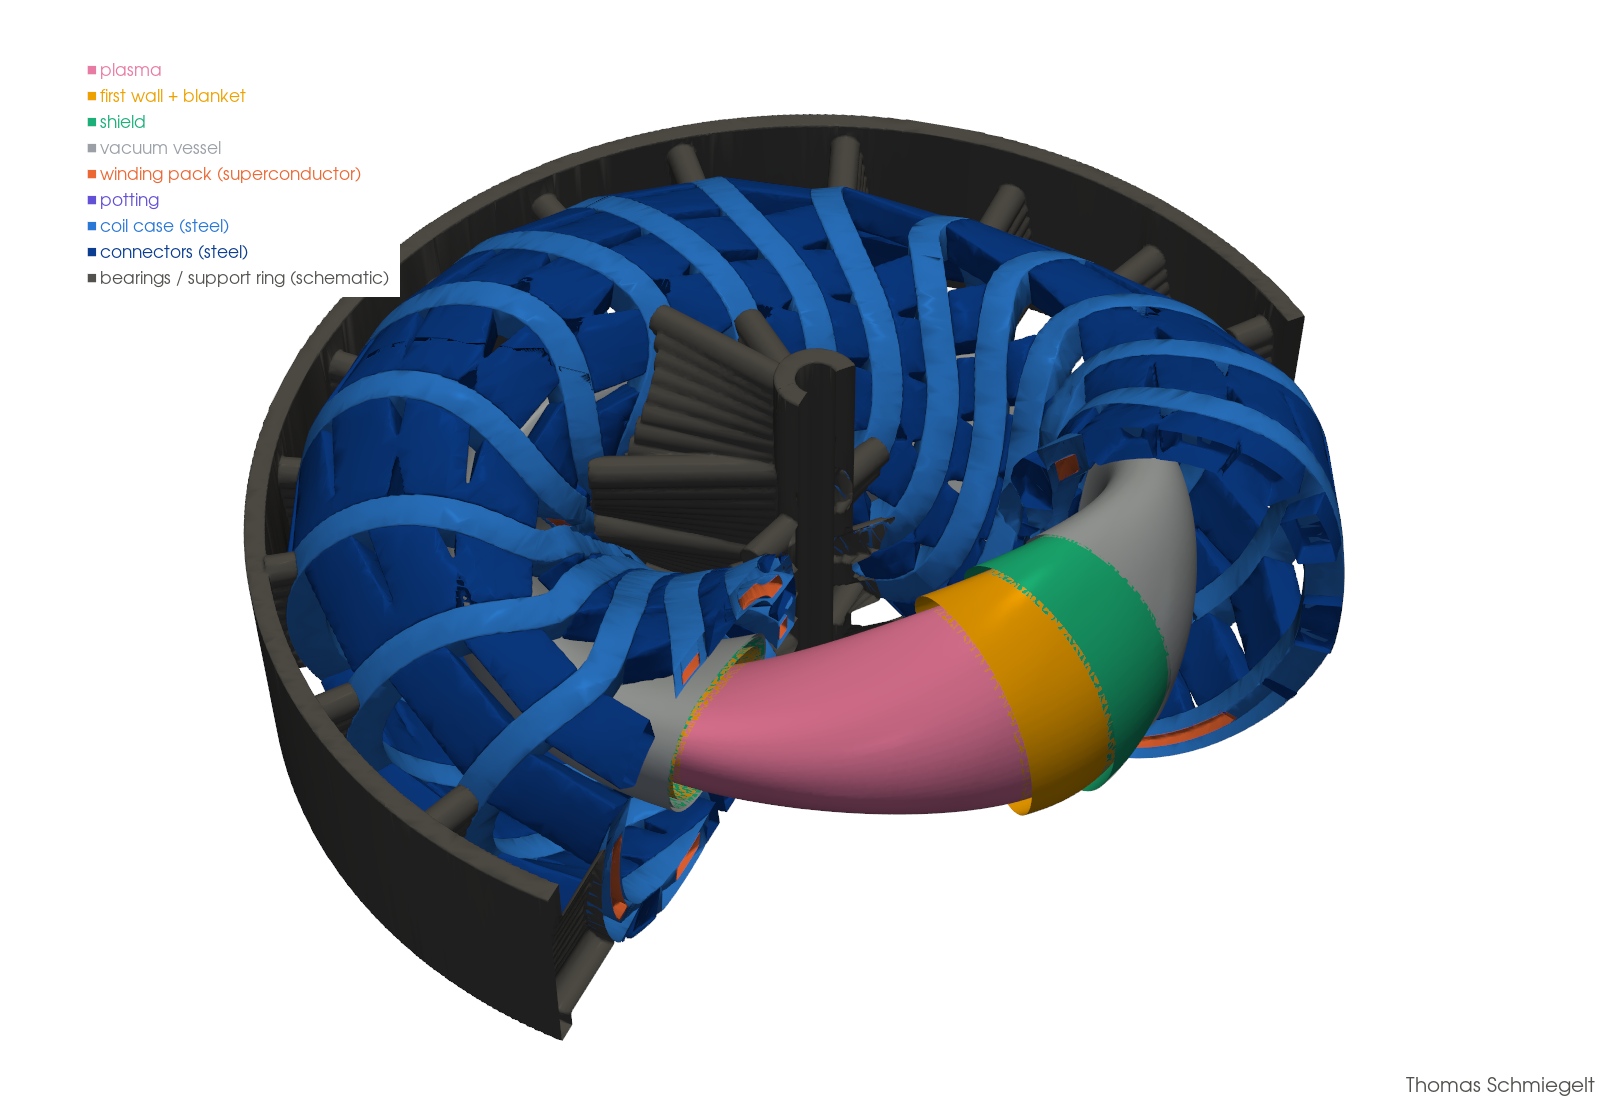
\includegraphics[width=\linewidth]{bilder/modell3d_0136_schnitt_en.png}\\\footnotesize PicoGK model, stepped cut\end{minipage}\hfill
\caption{Design 0136}\end{figure}
\clearpage
\subsection{Surrogate proposal V3}\label{sb:V3}
\noindent\textbf{Verdict: }Surrogate proposal (section~\ref{sec:ersatz1}), admissible; smallest reserve 35 \% (field error B·n).\par\smallskip
\begin{minipage}[t]{0.46\linewidth}\small\begin{tabular}[t]{@{}lr@{}}\toprule\multicolumn{2}{@{}l}{\textbf{Design variables}}\\\midrule
coil–plasma distance & \num{0.205} \\
coils in total & 24 \\
coils per half period & \num{6} \\
length per coil & \num{4.15} \\
force weight & \num{0.022} \\
inner wall & \num{0.20} \\
side wall & \num{0.24} \\
outer wall min. & \num{0.77} \\
outer wall extra & \num{0.48} \\
connector stiffness & \num{176} \\
connectors per pair & \num{11} \\
bearing radius & \num{3.02} \\
\bottomrule\end{tabular}\end{minipage}\hfill
\begin{minipage}[t]{0.5\linewidth}\small\begin{tabular}[t]{@{}lr@{}}\toprule\multicolumn{2}{@{}l}{\textbf{Results}}\\\midrule
$\sigma_{99}$ steel 1.4429 & \num{272} MPa \\
largest element & \num{656} MPa \\
$P_m$ max. / 99 \% & \num{621} / \num{302} MPa \\
$P_m+P_b$ max. & \num{724} MPa \\
connectors σ99 & \num{178} MPa \\
max. deformation & \num{13} mm \\
winding-pack strain & \num{0.13} \% \\
current per coil & \num{14.7} MA \\
field at conductor & \num{15.6} T \\
utilisation / margin & \num{30} \% / \num{24} K \\
field error $B\cdot n$ & \num{1.96} ‰ \\
clearance plasma–case & \num{1.54} m \\
nuclear heating / fluence & \num{22} W/m³ / 1.8e17 \\
steel case + connectors & \num{12.3} + \num{16.8} kt \\
connectors built & 256 \\
\bottomrule\end{tabular}\end{minipage}\par\medskip
\noindent\textit{Mesh study ($\sigma_{99}$/max. in MPa): }standard: 272/656; 1.5× stations: 394/1841.\par\smallskip
\begin{figure}[H]\centering
\begin{minipage}[t]{0.49\linewidth}\centering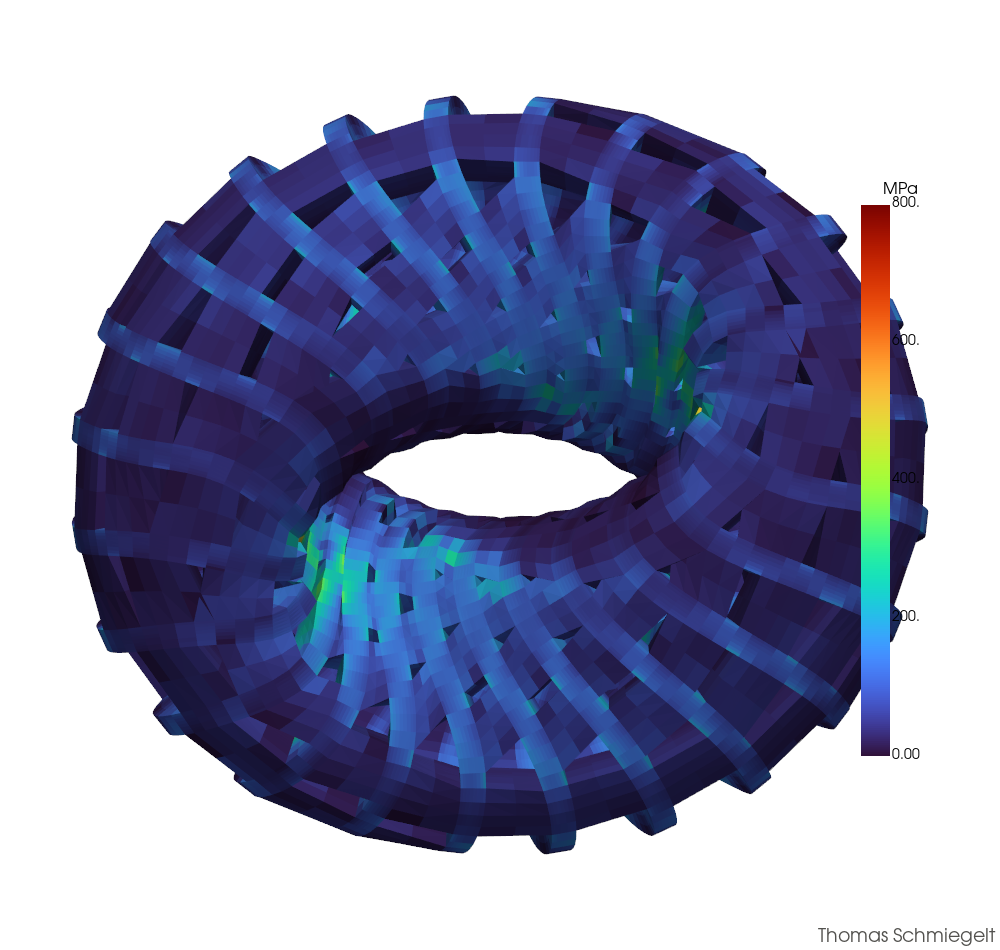
\includegraphics[width=\linewidth]{bilder/spannung_V3.png}\\\footnotesize von Mises stress in the steel (top view, 0–800 MPa)\end{minipage}\hfill
\begin{minipage}[t]{0.49\linewidth}\centering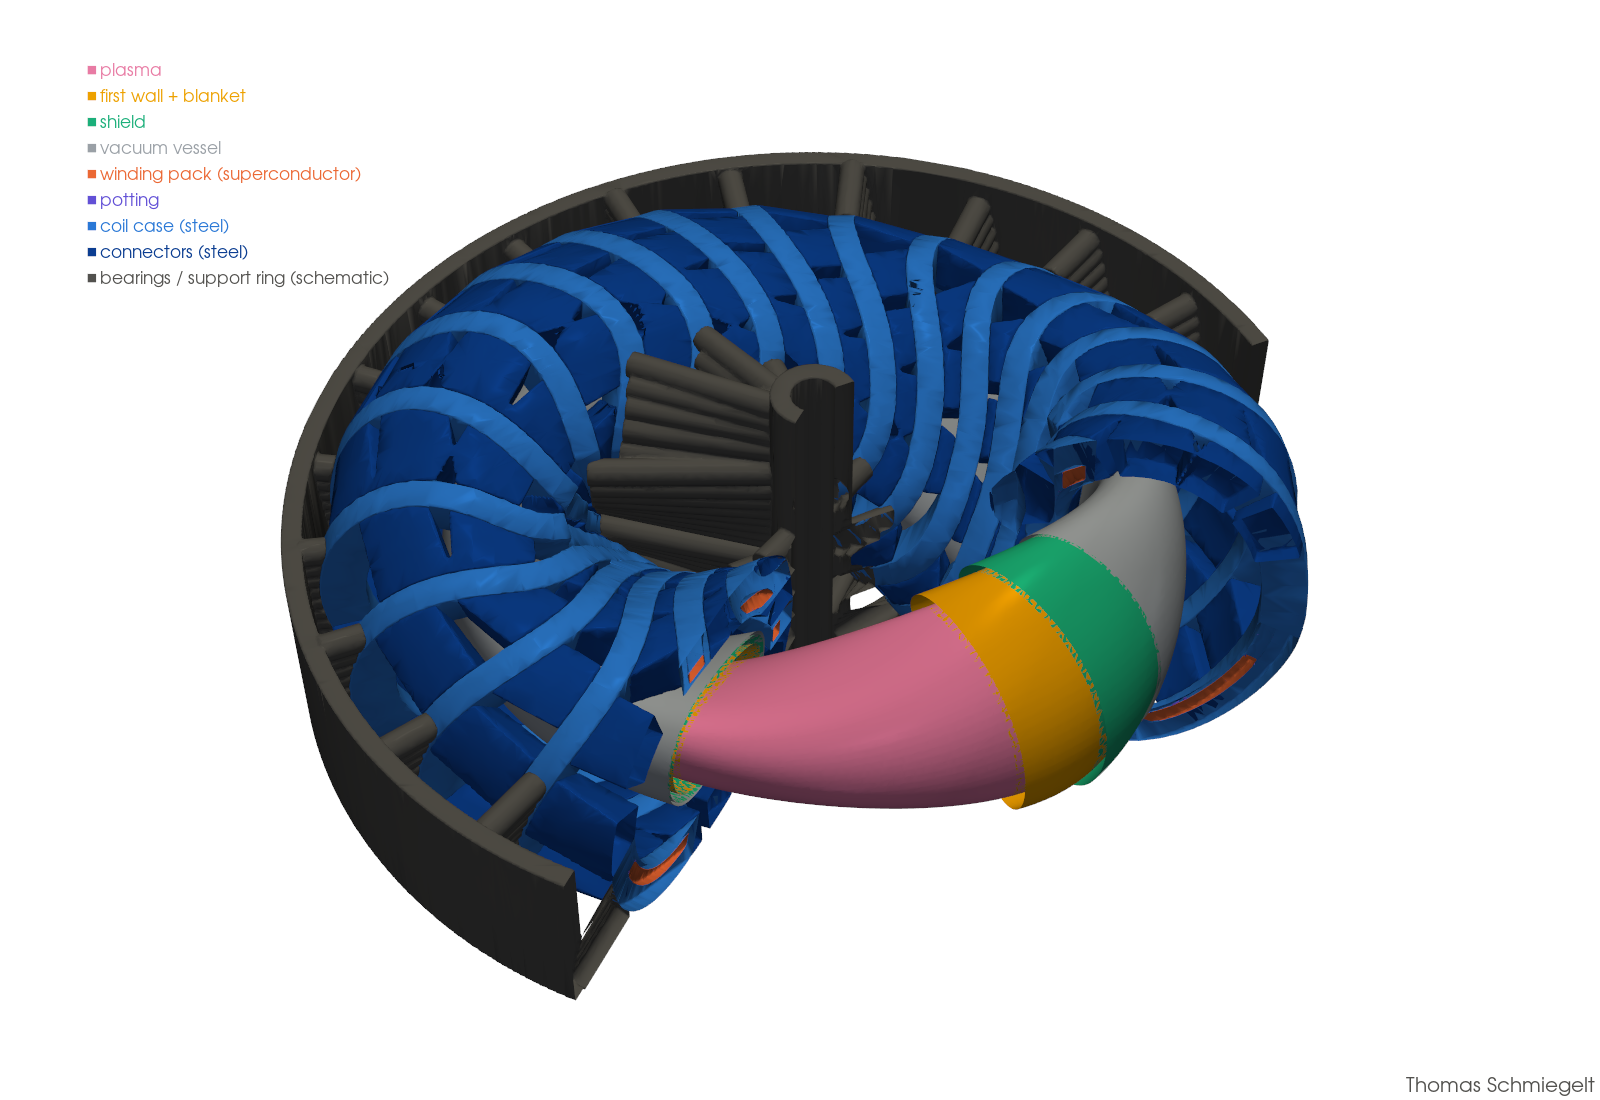
\includegraphics[width=\linewidth]{bilder/modell3d_V3_schnitt_en.png}\\\footnotesize PicoGK model, stepped cut\end{minipage}\hfill
\caption{Surrogate proposal V3}\end{figure}
\clearpage
\subsection{Surrogate proposal V1}\label{sb:V1}
\noindent\textbf{Verdict: }Surrogate proposal (section~\ref{sec:ersatz1}), admissible; smallest reserve 31 \% (package space).\par\smallskip
\begin{minipage}[t]{0.46\linewidth}\small\begin{tabular}[t]{@{}lr@{}}\toprule\multicolumn{2}{@{}l}{\textbf{Design variables}}\\\midrule
coil–plasma distance & \num{0.208} \\
coils in total & 24 \\
coils per half period & \num{6} \\
length per coil & \num{3.98} \\
force weight & \num{0.023} \\
inner wall & \num{0.36} \\
side wall & \num{0.32} \\
outer wall min. & \num{0.77} \\
outer wall extra & \num{0.33} \\
connector stiffness & \num{77} \\
connectors per pair & \num{13} \\
bearing radius & \num{3.41} \\
\bottomrule\end{tabular}\end{minipage}\hfill
\begin{minipage}[t]{0.5\linewidth}\small\begin{tabular}[t]{@{}lr@{}}\toprule\multicolumn{2}{@{}l}{\textbf{Results}}\\\midrule
$\sigma_{99}$ steel 1.4429 & \num{220} MPa \\
largest element & \num{637} MPa \\
$P_m$ max. / 99 \% & \num{532} / \num{248} MPa \\
$P_m+P_b$ max. & \num{746} MPa \\
connectors σ99 & \num{111} MPa \\
max. deformation & \num{11} mm \\
winding-pack strain & \num{0.12} \% \\
current per coil & \num{14.7} MA \\
field at conductor & \num{15.6} T \\
utilisation / margin & \num{30} \% / \num{24} K \\
field error $B\cdot n$ & \num{1.87} ‰ \\
clearance plasma–case & \num{1.41} m \\
nuclear heating / fluence & \num{85} W/m³ / 7.1e17 \\
steel case + connectors & \num{14.6} + \num{18.5} kt \\
connectors built & 308 \\
\bottomrule\end{tabular}\end{minipage}\par\medskip
\noindent\textit{Mesh study ($\sigma_{99}$/max. in MPa): }standard: 220/637; 1.5× stations: 366/2185.\par\smallskip
\begin{figure}[H]\centering
\begin{minipage}[t]{0.49\linewidth}\centering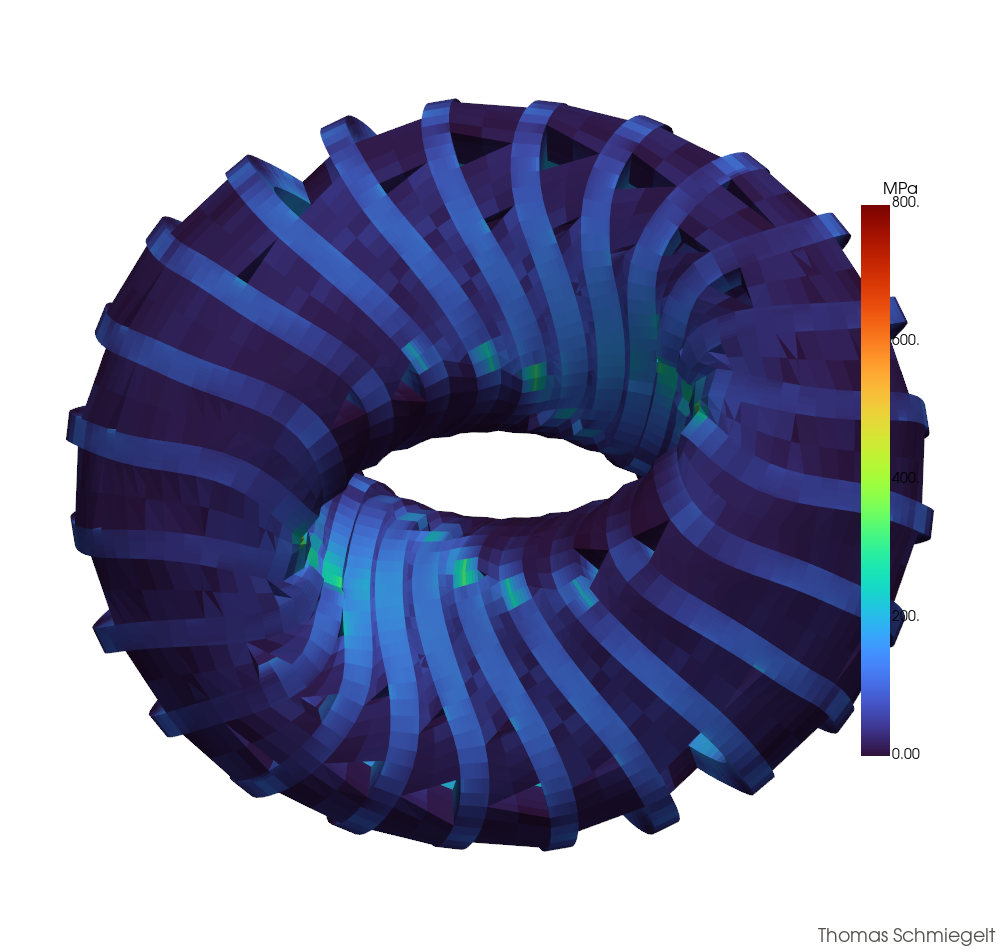
\includegraphics[width=\linewidth]{bilder/spannung_V1.png}\\\footnotesize von Mises stress in the steel (top view, 0–800 MPa)\end{minipage}\hfill
\begin{minipage}[t]{0.49\linewidth}\centering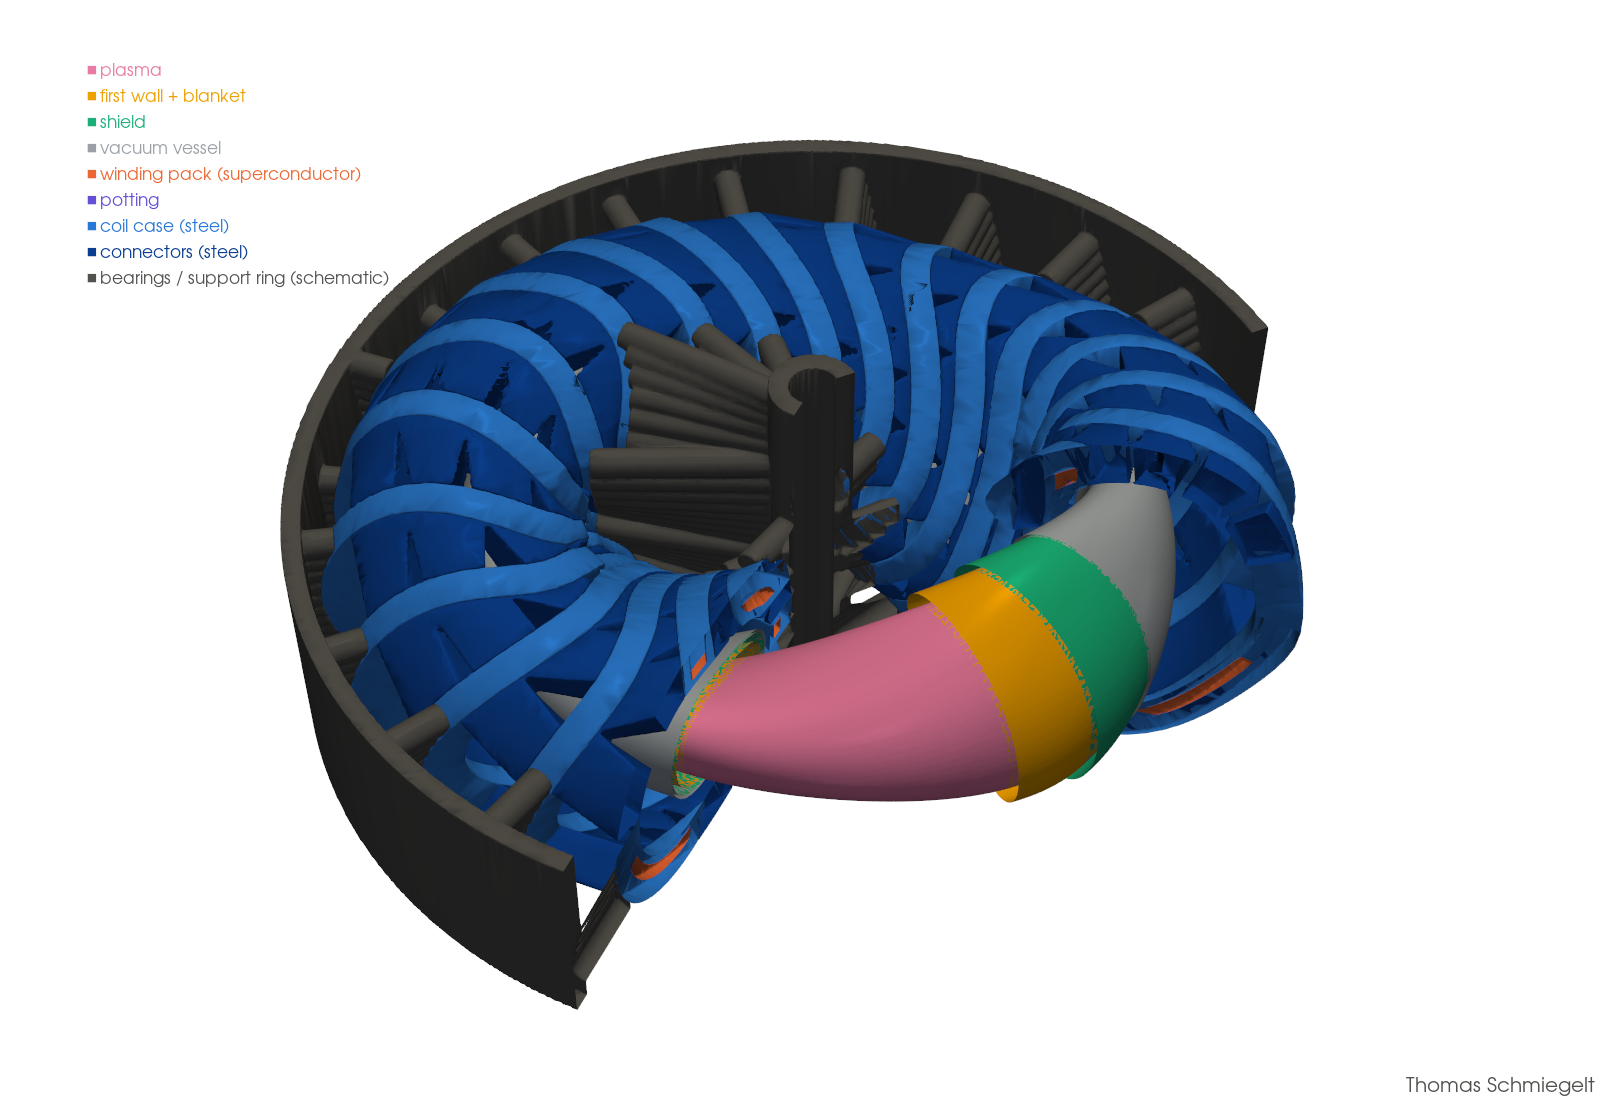
\includegraphics[width=\linewidth]{bilder/modell3d_V1_schnitt_en.png}\\\footnotesize PicoGK model, stepped cut\end{minipage}\hfill
\caption{Surrogate proposal V1}\end{figure}
\clearpage
\subsection{Support test E (thickest walls)}\label{sb:E_test}
\noindent\textbf{Verdict: }Same 16 coils as the starting design; only the support structure differs.\par\smallskip
\begin{minipage}[t]{0.46\linewidth}\small\begin{tabular}[t]{@{}lr@{}}\toprule\multicolumn{2}{@{}l}{\textbf{Design variables}}\\\midrule
coil–plasma distance & \num{0.180} \\
coils in total & 16 \\
coils per half period & \num{4} \\
length per coil & \num{4.50} \\
force weight & \num{0.000} \\
inner wall & \num{0.60} \\
side wall & \num{0.40} \\
outer wall min. & \num{0.80} \\
outer wall extra & \num{0.60} \\
connector stiffness & \num{200} \\
connectors per pair & \num{12} \\
bearing radius & \num{2.50} \\
\bottomrule\end{tabular}\end{minipage}\hfill
\begin{minipage}[t]{0.5\linewidth}\small\begin{tabular}[t]{@{}lr@{}}\toprule\multicolumn{2}{@{}l}{\textbf{Results}}\\\midrule
$\sigma_{99}$ steel 1.4429 & \num{481} MPa \\
largest element & \num{2455} MPa \\
$P_m$ max. / 99 \% & \num{2396} / \num{736} MPa \\
$P_m+P_b$ max. & \num{2515} MPa \\
connectors σ99 & \num{276} MPa \\
max. deformation & \num{41} mm \\
winding-pack strain & \num{0.31} \% \\
current per coil & \num{22.1} MA \\
field at conductor & \num{18.7} T \\
utilisation / margin & \num{34} \% / \num{22} K \\
field error $B\cdot n$ & \num{2.71} ‰ \\
clearance plasma–case & \num{1.53} m \\
nuclear heating / fluence & \num{25} W/m³ / 2.1e17 \\
steel case + connectors & \num{17.6} + \num{19.4} kt \\
connectors built & 168 \\
\bottomrule\end{tabular}\end{minipage}\par\medskip
\begin{figure}[H]\centering
\begin{minipage}[t]{0.49\linewidth}\centering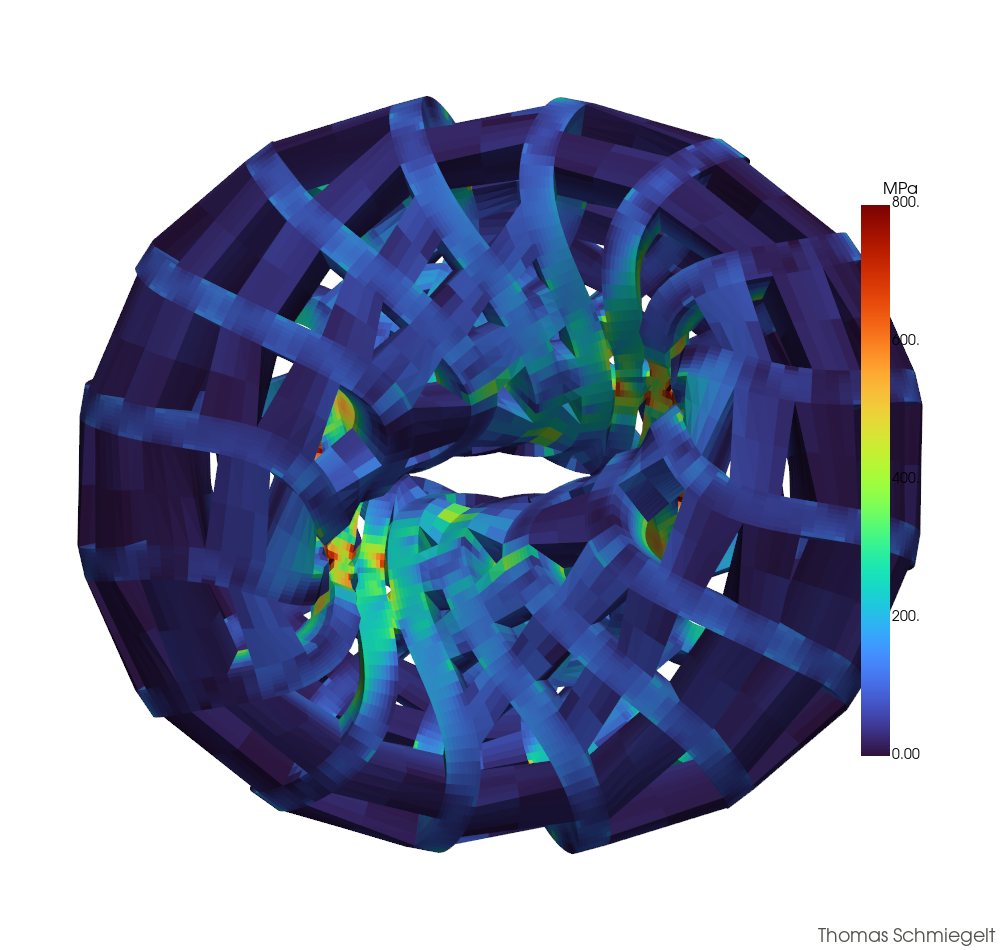
\includegraphics[width=\linewidth]{bilder/spannung_E_test.png}\\\footnotesize von Mises stress in the steel (top view, 0–800 MPa)\end{minipage}\hfill
\begin{minipage}[t]{0.49\linewidth}\centering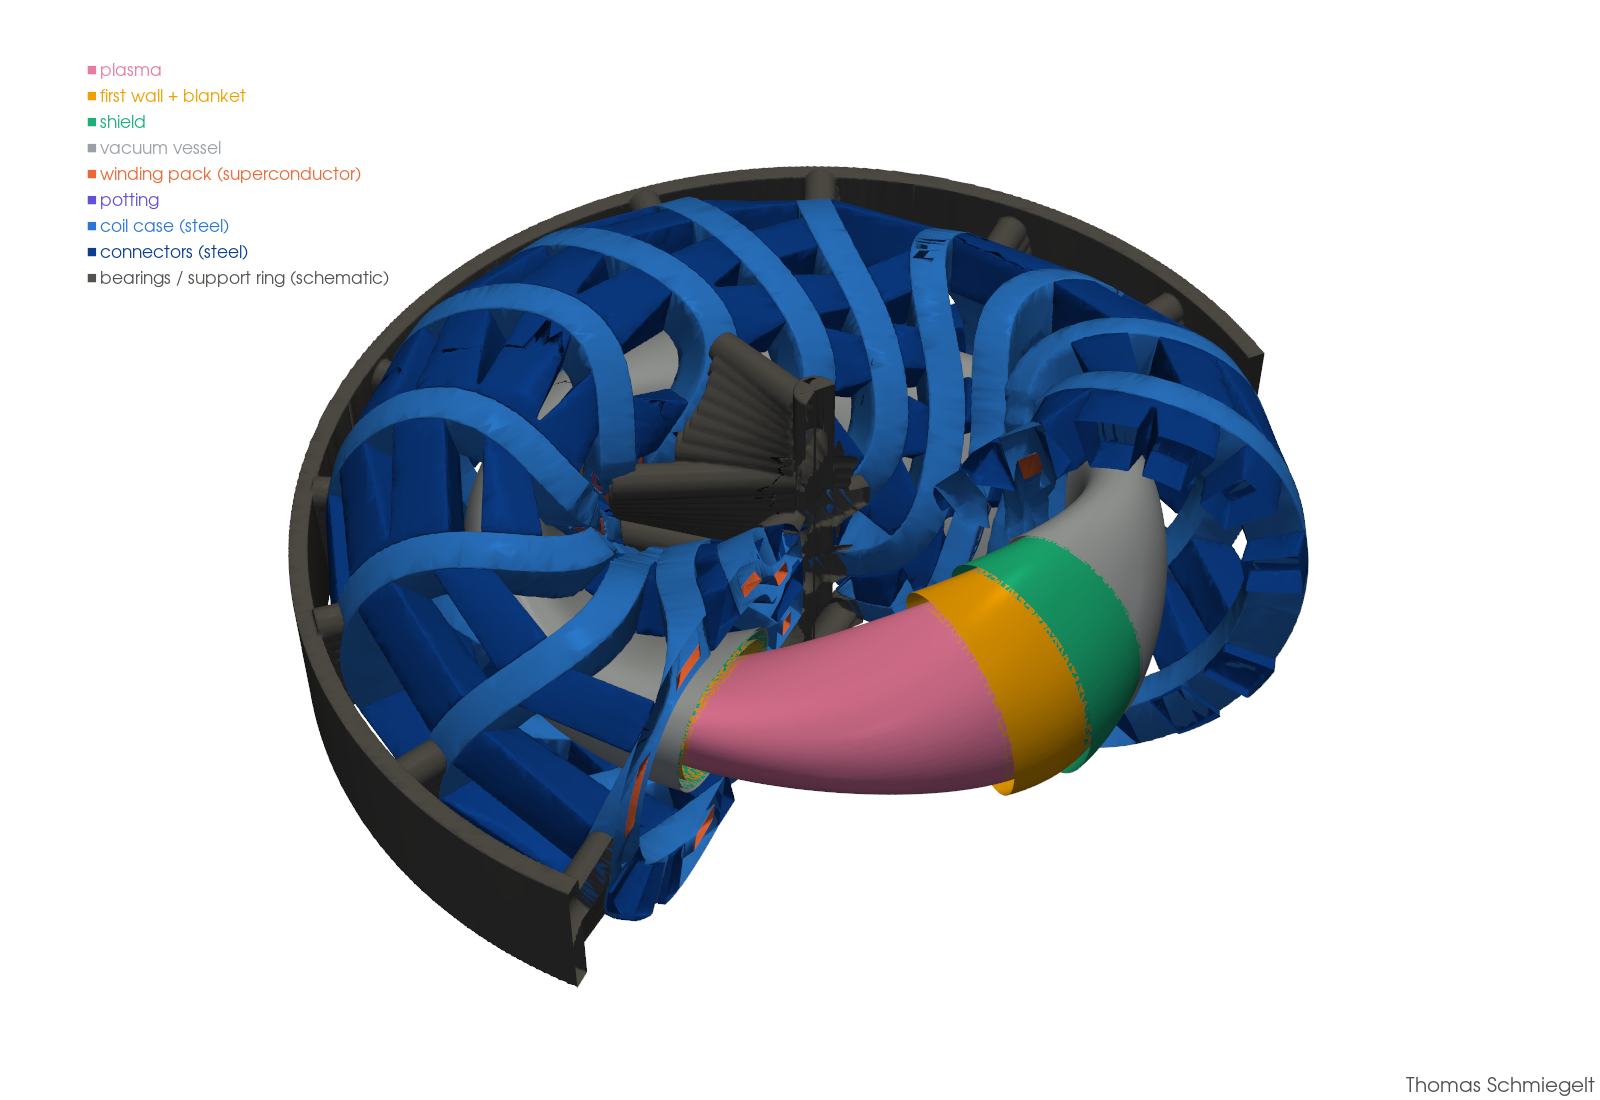
\includegraphics[width=\linewidth]{bilder/modell3d_E_test_schnitt_en.png}\\\footnotesize PicoGK model, stepped cut\end{minipage}\hfill
\caption{Support test E (thickest walls)}\end{figure}
\clearpage
\subsection{Support test A (starting design)}\label{sb:A_test}
\noindent\textbf{Verdict: }Same 16 coils as the starting design; only the support structure differs.\par\smallskip
\begin{minipage}[t]{0.46\linewidth}\small\begin{tabular}[t]{@{}lr@{}}\toprule\multicolumn{2}{@{}l}{\textbf{Design variables}}\\\midrule
coil–plasma distance & \num{0.180} \\
coils in total & 16 \\
coils per half period & \num{4} \\
length per coil & \num{4.50} \\
force weight & \num{0.000} \\
inner wall & \num{0.35} \\
side wall & \num{0.24} \\
outer wall min. & \num{0.45} \\
outer wall extra & \num{0.30} \\
connector stiffness & \num{50} \\
connectors per pair & \num{6} \\
bearing radius & \num{2.50} \\
\bottomrule\end{tabular}\end{minipage}\hfill
\begin{minipage}[t]{0.5\linewidth}\small\begin{tabular}[t]{@{}lr@{}}\toprule\multicolumn{2}{@{}l}{\textbf{Results}}\\\midrule
$\sigma_{99}$ steel 1.4429 & \num{2129} MPa \\
largest element & \num{8454} MPa \\
connectors σ99 & \num{675} MPa \\
max. deformation & \num{399} mm \\
winding-pack strain & \num{0.76} \% \\
current per coil & \num{22.1} MA \\
field at conductor & \num{18.7} T \\
utilisation / margin & \num{34} \% / \num{22} K \\
field error $B\cdot n$ & \num{2.71} ‰ \\
clearance plasma–case & \num{1.77} m \\
nuclear heating / fluence & \num{2} W/m³ / 1.8e16 \\
steel case + connectors & \num{8.5} + \num{7.0} kt \\
connectors built & 90 \\
\bottomrule\end{tabular}\end{minipage}\par\medskip
\begin{figure}[H]\centering
\begin{minipage}[t]{0.49\linewidth}\centering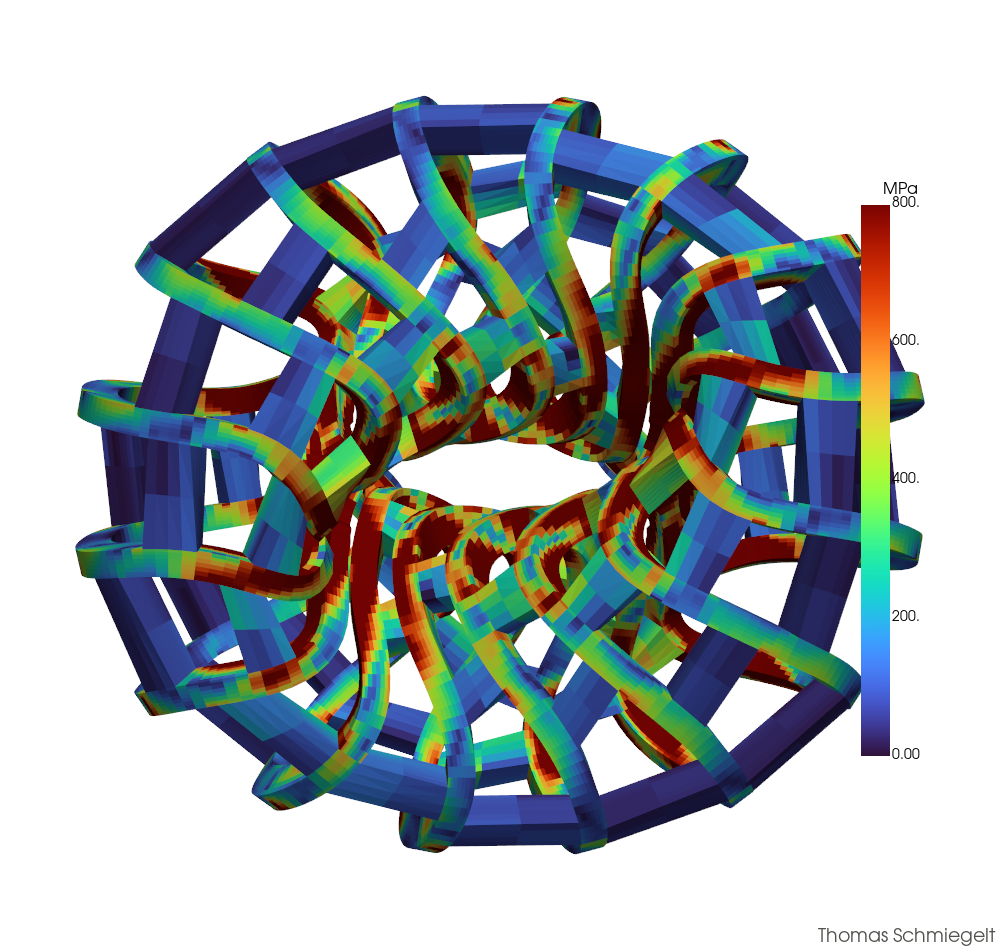
\includegraphics[width=\linewidth]{bilder/spannung_A_test.png}\\\footnotesize von Mises stress in the steel (top view, 0–800 MPa)\end{minipage}\hfill
\begin{minipage}[t]{0.49\linewidth}\centering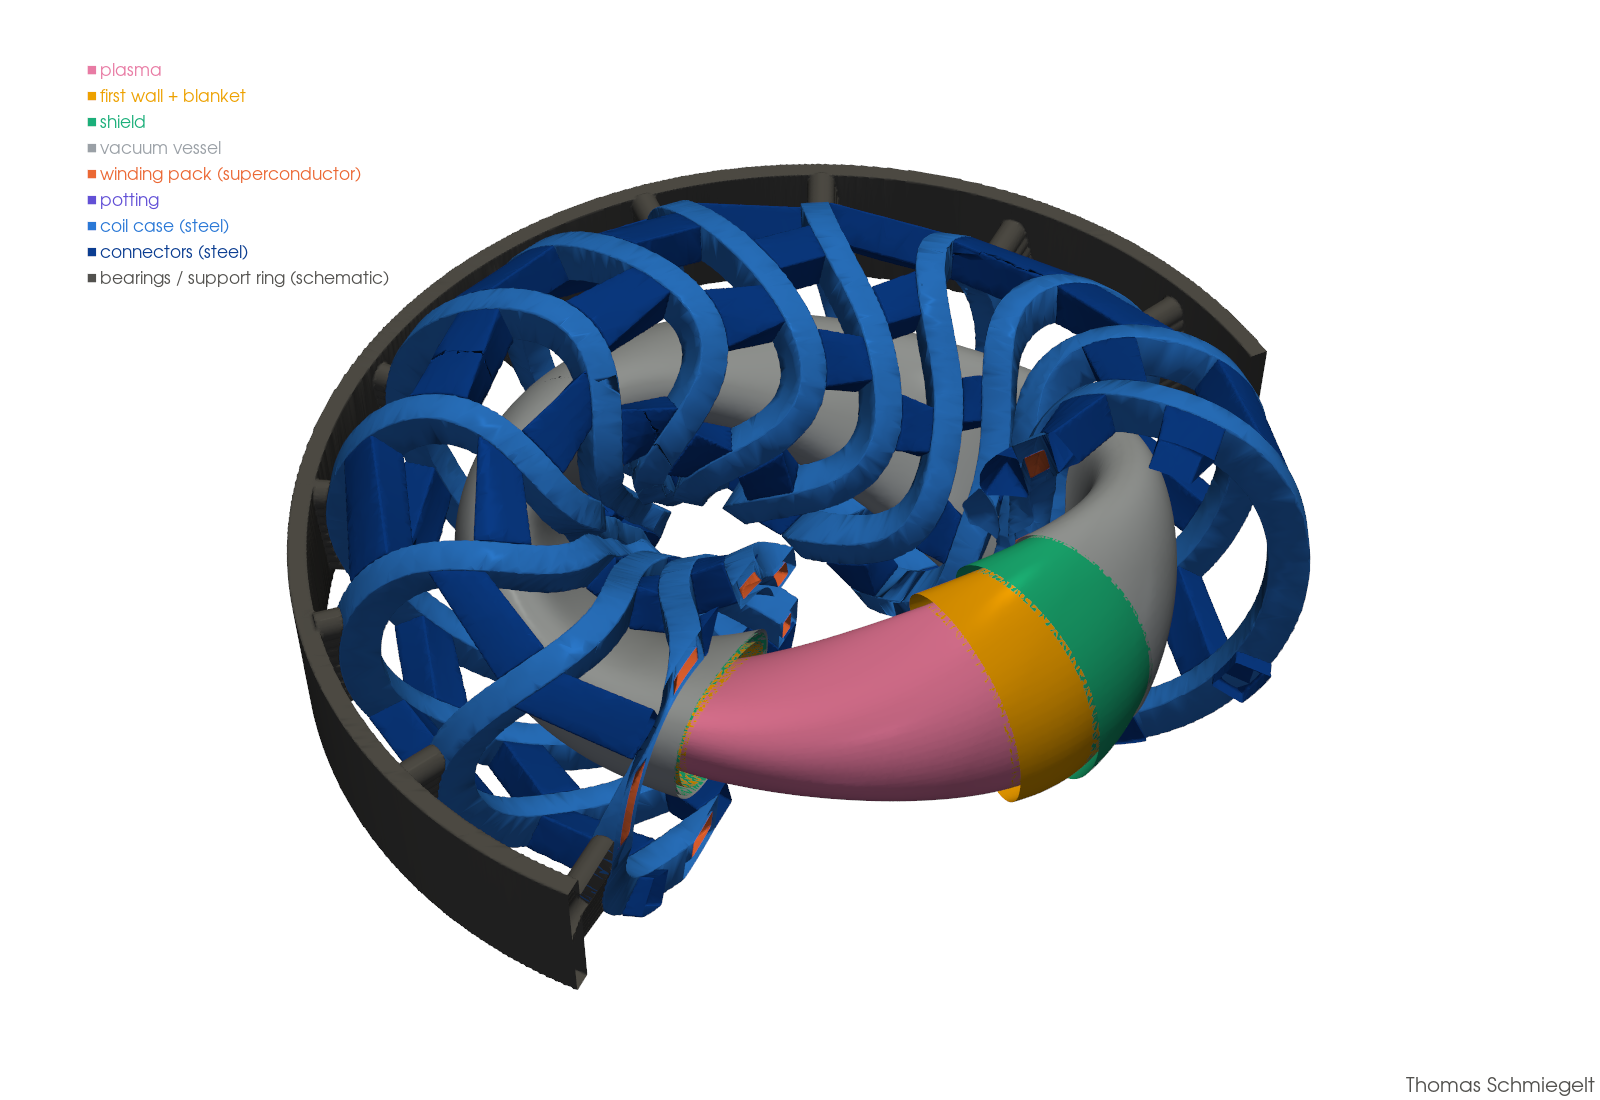
\includegraphics[width=\linewidth]{bilder/modell3d_A_test_schnitt_en.png}\\\footnotesize PicoGK model, stepped cut\end{minipage}\hfill
\caption{Support test A (starting design)}\end{figure}


%======================================================================
\section{Comparison and conclusions}\label{sec:vergleich}
\paragraph{Which design is the most robust?} At the user's request the goal was not the lightest design but the one
with the largest reserve against all eight limits (``weight is not that important, it is a building''). After the
clean-up seven designs meet all limits. Their smallest reserve (robustness) ranges from 0.30 (0061) to 0.02 (0157).
Two designs are almost level: 0061 (bottleneck steel) and 0169 (bottleneck package thickness). The mesh study
decides (section~\ref{sec:netz}):

\begin{itemize}
\item \textbf{0169} stays practically unchanged on a finer mesh (\SI{308}{} $\to$ \SI{319}{MPa}, $+4$~\%). Its
  reserve does not depend on numerical accuracy; its bottleneck is the package thickness, which depends on
  geometry, not on the mesh. It is therefore the \textbf{recommended design}: 24 coils, 13 stiff connectors per
  coil pair, about \SI{28}{kt} of steel.
\item \textbf{0061} has the largest reserve on the standard mesh but rises by $+58$~\% on the fine mesh
  (\SI{351}{} $\to$ \SI{556}{MPa}) and then exceeds the limit. Its bottleneck is exactly the mesh-dependent
  quantity.
\item \textbf{0093, 0008, 0014} rise by 34--46~\% on the fine mesh and end up partly just below, partly above the
  limit. They are candidates, but only after a more accurate analysis of the connector joints.
\item \textbf{0017, 0157} have little reserve and were not refined further.
\item \textbf{V3, V1} (surrogate proposals) are more robust than 0169 on the standard mesh (0.35 and 0.31), but on
  the fine mesh their stress rises by 45 and 66~\% (section~\ref{sec:ersatz1}). V3 thus drops to 0.21.
\end{itemize}

\paragraph{Narrow misses.} The five most robust inadmissible designs (0173, 0103, 0044, 0004, 0136) fail almost
all on steel stress or on the field error $B_n$. 0063 and 0136 were admissible on the coarse mesh and dropped out
after recomputation -- an example of how easily an unnoticed change of mesh flatters the result.

\paragraph{What distinguishes the variants.} Across all 198 designs:
\begin{enumerate}
\item \textbf{Number of coils:} no design with 16 coils was admissible. The coils become so long and so strongly
  curved that the cases bend too much, and the field error is larger. 20 and 24 coils split the force over more
  and shorter members.
\item \textbf{Coil shape before structure:} coil--plasma distance and coil length determine the stress more than
  number or stiffness of the connectors. The structure can compensate an unfavourable coil shape only to a limited
  extent.
\item \textbf{Package and nuclear heating} are almost purely geometric and are predicted very well by the surrogate
  ($R^2 \approx 0.98$). They can be screened reliably before any strength analysis.
\item \textbf{Stress} is predicted only roughly by the surrogate ($R^2 \approx 0.46$) because it depends on local
  peaks at the connector joints. Here the FE analysis remains indispensable.
\item \textbf{Softer connectors} (user idea ``weaken selectively'', first form) increase the stress. The idea has to
  be applied locally: soft ends, stiff core.
\end{enumerate}

\paragraph{How reliable is this?} The numbers come from a simplified model: cases as rectangular cross-sections,
connectors as beam bundles, supports as fixed points, only the magnetic force in cold operation (no cool-down
stress, no dead weight, no fatigue). The finer mesh shows that the peaks are not yet converged. The statement
``0169 is robust, 16 coils do not work'' is reliable because it holds on all meshes; the exact megapascals are not
yet.

\paragraph{Next steps.}
\begin{enumerate}
\item Compute 0169 with locally graded connectors (soft ends) and rounded joints; adapt stiffnesses iteratively by
  the stress ratio.
\item Test the conjecture that 0169 is mesh-stable because its connectors merge into almost continuous plates:
  compute 0169 once with non-overlapping connectors and once with a deliberately continuous plate.
\item Check mesh convergence at the connector joints of 0169 and 0093 with targeted local refinement.
\item Add cool-down stress (\SI{293}{K} $\to$ \SI{4}{K}) and dead weight.
\item Reuse the PicoGK model of 0169 as the starting shape for supports, cooling channels and potting.
\end{enumerate}


%======================================================================
\appendix
\section{All designs of the study doe1}\label{anh:alle}
Abbreviations: dist.\ minimum coil--plasma distance (unit geometry), length per coil (unit geometry), force = force
weight, w.i./w.s.\ inner/side wall, t outer wall min., n\textsubscript{c} connectors per pair, E\textsubscript{c}
connector stiffness, R\textsubscript{b} bearing radius, clear.\ = clearance plasma--case, heat = nuclear heating of the
winding pack. Last column: \checkmark\ admissible, otherwise bottleneck. $^\ast$ = recomputed with the standard mesh.
{\scriptsize\setlength{\tabcolsep}{2.2pt}\begin{longtable}{@{}lrrrrrrrrrrrrrrrrrl@{}}\toprule
No. & coils & dist. & length & force & w.i. & w.s. & t & n\textsubscript{c} & E\textsubscript{c} & R\textsubscript{b} & $\sigma_{99}$ & max. & strain & $B\cdot n$ & clear. & heat & steel & ok \\
 & & – & – & – & m & m & m & & GPa & m & MPa & MPa & \% & ‰ & m & W/m³ & kt & \\\midrule\endhead
0000 & 24 & \num{0.18} & \num{4.4} & \num{0.024} & \num{0.10} & \num{0.35} & \num{0.58} & 10 & \num{70} & \num{2.5} & \num{840} & \num{3425} & \num{0.42} & \num{1.98} & \num{1.44} & \num{60} & \num{23} & stahl \\
0001 & 20 & \num{0.24} & \num{4.4} & \num{0.012} & \num{0.13} & \num{0.15} & \num{0.35} & 7 & \num{135} & \num{2.9} & \num{1456} & \num{3851} & \num{0.60} & \num{1.53} & \num{2.00} & \num{0} & \num{12} & stahl \\
0002 & 24 & \num{0.30} & \num{4.5} & \num{0.028} & \num{0.26} & \num{0.10} & \num{0.20} & 8 & \num{25} & \num{2.7} & \num{4721} & \num{13357} & \num{2.01} & \num{3.67} & \num{2.39} & \num{0} & \num{13} & stahl \\
0003 & 16 & \num{0.20} & \num{3.7} & \num{0.025} & \num{0.34} & \num{0.10} & \num{0.49} & 12 & \num{142} & \num{1.9} & \num{617} & \num{1361} & \num{0.26} & \num{9.48} & \num{1.40} & \num{90} & \num{20} & Bn \\
0004 & 20 & \num{0.19} & \num{4.6} & \num{0.012} & \num{0.12} & \num{0.08} & \num{0.50} & 10 & \num{148} & \num{3.2} & \num{558} & \num{1085} & \num{0.26} & \num{1.81} & \num{1.54} & \num{22} & \num{19} & stahl \\
0005 & 16 & \num{0.15} & \num{4.9} & \num{0.020} & \num{0.59} & \num{0.08} & \num{0.15} & 13 & \num{114} & \num{2.9} & \num{844} & \num{1847} & \num{0.35} & \num{2.40} & \num{1.26} & \num{372} & \num{23} & stahl \\
0006 & 24 & \num{0.12} & \num{4.4} & \num{0.012} & \num{0.50} & \num{0.14} & \num{0.18} & 6 & \num{78} & \num{2.9} & \num{536} & \num{1222} & \num{0.22} & \num{1.77} & \num{0.99} & \num{5689} & \num{14} & fluenz \\
0007 & 16 & \num{0.16} & \num{3.7} & \num{0.019} & \num{0.14} & \num{0.38} & \num{0.36} & 8 & \num{88} & \num{2.6} & \num{870} & \num{3574} & \num{0.42} & \num{9.92} & \num{1.60} & \num{12} & \num{17} & Bn \\
0008 & 24 & \num{0.21} & \num{3.7} & \num{0.030} & \num{0.32} & \num{0.31} & \num{0.72} & 11 & \num{142} & \num{2.8} & \num{305} & \num{1695} & \num{0.17} & \num{2.20} & \num{1.48} & \num{40} & \num{26} & \checkmark \\
0009 & 24 & \num{0.23} & \num{4.1} & \num{0.008} & \num{0.49} & \num{0.25} & \num{0.28} & 13 & \num{145} & \num{3.0} & \num{1159} & \num{9216} & \num{0.62} & \num{1.50} & \num{1.55} & \num{19} & \num{24} & stahl \\
0010 & 16 & \num{0.27} & \num{4.6} & \num{0.023} & \num{0.41} & \num{0.20} & \num{0.46} & 8 & \num{149} & \num{1.4} & \num{1381} & \num{8739} & \num{0.63} & \num{2.80} & \num{1.93} & \num{0} & \num{21} & stahl \\
0011 & 16 & \num{0.18} & \num{4.9} & \num{0.023} & \num{0.12} & \num{0.09} & \num{0.45} & 7 & \num{42} & \num{1.6} & \num{3096} & \num{19166} & \num{1.50} & \num{3.25} & \num{1.80} & \num{2} & \num{14} & stahl \\
0012 & 16 & \num{0.21} & \num{3.9} & \num{0.009} & \num{0.20} & \num{0.17} & \num{0.45} & 9 & \num{50} & \num{2.7} & \num{999} & \num{2952} & \num{0.40} & \num{7.17} & \num{1.68} & \num{5} & \num{13} & Bn \\
0013 & 16 & \num{0.13} & \num{4.3} & \num{0.013} & \num{0.24} & \num{0.14} & \num{0.77} & 14 & \num{103} & \num{2.4} & \num{773} & \num{1718} & \num{0.34} & \num{4.32} & \num{1.63} & \num{9} & \num{25} & stahl \\
0014 & 20 & \num{0.23} & \num{4.3} & \num{0.025} & \num{0.35} & \num{0.32} & \num{0.63} & 11 & \num{196} & \num{2.0} & \num{377} & \num{1419} & \num{0.21} & \num{2.21} & \num{1.65} & \num{8} & \num{28} & \checkmark \\
0015 & 24 & \num{0.29} & \num{4.4} & \num{0.002} & \num{0.14} & \num{0.16} & \num{0.65} & 7 & \num{168} & \num{3.8} & \num{3586} & \num{30683} & \num{2.18} & \num{1.12} & \num{2.48} & \num{0} & \num{18} & dehn \\
0016 & 20 & \num{0.29} & \num{4.9} & \num{0.017} & \num{0.16} & \num{0.20} & \num{0.71} & 8 & \num{172} & \num{2.5} & \num{3499} & \num{15129} & \num{1.95} & \num{2.24} & \num{2.42} & \num{0} & \num{19} & stahl \\
0017 & 24 & \num{0.22} & \num{3.8} & \num{0.019} & \num{0.60} & \num{0.37} & \num{0.43} & 7 & \num{29} & \num{3.5} & \num{389} & \num{1721} & \num{0.20} & \num{1.66} & \num{1.30} & \num{245} & \num{23} & \checkmark \\
0018$^\ast$ & 20 & \num{0.25} & \num{4.4} & \num{0.010} & \num{0.14} & \num{0.13} & \num{0.55} & 14 & \num{26} & \num{1.0} & \num{996} & \num{4566} & \num{0.44} & \num{1.43} & \num{2.08} & \num{0} & \num{24} & stahl \\
0019 & 16 & \num{0.25} & \num{3.7} & \num{0.022} & \num{0.18} & \num{0.30} & \num{0.76} & 9 & \num{24} & \num{3.1} & \num{1571} & \num{14989} & \num{0.96} & \num{13.15} & \num{1.93} & \num{0} & \num{17} & Bn \\
0020 & 16 & \num{0.24} & \num{4.8} & \num{0.001} & \num{0.28} & \num{0.11} & \num{0.27} & 14 & \num{137} & \num{3.3} & \num{1363} & \num{6952} & \num{0.55} & \num{3.21} & \num{1.78} & \num{2} & \num{17} & stahl \\
0021 & 24 & \num{0.16} & \num{4.3} & \num{0.026} & \num{0.58} & \num{0.23} & \num{0.53} & 8 & \num{138} & \num{3.8} & \num{558} & \num{4173} & \num{0.29} & \num{2.26} & \num{0.87} & \num{18176} & \num{26} & fluenz \\
0022 & 20 & \num{0.23} & \num{4.5} & \num{0.000} & \num{0.44} & \num{0.16} & \num{0.56} & 8 & \num{37} & \num{3.9} & \num{600} & \num{2183} & \num{0.26} & \num{0.70} & \num{1.57} & \num{17} & \num{24} & stahl \\
0023 & 20 & \num{0.28} & \num{4.8} & \num{0.027} & \num{0.39} & \num{0.38} & \num{0.22} & 6 & \num{156} & \num{3.9} & \num{1864} & \num{10858} & \num{1.13} & \num{2.89} & \num{2.06} & \num{0} & \num{15} & dehn \\
0024 & 20 & \num{0.26} & \num{4.7} & \num{0.010} & \num{0.45} & \num{0.11} & \num{0.52} & 11 & \num{24} & \num{1.1} & \num{1787} & \num{7614} & \num{0.85} & \num{1.55} & \num{1.82} & \num{1} & \num{24} & stahl \\
0025 & 16 & \num{0.18} & \num{4.7} & \num{0.000} & \num{0.26} & \num{0.34} & \num{0.45} & 14 & \num{41} & \num{3.7} & \num{1010} & \num{9842} & \num{0.50} & \num{1.94} & \num{1.88} & \num{1} & \num{26} & stahl \\
0026 & 20 & \num{0.19} & \num{4.5} & \num{0.003} & \num{0.51} & \num{0.18} & \num{0.68} & 11 & \num{79} & \num{1.9} & \num{809} & \num{2253} & \num{0.38} & \num{1.43} & \num{1.41} & \num{82} & \num{29} & stahl \\
0027 & 20 & \num{0.28} & \num{4.7} & \num{0.004} & \num{0.31} & \num{0.21} & \num{0.16} & 10 & \num{171} & \num{3.8} & \num{2080} & \num{10143} & \num{1.02} & \num{2.25} & \num{2.18} & \num{0} & \num{16} & stahl \\
0028 & 20 & \num{0.17} & \num{4.9} & \num{0.008} & \num{0.50} & \num{0.29} & \num{0.74} & 9 & \num{22} & \num{3.7} & \num{888} & \num{3682} & \num{0.40} & \num{1.45} & \num{1.33} & \num{178} & \num{30} & stahl \\
0029 & 16 & \num{0.29} & \num{3.9} & \num{0.020} & \num{0.15} & \num{0.36} & \num{0.64} & 13 & \num{27} & \num{2.9} & \num{1975} & \num{34584} & \num{1.38} & \num{10.34} & \num{2.35} & \num{0} & \num{22} & dehn \\
0030 & 24 & \num{0.28} & \num{4.6} & \num{0.027} & \num{0.37} & \num{0.15} & \num{0.54} & 13 & \num{71} & \num{1.1} & \num{1960} & \num{16426} & \num{1.07} & \num{2.89} & \num{2.06} & \num{0} & \num{31} & stahl \\
0031 & 24 & \num{0.24} & \num{3.9} & \num{0.016} & \num{0.23} & \num{0.28} & \num{0.66} & 8 & \num{190} & \num{1.0} & \num{1514} & \num{8426} & \num{0.97} & \num{1.99} & \num{1.84} & \num{1} & \num{21} & dehn \\
0032 & 16 & \num{0.17} & \num{4.0} & \num{0.003} & \num{0.51} & \num{0.31} & \num{0.63} & 12 & \num{38} & \num{1.3} & \num{777} & \num{3008} & \num{0.28} & \num{6.70} & \num{1.48} & \num{39} & \num{25} & Bn \\
0033 & 24 & \num{0.25} & \num{4.1} & \num{0.025} & \num{0.59} & \num{0.27} & \num{0.73} & 8 & \num{118} & \num{2.4} & \num{1019} & \num{4409} & \num{0.68} & \num{1.78} & \num{1.56} & \num{18} & \num{25} & dehn \\
0034 & 16 & \num{0.26} & \num{4.5} & \num{0.020} & \num{0.33} & \num{0.32} & \num{0.60} & 6 & \num{21} & \num{2.6} & \num{1574} & \num{4775} & \num{0.56} & \num{3.08} & \num{1.96} & \num{0} & \num{17} & stahl \\
0035 & 24 & \num{0.18} & \num{4.7} & \num{0.006} & \num{0.31} & \num{0.10} & \num{0.62} & 12 & \num{50} & \num{1.9} & \num{1892} & \num{5956} & \num{0.83} & \num{1.23} & \num{1.31} & \num{231} & \num{30} & stahl \\
0036 & 20 & \num{0.25} & \num{3.8} & \num{0.021} & \num{0.44} & \num{0.22} & \num{0.20} & 7 & \num{119} & \num{1.8} & \num{683} & \num{7457} & \num{0.38} & \num{3.45} & \num{1.74} & \num{3} & \num{15} & stahl \\
0037 & 24 & \num{0.13} & \num{4.9} & \num{0.009} & \num{0.14} & \num{0.19} & \num{0.32} & 6 & \num{53} & \num{1.6} & \num{1800} & \num{4950} & \num{0.66} & \num{1.33} & \num{1.43} & \num{65} & \num{12} & stahl \\
0038 & 20 & \num{0.17} & \num{3.9} & \num{0.017} & \num{0.47} & \num{0.22} & \num{0.67} & 13 & \num{60} & \num{2.1} & \num{525} & \num{2561} & \num{0.23} & \num{3.27} & \num{1.15} & \num{1095} & \num{32} & fluenz \\
0039 & 16 & \num{0.28} & \num{4.2} & \num{0.001} & \num{0.41} & \num{0.27} & \num{0.16} & 7 & \num{31} & \num{3.0} & \num{1548} & \num{6664} & \num{0.70} & \num{4.38} & \num{2.05} & \num{0} & \num{14} & stahl \\
0040 & 24 & \num{0.29} & \num{3.9} & \num{0.010} & \num{0.12} & \num{0.22} & \num{0.71} & 12 & \num{91} & \num{2.6} & \num{1262} & \num{9182} & \num{1.02} & \num{3.84} & \num{2.41} & \num{0} & \num{23} & dehn \\
0041 & 16 & \num{0.14} & \num{4.2} & \num{0.023} & \num{0.21} & \num{0.21} & \num{0.22} & 9 & \num{73} & \num{3.9} & \num{843} & \num{1629} & \num{0.36} & \num{4.96} & \num{1.60} & \num{12} & \num{13} & stahl \\
0042 & 20 & \num{0.14} & \num{3.9} & \num{0.002} & \num{0.19} & \num{0.35} & \num{0.50} & 12 & \num{170} & \num{2.0} & \num{632} & \num{3962} & \num{0.34} & \num{2.66} & \num{1.61} & \num{11} & \num{21} & stahl \\
0043 & 24 & \num{0.17} & \num{3.7} & \num{0.008} & \num{0.22} & \num{0.08} & \num{0.48} & 9 & \num{40} & \num{1.5} & \num{653} & \num{1208} & \num{0.29} & \num{1.79} & \num{1.30} & \num{244} & \num{16} & stahl \\
0044 & 20 & \num{0.16} & \num{4.7} & \num{0.029} & \num{0.23} & \num{0.26} & \num{0.30} & 13 & \num{110} & \num{3.2} & \num{540} & \num{1583} & \num{0.23} & \num{2.76} & \num{1.35} & \num{151} & \num{26} & stahl \\
0045 & 20 & \num{0.15} & \num{3.7} & \num{0.028} & \num{0.21} & \num{0.13} & \num{0.75} & 9 & \num{175} & \num{2.0} & \num{600} & \num{3060} & \num{0.29} & \num{4.74} & \num{1.36} & \num{136} & \num{22} & Bn \\
0046 & 16 & \num{0.16} & \num{4.0} & \num{0.021} & \num{0.38} & \num{0.27} & \num{0.62} & 9 & \num{46} & \num{3.3} & \num{619} & \num{2502} & \num{0.26} & \num{6.36} & \num{1.43} & \num{68} & \num{22} & Bn \\
0047 & 24 & \num{0.15} & \num{4.5} & \num{0.011} & \num{0.46} & \num{0.23} & \num{0.43} & 8 & \num{34} & \num{2.2} & \num{983} & \num{4736} & \num{0.42} & \num{1.48} & \num{1.10} & \num{1825} & \num{25} & fluenz \\
0048 & 16 & \num{0.29} & \num{3.9} & \num{0.016} & \num{0.23} & \num{0.39} & \num{0.46} & 7 & \num{160} & \num{3.6} & \num{2081} & \num{19844} & \num{1.39} & \num{10.18} & \num{2.32} & \num{0} & \num{13} & dehn \\
0049 & 16 & \num{0.21} & \num{4.9} & \num{0.015} & \num{0.27} & \num{0.20} & \num{0.31} & 9 & \num{84} & \num{3.2} & \num{2808} & \num{9212} & \num{1.07} & \num{2.42} & \num{1.74} & \num{3} & \num{18} & stahl \\
0051 & 20 & \num{0.17} & \num{3.8} & \num{0.009} & \num{0.17} & \num{0.33} & \num{0.32} & 10 & \num{37} & \num{1.9} & \num{1152} & \num{2169} & \num{0.50} & \num{3.32} & \num{1.50} & \num{32} & \num{15} & stahl \\
0052 & 24 & \num{0.19} & \num{4.1} & \num{0.017} & \num{0.17} & \num{0.31} & \num{0.39} & 13 & \num{55} & \num{2.2} & \num{1321} & \num{4323} & \num{0.52} & \num{2.06} & \num{1.39} & \num{95} & \num{20} & stahl \\
0053 & 20 & \num{0.25} & \num{4.2} & \num{0.013} & \num{0.20} & \num{0.26} & \num{0.19} & 6 & \num{57} & \num{2.0} & \num{1314} & \num{9639} & \num{0.57} & \num{1.71} & \num{2.02} & \num{0} & \num{11} & stahl \\
0054 & 16 & \num{0.16} & \num{3.9} & \num{0.011} & \num{0.41} & \num{0.16} & \num{0.17} & 7 & \num{62} & \num{2.2} & \num{963} & \num{2479} & \num{0.37} & \num{7.15} & \num{1.42} & \num{72} & \num{12} & Bn \\
0055$^\ast$ & 20 & \num{0.13} & \num{4.0} & \num{0.027} & \num{0.43} & \num{0.17} & \num{0.72} & 14 & \num{38} & \num{2.9} & \num{413} & \num{942} & \num{0.18} & \num{2.84} & \num{1.15} & \num{1052} & \num{32} & fluenz \\
0056 & 20 & \num{0.28} & \num{5.0} & \num{0.025} & \num{0.44} & \num{0.13} & \num{0.21} & 8 & \num{59} & \num{2.8} & \num{2615} & \num{13038} & \num{1.21} & \num{2.25} & \num{2.06} & \num{0} & \num{16} & stahl \\
0057 & 20 & \num{0.24} & \num{4.4} & \num{0.025} & \num{0.43} & \num{0.15} & \num{0.23} & 6 & \num{31} & \num{1.1} & \num{1056} & \num{4063} & \num{0.39} & \num{2.18} & \num{1.60} & \num{12} & \num{14} & stahl \\
0058 & 16 & \num{0.23} & \num{3.6} & \num{0.015} & \num{0.34} & \num{0.38} & \num{0.78} & 10 & \num{32} & \num{1.2} & \num{689} & \num{2099} & \num{0.29} & \num{6.71} & \num{1.60} & \num{12} & \num{29} & Bn \\
0059 & 16 & \num{0.19} & \num{4.6} & \num{0.002} & \num{0.58} & \num{0.14} & \num{0.74} & 11 & \num{110} & \num{2.8} & \num{1161} & \num{4304} & \num{0.57} & \num{2.27} & \num{1.48} & \num{41} & \num{31} & stahl \\
0060$^\ast$ & 24 & \num{0.22} & \num{3.7} & \num{0.014} & \num{0.28} & \num{0.26} & \num{0.19} & 13 & \num{155} & \num{3.5} & \num{704} & \num{1499} & \num{0.29} & \num{1.61} & \num{1.66} & \num{7} & \num{16} & stahl \\
0061 & 24 & \num{0.20} & \num{4.6} & \num{0.010} & \num{0.10} & \num{0.30} & \num{0.52} & 10 & \num{93} & \num{3.2} & \num{351} & \num{725} & \num{0.17} & \num{1.49} & \num{1.62} & \num{10} & \num{19} & \checkmark \\
0062 & 24 & \num{0.30} & \num{4.7} & \num{0.030} & \num{0.26} & \num{0.26} & \num{0.30} & 9 & \num{21} & \num{2.1} & \num{2627} & \num{13807} & \num{1.58} & \num{3.27} & \num{2.40} & \num{0} & \num{17} & dehn \\
0063$^\ast$ & 20 & \num{0.18} & \num{4.5} & \num{0.000} & \num{0.59} & \num{0.35} & \num{0.69} & 14 & \num{43} & \num{1.7} & \num{595} & \num{4265} & \num{0.37} & \num{0.75} & \num{1.53} & \num{24} & \num{41} & dehn \\
0064 & 16 & \num{0.27} & \num{4.1} & \num{0.022} & \num{0.50} & \num{0.22} & \num{0.28} & 12 & \num{131} & \num{2.4} & \num{683} & \num{5601} & \num{0.35} & \num{5.70} & \num{1.85} & \num{1} & \num{22} & Bn \\
0065 & 20 & \num{0.17} & \num{4.1} & \num{0.007} & \num{0.11} & \num{0.12} & \num{0.44} & 9 & \num{48} & \num{4.0} & \num{660} & \num{1210} & \num{0.31} & \num{1.97} & \num{1.61} & \num{11} & \num{15} & stahl \\
0066 & 24 & \num{0.14} & \num{4.5} & \num{0.012} & \num{0.12} & \num{0.18} & \num{0.40} & 7 & \num{112} & \num{2.5} & \num{3162} & \num{8139} & \num{1.28} & \num{1.92} & \num{1.40} & \num{91} & \num{14} & stahl \\
0067 & 20 & \num{0.20} & \num{4.2} & \num{0.018} & \num{0.18} & \num{0.37} & \num{0.73} & 11 & \num{82} & \num{3.5} & \num{999} & \num{2826} & \num{0.47} & \num{3.08} & \num{1.53} & \num{24} & \num{28} & stahl \\
0068 & 20 & \num{0.12} & \num{4.2} & \num{0.006} & \num{0.22} & \num{0.14} & \num{0.24} & 10 & \num{75} & \num{1.3} & \num{1012} & \num{2393} & \num{0.42} & \num{1.57} & \num{1.53} & \num{25} & \num{18} & stahl \\
0069 & 20 & \num{0.29} & \num{3.8} & \num{0.017} & \num{0.37} & \num{0.20} & \num{0.50} & 7 & \num{130} & \num{3.5} & \num{1624} & \num{16704} & \num{0.84} & \num{6.85} & \num{2.16} & \num{0} & \num{15} & stahl \\
0070 & 24 & \num{0.18} & \num{4.8} & \num{0.003} & \num{0.29} & \num{0.19} & \num{0.42} & 14 & \num{119} & \num{2.4} & \num{1172} & \num{6574} & \num{0.56} & \num{0.83} & \num{1.51} & \num{31} & \num{28} & stahl \\
0071 & 24 & \num{0.25} & \num{4.4} & \num{0.030} & \num{0.57} & \num{0.39} & \num{0.38} & 12 & \num{192} & \num{1.2} & \num{1075} & \num{5955} & \num{0.66} & \num{1.55} & \num{1.61} & \num{11} & \num{30} & dehn \\
0072 & 24 & \num{0.17} & \num{4.3} & \num{0.022} & \num{0.16} & \num{0.34} & \num{0.74} & 9 & \num{95} & \num{2.3} & \num{1093} & \num{8828} & \num{0.56} & \num{2.35} & \num{1.33} & \num{188} & \num{22} & stahl \\
0073 & 16 & \num{0.24} & \num{3.6} & \num{0.001} & \num{0.46} & \num{0.14} & \num{0.78} & 12 & \num{52} & \num{3.4} & \num{1030} & \num{50101} & \num{0.71} & \num{13.89} & \num{1.54} & \num{23} & \num{23} & Bn \\
0074 & 16 & \num{0.26} & \num{4.8} & \num{0.028} & \num{0.52} & \num{0.15} & \num{0.34} & 6 & \num{85} & \num{3.1} & \num{1715} & \num{23336} & \num{0.65} & \num{2.71} & \num{1.74} & \num{3} & \num{14} & stahl \\
0075 & 20 & \num{0.20} & \num{3.7} & \num{0.012} & \num{0.48} & \num{0.11} & \num{0.27} & 10 & \num{163} & \num{1.4} & \num{477} & \num{1064} & \num{0.20} & \num{4.62} & \num{1.25} & \num{416} & \num{18} & Bn \\
0076 & 20 & \num{0.27} & \num{4.9} & \num{0.016} & \num{0.24} & \num{0.32} & \num{0.59} & 9 & \num{33} & \num{1.7} & \num{1983} & \num{10425} & \num{1.35} & \num{2.07} & \num{2.13} & \num{0} & \num{23} & dehn \\
0077 & 24 & \num{0.21} & \num{4.8} & \num{0.007} & \num{0.18} & \num{0.18} & \num{0.23} & 10 & \num{47} & \num{1.5} & \num{779} & \num{1288} & \num{0.31} & \num{1.07} & \num{1.65} & \num{7} & \num{14} & stahl \\
0078 & 24 & \num{0.24} & \num{4.6} & \num{0.024} & \num{0.27} & \num{0.11} & \num{0.37} & 8 & \num{36} & \num{4.0} & \num{1919} & \num{14222} & \num{0.85} & \num{1.52} & \num{1.85} & \num{1} & \num{18} & stahl \\
0079 & 20 & \num{0.27} & \num{4.8} & \num{0.002} & \num{0.36} & \num{0.19} & \num{0.25} & 13 & \num{30} & \num{3.7} & \num{1320} & \num{8604} & \num{0.66} & \num{1.17} & \num{2.00} & \num{0} & \num{23} & stahl \\
0080 & 16 & \num{0.13} & \num{4.3} & \num{0.015} & \num{0.40} & \num{0.13} & \num{0.29} & 12 & \num{65} & \num{2.6} & \num{803} & \num{1759} & \num{0.32} & \num{3.98} & \num{1.47} & \num{45} & \num{21} & stahl \\
0081 & 24 & \num{0.27} & \num{3.7} & \num{0.024} & \num{0.17} & \num{0.35} & \num{0.79} & 9 & \num{97} & \num{3.8} & \num{577} & \num{5361} & \num{0.41} & \num{2.32} & \num{2.17} & \num{0} & \num{19} & dehn \\
0082 & 20 & \num{0.16} & \num{4.6} & \num{0.006} & \num{0.19} & \num{0.29} & \num{0.33} & 8 & \num{23} & \num{1.2} & \num{2591} & \num{34831} & \num{1.50} & \num{1.75} & \num{1.72} & \num{4} & \num{17} & stahl \\
0083 & 16 & \num{0.26} & \num{4.1} & \num{0.012} & \num{0.15} & \num{0.24} & \num{0.59} & 6 & \num{27} & \num{3.6} & \num{996} & \num{5784} & \num{0.54} & \num{5.30} & \num{2.05} & \num{0} & \num{14} & stahl \\
0084$^\ast$ & 16 & \num{0.19} & \num{3.7} & \num{0.015} & \num{0.50} & \num{0.18} & \num{0.35} & 14 & \num{63} & \num{3.9} & \num{462} & \num{1018} & \num{0.20} & \num{9.75} & \num{1.26} & \num{372} & \num{20} & Bn \\
0085 & 20 & \num{0.19} & \num{4.4} & \num{0.013} & \num{0.49} & \num{0.25} & \num{0.72} & 10 & \num{22} & \num{2.8} & \num{608} & \num{2067} & \num{0.28} & \num{2.00} & \num{1.23} & \num{473} & \num{30} & fluenz \\
0086 & 16 & \num{0.20} & \num{4.7} & \num{0.023} & \num{0.19} & \num{0.36} & \num{0.25} & 13 & \num{67} & \num{2.7} & \num{1339} & \num{5294} & \num{0.53} & \num{2.87} & \num{1.64} & \num{8} & \num{21} & stahl \\
0087 & 20 & \num{0.21} & \num{4.7} & \num{0.006} & \num{0.52} & \num{0.19} & \num{0.24} & 6 & \num{30} & \num{1.7} & \num{1837} & \num{11946} & \num{0.94} & \num{1.40} & \num{1.32} & \num{198} & \num{17} & stahl \\
0088 & 24 & \num{0.14} & \num{4.9} & \num{0.017} & \num{0.56} & \num{0.40} & \num{0.39} & 13 & \num{86} & \num{1.4} & \num{1478} & \num{5859} & \num{0.71} & \num{1.92} & \num{0.91} & \num{12191} & \num{33} & fluenz \\
0089 & 24 & \num{0.15} & \num{4.0} & \num{0.014} & \num{0.48} & \num{0.34} & \num{0.67} & 12 & \num{22} & \num{2.7} & \num{645} & \num{2827} & \num{0.30} & \num{2.16} & \num{1.07} & \num{2325} & \num{30} & fluenz \\
0090 & 20 & \num{0.19} & \num{4.5} & \num{0.020} & \num{0.35} & \num{0.25} & \num{0.51} & 6 & \num{161} & \num{1.2} & \num{1929} & \num{10870} & \num{0.91} & \num{2.84} & \num{1.36} & \num{136} & \num{17} & stahl \\
0091 & 16 & \num{0.22} & \num{4.3} & \num{0.024} & \num{0.36} & \num{0.22} & \num{0.48} & 10 & \num{42} & \num{2.5} & \num{848} & \num{2510} & \num{0.38} & \num{4.47} & \num{1.52} & \num{28} & \num{23} & stahl \\
0092 & 20 & \num{0.23} & \num{4.2} & \num{0.029} & \num{0.49} & \num{0.38} & \num{0.53} & 10 & \num{44} & \num{1.3} & \num{1195} & \num{14134} & \num{0.75} & \num{3.37} & \num{1.43} & \num{67} & \num{23} & dehn \\
0093 & 24 & \num{0.21} & \num{4.1} & \num{0.010} & \num{0.38} & \num{0.38} & \num{0.73} & 8 & \num{64} & \num{3.5} & \num{283} & \num{1190} & \num{0.16} & \num{1.45} & \num{1.37} & \num{117} & \num{28} & \checkmark \\
0094 & 24 & \num{0.15} & \num{4.0} & \num{0.027} & \num{0.29} & \num{0.23} & \num{0.64} & 11 & \num{178} & \num{3.7} & \num{597} & \num{2665} & \num{0.30} & \num{2.77} & \num{1.17} & \num{887} & \num{26} & fluenz \\
0095 & 16 & \num{0.19} & \num{4.6} & \num{0.026} & \num{0.55} & \num{0.10} & \num{0.51} & 8 & \num{186} & \num{3.6} & \num{773} & \num{2138} & \num{0.32} & \num{3.25} & \num{1.28} & \num{311} & \num{22} & stahl \\
0096 & 16 & \num{0.25} & \num{3.8} & \num{0.010} & \num{0.29} & \num{0.12} & \num{0.25} & 11 & \num{25} & \num{3.0} & \num{1006} & \num{3209} & \num{0.40} & \num{8.54} & \num{1.85} & \num{1} & \num{15} & Bn \\
0097 & 24 & \num{0.14} & \num{4.7} & \num{0.029} & \num{0.19} & \num{0.29} & \num{0.25} & 7 & \num{99} & \num{3.8} & \num{2155} & \num{28026} & \num{0.95} & \num{2.76} & \num{1.30} & \num{251} & \num{14} & stahl \\
0098 & 20 & \num{0.29} & \num{3.7} & \num{0.006} & \num{0.36} & \num{0.16} & \num{0.41} & 13 & \num{25} & \num{1.8} & \num{2250} & \num{13304} & \num{1.30} & \num{6.96} & \num{2.18} & \num{0} & \num{20} & stahl \\
0099 & 20 & \num{0.28} & \num{4.9} & \num{0.027} & \num{0.56} & \num{0.15} & \num{0.26} & 8 & \num{62} & \num{1.6} & \num{2025} & \num{7095} & \num{0.97} & \num{2.32} & \num{1.89} & \num{1} & \num{20} & stahl \\
0100 & 24 & \num{0.13} & \num{3.7} & \num{0.020} & \num{0.24} & \num{0.09} & \num{0.52} & 7 & \num{59} & \num{3.0} & \num{441} & \num{788} & \num{0.20} & \num{2.37} & \num{1.19} & \num{730} & \num{19} & fluenz \\
0101 & 20 & \num{0.13} & \num{4.2} & \num{0.018} & \num{0.13} & \num{0.37} & \num{0.55} & 6 & \num{68} & \num{2.1} & \num{681} & \num{1564} & \num{0.31} & \num{2.20} & \num{1.51} & \num{31} & \num{16} & stahl \\
0102 & 16 & \num{0.25} & \num{3.9} & \num{0.021} & \num{0.32} & \num{0.22} & \num{0.75} & 11 & \num{98} & \num{2.4} & \num{1358} & \num{12788} & \num{0.94} & \num{10.62} & \num{1.79} & \num{2} & \num{21} & Bn \\
0103 & 20 & \num{0.18} & \num{4.3} & \num{0.027} & \num{0.33} & \num{0.24} & \num{0.47} & 11 & \num{38} & \num{4.0} & \num{440} & \num{738} & \num{0.19} & \num{2.66} & \num{1.25} & \num{388} & \num{21} & fluenz \\
0104 & 16 & \num{0.26} & \num{4.7} & \num{0.004} & \num{0.26} & \num{0.23} & \num{0.27} & 11 & \num{43} & \num{2.8} & \num{1389} & \num{6056} & \num{0.70} & \num{2.22} & \num{1.99} & \num{0} & \num{21} & stahl \\
0105 & 24 & \num{0.19} & \num{4.9} & \num{0.007} & \num{0.22} & \num{0.28} & \num{0.37} & 14 & \num{39} & \num{3.6} & \num{1012} & \num{5267} & \num{0.57} & \num{1.18} & \num{1.41} & \num{85} & \num{28} & stahl \\
0106 & 24 & \num{0.27} & \num{4.8} & \num{0.007} & \num{0.42} & \num{0.29} & \num{0.30} & 6 & \num{94} & \num{1.5} & \num{1568} & \num{11316} & \num{0.94} & \num{0.92} & \num{2.02} & \num{0} & \num{18} & stahl \\
0107 & 16 & \num{0.15} & \num{4.1} & \num{0.028} & \num{0.40} & \num{0.39} & \num{0.69} & 10 & \num{124} & \num{2.2} & \num{469} & \num{1255} & \num{0.22} & \num{5.79} & \num{1.39} & \num{97} & \num{25} & Bn \\
0108 & 24 & \num{0.17} & \num{3.9} & \num{0.022} & \num{0.44} & \num{0.17} & \num{0.44} & 7 & \num{28} & \num{2.2} & \num{965} & \num{5738} & \num{0.49} & \num{2.90} & \num{1.06} & \num{2590} & \num{18} & fluenz \\
0109 & 24 & \num{0.22} & \num{4.6} & \num{0.022} & \num{0.25} & \num{0.38} & \num{0.41} & 9 & \num{49} & \num{3.7} & \num{1323} & \num{22747} & \num{0.92} & \num{1.47} & \num{1.67} & \num{6} & \num{22} & dehn \\
0110 & 16 & \num{0.23} & \num{4.8} & \num{0.015} & \num{0.48} & \num{0.39} & \num{0.40} & 12 & \num{27} & \num{3.1} & \num{1601} & \num{12212} & \num{0.73} & \num{2.82} & \num{1.61} & \num{12} & \num{27} & stahl \\
0111 & 16 & \num{0.30} & \num{3.8} & \num{0.026} & \num{0.46} & \num{0.10} & \num{0.65} & 11 & \num{86} & \num{2.0} & \num{1627} & \num{10386} & \num{0.90} & \num{8.08} & \num{2.12} & \num{0} & \num{20} & stahl \\
0112 & 16 & \num{0.15} & \num{4.4} & \num{0.027} & \num{0.25} & \num{0.21} & \num{0.34} & 11 & \num{54} & \num{1.3} & \num{902} & \num{2045} & \num{0.35} & \num{3.81} & \num{1.56} & \num{19} & \num{18} & stahl \\
0113 & 16 & \num{0.14} & \num{3.8} & \num{0.016} & \num{0.55} & \num{0.26} & \num{0.47} & 14 & \num{47} & \num{3.6} & \num{535} & \num{1625} & \num{0.22} & \num{9.10} & \num{1.22} & \num{563} & \num{24} & Bn \\
0114 & 20 & \num{0.22} & \num{5.0} & \num{0.026} & \num{0.24} & \num{0.40} & \num{0.30} & 7 & \num{90} & \num{3.2} & \num{1501} & \num{14380} & \num{0.78} & \num{2.18} & \num{1.60} & \num{13} & \num{19} & stahl \\
0115 & 24 & \num{0.21} & \num{3.9} & \num{0.014} & \num{0.57} & \num{0.39} & \num{0.18} & 6 & \num{41} & \num{3.6} & \num{698} & \num{2102} & \num{0.34} & \num{1.62} & \num{1.20} & \num{633} & \num{15} & fluenz \\
0116 & 24 & \num{0.14} & \num{5.0} & \num{0.011} & \num{0.53} & \num{0.30} & \num{0.69} & 7 & \num{33} & \num{3.8} & \num{1129} & \num{7726} & \num{0.63} & \num{1.60} & \num{0.98} & \num{6219} & \num{26} & fluenz \\
0117 & 16 & \num{0.30} & \num{3.6} & \num{0.003} & \num{0.42} & \num{0.40} & \num{0.37} & 6 & \num{114} & \num{1.2} & \num{2648} & \num{18309} & \num{2.32} & \num{12.15} & \num{2.16} & \num{0} & \num{14} & dehn \\
0118 & 24 & \num{0.14} & \num{3.9} & \num{0.018} & \num{0.45} & \num{0.14} & \num{0.71} & 9 & \num{23} & \num{1.4} & \num{892} & \num{2063} & \num{0.40} & \num{2.53} & \num{1.11} & \num{1652} & \num{23} & fluenz \\
0119 & 16 & \num{0.30} & \num{3.8} & \num{0.003} & \num{0.53} & \num{0.23} & \num{0.57} & 6 & \num{108} & \num{1.7} & \num{2712} & \num{24159} & \num{2.60} & \num{10.80} & \num{2.04} & \num{0} & \num{14} & dehn \\
0120 & 20 & \num{0.24} & \num{3.7} & \num{0.014} & \num{0.33} & \num{0.29} & \num{0.22} & 12 & \num{81} & \num{1.8} & \num{976} & \num{1870} & \num{0.38} & \num{3.98} & \num{1.77} & \num{2} & \num{15} & stahl \\
0121$^\ast$ & 24 & \num{0.13} & \num{4.3} & \num{0.019} & \num{0.47} & \num{0.31} & \num{0.54} & 14 & \num{20} & \num{1.5} & \num{286} & \num{749} & \num{0.11} & \num{2.15} & \num{0.96} & \num{7686} & \num{36} & fluenz \\
0122 & 24 & \num{0.12} & \num{4.5} & \num{0.005} & \num{0.45} & \num{0.36} & \num{0.55} & 12 & \num{74} & \num{1.8} & \num{278} & \num{694} & \num{0.13} & \num{1.10} & \num{1.13} & \num{1377} & \num{30} & fluenz \\
0123 & 16 & \num{0.20} & \num{4.0} & \num{0.025} & \num{0.11} & \num{0.13} & \num{0.44} & 12 & \num{92} & \num{3.6} & \num{757} & \num{1315} & \num{0.34} & \num{6.51} & \num{1.68} & \num{5} & \num{15} & Bn \\
0124 & 20 & \num{0.26} & \num{4.2} & \num{0.026} & \num{0.11} & \num{0.09} & \num{0.41} & 10 & \num{127} & \num{2.1} & \num{857} & \num{5985} & \num{0.40} & \num{1.94} & \num{2.13} & \num{0} & \num{17} & stahl \\
0125 & 20 & \num{0.26} & \num{4.6} & \num{0.007} & \num{0.40} & \num{0.25} & \num{0.64} & 11 & \num{144} & \num{2.3} & \num{855} & \num{5765} & \num{0.50} & \num{2.03} & \num{1.93} & \num{0} & \num{25} & stahl \\
0126 & 20 & \num{0.15} & \num{4.2} & \num{0.021} & \num{0.39} & \num{0.36} & \num{0.52} & 13 & \num{49} & \num{3.0} & \num{332} & \num{720} & \num{0.15} & \num{2.37} & \num{1.22} & \num{539} & \num{30} & fluenz \\
0127 & 16 & \num{0.27} & \num{4.3} & \num{0.005} & \num{0.58} & \num{0.24} & \num{0.43} & 7 & \num{55} & \num{2.9} & \num{1037} & \num{8941} & \num{0.49} & \num{3.86} & \num{1.79} & \num{2} & \num{19} & stahl \\
0128 & 24 & \num{0.15} & \num{4.0} & \num{0.013} & \num{0.51} & \num{0.27} & \num{0.59} & 11 & \num{72} & \num{3.2} & \num{611} & \num{2438} & \num{0.32} & \num{1.99} & \num{1.07} & \num{2361} & \num{30} & fluenz \\
0129 & 24 & \num{0.24} & \num{4.4} & \num{0.018} & \num{0.30} & \num{0.28} & \num{0.63} & 12 & \num{69} & \num{3.4} & \num{1411} & \num{6464} & \num{0.82} & \num{1.42} & \num{1.80} & \num{2} & \num{26} & stahl \\
0130 & 16 & \num{0.23} & \num{4.1} & \num{0.005} & \num{0.43} & \num{0.24} & \num{0.70} & 14 & \num{52} & \num{3.1} & \num{782} & \num{2286} & \num{0.35} & \num{5.71} & \num{1.51} & \num{29} & \num{27} & Bn \\
0131 & 20 & \num{0.20} & \num{4.7} & \num{0.008} & \num{0.39} & \num{0.17} & \num{0.29} & 14 & \num{151} & \num{2.0} & \num{1598} & \num{20042} & \num{0.91} & \num{1.44} & \num{1.43} & \num{64} & \num{25} & stahl \\
0132 & 16 & \num{0.25} & \num{3.6} & \num{0.002} & \num{0.51} & \num{0.37} & \num{0.58} & 11 & \num{64} & \num{3.4} & \num{640} & \num{3689} & \num{0.34} & \num{11.59} & \num{1.58} & \num{15} & \num{21} & Bn \\
0133 & 20 & \num{0.26} & \num{4.8} & \num{0.023} & \num{0.60} & \num{0.09} & \num{0.80} & 7 & \num{24} & \num{1.8} & \num{2313} & \num{362657} & \num{1.31} & \num{2.80} & \num{1.69} & \num{5} & \num{23} & stahl \\
0134 & 24 & \num{0.13} & \num{4.6} & \num{0.021} & \num{0.57} & \num{0.33} & \num{0.42} & 14 & \num{106} & \num{1.3} & \num{1125} & \num{2886} & \num{0.40} & \num{1.99} & \num{0.88} & \num{15555} & \num{32} & fluenz \\
0135 & 16 & \num{0.21} & \num{4.6} & \num{0.008} & \num{0.38} & \num{0.30} & \num{0.51} & 9 & \num{107} & \num{1.6} & \num{1862} & \num{18564} & \num{0.94} & \num{3.40} & \num{1.82} & \num{1} & \num{21} & stahl \\
0136$^\ast$ & 20 & \num{0.23} & \num{4.5} & \num{0.012} & \num{0.16} & \num{0.30} & \num{0.57} & 13 & \num{21} & \num{3.1} & \num{577} & \num{2238} & \num{0.30} & \num{1.62} & \num{1.84} & \num{1} & \num{26} & stahl \\
0137 & 24 & \num{0.16} & \num{3.9} & \num{0.001} & \num{0.18} & \num{0.35} & \num{0.28} & 6 & \num{39} & \num{1.6} & \num{612} & \num{2562} & \num{0.29} & \num{0.94} & \num{1.57} & \num{17} & \num{16} & stahl \\
0138 & 24 & \num{0.24} & \num{5.0} & \num{0.002} & \num{0.32} & \num{0.33} & \num{0.48} & 12 & \num{180} & \num{1.6} & \num{780} & \num{3442} & \num{0.45} & \num{0.66} & \num{1.81} & \num{1} & \num{28} & stahl \\
0139 & 20 & \num{0.29} & \num{4.8} & \num{0.013} & \num{0.52} & \num{0.33} & \num{0.48} & 11 & \num{36} & \num{2.4} & \num{2862} & \num{30000} & \num{1.82} & \num{2.82} & \num{2.02} & \num{0} & \num{26} & dehn \\
0140 & 20 & \num{0.26} & \num{4.2} & \num{0.005} & \num{0.47} & \num{0.29} & \num{0.21} & 13 & \num{66} & \num{3.0} & \num{656} & \num{4169} & \num{0.34} & \num{1.46} & \num{1.76} & \num{2} & \num{22} & stahl \\
0141 & 16 & \num{0.18} & \num{4.0} & \num{0.018} & \num{0.40} & \num{0.34} & \num{0.16} & 13 & \num{26} & \num{3.4} & \num{884} & \num{2092} & \num{0.32} & \num{6.73} & \num{1.41} & \num{81} & \num{20} & Bn \\
0142 & 16 & \num{0.18} & \num{3.9} & \num{0.004} & \num{0.33} & \num{0.32} & \num{0.77} & 14 & \num{30} & \num{1.6} & \num{830} & \num{4887} & \num{0.38} & \num{7.34} & \num{1.52} & \num{27} & \num{29} & Bn \\
0143 & 20 & \num{0.17} & \num{4.8} & \num{0.006} & \num{0.43} & \num{0.28} & \num{0.36} & 10 & \num{115} & \num{2.3} & \num{761} & \num{1973} & \num{0.28} & \num{1.25} & \num{1.34} & \num{172} & \num{22} & stahl \\
0144 & 24 & \num{0.28} & \num{3.6} & \num{0.011} & \num{0.30} & \num{0.31} & \num{0.33} & 11 & \num{79} & \num{2.8} & \num{1778} & \num{9091} & \num{1.19} & \num{4.80} & \num{2.13} & \num{0} & \num{18} & dehn \\
0145$^\ast$ & 16 & \num{0.22} & \num{4.3} & \num{0.018} & \num{0.53} & \num{0.19} & \num{0.66} & 14 & \num{77} & \num{2.5} & \num{426} & \num{2490} & \num{0.20} & \num{5.37} & \num{1.37} & \num{126} & \num{36} & Bn \\
0146 & 24 & \num{0.23} & \num{4.2} & \num{0.005} & \num{0.54} & \num{0.33} & \num{0.60} & 12 & \num{181} & \num{3.2} & \num{962} & \num{7187} & \num{0.57} & \num{1.14} & \num{1.45} & \num{56} & \num{33} & stahl \\
0147 & 24 & \num{0.19} & \num{5.0} & \num{0.019} & \num{0.54} & \num{0.24} & \num{0.23} & 8 & \num{45} & \num{1.7} & \num{465} & \num{1292} & \num{0.17} & \num{2.02} & \num{1.10} & \num{1822} & \num{20} & fluenz \\
0148 & 24 & \num{0.23} & \num{5.0} & \num{0.004} & \num{0.45} & \num{0.11} & \num{0.60} & 13 & \num{57} & \num{1.5} & \num{1141} & \num{3585} & \num{0.53} & \num{0.74} & \num{1.61} & \num{11} & \num{34} & stahl \\
0149$^\ast$ & 20 & \num{0.22} & \num{3.6} & \num{0.016} & \num{0.30} & \num{0.28} & \num{0.16} & 14 & \num{26} & \num{1.1} & \num{636} & \num{1423} & \num{0.25} & \num{5.02} & \num{1.56} & \num{19} & \num{18} & Bn \\
0150 & 20 & \num{0.28} & \num{3.8} & \num{0.000} & \num{0.37} & \num{0.10} & \num{0.68} & 7 & \num{134} & \num{2.2} & \num{2129} & \num{31817} & \num{1.41} & \num{6.81} & \num{2.07} & \num{0} & \num{15} & dehn \\
0151 & 20 & \num{0.17} & \num{4.7} & \num{0.015} & \num{0.27} & \num{0.33} & \num{0.70} & 8 & \num{153} & \num{3.7} & \num{1014} & \num{11644} & \num{0.66} & \num{2.03} & \num{1.47} & \num{44} & \num{26} & dehn \\
0152 & 24 & \num{0.25} & \num{4.6} & \num{0.010} & \num{0.58} & \num{0.27} & \num{0.56} & 14 & \num{33} & \num{3.3} & \num{1024} & \num{4796} & \num{0.68} & \num{0.99} & \num{1.66} & \num{7} & \num{40} & dehn \\
0153 & 24 & \num{0.28} & \num{4.5} & \num{0.019} & \num{0.59} & \num{0.26} & \num{0.34} & 11 & \num{51} & \num{1.0} & \num{1706} & \num{16338} & \num{1.01} & \num{2.63} & \num{1.94} & \num{0} & \num{25} & stahl \\
0154 & 20 & \num{0.29} & \num{4.0} & \num{0.019} & \num{0.34} & \num{0.12} & \num{0.31} & 10 & \num{61} & \num{2.3} & \num{2565} & \num{21004} & \num{1.33} & \num{5.82} & \num{2.22} & \num{0} & \num{14} & stahl \\
0155 & 20 & \num{0.29} & \num{4.1} & \num{0.003} & \num{0.41} & \num{0.19} & \num{0.26} & 6 & \num{123} & \num{1.9} & \num{1607} & \num{31742} & \num{1.00} & \num{2.28} & \num{2.20} & \num{0} & \num{13} & dehn \\
0156 & 16 & \num{0.26} & \num{4.0} & \num{0.014} & \num{0.56} & \num{0.21} & \num{0.77} & 11 & \num{105} & \num{2.9} & \num{623} & \num{3243} & \num{0.31} & \num{6.25} & \num{1.66} & \num{7} & \num{26} & Bn \\
0157 & 20 & \num{0.22} & \num{4.1} & \num{0.020} & \num{0.49} & \num{0.25} & \num{0.58} & 6 & \num{158} & \num{3.1} & \num{492} & \num{1658} & \num{0.22} & \num{2.37} & \num{1.35} & \num{142} & \num{18} & \checkmark \\
0158 & 20 & \num{0.26} & \num{4.6} & \num{0.028} & \num{0.16} & \num{0.25} & \num{0.54} & 6 & \num{56} & \num{1.4} & \num{2486} & \num{14984} & \num{1.63} & \num{2.72} & \num{2.11} & \num{0} & \num{15} & dehn \\
0159 & 24 & \num{0.14} & \num{4.3} & \num{0.026} & \num{0.11} & \num{0.15} & \num{0.33} & 9 & \num{134} & \num{3.4} & \num{1922} & \num{4529} & \num{0.73} & \num{2.62} & \num{1.29} & \num{279} & \num{13} & stahl \\
0160 & 16 & \num{0.13} & \num{4.4} & \num{0.009} & \num{0.35} & \num{0.27} & \num{0.78} & 6 & \num{88} & \num{3.5} & \num{941} & \num{5488} & \num{0.51} & \num{3.31} & \num{1.57} & \num{16} & \num{22} & stahl \\
0161 & 24 & \num{0.27} & \num{4.0} & \num{0.007} & \num{0.48} & \num{0.18} & \num{0.75} & 14 & \num{29} & \num{1.1} & \num{1102} & \num{19494} & \num{0.91} & \num{1.66} & \num{1.94} & \num{0} & \num{32} & dehn \\
0162 & 20 & \num{0.20} & \num{4.7} & \num{0.029} & \num{0.42} & \num{0.12} & \num{0.49} & 13 & \num{71} & \num{2.7} & \num{2755} & \num{12320} & \num{1.15} & \num{2.52} & \num{1.26} & \num{382} & \num{26} & stahl \\
0163 & 24 & \num{0.16} & \num{4.7} & \num{0.018} & \num{0.47} & \num{0.21} & \num{0.76} & 9 & \num{45} & \num{1.4} & \num{1347} & \num{6590} & \num{0.64} & \num{1.89} & \num{1.06} & \num{2701} & \num{29} & fluenz \\
0164 & 20 & \num{0.26} & \num{4.8} & \num{0.022} & \num{0.32} & \num{0.18} & \num{0.39} & 7 & \num{43} & \num{2.3} & \num{1810} & \num{7235} & \num{0.84} & \num{2.14} & \num{1.99} & \num{0} & \num{17} & stahl \\
0165 & 20 & \num{0.17} & \num{3.8} & \num{0.024} & \num{0.55} & \num{0.13} & \num{0.18} & 8 & \num{125} & \num{1.0} & \num{659} & \num{1698} & \num{0.25} & \num{4.01} & \num{1.05} & \num{3114} & \num{15} & fluenz \\
0166 & 20 & \num{0.20} & \num{4.9} & \num{0.020} & \num{0.30} & \num{0.36} & \num{0.21} & 6 & \num{32} & \num{2.0} & \num{1620} & \num{7156} & \num{0.70} & \num{2.26} & \num{1.40} & \num{88} & \num{15} & stahl \\
0167 & 24 & \num{0.23} & \num{4.5} & \num{0.004} & \num{0.37} & \num{0.26} & \num{0.80} & 11 & \num{30} & \num{1.7} & \num{1064} & \num{4862} & \num{0.65} & \num{0.89} & \num{1.63} & \num{9} & \num{34} & dehn \\
0168 & 16 & \num{0.21} & \num{4.5} & \num{0.021} & \num{0.28} & \num{0.09} & \num{0.56} & 12 & \num{31} & \num{2.4} & \num{3328} & \num{87021} & \num{1.63} & \num{4.40} & \num{1.79} & \num{2} & \num{19} & stahl \\
0169$^\ast$ & 24 & \num{0.20} & \num{4.9} & \num{0.023} & \num{0.27} & \num{0.34} & \num{0.67} & 13 & \num{183} & \num{3.3} & \num{308} & \num{717} & \num{0.15} & \num{2.13} & \num{1.39} & \num{103} & \num{28} & \checkmark \\
0170 & 16 & \num{0.12} & \num{4.1} & \num{0.003} & \num{0.39} & \num{0.12} & \num{0.39} & 9 & \num{21} & \num{2.1} & \num{1264} & \num{4001} & \num{0.51} & \num{5.58} & \num{1.53} & \num{25} & \num{17} & stahl \\
0171 & 24 & \num{0.20} & \num{4.9} & \num{0.001} & \num{0.15} & \num{0.15} & \num{0.17} & 10 & \num{102} & \num{1.2} & \num{829} & \num{1952} & \num{0.33} & \num{0.56} & \num{1.54} & \num{22} & \num{17} & stahl \\
0172 & 16 & \num{0.22} & \num{4.5} & \num{0.029} & \num{0.20} & \num{0.10} & \num{0.68} & 6 & \num{67} & \num{3.1} & \num{1522} & \num{4140} & \num{0.70} & \num{3.41} & \num{1.64} & \num{8} & \num{16} & stahl \\
0173 & 24 & \num{0.22} & \num{4.2} & \num{0.028} & \num{0.57} & \num{0.20} & \num{0.41} & 13 & \num{28} & \num{2.3} & \num{533} & \num{1827} & \num{0.24} & \num{1.85} & \num{1.28} & \num{298} & \num{27} & stahl \\
0174 & 16 & \num{0.21} & \num{3.7} & \num{0.015} & \num{0.21} & \num{0.37} & \num{0.36} & 10 & \num{20} & \num{1.3} & \num{938} & \num{9438} & \num{0.41} & \num{9.84} & \num{1.55} & \num{21} & \num{18} & Bn \\
0175 & 16 & \num{0.27} & \num{4.0} & \num{0.011} & \num{0.17} & \num{0.16} & \num{0.67} & 10 & \num{53} & \num{2.5} & \num{976} & \num{8082} & \num{0.56} & \num{6.41} & \num{2.15} & \num{0} & \num{17} & Bn \\
0176$^\ast$ & 20 & \num{0.19} & \num{3.6} & \num{0.016} & \num{0.42} & \num{0.34} & \num{0.65} & 14 & \num{165} & \num{1.1} & \num{434} & \num{2674} & \num{0.22} & \num{4.86} & \num{1.20} & \num{689} & \num{32} & fluenz \\
0177 & 24 & \num{0.24} & \num{4.4} & \num{0.019} & \num{0.31} & \num{0.18} & \num{0.47} & 10 & \num{129} & \num{2.6} & \num{867} & \num{4068} & \num{0.45} & \num{1.38} & \num{1.78} & \num{2} & \num{19} & stahl \\
0178 & 20 & \num{0.14} & \num{4.3} & \num{0.022} & \num{0.13} & \num{0.22} & \num{0.79} & 8 & \num{36} & \num{1.5} & \num{827} & \num{2080} & \num{0.40} & \num{2.44} & \num{1.47} & \num{43} & \num{22} & stahl \\
0179 & 16 & \num{0.28} & \num{4.2} & \num{0.008} & \num{0.54} & \num{0.11} & \num{0.33} & 7 & \num{28} & \num{1.8} & \num{1612} & \num{12248} & \num{0.71} & \num{4.34} & \num{1.88} & \num{1} & \num{16} & stahl \\
0180 & 16 & \num{0.27} & \num{4.8} & \num{0.005} & \num{0.31} & \num{0.32} & \num{0.17} & 13 & \num{35} & \num{1.6} & \num{1890} & \num{10210} & \num{0.94} & \num{1.74} & \num{1.99} & \num{0} & \num{22} & stahl \\
0181 & 24 & \num{0.15} & \num{4.9} & \num{0.025} & \num{0.21} & \num{0.21} & \num{0.42} & 9 & \num{189} & \num{3.9} & \num{782} & \num{2109} & \num{0.32} & \num{2.14} & \num{1.23} & \num{508} & \num{18} & stahl \\
0182 & 16 & \num{0.24} & \num{4.1} & \num{0.003} & \num{0.52} & \num{0.17} & \num{0.20} & 14 & \num{49} & \num{3.3} & \num{2258} & \num{89455} & \num{1.45} & \num{10.61} & \num{1.48} & \num{42} & \num{18} & dehn \\
0183 & 20 & \num{0.20} & \num{4.5} & \num{0.024} & \num{0.13} & \num{0.39} & \num{0.35} & 6 & \num{83} & \num{2.6} & \num{1555} & \num{11544} & \num{0.85} & \num{2.36} & \num{1.57} & \num{16} & \num{15} & stahl \\
0184 & 24 & \num{0.13} & \num{4.2} & \num{0.014} & \num{0.28} & \num{0.30} & \num{0.55} & 9 & \num{122} & \num{1.8} & \num{361} & \num{799} & \num{0.16} & \num{1.87} & \num{1.18} & \num{807} & \num{23} & fluenz \\
0185 & 16 & \num{0.29} & \num{4.0} & \num{0.013} & \num{0.25} & \num{0.37} & \num{0.46} & 12 & \num{194} & \num{2.1} & \num{1639} & \num{19371} & \num{1.01} & \num{7.79} & \num{2.23} & \num{0} & \num{17} & dehn \\
0186 & 20 & \num{0.14} & \num{4.4} & \num{0.029} & \num{0.53} & \num{0.12} & \num{0.61} & 8 & \num{34} & \num{2.7} & \num{512} & \num{1244} & \num{0.20} & \num{2.76} & \num{1.04} & \num{3147} & \num{24} & fluenz \\
0187 & 16 & \num{0.16} & \num{4.9} & \num{0.005} & \num{0.22} & \num{0.36} & \num{0.66} & 13 & \num{58} & \num{2.3} & \num{1094} & \num{4736} & \num{0.51} & \num{1.73} & \num{1.77} & \num{2} & \num{34} & stahl \\
0188 & 20 & \num{0.15} & \num{4.2} & \num{0.009} & \num{0.55} & \num{0.17} & \num{0.32} & 12 & \num{45} & \num{1.4} & \num{492} & \num{884} & \num{0.20} & \num{1.74} & \num{1.17} & \num{905} & \num{25} & fluenz \\
0189 & 16 & \num{0.30} & \num{4.1} & \num{0.016} & \num{0.54} & \num{0.32} & \num{0.76} & 7 & \num{99} & \num{3.9} & \num{1510} & \num{17307} & \num{1.21} & \num{9.07} & \num{2.08} & \num{0} & \num{20} & dehn \\
0190 & 24 & \num{0.18} & \num{3.8} & \num{0.011} & \num{0.38} & \num{0.34} & \num{0.61} & 14 & \num{22} & \num{2.7} & \num{857} & \num{4610} & \num{0.44} & \num{2.44} & \num{1.22} & \num{525} & \num{31} & stahl \\
0191 & 24 & \num{0.16} & \num{4.4} & \num{0.013} & \num{0.20} & \num{0.35} & \num{0.37} & 11 & \num{101} & \num{1.3} & \num{1494} & \num{9072} & \num{0.86} & \num{1.91} & \num{1.34} & \num{166} & \num{19} & stahl \\
0192 & 16 & \num{0.25} & \num{3.7} & \num{0.001} & \num{0.23} & \num{0.16} & \num{0.70} & 9 & \num{40} & \num{2.1} & \num{1836} & \num{62386} & \num{1.40} & \num{12.61} & \num{1.86} & \num{1} & \num{15} & dehn \\
0193 & 16 & \num{0.13} & \num{3.8} & \num{0.008} & \num{0.36} & \num{0.20} & \num{0.28} & 11 & \num{76} & \num{3.4} & \num{585} & \num{1284} & \num{0.25} & \num{8.57} & \num{1.45} & \num{57} & \num{16} & Bn \\
0194 & 20 & \num{0.21} & \num{4.3} & \num{0.009} & \num{0.29} & \num{0.28} & \num{0.19} & 12 & \num{24} & \num{1.9} & \num{1097} & \num{2077} & \num{0.39} & \num{1.63} & \num{1.49} & \num{36} & \num{19} & stahl \\
0195 & 24 & \num{0.12} & \num{3.8} & \num{0.023} & \num{0.34} & \num{0.23} & \num{0.62} & 10 & \num{80} & \num{3.5} & \num{359} & \num{932} & \num{0.15} & \num{2.36} & \num{1.08} & \num{2264} & \num{22} & fluenz \\
0196 & 16 & \num{0.15} & \num{4.0} & \num{0.030} & \num{0.15} & \num{0.24} & \num{0.61} & 8 & \num{200} & \num{3.9} & \num{672} & \num{1529} & \num{0.29} & \num{6.33} & \num{1.63} & \num{9} & \num{15} & Bn \\
0197 & 16 & \num{0.28} & \num{4.3} & \num{0.006} & \num{0.35} & \num{0.37} & \num{0.38} & 10 & \num{26} & \num{3.3} & \num{873} & \num{10642} & \num{0.50} & \num{4.18} & \num{2.09} & \num{0} & \num{17} & stahl \\
0198 & 20 & \num{0.18} & \num{5.0} & \num{0.028} & \num{0.25} & \num{0.09} & \num{0.58} & 9 & \num{35} & \num{2.5} & \num{1930} & \num{18667} & \num{0.93} & \num{2.45} & \num{1.37} & \num{119} & \num{18} & stahl \\
0199 & 24 & \num{0.23} & \num{3.9} & \num{0.017} & \num{0.46} & \num{0.31} & \num{0.24} & 7 & \num{22} & \num{3.4} & \num{855} & \num{2060} & \num{0.37} & \num{1.48} & \num{1.50} & \num{34} & \num{16} & stahl \\
\bottomrule\end{longtable}}


\section{Catalogue of all geometrically representable designs (list~2)}\label{anh:katalog}
Geometrically representable means: the cases do not penetrate each other (check of the chain), and the PicoGK model
confirms this. Each card shows the PicoGK model (\SI{80}{mm} voxels), top right the smallest reserve (negative = at least
one limit violated) and below it the violated limits.
\clearpage
\begin{minipage}[t]{0.47\linewidth}\textbf{0000} \hfill \num{-68}\,\%\par 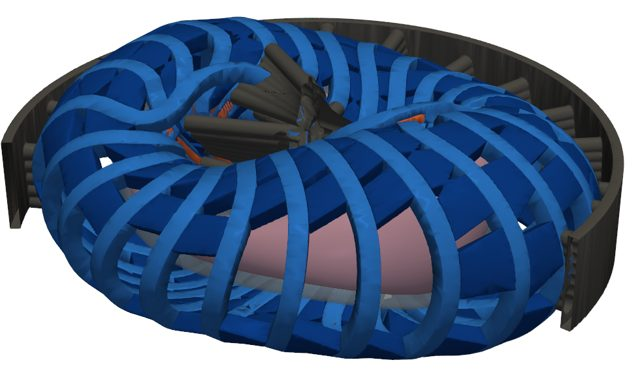
\includegraphics[width=\linewidth]{bilder/katalog/0000_en.jpg}\par\scriptsize \begin{tabular}{@{}l@{\,}r@{\quad}l@{\,}r@{}}coils & 24 & $\sigma_{99}$ & \num{840} MPa \\conn./pair & 10 & max. & \num{3425} MPa \\$E_V$ & \num{70} GPa & strain & \num{0.42} \% \\distance & \num{0.18} & $B\cdot n$ & \num{1.98} ‰ \\steel & \num{23} kt & clear. & \num{1.44} m \\\end{tabular}\par violated: σ99 steel 1.4429, winding-pack strain. PicoGK: no overlap.\end{minipage}\hfill
\begin{minipage}[t]{0.47\linewidth}\textbf{0001} \hfill \num{-191}\,\%\par 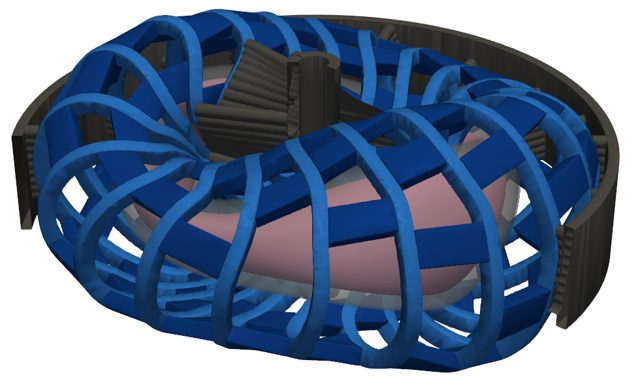
\includegraphics[width=\linewidth]{bilder/katalog/0001_en.jpg}\par\scriptsize \begin{tabular}{@{}l@{\,}r@{\quad}l@{\,}r@{}}coils & 20 & $\sigma_{99}$ & \num{1456} MPa \\conn./pair & 7 & max. & \num{3851} MPa \\$E_V$ & \num{135} GPa & strain & \num{0.60} \% \\distance & \num{0.24} & $B\cdot n$ & \num{1.53} ‰ \\steel & \num{12} kt & clear. & \num{2.00} m \\\end{tabular}\par violated: σ99 steel 1.4429, winding-pack strain. PicoGK: no overlap.\end{minipage}\par\vspace{6pt}
\begin{minipage}[t]{0.47\linewidth}\textbf{0002} \hfill \num{-844}\,\%\par 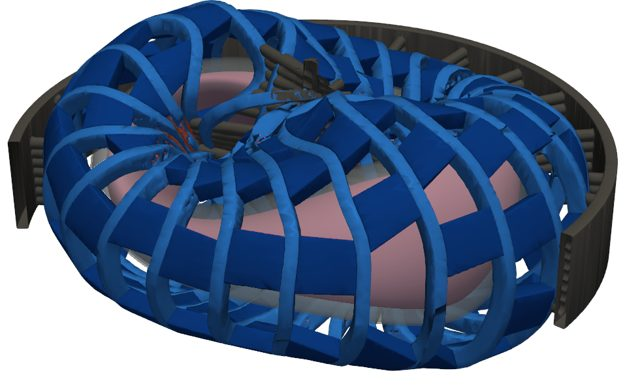
\includegraphics[width=\linewidth]{bilder/katalog/0002_en.jpg}\par\scriptsize \begin{tabular}{@{}l@{\,}r@{\quad}l@{\,}r@{}}coils & 24 & $\sigma_{99}$ & \num{4721} MPa \\conn./pair & 8 & max. & \num{13357} MPa \\$E_V$ & \num{25} GPa & strain & \num{2.01} \% \\distance & \num{0.30} & $B\cdot n$ & \num{3.67} ‰ \\steel & \num{13} kt & clear. & \num{2.39} m \\\end{tabular}\par violated: σ99 steel 1.4429, winding-pack strain, field error B·n. PicoGK: no overlap.\end{minipage}\hfill
\begin{minipage}[t]{0.47\linewidth}\textbf{0003} \hfill \num{-216}\,\%\par 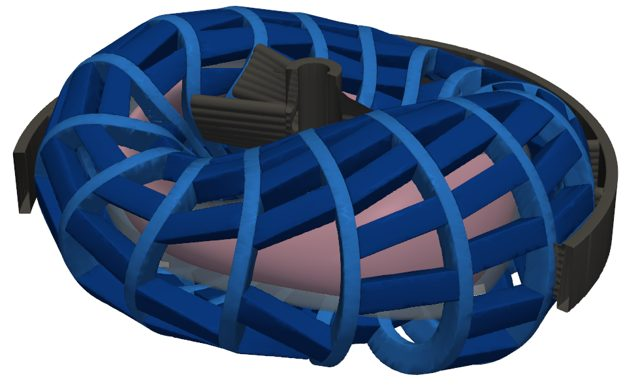
\includegraphics[width=\linewidth]{bilder/katalog/0003_en.jpg}\par\scriptsize \begin{tabular}{@{}l@{\,}r@{\quad}l@{\,}r@{}}coils & 16 & $\sigma_{99}$ & \num{617} MPa \\conn./pair & 12 & max. & \num{1361} MPa \\$E_V$ & \num{142} GPa & strain & \num{0.26} \% \\distance & \num{0.20} & $B\cdot n$ & \num{9.48} ‰ \\steel & \num{20} kt & clear. & \num{1.40} m \\\end{tabular}\par violated: σ99 steel 1.4429, field error B·n. PicoGK: no overlap.\end{minipage}\par\vspace{6pt}
\clearpage
\begin{minipage}[t]{0.47\linewidth}\textbf{0004} \hfill \num{-12}\,\%\par 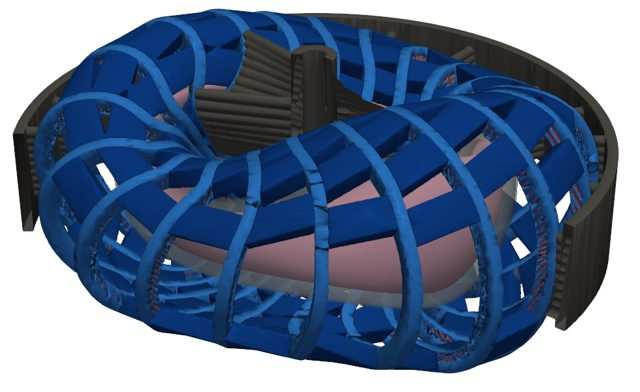
\includegraphics[width=\linewidth]{bilder/katalog/0004_en.jpg}\par\scriptsize \begin{tabular}{@{}l@{\,}r@{\quad}l@{\,}r@{}}coils & 20 & $\sigma_{99}$ & \num{558} MPa \\conn./pair & 10 & max. & \num{1085} MPa \\$E_V$ & \num{148} GPa & strain & \num{0.26} \% \\distance & \num{0.19} & $B\cdot n$ & \num{1.81} ‰ \\steel & \num{19} kt & clear. & \num{1.54} m \\\end{tabular}\par violated: σ99 steel 1.4429. PicoGK: no overlap.\end{minipage}\hfill
\begin{minipage}[t]{0.47\linewidth}\textbf{0005} \hfill \num{-69}\,\%\par 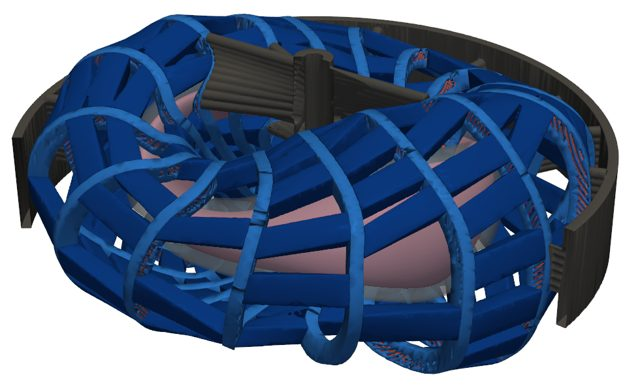
\includegraphics[width=\linewidth]{bilder/katalog/0005_en.jpg}\par\scriptsize \begin{tabular}{@{}l@{\,}r@{\quad}l@{\,}r@{}}coils & 16 & $\sigma_{99}$ & \num{844} MPa \\conn./pair & 13 & max. & \num{1847} MPa \\$E_V$ & \num{114} GPa & strain & \num{0.35} \% \\distance & \num{0.15} & $B\cdot n$ & \num{2.40} ‰ \\steel & \num{23} kt & clear. & \num{1.26} m \\\end{tabular}\par violated: σ99 steel 1.4429, winding-pack strain, neutron fluence. PicoGK: no overlap.\end{minipage}\par\vspace{6pt}
\begin{minipage}[t]{0.47\linewidth}\textbf{0006} \hfill \num{-1480}\,\%\par 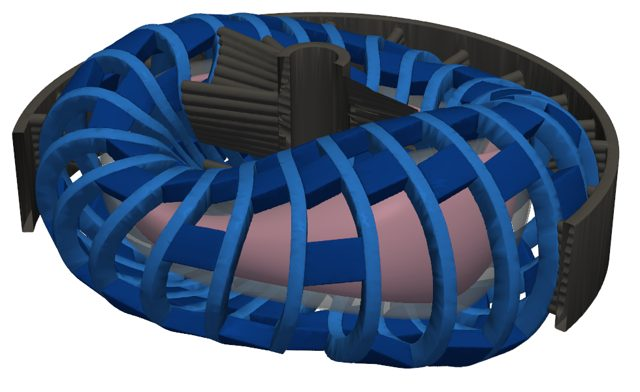
\includegraphics[width=\linewidth]{bilder/katalog/0006_en.jpg}\par\scriptsize \begin{tabular}{@{}l@{\,}r@{\quad}l@{\,}r@{}}coils & 24 & $\sigma_{99}$ & \num{536} MPa \\conn./pair & 6 & max. & \num{1222} MPa \\$E_V$ & \num{78} GPa & strain & \num{0.22} \% \\distance & \num{0.12} & $B\cdot n$ & \num{1.77} ‰ \\steel & \num{14} kt & clear. & \num{0.99} m \\\end{tabular}\par violated: σ99 steel 1.4429, package space, nuclear heating, neutron fluence. PicoGK: no overlap.\end{minipage}\hfill
\begin{minipage}[t]{0.47\linewidth}\textbf{0007} \hfill \num{-231}\,\%\par 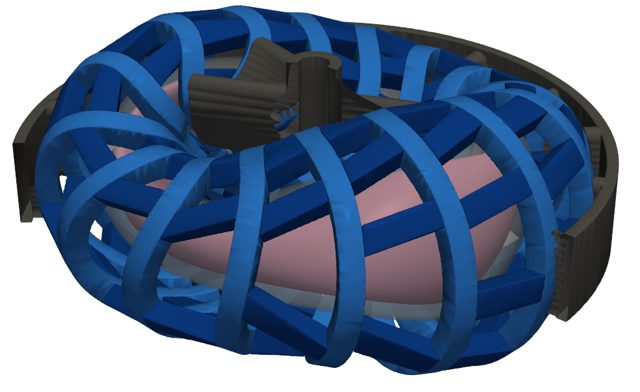
\includegraphics[width=\linewidth]{bilder/katalog/0007_en.jpg}\par\scriptsize \begin{tabular}{@{}l@{\,}r@{\quad}l@{\,}r@{}}coils & 16 & $\sigma_{99}$ & \num{870} MPa \\conn./pair & 8 & max. & \num{3574} MPa \\$E_V$ & \num{88} GPa & strain & \num{0.42} \% \\distance & \num{0.16} & $B\cdot n$ & \num{9.92} ‰ \\steel & \num{17} kt & clear. & \num{1.60} m \\\end{tabular}\par violated: σ99 steel 1.4429, winding-pack strain, field error B·n. PicoGK: no overlap.\end{minipage}\par\vspace{6pt}
\clearpage
\begin{minipage}[t]{0.47\linewidth}\textbf{0008} \hfill \num{27}\,\%\par 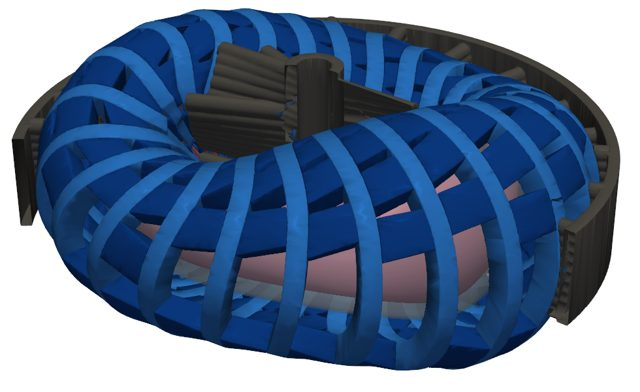
\includegraphics[width=\linewidth]{bilder/katalog/0008_en.jpg}\par\scriptsize \begin{tabular}{@{}l@{\,}r@{\quad}l@{\,}r@{}}coils & 24 & $\sigma_{99}$ & \num{305} MPa \\conn./pair & 11 & max. & \num{1695} MPa \\$E_V$ & \num{142} GPa & strain & \num{0.17} \% \\distance & \num{0.21} & $B\cdot n$ & \num{2.20} ‰ \\steel & \num{26} kt & clear. & \num{1.48} m \\\end{tabular}\par \textbf{admissible}. PicoGK: no overlap.\end{minipage}\hfill
\begin{minipage}[t]{0.47\linewidth}\textbf{0009} \hfill \num{-132}\,\%\par 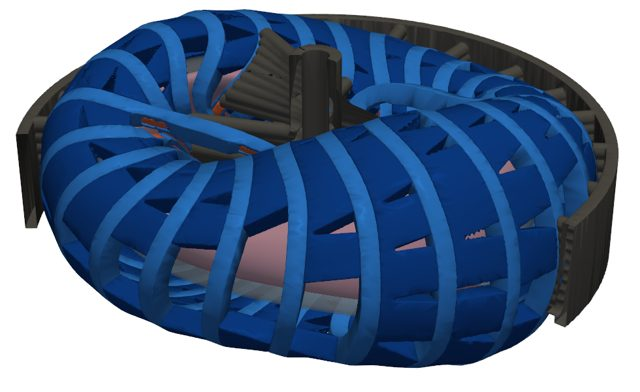
\includegraphics[width=\linewidth]{bilder/katalog/0009_en.jpg}\par\scriptsize \begin{tabular}{@{}l@{\,}r@{\quad}l@{\,}r@{}}coils & 24 & $\sigma_{99}$ & \num{1159} MPa \\conn./pair & 13 & max. & \num{9216} MPa \\$E_V$ & \num{145} GPa & strain & \num{0.62} \% \\distance & \num{0.23} & $B\cdot n$ & \num{1.50} ‰ \\steel & \num{24} kt & clear. & \num{1.55} m \\\end{tabular}\par violated: σ99 steel 1.4429, winding-pack strain. PicoGK: no overlap.\end{minipage}\par\vspace{6pt}
\begin{minipage}[t]{0.47\linewidth}\textbf{0010} \hfill \num{-176}\,\%\par 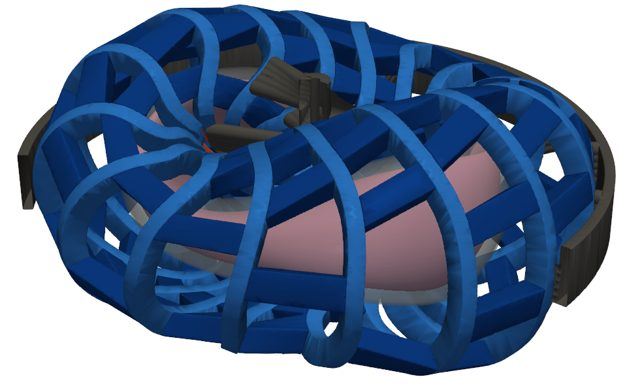
\includegraphics[width=\linewidth]{bilder/katalog/0010_en.jpg}\par\scriptsize \begin{tabular}{@{}l@{\,}r@{\quad}l@{\,}r@{}}coils & 16 & $\sigma_{99}$ & \num{1381} MPa \\conn./pair & 8 & max. & \num{8739} MPa \\$E_V$ & \num{149} GPa & strain & \num{0.63} \% \\distance & \num{0.27} & $B\cdot n$ & \num{2.80} ‰ \\steel & \num{21} kt & clear. & \num{1.93} m \\\end{tabular}\par violated: σ99 steel 1.4429, winding-pack strain. PicoGK: no overlap.\end{minipage}\hfill
\begin{minipage}[t]{0.47\linewidth}\textbf{0011} \hfill \num{-519}\,\%\par 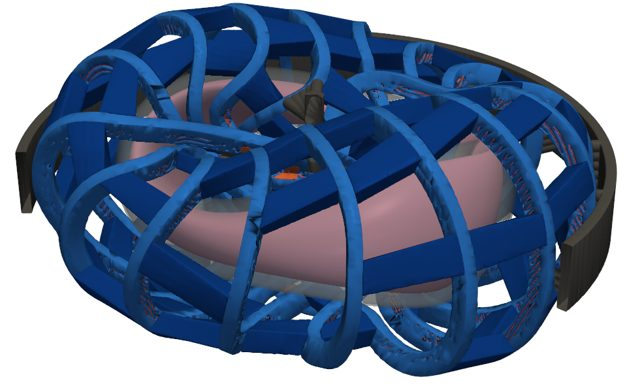
\includegraphics[width=\linewidth]{bilder/katalog/0011_en.jpg}\par\scriptsize \begin{tabular}{@{}l@{\,}r@{\quad}l@{\,}r@{}}coils & 16 & $\sigma_{99}$ & \num{3096} MPa \\conn./pair & 7 & max. & \num{19166} MPa \\$E_V$ & \num{42} GPa & strain & \num{1.50} \% \\distance & \num{0.18} & $B\cdot n$ & \num{3.25} ‰ \\steel & \num{14} kt & clear. & \num{1.80} m \\\end{tabular}\par violated: σ99 steel 1.4429, winding-pack strain, field error B·n. PicoGK: no overlap.\end{minipage}\par\vspace{6pt}
\clearpage
\begin{minipage}[t]{0.47\linewidth}\textbf{0012} \hfill \num{-139}\,\%\par 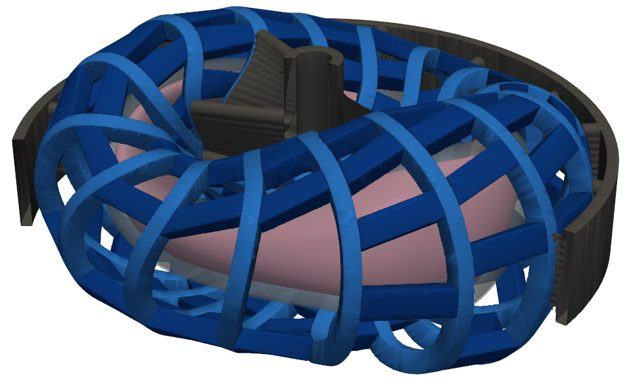
\includegraphics[width=\linewidth]{bilder/katalog/0012_en.jpg}\par\scriptsize \begin{tabular}{@{}l@{\,}r@{\quad}l@{\,}r@{}}coils & 16 & $\sigma_{99}$ & \num{999} MPa \\conn./pair & 9 & max. & \num{2952} MPa \\$E_V$ & \num{50} GPa & strain & \num{0.40} \% \\distance & \num{0.21} & $B\cdot n$ & \num{7.17} ‰ \\steel & \num{13} kt & clear. & \num{1.68} m \\\end{tabular}\par violated: σ99 steel 1.4429, winding-pack strain, field error B·n. PicoGK: no overlap.\end{minipage}\hfill
\begin{minipage}[t]{0.47\linewidth}\textbf{0013} \hfill \num{-55}\,\%\par 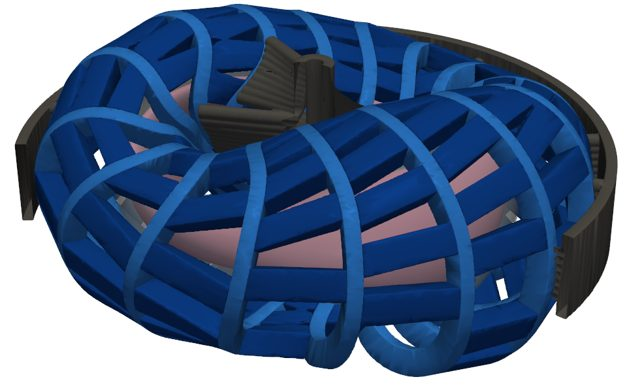
\includegraphics[width=\linewidth]{bilder/katalog/0013_en.jpg}\par\scriptsize \begin{tabular}{@{}l@{\,}r@{\quad}l@{\,}r@{}}coils & 16 & $\sigma_{99}$ & \num{773} MPa \\conn./pair & 14 & max. & \num{1718} MPa \\$E_V$ & \num{103} GPa & strain & \num{0.34} \% \\distance & \num{0.13} & $B\cdot n$ & \num{4.32} ‰ \\steel & \num{25} kt & clear. & \num{1.63} m \\\end{tabular}\par violated: σ99 steel 1.4429, winding-pack strain, field error B·n. PicoGK: no overlap.\end{minipage}\par\vspace{6pt}
\begin{minipage}[t]{0.47\linewidth}\textbf{0014} \hfill \num{25}\,\%\par 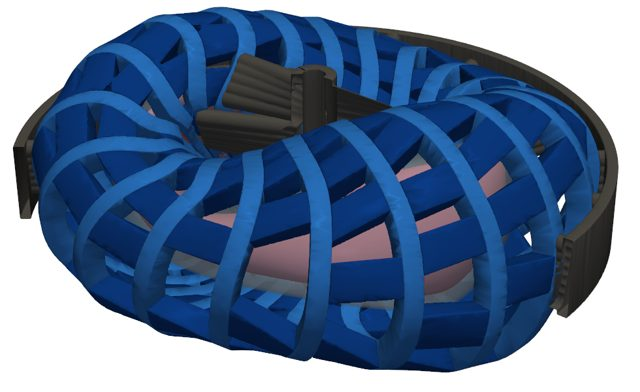
\includegraphics[width=\linewidth]{bilder/katalog/0014_en.jpg}\par\scriptsize \begin{tabular}{@{}l@{\,}r@{\quad}l@{\,}r@{}}coils & 20 & $\sigma_{99}$ & \num{377} MPa \\conn./pair & 11 & max. & \num{1419} MPa \\$E_V$ & \num{196} GPa & strain & \num{0.21} \% \\distance & \num{0.23} & $B\cdot n$ & \num{2.21} ‰ \\steel & \num{28} kt & clear. & \num{1.65} m \\\end{tabular}\par \textbf{admissible}. PicoGK: no overlap.\end{minipage}\hfill
\begin{minipage}[t]{0.47\linewidth}\textbf{0015} \hfill \num{-628}\,\%\par 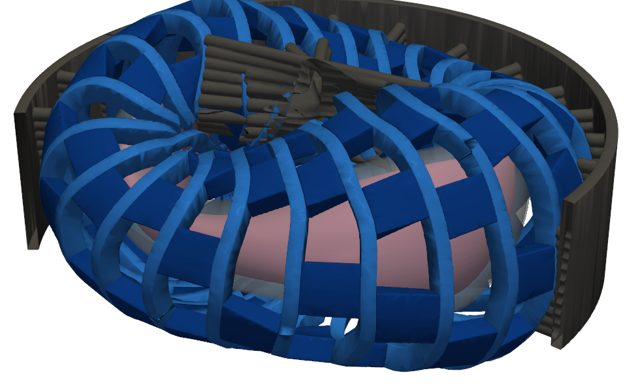
\includegraphics[width=\linewidth]{bilder/katalog/0015_en.jpg}\par\scriptsize \begin{tabular}{@{}l@{\,}r@{\quad}l@{\,}r@{}}coils & 24 & $\sigma_{99}$ & \num{3586} MPa \\conn./pair & 7 & max. & \num{30683} MPa \\$E_V$ & \num{168} GPa & strain & \num{2.18} \% \\distance & \num{0.29} & $B\cdot n$ & \num{1.12} ‰ \\steel & \num{18} kt & clear. & \num{2.48} m \\\end{tabular}\par violated: σ99 steel 1.4429, winding-pack strain. PicoGK: no overlap.\end{minipage}\par\vspace{6pt}
\clearpage
\begin{minipage}[t]{0.47\linewidth}\textbf{0016} \hfill \num{-600}\,\%\par 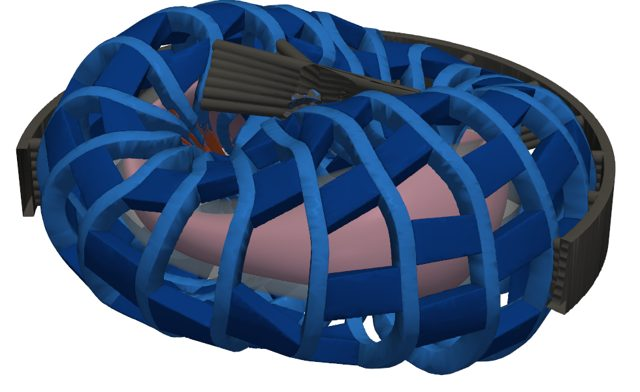
\includegraphics[width=\linewidth]{bilder/katalog/0016_en.jpg}\par\scriptsize \begin{tabular}{@{}l@{\,}r@{\quad}l@{\,}r@{}}coils & 20 & $\sigma_{99}$ & \num{3499} MPa \\conn./pair & 8 & max. & \num{15129} MPa \\$E_V$ & \num{172} GPa & strain & \num{1.95} \% \\distance & \num{0.29} & $B\cdot n$ & \num{2.24} ‰ \\steel & \num{19} kt & clear. & \num{2.42} m \\\end{tabular}\par violated: σ99 steel 1.4429, winding-pack strain. PicoGK: no overlap.\end{minipage}\hfill
\begin{minipage}[t]{0.47\linewidth}\textbf{0017} \hfill \num{20}\,\%\par 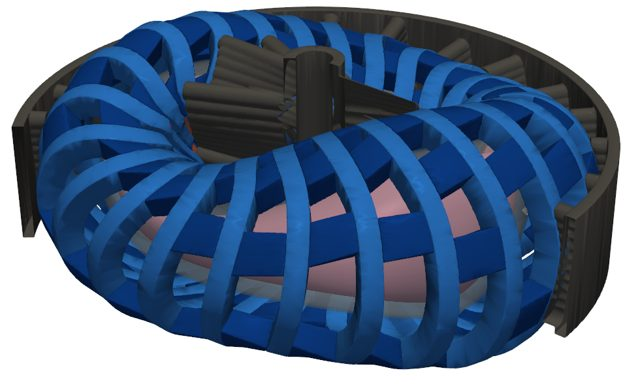
\includegraphics[width=\linewidth]{bilder/katalog/0017_en.jpg}\par\scriptsize \begin{tabular}{@{}l@{\,}r@{\quad}l@{\,}r@{}}coils & 24 & $\sigma_{99}$ & \num{389} MPa \\conn./pair & 7 & max. & \num{1721} MPa \\$E_V$ & \num{29} GPa & strain & \num{0.20} \% \\distance & \num{0.22} & $B\cdot n$ & \num{1.66} ‰ \\steel & \num{23} kt & clear. & \num{1.30} m \\\end{tabular}\par \textbf{admissible}. PicoGK: no overlap.\end{minipage}\par\vspace{6pt}
\begin{minipage}[t]{0.47\linewidth}\textbf{0018}$^\ast$ \hfill \num{-99}\,\%\par 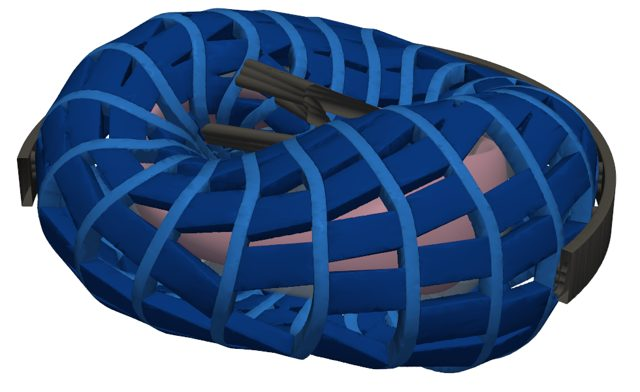
\includegraphics[width=\linewidth]{bilder/katalog/0018_en.jpg}\par\scriptsize \begin{tabular}{@{}l@{\,}r@{\quad}l@{\,}r@{}}coils & 20 & $\sigma_{99}$ & \num{996} MPa \\conn./pair & 14 & max. & \num{4566} MPa \\$E_V$ & \num{26} GPa & strain & \num{0.44} \% \\distance & \num{0.25} & $B\cdot n$ & \num{1.43} ‰ \\steel & \num{24} kt & clear. & \num{2.08} m \\\end{tabular}\par violated: σ99 steel 1.4429, winding-pack strain. PicoGK: no overlap.\end{minipage}\hfill
\begin{minipage}[t]{0.47\linewidth}\textbf{0019} \hfill \num{-338}\,\%\par 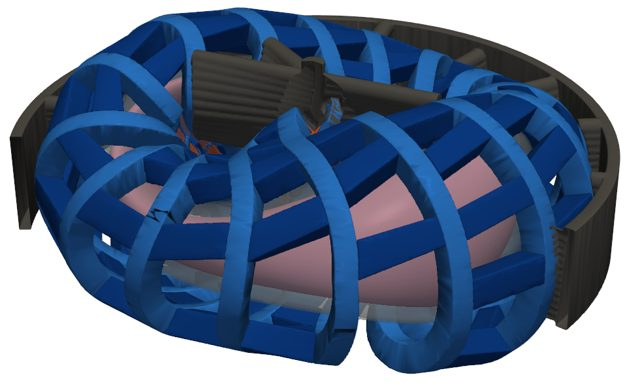
\includegraphics[width=\linewidth]{bilder/katalog/0019_en.jpg}\par\scriptsize \begin{tabular}{@{}l@{\,}r@{\quad}l@{\,}r@{}}coils & 16 & $\sigma_{99}$ & \num{1571} MPa \\conn./pair & 9 & max. & \num{14989} MPa \\$E_V$ & \num{24} GPa & strain & \num{0.96} \% \\distance & \num{0.25} & $B\cdot n$ & \num{13.15} ‰ \\steel & \num{17} kt & clear. & \num{1.93} m \\\end{tabular}\par violated: σ99 steel 1.4429, winding-pack strain, field error B·n. PicoGK: no overlap.\end{minipage}\par\vspace{6pt}
\clearpage
\begin{minipage}[t]{0.47\linewidth}\textbf{0020} \hfill \num{-173}\,\%\par 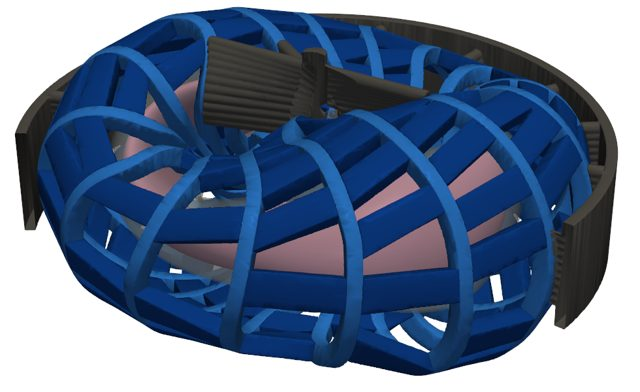
\includegraphics[width=\linewidth]{bilder/katalog/0020_en.jpg}\par\scriptsize \begin{tabular}{@{}l@{\,}r@{\quad}l@{\,}r@{}}coils & 16 & $\sigma_{99}$ & \num{1363} MPa \\conn./pair & 14 & max. & \num{6952} MPa \\$E_V$ & \num{137} GPa & strain & \num{0.55} \% \\distance & \num{0.24} & $B\cdot n$ & \num{3.21} ‰ \\steel & \num{17} kt & clear. & \num{1.78} m \\\end{tabular}\par violated: σ99 steel 1.4429, winding-pack strain, field error B·n. PicoGK: no overlap.\end{minipage}\hfill
\begin{minipage}[t]{0.47\linewidth}\textbf{0021} \hfill \num{-4948}\,\%\par 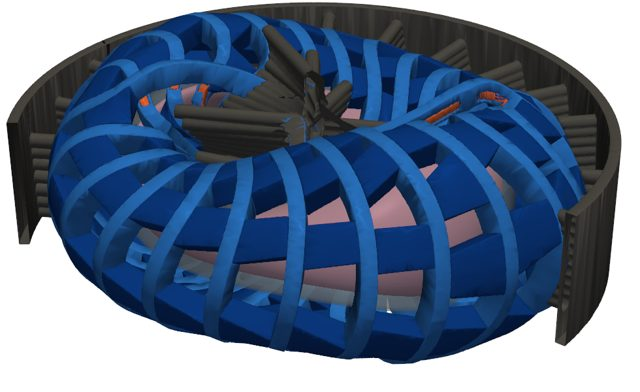
\includegraphics[width=\linewidth]{bilder/katalog/0021_en.jpg}\par\scriptsize \begin{tabular}{@{}l@{\,}r@{\quad}l@{\,}r@{}}coils & 24 & $\sigma_{99}$ & \num{558} MPa \\conn./pair & 8 & max. & \num{4173} MPa \\$E_V$ & \num{138} GPa & strain & \num{0.29} \% \\distance & \num{0.16} & $B\cdot n$ & \num{2.26} ‰ \\steel & \num{26} kt & clear. & \num{0.87} m \\\end{tabular}\par violated: σ99 steel 1.4429, package space, nuclear heating, neutron fluence. PicoGK: overlap!\end{minipage}\par\vspace{6pt}
\begin{minipage}[t]{0.47\linewidth}\textbf{0022} \hfill \num{-20}\,\%\par 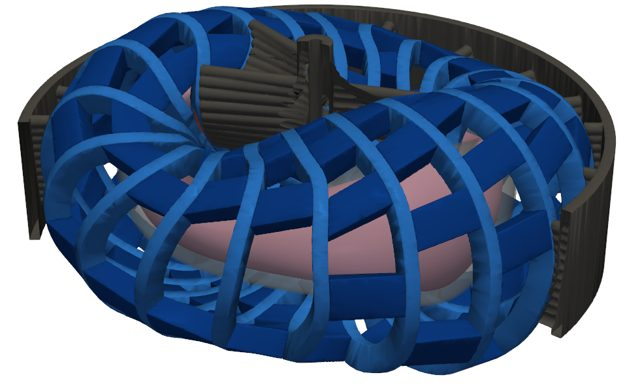
\includegraphics[width=\linewidth]{bilder/katalog/0022_en.jpg}\par\scriptsize \begin{tabular}{@{}l@{\,}r@{\quad}l@{\,}r@{}}coils & 20 & $\sigma_{99}$ & \num{600} MPa \\conn./pair & 8 & max. & \num{2183} MPa \\$E_V$ & \num{37} GPa & strain & \num{0.26} \% \\distance & \num{0.23} & $B\cdot n$ & \num{0.70} ‰ \\steel & \num{24} kt & clear. & \num{1.57} m \\\end{tabular}\par violated: σ99 steel 1.4429. PicoGK: no overlap.\end{minipage}\hfill
\begin{minipage}[t]{0.47\linewidth}\textbf{0023} \hfill \num{-276}\,\%\par 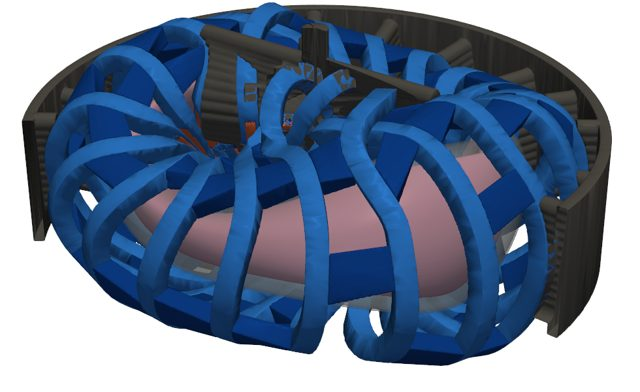
\includegraphics[width=\linewidth]{bilder/katalog/0023_en.jpg}\par\scriptsize \begin{tabular}{@{}l@{\,}r@{\quad}l@{\,}r@{}}coils & 20 & $\sigma_{99}$ & \num{1864} MPa \\conn./pair & 6 & max. & \num{10858} MPa \\$E_V$ & \num{156} GPa & strain & \num{1.13} \% \\distance & \num{0.28} & $B\cdot n$ & \num{2.89} ‰ \\steel & \num{15} kt & clear. & \num{2.06} m \\\end{tabular}\par violated: σ99 steel 1.4429, winding-pack strain. PicoGK: no overlap.\end{minipage}\par\vspace{6pt}
\clearpage
\begin{minipage}[t]{0.47\linewidth}\textbf{0024} \hfill \num{-257}\,\%\par 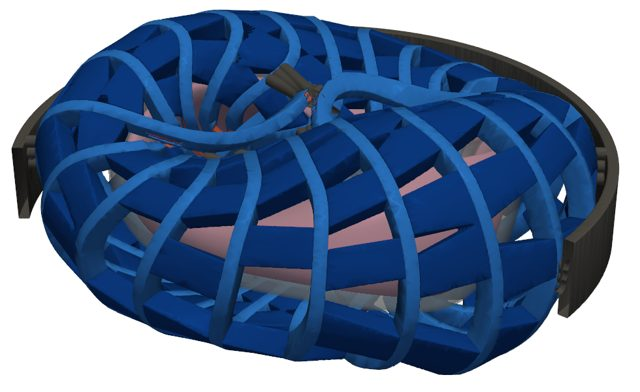
\includegraphics[width=\linewidth]{bilder/katalog/0024_en.jpg}\par\scriptsize \begin{tabular}{@{}l@{\,}r@{\quad}l@{\,}r@{}}coils & 20 & $\sigma_{99}$ & \num{1787} MPa \\conn./pair & 11 & max. & \num{7614} MPa \\$E_V$ & \num{24} GPa & strain & \num{0.85} \% \\distance & \num{0.26} & $B\cdot n$ & \num{1.55} ‰ \\steel & \num{24} kt & clear. & \num{1.82} m \\\end{tabular}\par violated: σ99 steel 1.4429, winding-pack strain. PicoGK: no overlap.\end{minipage}\hfill
\begin{minipage}[t]{0.47\linewidth}\textbf{0025} \hfill \num{-102}\,\%\par 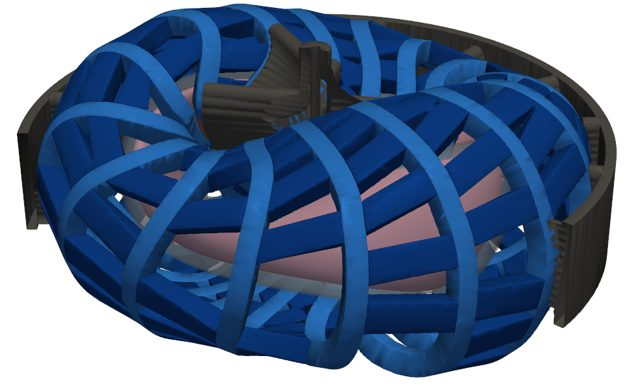
\includegraphics[width=\linewidth]{bilder/katalog/0025_en.jpg}\par\scriptsize \begin{tabular}{@{}l@{\,}r@{\quad}l@{\,}r@{}}coils & 16 & $\sigma_{99}$ & \num{1010} MPa \\conn./pair & 14 & max. & \num{9842} MPa \\$E_V$ & \num{41} GPa & strain & \num{0.50} \% \\distance & \num{0.18} & $B\cdot n$ & \num{1.94} ‰ \\steel & \num{26} kt & clear. & \num{1.88} m \\\end{tabular}\par violated: σ99 steel 1.4429, winding-pack strain. PicoGK: no overlap.\end{minipage}\par\vspace{6pt}
\begin{minipage}[t]{0.47\linewidth}\textbf{0026} \hfill \num{-62}\,\%\par 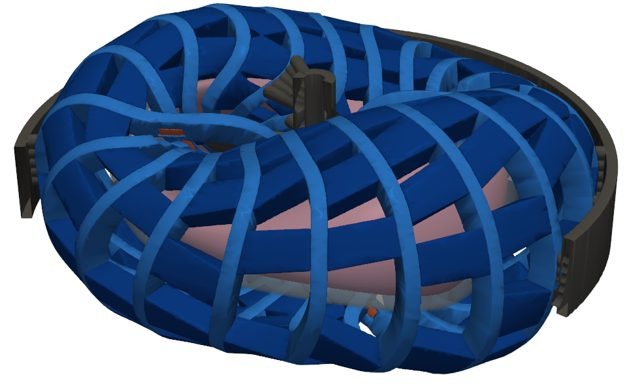
\includegraphics[width=\linewidth]{bilder/katalog/0026_en.jpg}\par\scriptsize \begin{tabular}{@{}l@{\,}r@{\quad}l@{\,}r@{}}coils & 20 & $\sigma_{99}$ & \num{809} MPa \\conn./pair & 11 & max. & \num{2253} MPa \\$E_V$ & \num{79} GPa & strain & \num{0.38} \% \\distance & \num{0.19} & $B\cdot n$ & \num{1.43} ‰ \\steel & \num{29} kt & clear. & \num{1.41} m \\\end{tabular}\par violated: σ99 steel 1.4429, winding-pack strain. PicoGK: no overlap.\end{minipage}\hfill
\begin{minipage}[t]{0.47\linewidth}\textbf{0027} \hfill \num{-316}\,\%\par 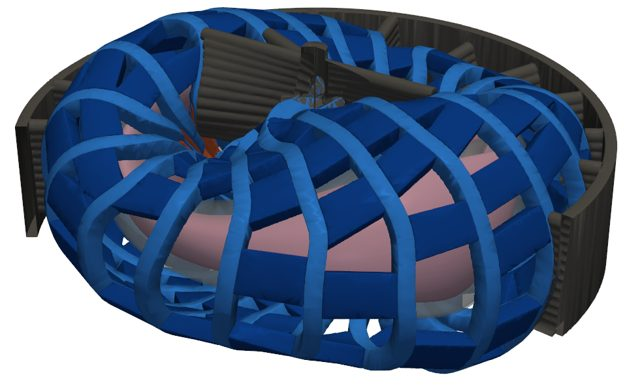
\includegraphics[width=\linewidth]{bilder/katalog/0027_en.jpg}\par\scriptsize \begin{tabular}{@{}l@{\,}r@{\quad}l@{\,}r@{}}coils & 20 & $\sigma_{99}$ & \num{2080} MPa \\conn./pair & 10 & max. & \num{10143} MPa \\$E_V$ & \num{171} GPa & strain & \num{1.02} \% \\distance & \num{0.28} & $B\cdot n$ & \num{2.25} ‰ \\steel & \num{16} kt & clear. & \num{2.18} m \\\end{tabular}\par violated: σ99 steel 1.4429, winding-pack strain. PicoGK: no overlap.\end{minipage}\par\vspace{6pt}
\clearpage
\begin{minipage}[t]{0.47\linewidth}\textbf{0028} \hfill \num{-78}\,\%\par 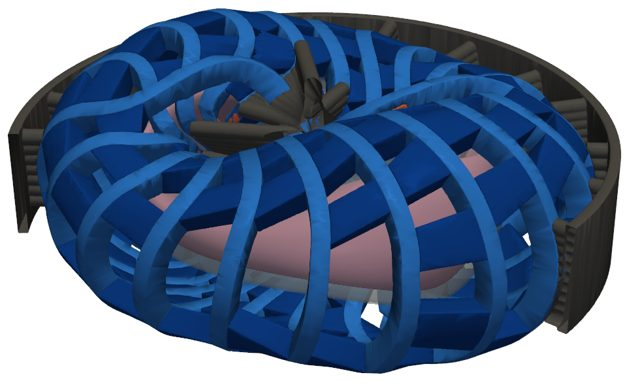
\includegraphics[width=\linewidth]{bilder/katalog/0028_en.jpg}\par\scriptsize \begin{tabular}{@{}l@{\,}r@{\quad}l@{\,}r@{}}coils & 20 & $\sigma_{99}$ & \num{888} MPa \\conn./pair & 9 & max. & \num{3682} MPa \\$E_V$ & \num{22} GPa & strain & \num{0.40} \% \\distance & \num{0.17} & $B\cdot n$ & \num{1.45} ‰ \\steel & \num{30} kt & clear. & \num{1.33} m \\\end{tabular}\par violated: σ99 steel 1.4429, winding-pack strain. PicoGK: no overlap.\end{minipage}\hfill
\begin{minipage}[t]{0.47\linewidth}\textbf{0029} \hfill \num{-361}\,\%\par 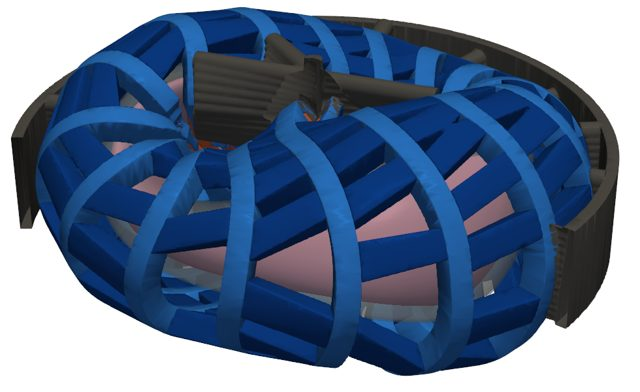
\includegraphics[width=\linewidth]{bilder/katalog/0029_en.jpg}\par\scriptsize \begin{tabular}{@{}l@{\,}r@{\quad}l@{\,}r@{}}coils & 16 & $\sigma_{99}$ & \num{1975} MPa \\conn./pair & 13 & max. & \num{34584} MPa \\$E_V$ & \num{27} GPa & strain & \num{1.38} \% \\distance & \num{0.29} & $B\cdot n$ & \num{10.34} ‰ \\steel & \num{22} kt & clear. & \num{2.35} m \\\end{tabular}\par violated: σ99 steel 1.4429, winding-pack strain, field error B·n. PicoGK: no overlap.\end{minipage}\par\vspace{6pt}
\begin{minipage}[t]{0.47\linewidth}\textbf{0031} \hfill \num{-222}\,\%\par 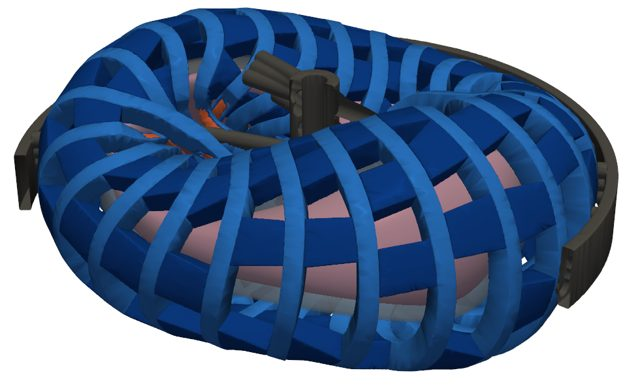
\includegraphics[width=\linewidth]{bilder/katalog/0031_en.jpg}\par\scriptsize \begin{tabular}{@{}l@{\,}r@{\quad}l@{\,}r@{}}coils & 24 & $\sigma_{99}$ & \num{1514} MPa \\conn./pair & 8 & max. & \num{8426} MPa \\$E_V$ & \num{190} GPa & strain & \num{0.97} \% \\distance & \num{0.24} & $B\cdot n$ & \num{1.99} ‰ \\steel & \num{21} kt & clear. & \num{1.84} m \\\end{tabular}\par violated: σ99 steel 1.4429, winding-pack strain. PicoGK: no overlap.\end{minipage}\hfill
\begin{minipage}[t]{0.47\linewidth}\textbf{0032} \hfill \num{-123}\,\%\par 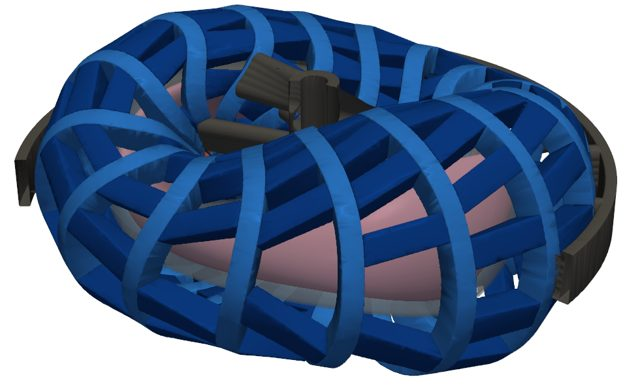
\includegraphics[width=\linewidth]{bilder/katalog/0032_en.jpg}\par\scriptsize \begin{tabular}{@{}l@{\,}r@{\quad}l@{\,}r@{}}coils & 16 & $\sigma_{99}$ & \num{777} MPa \\conn./pair & 12 & max. & \num{3008} MPa \\$E_V$ & \num{38} GPa & strain & \num{0.28} \% \\distance & \num{0.17} & $B\cdot n$ & \num{6.70} ‰ \\steel & \num{25} kt & clear. & \num{1.48} m \\\end{tabular}\par violated: σ99 steel 1.4429, field error B·n. PicoGK: no overlap.\end{minipage}\par\vspace{6pt}
\clearpage
\begin{minipage}[t]{0.47\linewidth}\textbf{0033} \hfill \num{-125}\,\%\par 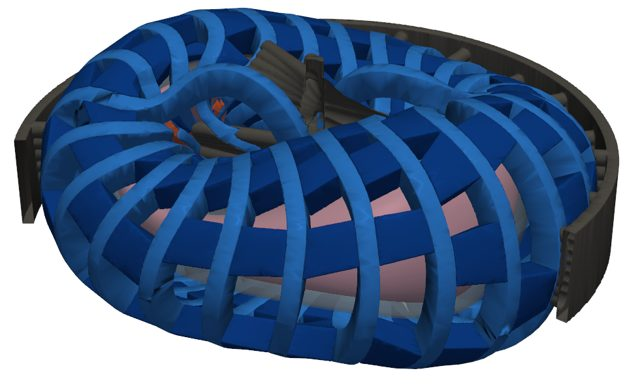
\includegraphics[width=\linewidth]{bilder/katalog/0033_en.jpg}\par\scriptsize \begin{tabular}{@{}l@{\,}r@{\quad}l@{\,}r@{}}coils & 24 & $\sigma_{99}$ & \num{1019} MPa \\conn./pair & 8 & max. & \num{4409} MPa \\$E_V$ & \num{118} GPa & strain & \num{0.68} \% \\distance & \num{0.25} & $B\cdot n$ & \num{1.78} ‰ \\steel & \num{25} kt & clear. & \num{1.56} m \\\end{tabular}\par violated: σ99 steel 1.4429, winding-pack strain. PicoGK: no overlap.\end{minipage}\hfill
\begin{minipage}[t]{0.47\linewidth}\textbf{0034} \hfill \num{-215}\,\%\par 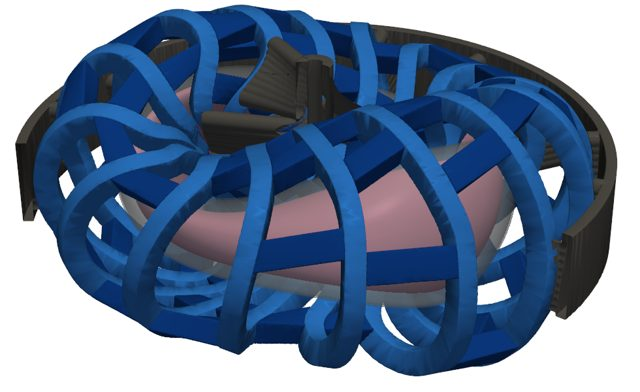
\includegraphics[width=\linewidth]{bilder/katalog/0034_en.jpg}\par\scriptsize \begin{tabular}{@{}l@{\,}r@{\quad}l@{\,}r@{}}coils & 16 & $\sigma_{99}$ & \num{1574} MPa \\conn./pair & 6 & max. & \num{4775} MPa \\$E_V$ & \num{21} GPa & strain & \num{0.56} \% \\distance & \num{0.26} & $B\cdot n$ & \num{3.08} ‰ \\steel & \num{17} kt & clear. & \num{1.96} m \\\end{tabular}\par violated: σ99 steel 1.4429, winding-pack strain, field error B·n. PicoGK: no overlap.\end{minipage}\par\vspace{6pt}
\begin{minipage}[t]{0.47\linewidth}\textbf{0035} \hfill \num{-278}\,\%\par 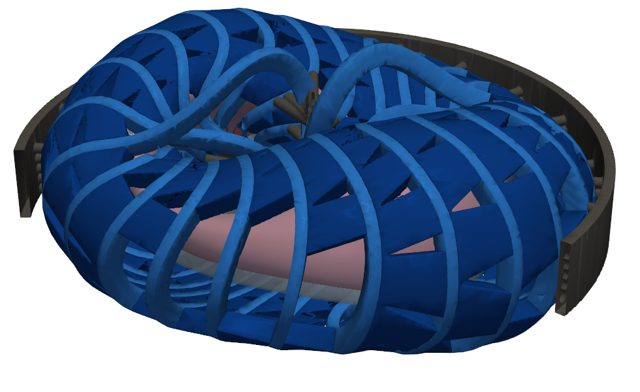
\includegraphics[width=\linewidth]{bilder/katalog/0035_en.jpg}\par\scriptsize \begin{tabular}{@{}l@{\,}r@{\quad}l@{\,}r@{}}coils & 24 & $\sigma_{99}$ & \num{1892} MPa \\conn./pair & 12 & max. & \num{5956} MPa \\$E_V$ & \num{50} GPa & strain & \num{0.83} \% \\distance & \num{0.18} & $B\cdot n$ & \num{1.23} ‰ \\steel & \num{30} kt & clear. & \num{1.31} m \\\end{tabular}\par violated: σ99 steel 1.4429, winding-pack strain. PicoGK: no overlap.\end{minipage}\hfill
\begin{minipage}[t]{0.47\linewidth}\textbf{0036} \hfill \num{-37}\,\%\par 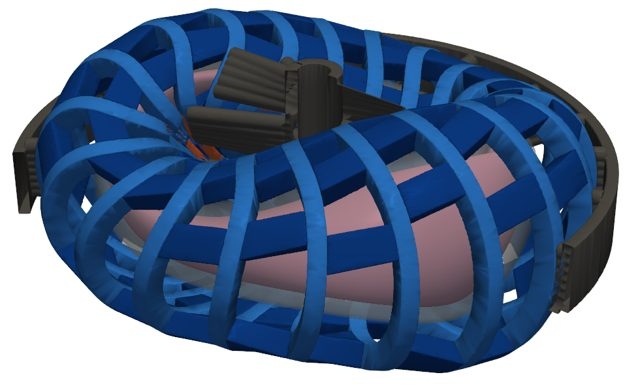
\includegraphics[width=\linewidth]{bilder/katalog/0036_en.jpg}\par\scriptsize \begin{tabular}{@{}l@{\,}r@{\quad}l@{\,}r@{}}coils & 20 & $\sigma_{99}$ & \num{683} MPa \\conn./pair & 7 & max. & \num{7457} MPa \\$E_V$ & \num{119} GPa & strain & \num{0.38} \% \\distance & \num{0.25} & $B\cdot n$ & \num{3.45} ‰ \\steel & \num{15} kt & clear. & \num{1.74} m \\\end{tabular}\par violated: σ99 steel 1.4429, winding-pack strain, field error B·n. PicoGK: no overlap.\end{minipage}\par\vspace{6pt}
\clearpage
\begin{minipage}[t]{0.47\linewidth}\textbf{0037} \hfill \num{-260}\,\%\par 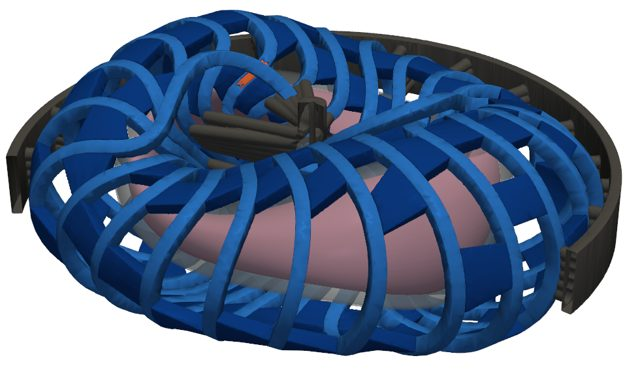
\includegraphics[width=\linewidth]{bilder/katalog/0037_en.jpg}\par\scriptsize \begin{tabular}{@{}l@{\,}r@{\quad}l@{\,}r@{}}coils & 24 & $\sigma_{99}$ & \num{1800} MPa \\conn./pair & 6 & max. & \num{4950} MPa \\$E_V$ & \num{53} GPa & strain & \num{0.66} \% \\distance & \num{0.13} & $B\cdot n$ & \num{1.33} ‰ \\steel & \num{12} kt & clear. & \num{1.43} m \\\end{tabular}\par violated: σ99 steel 1.4429, winding-pack strain. PicoGK: no overlap.\end{minipage}\hfill
\begin{minipage}[t]{0.47\linewidth}\textbf{0038} \hfill \num{-204}\,\%\par 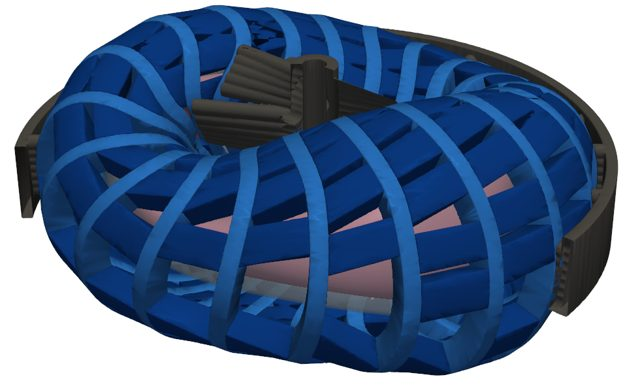
\includegraphics[width=\linewidth]{bilder/katalog/0038_en.jpg}\par\scriptsize \begin{tabular}{@{}l@{\,}r@{\quad}l@{\,}r@{}}coils & 20 & $\sigma_{99}$ & \num{525} MPa \\conn./pair & 13 & max. & \num{2561} MPa \\$E_V$ & \num{60} GPa & strain & \num{0.23} \% \\distance & \num{0.17} & $B\cdot n$ & \num{3.27} ‰ \\steel & \num{32} kt & clear. & \num{1.15} m \\\end{tabular}\par violated: σ99 steel 1.4429, neutron fluence, field error B·n. PicoGK: no overlap.\end{minipage}\par\vspace{6pt}
\begin{minipage}[t]{0.47\linewidth}\textbf{0039} \hfill \num{-210}\,\%\par 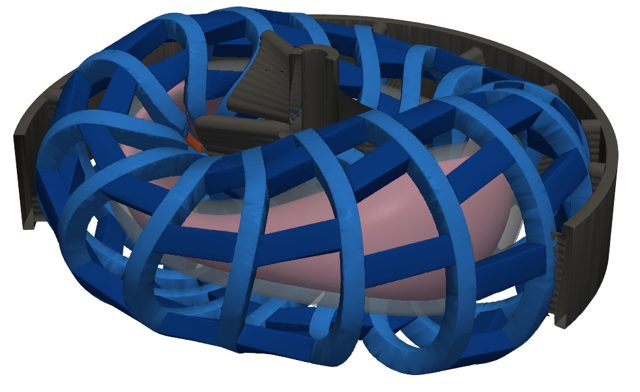
\includegraphics[width=\linewidth]{bilder/katalog/0039_en.jpg}\par\scriptsize \begin{tabular}{@{}l@{\,}r@{\quad}l@{\,}r@{}}coils & 16 & $\sigma_{99}$ & \num{1548} MPa \\conn./pair & 7 & max. & \num{6664} MPa \\$E_V$ & \num{31} GPa & strain & \num{0.70} \% \\distance & \num{0.28} & $B\cdot n$ & \num{4.38} ‰ \\steel & \num{14} kt & clear. & \num{2.05} m \\\end{tabular}\par violated: σ99 steel 1.4429, winding-pack strain, field error B·n. PicoGK: no overlap.\end{minipage}\hfill
\begin{minipage}[t]{0.47\linewidth}\textbf{0040} \hfill \num{-240}\,\%\par 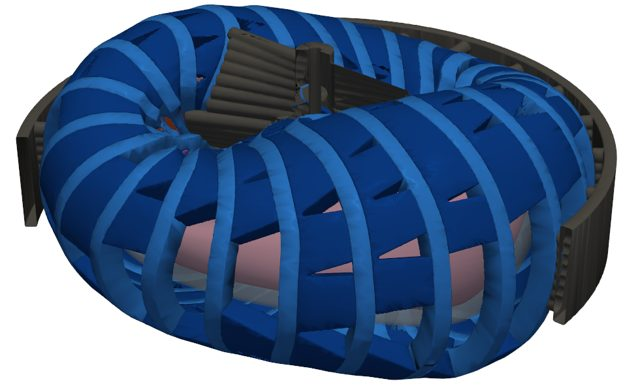
\includegraphics[width=\linewidth]{bilder/katalog/0040_en.jpg}\par\scriptsize \begin{tabular}{@{}l@{\,}r@{\quad}l@{\,}r@{}}coils & 24 & $\sigma_{99}$ & \num{1262} MPa \\conn./pair & 12 & max. & \num{9182} MPa \\$E_V$ & \num{91} GPa & strain & \num{1.02} \% \\distance & \num{0.29} & $B\cdot n$ & \num{3.84} ‰ \\steel & \num{23} kt & clear. & \num{2.41} m \\\end{tabular}\par violated: σ99 steel 1.4429, winding-pack strain, field error B·n. PicoGK: no overlap.\end{minipage}\par\vspace{6pt}
\clearpage
\begin{minipage}[t]{0.47\linewidth}\textbf{0041} \hfill \num{-69}\,\%\par 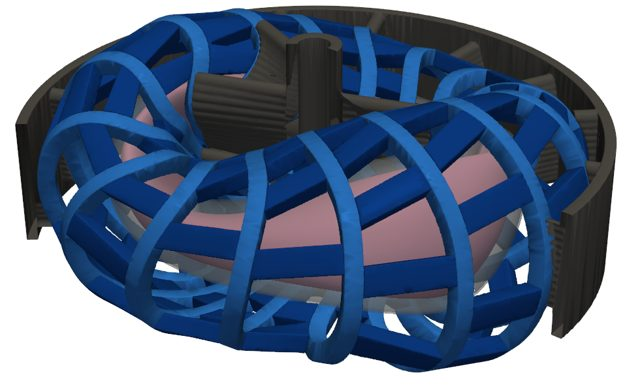
\includegraphics[width=\linewidth]{bilder/katalog/0041_en.jpg}\par\scriptsize \begin{tabular}{@{}l@{\,}r@{\quad}l@{\,}r@{}}coils & 16 & $\sigma_{99}$ & \num{843} MPa \\conn./pair & 9 & max. & \num{1629} MPa \\$E_V$ & \num{73} GPa & strain & \num{0.36} \% \\distance & \num{0.14} & $B\cdot n$ & \num{4.96} ‰ \\steel & \num{13} kt & clear. & \num{1.60} m \\\end{tabular}\par violated: σ99 steel 1.4429, winding-pack strain, field error B·n. PicoGK: no overlap.\end{minipage}\hfill
\begin{minipage}[t]{0.47\linewidth}\textbf{0042} \hfill \num{-26}\,\%\par 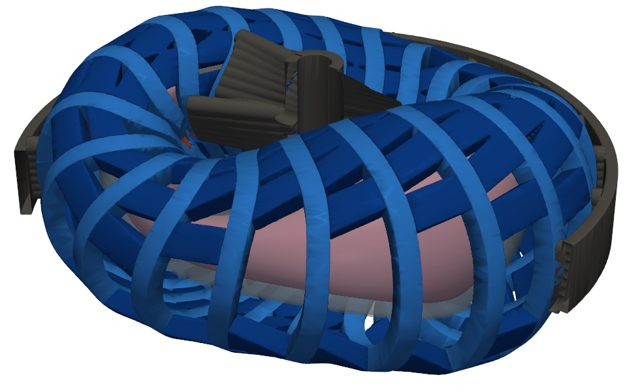
\includegraphics[width=\linewidth]{bilder/katalog/0042_en.jpg}\par\scriptsize \begin{tabular}{@{}l@{\,}r@{\quad}l@{\,}r@{}}coils & 20 & $\sigma_{99}$ & \num{632} MPa \\conn./pair & 12 & max. & \num{3962} MPa \\$E_V$ & \num{170} GPa & strain & \num{0.34} \% \\distance & \num{0.14} & $B\cdot n$ & \num{2.66} ‰ \\steel & \num{21} kt & clear. & \num{1.61} m \\\end{tabular}\par violated: σ99 steel 1.4429, winding-pack strain. PicoGK: no overlap.\end{minipage}\par\vspace{6pt}
\begin{minipage}[t]{0.47\linewidth}\textbf{0043} \hfill \num{-31}\,\%\par 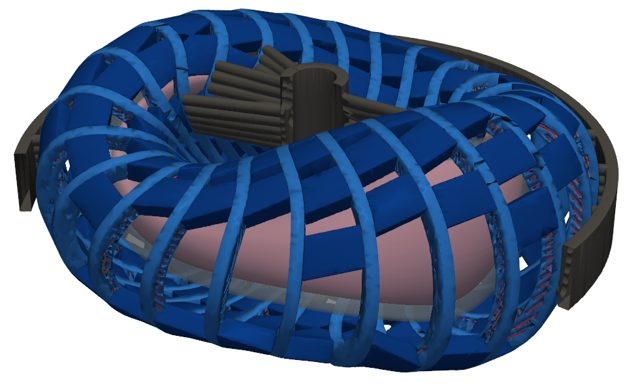
\includegraphics[width=\linewidth]{bilder/katalog/0043_en.jpg}\par\scriptsize \begin{tabular}{@{}l@{\,}r@{\quad}l@{\,}r@{}}coils & 24 & $\sigma_{99}$ & \num{653} MPa \\conn./pair & 9 & max. & \num{1208} MPa \\$E_V$ & \num{40} GPa & strain & \num{0.29} \% \\distance & \num{0.17} & $B\cdot n$ & \num{1.79} ‰ \\steel & \num{16} kt & clear. & \num{1.30} m \\\end{tabular}\par violated: σ99 steel 1.4429. PicoGK: no overlap.\end{minipage}\hfill
\begin{minipage}[t]{0.47\linewidth}\textbf{0044} \hfill \num{-8}\,\%\par 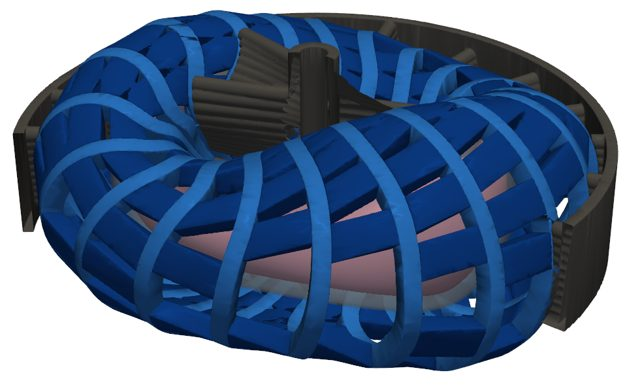
\includegraphics[width=\linewidth]{bilder/katalog/0044_en.jpg}\par\scriptsize \begin{tabular}{@{}l@{\,}r@{\quad}l@{\,}r@{}}coils & 20 & $\sigma_{99}$ & \num{540} MPa \\conn./pair & 13 & max. & \num{1583} MPa \\$E_V$ & \num{110} GPa & strain & \num{0.23} \% \\distance & \num{0.16} & $B\cdot n$ & \num{2.76} ‰ \\steel & \num{26} kt & clear. & \num{1.35} m \\\end{tabular}\par violated: σ99 steel 1.4429. PicoGK: no overlap.\end{minipage}\par\vspace{6pt}
\clearpage
\begin{minipage}[t]{0.47\linewidth}\textbf{0045} \hfill \num{-58}\,\%\par 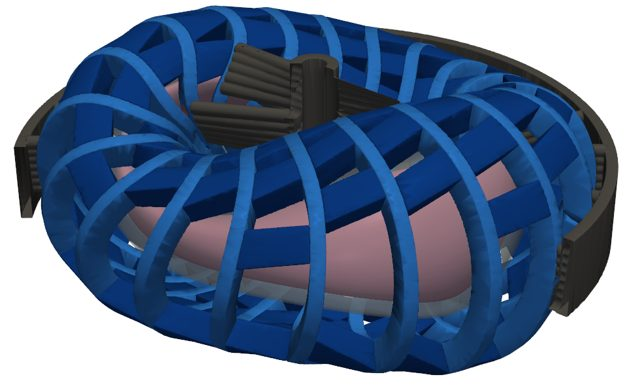
\includegraphics[width=\linewidth]{bilder/katalog/0045_en.jpg}\par\scriptsize \begin{tabular}{@{}l@{\,}r@{\quad}l@{\,}r@{}}coils & 20 & $\sigma_{99}$ & \num{600} MPa \\conn./pair & 9 & max. & \num{3060} MPa \\$E_V$ & \num{175} GPa & strain & \num{0.29} \% \\distance & \num{0.15} & $B\cdot n$ & \num{4.74} ‰ \\steel & \num{22} kt & clear. & \num{1.36} m \\\end{tabular}\par violated: σ99 steel 1.4429, field error B·n. PicoGK: no overlap.\end{minipage}\hfill
\begin{minipage}[t]{0.47\linewidth}\textbf{0046} \hfill \num{-112}\,\%\par 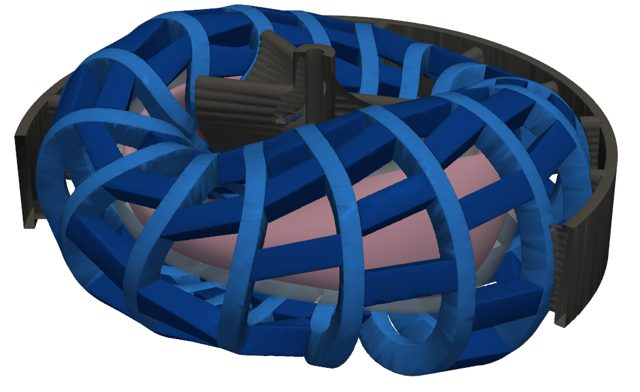
\includegraphics[width=\linewidth]{bilder/katalog/0046_en.jpg}\par\scriptsize \begin{tabular}{@{}l@{\,}r@{\quad}l@{\,}r@{}}coils & 16 & $\sigma_{99}$ & \num{619} MPa \\conn./pair & 9 & max. & \num{2502} MPa \\$E_V$ & \num{46} GPa & strain & \num{0.26} \% \\distance & \num{0.16} & $B\cdot n$ & \num{6.36} ‰ \\steel & \num{22} kt & clear. & \num{1.43} m \\\end{tabular}\par violated: σ99 steel 1.4429, field error B·n. PicoGK: no overlap.\end{minipage}\par\vspace{6pt}
\begin{minipage}[t]{0.47\linewidth}\textbf{0047} \hfill \num{-407}\,\%\par 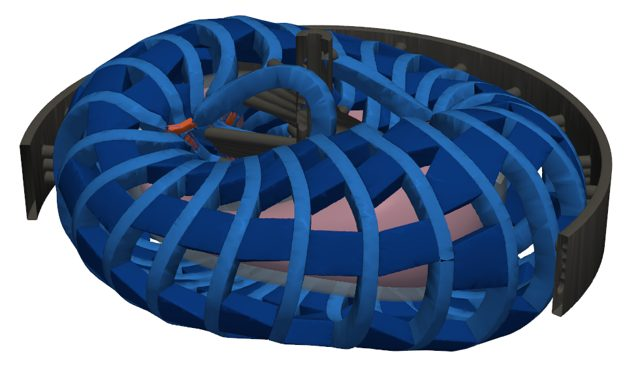
\includegraphics[width=\linewidth]{bilder/katalog/0047_en.jpg}\par\scriptsize \begin{tabular}{@{}l@{\,}r@{\quad}l@{\,}r@{}}coils & 24 & $\sigma_{99}$ & \num{983} MPa \\conn./pair & 8 & max. & \num{4736} MPa \\$E_V$ & \num{34} GPa & strain & \num{0.42} \% \\distance & \num{0.15} & $B\cdot n$ & \num{1.48} ‰ \\steel & \num{25} kt & clear. & \num{1.10} m \\\end{tabular}\par violated: σ99 steel 1.4429, winding-pack strain, package space, neutron fluence. PicoGK: no overlap.\end{minipage}\hfill
\begin{minipage}[t]{0.47\linewidth}\textbf{0048} \hfill \num{-364}\,\%\par 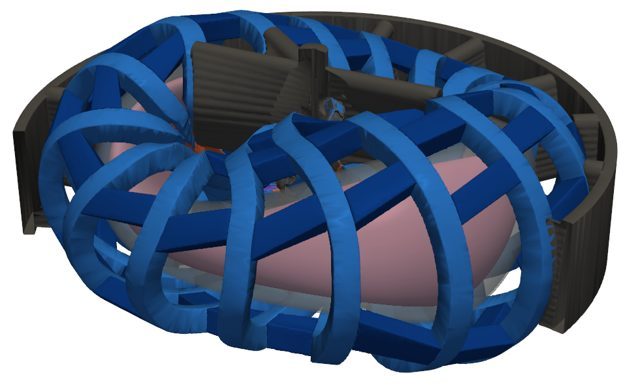
\includegraphics[width=\linewidth]{bilder/katalog/0048_en.jpg}\par\scriptsize \begin{tabular}{@{}l@{\,}r@{\quad}l@{\,}r@{}}coils & 16 & $\sigma_{99}$ & \num{2081} MPa \\conn./pair & 7 & max. & \num{19844} MPa \\$E_V$ & \num{160} GPa & strain & \num{1.39} \% \\distance & \num{0.29} & $B\cdot n$ & \num{10.18} ‰ \\steel & \num{13} kt & clear. & \num{2.32} m \\\end{tabular}\par violated: σ99 steel 1.4429, winding-pack strain, field error B·n. PicoGK: no overlap.\end{minipage}\par\vspace{6pt}
\clearpage
\begin{minipage}[t]{0.47\linewidth}\textbf{0049} \hfill \num{-462}\,\%\par \par\scriptsize \begin{tabular}{@{}l@{\,}r@{\quad}l@{\,}r@{}}coils & 16 & $\sigma_{99}$ & \num{2808} MPa \\conn./pair & 9 & max. & \num{9212} MPa \\$E_V$ & \num{84} GPa & strain & \num{1.07} \% \\distance & \num{0.21} & $B\cdot n$ & \num{2.42} ‰ \\steel & \num{18} kt & clear. & \num{1.74} m \\\end{tabular}\par violated: σ99 steel 1.4429, winding-pack strain.\end{minipage}\hfill
\begin{minipage}[t]{0.47\linewidth}\textbf{0051} \hfill \num{-130}\,\%\par \par\scriptsize \begin{tabular}{@{}l@{\,}r@{\quad}l@{\,}r@{}}coils & 20 & $\sigma_{99}$ & \num{1152} MPa \\conn./pair & 10 & max. & \num{2169} MPa \\$E_V$ & \num{37} GPa & strain & \num{0.50} \% \\distance & \num{0.17} & $B\cdot n$ & \num{3.32} ‰ \\steel & \num{15} kt & clear. & \num{1.50} m \\\end{tabular}\par violated: σ99 steel 1.4429, winding-pack strain, field error B·n.\end{minipage}\par\vspace{6pt}
\begin{minipage}[t]{0.47\linewidth}\textbf{0052} \hfill \num{-164}\,\%\par \par\scriptsize \begin{tabular}{@{}l@{\,}r@{\quad}l@{\,}r@{}}coils & 24 & $\sigma_{99}$ & \num{1321} MPa \\conn./pair & 13 & max. & \num{4323} MPa \\$E_V$ & \num{55} GPa & strain & \num{0.52} \% \\distance & \num{0.19} & $B\cdot n$ & \num{2.06} ‰ \\steel & \num{20} kt & clear. & \num{1.39} m \\\end{tabular}\par violated: σ99 steel 1.4429, winding-pack strain.\end{minipage}\hfill
\begin{minipage}[t]{0.47\linewidth}\textbf{0053} \hfill \num{-163}\,\%\par \par\scriptsize \begin{tabular}{@{}l@{\,}r@{\quad}l@{\,}r@{}}coils & 20 & $\sigma_{99}$ & \num{1314} MPa \\conn./pair & 6 & max. & \num{9639} MPa \\$E_V$ & \num{57} GPa & strain & \num{0.57} \% \\distance & \num{0.25} & $B\cdot n$ & \num{1.71} ‰ \\steel & \num{11} kt & clear. & \num{2.02} m \\\end{tabular}\par violated: σ99 steel 1.4429, winding-pack strain.\end{minipage}\par\vspace{6pt}
\clearpage
\begin{minipage}[t]{0.47\linewidth}\textbf{0054} \hfill \num{-138}\,\%\par \par\scriptsize \begin{tabular}{@{}l@{\,}r@{\quad}l@{\,}r@{}}coils & 16 & $\sigma_{99}$ & \num{963} MPa \\conn./pair & 7 & max. & \num{2479} MPa \\$E_V$ & \num{62} GPa & strain & \num{0.37} \% \\distance & \num{0.16} & $B\cdot n$ & \num{7.15} ‰ \\steel & \num{12} kt & clear. & \num{1.42} m \\\end{tabular}\par violated: σ99 steel 1.4429, winding-pack strain, field error B·n.\end{minipage}\hfill
\begin{minipage}[t]{0.47\linewidth}\textbf{0055}$^\ast$ \hfill \num{-192}\,\%\par \par\scriptsize \begin{tabular}{@{}l@{\,}r@{\quad}l@{\,}r@{}}coils & 20 & $\sigma_{99}$ & \num{413} MPa \\conn./pair & 14 & max. & \num{942} MPa \\$E_V$ & \num{38} GPa & strain & \num{0.18} \% \\distance & \num{0.13} & $B\cdot n$ & \num{2.84} ‰ \\steel & \num{32} kt & clear. & \num{1.15} m \\\end{tabular}\par violated: neutron fluence.\end{minipage}\par\vspace{6pt}
\begin{minipage}[t]{0.47\linewidth}\textbf{0056} \hfill \num{-423}\,\%\par \par\scriptsize \begin{tabular}{@{}l@{\,}r@{\quad}l@{\,}r@{}}coils & 20 & $\sigma_{99}$ & \num{2615} MPa \\conn./pair & 8 & max. & \num{13038} MPa \\$E_V$ & \num{59} GPa & strain & \num{1.21} \% \\distance & \num{0.28} & $B\cdot n$ & \num{2.25} ‰ \\steel & \num{16} kt & clear. & \num{2.06} m \\\end{tabular}\par violated: σ99 steel 1.4429, winding-pack strain.\end{minipage}\hfill
\begin{minipage}[t]{0.47\linewidth}\textbf{0057} \hfill \num{-111}\,\%\par \par\scriptsize \begin{tabular}{@{}l@{\,}r@{\quad}l@{\,}r@{}}coils & 20 & $\sigma_{99}$ & \num{1056} MPa \\conn./pair & 6 & max. & \num{4063} MPa \\$E_V$ & \num{31} GPa & strain & \num{0.39} \% \\distance & \num{0.24} & $B\cdot n$ & \num{2.18} ‰ \\steel & \num{14} kt & clear. & \num{1.60} m \\\end{tabular}\par violated: σ99 steel 1.4429, winding-pack strain.\end{minipage}\par\vspace{6pt}
\clearpage
\begin{minipage}[t]{0.47\linewidth}\textbf{0058} \hfill \num{-124}\,\%\par \par\scriptsize \begin{tabular}{@{}l@{\,}r@{\quad}l@{\,}r@{}}coils & 16 & $\sigma_{99}$ & \num{689} MPa \\conn./pair & 10 & max. & \num{2099} MPa \\$E_V$ & \num{32} GPa & strain & \num{0.29} \% \\distance & \num{0.23} & $B\cdot n$ & \num{6.71} ‰ \\steel & \num{29} kt & clear. & \num{1.60} m \\\end{tabular}\par violated: σ99 steel 1.4429, field error B·n.\end{minipage}\hfill
\begin{minipage}[t]{0.47\linewidth}\textbf{0059} \hfill \num{-132}\,\%\par \par\scriptsize \begin{tabular}{@{}l@{\,}r@{\quad}l@{\,}r@{}}coils & 16 & $\sigma_{99}$ & \num{1161} MPa \\conn./pair & 11 & max. & \num{4304} MPa \\$E_V$ & \num{110} GPa & strain & \num{0.57} \% \\distance & \num{0.19} & $B\cdot n$ & \num{2.27} ‰ \\steel & \num{31} kt & clear. & \num{1.48} m \\\end{tabular}\par violated: σ99 steel 1.4429, winding-pack strain.\end{minipage}\par\vspace{6pt}
\begin{minipage}[t]{0.47\linewidth}\textbf{0060}$^\ast$ \hfill \num{-41}\,\%\par \par\scriptsize \begin{tabular}{@{}l@{\,}r@{\quad}l@{\,}r@{}}coils & 24 & $\sigma_{99}$ & \num{704} MPa \\conn./pair & 13 & max. & \num{1499} MPa \\$E_V$ & \num{155} GPa & strain & \num{0.29} \% \\distance & \num{0.22} & $B\cdot n$ & \num{1.61} ‰ \\steel & \num{16} kt & clear. & \num{1.66} m \\\end{tabular}\par violated: σ99 steel 1.4429.\end{minipage}\hfill
\begin{minipage}[t]{0.47\linewidth}\textbf{0061} \hfill \num{30}\,\%\par \par\scriptsize \begin{tabular}{@{}l@{\,}r@{\quad}l@{\,}r@{}}coils & 24 & $\sigma_{99}$ & \num{351} MPa \\conn./pair & 10 & max. & \num{725} MPa \\$E_V$ & \num{93} GPa & strain & \num{0.17} \% \\distance & \num{0.20} & $B\cdot n$ & \num{1.49} ‰ \\steel & \num{19} kt & clear. & \num{1.62} m \\\end{tabular}\par \textbf{admissible}.\end{minipage}\par\vspace{6pt}
\clearpage
\begin{minipage}[t]{0.47\linewidth}\textbf{0062} \hfill \num{-427}\,\%\par \par\scriptsize \begin{tabular}{@{}l@{\,}r@{\quad}l@{\,}r@{}}coils & 24 & $\sigma_{99}$ & \num{2627} MPa \\conn./pair & 9 & max. & \num{13807} MPa \\$E_V$ & \num{21} GPa & strain & \num{1.58} \% \\distance & \num{0.30} & $B\cdot n$ & \num{3.27} ‰ \\steel & \num{17} kt & clear. & \num{2.40} m \\\end{tabular}\par violated: σ99 steel 1.4429, winding-pack strain, field error B·n.\end{minipage}\hfill
\begin{minipage}[t]{0.47\linewidth}\textbf{0063}$^\ast$ \hfill \num{-24}\,\%\par \par\scriptsize \begin{tabular}{@{}l@{\,}r@{\quad}l@{\,}r@{}}coils & 20 & $\sigma_{99}$ & \num{595} MPa \\conn./pair & 14 & max. & \num{4265} MPa \\$E_V$ & \num{43} GPa & strain & \num{0.37} \% \\distance & \num{0.18} & $B\cdot n$ & \num{0.75} ‰ \\steel & \num{41} kt & clear. & \num{1.53} m \\\end{tabular}\par violated: σ99 steel 1.4429, winding-pack strain.\end{minipage}\par\vspace{6pt}
\begin{minipage}[t]{0.47\linewidth}\textbf{0064} \hfill \num{-90}\,\%\par \par\scriptsize \begin{tabular}{@{}l@{\,}r@{\quad}l@{\,}r@{}}coils & 16 & $\sigma_{99}$ & \num{683} MPa \\conn./pair & 12 & max. & \num{5601} MPa \\$E_V$ & \num{131} GPa & strain & \num{0.35} \% \\distance & \num{0.27} & $B\cdot n$ & \num{5.70} ‰ \\steel & \num{22} kt & clear. & \num{1.85} m \\\end{tabular}\par violated: σ99 steel 1.4429, winding-pack strain, field error B·n.\end{minipage}\hfill
\begin{minipage}[t]{0.47\linewidth}\textbf{0065} \hfill \num{-32}\,\%\par \par\scriptsize \begin{tabular}{@{}l@{\,}r@{\quad}l@{\,}r@{}}coils & 20 & $\sigma_{99}$ & \num{660} MPa \\conn./pair & 9 & max. & \num{1210} MPa \\$E_V$ & \num{48} GPa & strain & \num{0.31} \% \\distance & \num{0.17} & $B\cdot n$ & \num{1.97} ‰ \\steel & \num{15} kt & clear. & \num{1.61} m \\\end{tabular}\par violated: σ99 steel 1.4429, winding-pack strain.\end{minipage}\par\vspace{6pt}
\clearpage
\begin{minipage}[t]{0.47\linewidth}\textbf{0067} \hfill \num{-100}\,\%\par \par\scriptsize \begin{tabular}{@{}l@{\,}r@{\quad}l@{\,}r@{}}coils & 20 & $\sigma_{99}$ & \num{999} MPa \\conn./pair & 11 & max. & \num{2826} MPa \\$E_V$ & \num{82} GPa & strain & \num{0.47} \% \\distance & \num{0.20} & $B\cdot n$ & \num{3.08} ‰ \\steel & \num{28} kt & clear. & \num{1.53} m \\\end{tabular}\par violated: σ99 steel 1.4429, winding-pack strain, field error B·n.\end{minipage}\hfill
\begin{minipage}[t]{0.47\linewidth}\textbf{0068} \hfill \num{-102}\,\%\par \par\scriptsize \begin{tabular}{@{}l@{\,}r@{\quad}l@{\,}r@{}}coils & 20 & $\sigma_{99}$ & \num{1012} MPa \\conn./pair & 10 & max. & \num{2393} MPa \\$E_V$ & \num{75} GPa & strain & \num{0.42} \% \\distance & \num{0.12} & $B\cdot n$ & \num{1.57} ‰ \\steel & \num{18} kt & clear. & \num{1.53} m \\\end{tabular}\par violated: σ99 steel 1.4429, winding-pack strain.\end{minipage}\par\vspace{6pt}
\begin{minipage}[t]{0.47\linewidth}\textbf{0069} \hfill \num{-225}\,\%\par \par\scriptsize \begin{tabular}{@{}l@{\,}r@{\quad}l@{\,}r@{}}coils & 20 & $\sigma_{99}$ & \num{1624} MPa \\conn./pair & 7 & max. & \num{16704} MPa \\$E_V$ & \num{130} GPa & strain & \num{0.84} \% \\distance & \num{0.29} & $B\cdot n$ & \num{6.85} ‰ \\steel & \num{15} kt & clear. & \num{2.16} m \\\end{tabular}\par violated: σ99 steel 1.4429, winding-pack strain, field error B·n.\end{minipage}\hfill
\begin{minipage}[t]{0.47\linewidth}\textbf{0070} \hfill \num{-134}\,\%\par \par\scriptsize \begin{tabular}{@{}l@{\,}r@{\quad}l@{\,}r@{}}coils & 24 & $\sigma_{99}$ & \num{1172} MPa \\conn./pair & 14 & max. & \num{6574} MPa \\$E_V$ & \num{119} GPa & strain & \num{0.56} \% \\distance & \num{0.18} & $B\cdot n$ & \num{0.83} ‰ \\steel & \num{28} kt & clear. & \num{1.51} m \\\end{tabular}\par violated: σ99 steel 1.4429, winding-pack strain.\end{minipage}\par\vspace{6pt}
\clearpage
\begin{minipage}[t]{0.47\linewidth}\textbf{0071} \hfill \num{-121}\,\%\par \par\scriptsize \begin{tabular}{@{}l@{\,}r@{\quad}l@{\,}r@{}}coils & 24 & $\sigma_{99}$ & \num{1075} MPa \\conn./pair & 12 & max. & \num{5955} MPa \\$E_V$ & \num{192} GPa & strain & \num{0.66} \% \\distance & \num{0.25} & $B\cdot n$ & \num{1.55} ‰ \\steel & \num{30} kt & clear. & \num{1.61} m \\\end{tabular}\par violated: σ99 steel 1.4429, winding-pack strain.\end{minipage}\hfill
\begin{minipage}[t]{0.47\linewidth}\textbf{0072} \hfill \num{-119}\,\%\par \par\scriptsize \begin{tabular}{@{}l@{\,}r@{\quad}l@{\,}r@{}}coils & 24 & $\sigma_{99}$ & \num{1093} MPa \\conn./pair & 9 & max. & \num{8828} MPa \\$E_V$ & \num{95} GPa & strain & \num{0.56} \% \\distance & \num{0.17} & $B\cdot n$ & \num{2.35} ‰ \\steel & \num{22} kt & clear. & \num{1.33} m \\\end{tabular}\par violated: σ99 steel 1.4429, winding-pack strain.\end{minipage}\par\vspace{6pt}
\begin{minipage}[t]{0.47\linewidth}\textbf{0073} \hfill \num{-363}\,\%\par \par\scriptsize \begin{tabular}{@{}l@{\,}r@{\quad}l@{\,}r@{}}coils & 16 & $\sigma_{99}$ & \num{1030} MPa \\conn./pair & 12 & max. & \num{50101} MPa \\$E_V$ & \num{52} GPa & strain & \num{0.71} \% \\distance & \num{0.24} & $B\cdot n$ & \num{13.89} ‰ \\steel & \num{23} kt & clear. & \num{1.54} m \\\end{tabular}\par violated: σ99 steel 1.4429, winding-pack strain, field error B·n.\end{minipage}\hfill
\begin{minipage}[t]{0.47\linewidth}\textbf{0074} \hfill \num{-243}\,\%\par \par\scriptsize \begin{tabular}{@{}l@{\,}r@{\quad}l@{\,}r@{}}coils & 16 & $\sigma_{99}$ & \num{1715} MPa \\conn./pair & 6 & max. & \num{23336} MPa \\$E_V$ & \num{85} GPa & strain & \num{0.65} \% \\distance & \num{0.26} & $B\cdot n$ & \num{2.71} ‰ \\steel & \num{14} kt & clear. & \num{1.74} m \\\end{tabular}\par violated: σ99 steel 1.4429, winding-pack strain.\end{minipage}\par\vspace{6pt}
\clearpage
\begin{minipage}[t]{0.47\linewidth}\textbf{0075} \hfill \num{-54}\,\%\par \par\scriptsize \begin{tabular}{@{}l@{\,}r@{\quad}l@{\,}r@{}}coils & 20 & $\sigma_{99}$ & \num{477} MPa \\conn./pair & 10 & max. & \num{1064} MPa \\$E_V$ & \num{163} GPa & strain & \num{0.20} \% \\distance & \num{0.20} & $B\cdot n$ & \num{4.62} ‰ \\steel & \num{18} kt & clear. & \num{1.25} m \\\end{tabular}\par violated: neutron fluence, field error B·n.\end{minipage}\hfill
\begin{minipage}[t]{0.47\linewidth}\textbf{0076} \hfill \num{-350}\,\%\par \par\scriptsize \begin{tabular}{@{}l@{\,}r@{\quad}l@{\,}r@{}}coils & 20 & $\sigma_{99}$ & \num{1983} MPa \\conn./pair & 9 & max. & \num{10425} MPa \\$E_V$ & \num{33} GPa & strain & \num{1.35} \% \\distance & \num{0.27} & $B\cdot n$ & \num{2.07} ‰ \\steel & \num{23} kt & clear. & \num{2.13} m \\\end{tabular}\par violated: σ99 steel 1.4429, winding-pack strain.\end{minipage}\par\vspace{6pt}
\begin{minipage}[t]{0.47\linewidth}\textbf{0077} \hfill \num{-56}\,\%\par \par\scriptsize \begin{tabular}{@{}l@{\,}r@{\quad}l@{\,}r@{}}coils & 24 & $\sigma_{99}$ & \num{779} MPa \\conn./pair & 10 & max. & \num{1288} MPa \\$E_V$ & \num{47} GPa & strain & \num{0.31} \% \\distance & \num{0.21} & $B\cdot n$ & \num{1.07} ‰ \\steel & \num{14} kt & clear. & \num{1.65} m \\\end{tabular}\par violated: σ99 steel 1.4429, winding-pack strain.\end{minipage}\hfill
\begin{minipage}[t]{0.47\linewidth}\textbf{0078} \hfill \num{-284}\,\%\par \par\scriptsize \begin{tabular}{@{}l@{\,}r@{\quad}l@{\,}r@{}}coils & 24 & $\sigma_{99}$ & \num{1919} MPa \\conn./pair & 8 & max. & \num{14222} MPa \\$E_V$ & \num{36} GPa & strain & \num{0.85} \% \\distance & \num{0.24} & $B\cdot n$ & \num{1.52} ‰ \\steel & \num{18} kt & clear. & \num{1.85} m \\\end{tabular}\par violated: σ99 steel 1.4429, winding-pack strain.\end{minipage}\par\vspace{6pt}
\clearpage
\begin{minipage}[t]{0.47\linewidth}\textbf{0079} \hfill \num{-164}\,\%\par \par\scriptsize \begin{tabular}{@{}l@{\,}r@{\quad}l@{\,}r@{}}coils & 20 & $\sigma_{99}$ & \num{1320} MPa \\conn./pair & 13 & max. & \num{8604} MPa \\$E_V$ & \num{30} GPa & strain & \num{0.66} \% \\distance & \num{0.27} & $B\cdot n$ & \num{1.17} ‰ \\steel & \num{23} kt & clear. & \num{2.00} m \\\end{tabular}\par violated: σ99 steel 1.4429, winding-pack strain.\end{minipage}\hfill
\begin{minipage}[t]{0.47\linewidth}\textbf{0080} \hfill \num{-61}\,\%\par \par\scriptsize \begin{tabular}{@{}l@{\,}r@{\quad}l@{\,}r@{}}coils & 16 & $\sigma_{99}$ & \num{803} MPa \\conn./pair & 12 & max. & \num{1759} MPa \\$E_V$ & \num{65} GPa & strain & \num{0.32} \% \\distance & \num{0.13} & $B\cdot n$ & \num{3.98} ‰ \\steel & \num{21} kt & clear. & \num{1.47} m \\\end{tabular}\par violated: σ99 steel 1.4429, winding-pack strain, field error B·n.\end{minipage}\par\vspace{6pt}
\begin{minipage}[t]{0.47\linewidth}\textbf{0081} \hfill \num{-36}\,\%\par \par\scriptsize \begin{tabular}{@{}l@{\,}r@{\quad}l@{\,}r@{}}coils & 24 & $\sigma_{99}$ & \num{577} MPa \\conn./pair & 9 & max. & \num{5361} MPa \\$E_V$ & \num{97} GPa & strain & \num{0.41} \% \\distance & \num{0.27} & $B\cdot n$ & \num{2.32} ‰ \\steel & \num{19} kt & clear. & \num{2.17} m \\\end{tabular}\par violated: σ99 steel 1.4429, winding-pack strain.\end{minipage}\hfill
\begin{minipage}[t]{0.47\linewidth}\textbf{0082} \hfill \num{-418}\,\%\par \par\scriptsize \begin{tabular}{@{}l@{\,}r@{\quad}l@{\,}r@{}}coils & 20 & $\sigma_{99}$ & \num{2591} MPa \\conn./pair & 8 & max. & \num{34831} MPa \\$E_V$ & \num{23} GPa & strain & \num{1.50} \% \\distance & \num{0.16} & $B\cdot n$ & \num{1.75} ‰ \\steel & \num{17} kt & clear. & \num{1.72} m \\\end{tabular}\par violated: σ99 steel 1.4429, winding-pack strain.\end{minipage}\par\vspace{6pt}
\clearpage
\begin{minipage}[t]{0.47\linewidth}\textbf{0083} \hfill \num{-99}\,\%\par \par\scriptsize \begin{tabular}{@{}l@{\,}r@{\quad}l@{\,}r@{}}coils & 16 & $\sigma_{99}$ & \num{996} MPa \\conn./pair & 6 & max. & \num{5784} MPa \\$E_V$ & \num{27} GPa & strain & \num{0.54} \% \\distance & \num{0.26} & $B\cdot n$ & \num{5.30} ‰ \\steel & \num{14} kt & clear. & \num{2.05} m \\\end{tabular}\par violated: σ99 steel 1.4429, winding-pack strain, field error B·n.\end{minipage}\hfill
\begin{minipage}[t]{0.47\linewidth}\textbf{0084}$^\ast$ \hfill \num{-225}\,\%\par \par\scriptsize \begin{tabular}{@{}l@{\,}r@{\quad}l@{\,}r@{}}coils & 16 & $\sigma_{99}$ & \num{462} MPa \\conn./pair & 14 & max. & \num{1018} MPa \\$E_V$ & \num{63} GPa & strain & \num{0.20} \% \\distance & \num{0.19} & $B\cdot n$ & \num{9.75} ‰ \\steel & \num{20} kt & clear. & \num{1.26} m \\\end{tabular}\par violated: neutron fluence, field error B·n.\end{minipage}\par\vspace{6pt}
\begin{minipage}[t]{0.47\linewidth}\textbf{0085} \hfill \num{-31}\,\%\par \par\scriptsize \begin{tabular}{@{}l@{\,}r@{\quad}l@{\,}r@{}}coils & 20 & $\sigma_{99}$ & \num{608} MPa \\conn./pair & 10 & max. & \num{2067} MPa \\$E_V$ & \num{22} GPa & strain & \num{0.28} \% \\distance & \num{0.19} & $B\cdot n$ & \num{2.00} ‰ \\steel & \num{30} kt & clear. & \num{1.23} m \\\end{tabular}\par violated: σ99 steel 1.4429, neutron fluence.\end{minipage}\hfill
\begin{minipage}[t]{0.47\linewidth}\textbf{0086} \hfill \num{-168}\,\%\par \par\scriptsize \begin{tabular}{@{}l@{\,}r@{\quad}l@{\,}r@{}}coils & 16 & $\sigma_{99}$ & \num{1339} MPa \\conn./pair & 13 & max. & \num{5294} MPa \\$E_V$ & \num{67} GPa & strain & \num{0.53} \% \\distance & \num{0.20} & $B\cdot n$ & \num{2.87} ‰ \\steel & \num{21} kt & clear. & \num{1.64} m \\\end{tabular}\par violated: σ99 steel 1.4429, winding-pack strain.\end{minipage}\par\vspace{6pt}
\clearpage
\begin{minipage}[t]{0.47\linewidth}\textbf{0087} \hfill \num{-267}\,\%\par \par\scriptsize \begin{tabular}{@{}l@{\,}r@{\quad}l@{\,}r@{}}coils & 20 & $\sigma_{99}$ & \num{1837} MPa \\conn./pair & 6 & max. & \num{11946} MPa \\$E_V$ & \num{30} GPa & strain & \num{0.94} \% \\distance & \num{0.21} & $B\cdot n$ & \num{1.40} ‰ \\steel & \num{17} kt & clear. & \num{1.32} m \\\end{tabular}\par violated: σ99 steel 1.4429, winding-pack strain.\end{minipage}\hfill
\begin{minipage}[t]{0.47\linewidth}\textbf{0088} \hfill \num{-3286}\,\%\par \par\scriptsize \begin{tabular}{@{}l@{\,}r@{\quad}l@{\,}r@{}}coils & 24 & $\sigma_{99}$ & \num{1478} MPa \\conn./pair & 13 & max. & \num{5859} MPa \\$E_V$ & \num{86} GPa & strain & \num{0.71} \% \\distance & \num{0.14} & $B\cdot n$ & \num{1.92} ‰ \\steel & \num{33} kt & clear. & \num{0.91} m \\\end{tabular}\par violated: σ99 steel 1.4429, winding-pack strain, package space, nuclear heating, neutron fluence.\end{minipage}\par\vspace{6pt}
\begin{minipage}[t]{0.47\linewidth}\textbf{0089} \hfill \num{-546}\,\%\par \par\scriptsize \begin{tabular}{@{}l@{\,}r@{\quad}l@{\,}r@{}}coils & 24 & $\sigma_{99}$ & \num{645} MPa \\conn./pair & 12 & max. & \num{2827} MPa \\$E_V$ & \num{22} GPa & strain & \num{0.30} \% \\distance & \num{0.15} & $B\cdot n$ & \num{2.16} ‰ \\steel & \num{30} kt & clear. & \num{1.07} m \\\end{tabular}\par violated: σ99 steel 1.4429, package space, nuclear heating, neutron fluence.\end{minipage}\hfill
\begin{minipage}[t]{0.47\linewidth}\textbf{0090} \hfill \num{-286}\,\%\par \par\scriptsize \begin{tabular}{@{}l@{\,}r@{\quad}l@{\,}r@{}}coils & 20 & $\sigma_{99}$ & \num{1929} MPa \\conn./pair & 6 & max. & \num{10870} MPa \\$E_V$ & \num{161} GPa & strain & \num{0.91} \% \\distance & \num{0.19} & $B\cdot n$ & \num{2.84} ‰ \\steel & \num{17} kt & clear. & \num{1.36} m \\\end{tabular}\par violated: σ99 steel 1.4429, winding-pack strain.\end{minipage}\par\vspace{6pt}
\clearpage
\begin{minipage}[t]{0.47\linewidth}\textbf{0091} \hfill \num{-70}\,\%\par \par\scriptsize \begin{tabular}{@{}l@{\,}r@{\quad}l@{\,}r@{}}coils & 16 & $\sigma_{99}$ & \num{848} MPa \\conn./pair & 10 & max. & \num{2510} MPa \\$E_V$ & \num{42} GPa & strain & \num{0.38} \% \\distance & \num{0.22} & $B\cdot n$ & \num{4.47} ‰ \\steel & \num{23} kt & clear. & \num{1.52} m \\\end{tabular}\par violated: σ99 steel 1.4429, winding-pack strain, field error B·n.\end{minipage}\hfill
\begin{minipage}[t]{0.47\linewidth}\textbf{0092} \hfill \num{-151}\,\%\par \par\scriptsize \begin{tabular}{@{}l@{\,}r@{\quad}l@{\,}r@{}}coils & 20 & $\sigma_{99}$ & \num{1195} MPa \\conn./pair & 10 & max. & \num{14134} MPa \\$E_V$ & \num{44} GPa & strain & \num{0.75} \% \\distance & \num{0.23} & $B\cdot n$ & \num{3.37} ‰ \\steel & \num{23} kt & clear. & \num{1.43} m \\\end{tabular}\par violated: σ99 steel 1.4429, winding-pack strain, field error B·n.\end{minipage}\par\vspace{6pt}
\begin{minipage}[t]{0.47\linewidth}\textbf{0093} \hfill \num{27}\,\%\par \par\scriptsize \begin{tabular}{@{}l@{\,}r@{\quad}l@{\,}r@{}}coils & 24 & $\sigma_{99}$ & \num{283} MPa \\conn./pair & 8 & max. & \num{1190} MPa \\$E_V$ & \num{64} GPa & strain & \num{0.16} \% \\distance & \num{0.21} & $B\cdot n$ & \num{1.45} ‰ \\steel & \num{28} kt & clear. & \num{1.37} m \\\end{tabular}\par \textbf{admissible}.\end{minipage}\hfill
\begin{minipage}[t]{0.47\linewidth}\textbf{0095} \hfill \num{-55}\,\%\par \par\scriptsize \begin{tabular}{@{}l@{\,}r@{\quad}l@{\,}r@{}}coils & 16 & $\sigma_{99}$ & \num{773} MPa \\conn./pair & 8 & max. & \num{2138} MPa \\$E_V$ & \num{186} GPa & strain & \num{0.32} \% \\distance & \num{0.19} & $B\cdot n$ & \num{3.25} ‰ \\steel & \num{22} kt & clear. & \num{1.28} m \\\end{tabular}\par violated: σ99 steel 1.4429, winding-pack strain, field error B·n.\end{minipage}\par\vspace{6pt}
\clearpage
\begin{minipage}[t]{0.47\linewidth}\textbf{0096} \hfill \num{-185}\,\%\par \par\scriptsize \begin{tabular}{@{}l@{\,}r@{\quad}l@{\,}r@{}}coils & 16 & $\sigma_{99}$ & \num{1006} MPa \\conn./pair & 11 & max. & \num{3209} MPa \\$E_V$ & \num{25} GPa & strain & \num{0.40} \% \\distance & \num{0.25} & $B\cdot n$ & \num{8.54} ‰ \\steel & \num{15} kt & clear. & \num{1.85} m \\\end{tabular}\par violated: σ99 steel 1.4429, winding-pack strain, field error B·n.\end{minipage}\hfill
\begin{minipage}[t]{0.47\linewidth}\textbf{0097} \hfill \num{-331}\,\%\par \par\scriptsize \begin{tabular}{@{}l@{\,}r@{\quad}l@{\,}r@{}}coils & 24 & $\sigma_{99}$ & \num{2155} MPa \\conn./pair & 7 & max. & \num{28026} MPa \\$E_V$ & \num{99} GPa & strain & \num{0.95} \% \\distance & \num{0.14} & $B\cdot n$ & \num{2.76} ‰ \\steel & \num{14} kt & clear. & \num{1.30} m \\\end{tabular}\par violated: σ99 steel 1.4429, winding-pack strain.\end{minipage}\par\vspace{6pt}
\begin{minipage}[t]{0.47\linewidth}\textbf{0098} \hfill \num{-350}\,\%\par \par\scriptsize \begin{tabular}{@{}l@{\,}r@{\quad}l@{\,}r@{}}coils & 20 & $\sigma_{99}$ & \num{2250} MPa \\conn./pair & 13 & max. & \num{13304} MPa \\$E_V$ & \num{25} GPa & strain & \num{1.30} \% \\distance & \num{0.29} & $B\cdot n$ & \num{6.96} ‰ \\steel & \num{20} kt & clear. & \num{2.18} m \\\end{tabular}\par violated: σ99 steel 1.4429, winding-pack strain, field error B·n.\end{minipage}\hfill
\begin{minipage}[t]{0.47\linewidth}\textbf{0099} \hfill \num{-305}\,\%\par \par\scriptsize \begin{tabular}{@{}l@{\,}r@{\quad}l@{\,}r@{}}coils & 20 & $\sigma_{99}$ & \num{2025} MPa \\conn./pair & 8 & max. & \num{7095} MPa \\$E_V$ & \num{62} GPa & strain & \num{0.97} \% \\distance & \num{0.28} & $B\cdot n$ & \num{2.32} ‰ \\steel & \num{20} kt & clear. & \num{1.89} m \\\end{tabular}\par violated: σ99 steel 1.4429, winding-pack strain.\end{minipage}\par\vspace{6pt}
\clearpage
\begin{minipage}[t]{0.47\linewidth}\textbf{0100} \hfill \num{-103}\,\%\par \par\scriptsize \begin{tabular}{@{}l@{\,}r@{\quad}l@{\,}r@{}}coils & 24 & $\sigma_{99}$ & \num{441} MPa \\conn./pair & 7 & max. & \num{788} MPa \\$E_V$ & \num{59} GPa & strain & \num{0.20} \% \\distance & \num{0.13} & $B\cdot n$ & \num{2.37} ‰ \\steel & \num{19} kt & clear. & \num{1.19} m \\\end{tabular}\par violated: neutron fluence.\end{minipage}\hfill
\begin{minipage}[t]{0.47\linewidth}\textbf{0101} \hfill \num{-36}\,\%\par \par\scriptsize \begin{tabular}{@{}l@{\,}r@{\quad}l@{\,}r@{}}coils & 20 & $\sigma_{99}$ & \num{681} MPa \\conn./pair & 6 & max. & \num{1564} MPa \\$E_V$ & \num{68} GPa & strain & \num{0.31} \% \\distance & \num{0.13} & $B\cdot n$ & \num{2.20} ‰ \\steel & \num{16} kt & clear. & \num{1.51} m \\\end{tabular}\par violated: σ99 steel 1.4429, winding-pack strain.\end{minipage}\par\vspace{6pt}
\begin{minipage}[t]{0.47\linewidth}\textbf{0102} \hfill \num{-254}\,\%\par \par\scriptsize \begin{tabular}{@{}l@{\,}r@{\quad}l@{\,}r@{}}coils & 16 & $\sigma_{99}$ & \num{1358} MPa \\conn./pair & 11 & max. & \num{12788} MPa \\$E_V$ & \num{98} GPa & strain & \num{0.94} \% \\distance & \num{0.25} & $B\cdot n$ & \num{10.62} ‰ \\steel & \num{21} kt & clear. & \num{1.79} m \\\end{tabular}\par violated: σ99 steel 1.4429, winding-pack strain, field error B·n.\end{minipage}\hfill
\begin{minipage}[t]{0.47\linewidth}\textbf{0103} \hfill \num{-8}\,\%\par \par\scriptsize \begin{tabular}{@{}l@{\,}r@{\quad}l@{\,}r@{}}coils & 20 & $\sigma_{99}$ & \num{440} MPa \\conn./pair & 11 & max. & \num{738} MPa \\$E_V$ & \num{38} GPa & strain & \num{0.19} \% \\distance & \num{0.18} & $B\cdot n$ & \num{2.66} ‰ \\steel & \num{21} kt & clear. & \num{1.25} m \\\end{tabular}\par violated: neutron fluence.\end{minipage}\par\vspace{6pt}
\clearpage
\begin{minipage}[t]{0.47\linewidth}\textbf{0104} \hfill \num{-178}\,\%\par \par\scriptsize \begin{tabular}{@{}l@{\,}r@{\quad}l@{\,}r@{}}coils & 16 & $\sigma_{99}$ & \num{1389} MPa \\conn./pair & 11 & max. & \num{6056} MPa \\$E_V$ & \num{43} GPa & strain & \num{0.70} \% \\distance & \num{0.26} & $B\cdot n$ & \num{2.22} ‰ \\steel & \num{21} kt & clear. & \num{1.99} m \\\end{tabular}\par violated: σ99 steel 1.4429, winding-pack strain.\end{minipage}\hfill
\begin{minipage}[t]{0.47\linewidth}\textbf{0105} \hfill \num{-102}\,\%\par \par\scriptsize \begin{tabular}{@{}l@{\,}r@{\quad}l@{\,}r@{}}coils & 24 & $\sigma_{99}$ & \num{1012} MPa \\conn./pair & 14 & max. & \num{5267} MPa \\$E_V$ & \num{39} GPa & strain & \num{0.57} \% \\distance & \num{0.19} & $B\cdot n$ & \num{1.18} ‰ \\steel & \num{28} kt & clear. & \num{1.41} m \\\end{tabular}\par violated: σ99 steel 1.4429, winding-pack strain.\end{minipage}\par\vspace{6pt}
\begin{minipage}[t]{0.47\linewidth}\textbf{0106} \hfill \num{-214}\,\%\par \par\scriptsize \begin{tabular}{@{}l@{\,}r@{\quad}l@{\,}r@{}}coils & 24 & $\sigma_{99}$ & \num{1568} MPa \\conn./pair & 6 & max. & \num{11316} MPa \\$E_V$ & \num{94} GPa & strain & \num{0.94} \% \\distance & \num{0.27} & $B\cdot n$ & \num{0.92} ‰ \\steel & \num{18} kt & clear. & \num{2.02} m \\\end{tabular}\par violated: σ99 steel 1.4429, winding-pack strain.\end{minipage}\hfill
\begin{minipage}[t]{0.47\linewidth}\textbf{0107} \hfill \num{-93}\,\%\par \par\scriptsize \begin{tabular}{@{}l@{\,}r@{\quad}l@{\,}r@{}}coils & 16 & $\sigma_{99}$ & \num{469} MPa \\conn./pair & 10 & max. & \num{1255} MPa \\$E_V$ & \num{124} GPa & strain & \num{0.22} \% \\distance & \num{0.15} & $B\cdot n$ & \num{5.79} ‰ \\steel & \num{25} kt & clear. & \num{1.39} m \\\end{tabular}\par violated: field error B·n.\end{minipage}\par\vspace{6pt}
\clearpage
\begin{minipage}[t]{0.47\linewidth}\textbf{0110} \hfill \num{-220}\,\%\par \par\scriptsize \begin{tabular}{@{}l@{\,}r@{\quad}l@{\,}r@{}}coils & 16 & $\sigma_{99}$ & \num{1601} MPa \\conn./pair & 12 & max. & \num{12212} MPa \\$E_V$ & \num{27} GPa & strain & \num{0.73} \% \\distance & \num{0.23} & $B\cdot n$ & \num{2.82} ‰ \\steel & \num{27} kt & clear. & \num{1.61} m \\\end{tabular}\par violated: σ99 steel 1.4429, winding-pack strain.\end{minipage}\hfill
\begin{minipage}[t]{0.47\linewidth}\textbf{0111} \hfill \num{-225}\,\%\par \par\scriptsize \begin{tabular}{@{}l@{\,}r@{\quad}l@{\,}r@{}}coils & 16 & $\sigma_{99}$ & \num{1627} MPa \\conn./pair & 11 & max. & \num{10386} MPa \\$E_V$ & \num{86} GPa & strain & \num{0.90} \% \\distance & \num{0.30} & $B\cdot n$ & \num{8.08} ‰ \\steel & \num{20} kt & clear. & \num{2.12} m \\\end{tabular}\par violated: σ99 steel 1.4429, winding-pack strain, field error B·n.\end{minipage}\par\vspace{6pt}
\begin{minipage}[t]{0.47\linewidth}\textbf{0112} \hfill \num{-80}\,\%\par \par\scriptsize \begin{tabular}{@{}l@{\,}r@{\quad}l@{\,}r@{}}coils & 16 & $\sigma_{99}$ & \num{902} MPa \\conn./pair & 11 & max. & \num{2045} MPa \\$E_V$ & \num{54} GPa & strain & \num{0.35} \% \\distance & \num{0.15} & $B\cdot n$ & \num{3.81} ‰ \\steel & \num{18} kt & clear. & \num{1.56} m \\\end{tabular}\par violated: σ99 steel 1.4429, winding-pack strain, field error B·n.\end{minipage}\hfill
\begin{minipage}[t]{0.47\linewidth}\textbf{0113} \hfill \num{-203}\,\%\par \par\scriptsize \begin{tabular}{@{}l@{\,}r@{\quad}l@{\,}r@{}}coils & 16 & $\sigma_{99}$ & \num{535} MPa \\conn./pair & 14 & max. & \num{1625} MPa \\$E_V$ & \num{47} GPa & strain & \num{0.22} \% \\distance & \num{0.14} & $B\cdot n$ & \num{9.10} ‰ \\steel & \num{24} kt & clear. & \num{1.22} m \\\end{tabular}\par violated: σ99 steel 1.4429, neutron fluence, field error B·n.\end{minipage}\par\vspace{6pt}
\clearpage
\begin{minipage}[t]{0.47\linewidth}\textbf{0114} \hfill \num{-200}\,\%\par \par\scriptsize \begin{tabular}{@{}l@{\,}r@{\quad}l@{\,}r@{}}coils & 20 & $\sigma_{99}$ & \num{1501} MPa \\conn./pair & 7 & max. & \num{14380} MPa \\$E_V$ & \num{90} GPa & strain & \num{0.78} \% \\distance & \num{0.22} & $B\cdot n$ & \num{2.18} ‰ \\steel & \num{19} kt & clear. & \num{1.60} m \\\end{tabular}\par violated: σ99 steel 1.4429, winding-pack strain.\end{minipage}\hfill
\begin{minipage}[t]{0.47\linewidth}\textbf{0115} \hfill \num{-76}\,\%\par \par\scriptsize \begin{tabular}{@{}l@{\,}r@{\quad}l@{\,}r@{}}coils & 24 & $\sigma_{99}$ & \num{698} MPa \\conn./pair & 6 & max. & \num{2102} MPa \\$E_V$ & \num{41} GPa & strain & \num{0.34} \% \\distance & \num{0.21} & $B\cdot n$ & \num{1.62} ‰ \\steel & \num{15} kt & clear. & \num{1.20} m \\\end{tabular}\par violated: σ99 steel 1.4429, winding-pack strain, neutron fluence.\end{minipage}\par\vspace{6pt}
\begin{minipage}[t]{0.47\linewidth}\textbf{0116} \hfill \num{-1627}\,\%\par \par\scriptsize \begin{tabular}{@{}l@{\,}r@{\quad}l@{\,}r@{}}coils & 24 & $\sigma_{99}$ & \num{1129} MPa \\conn./pair & 7 & max. & \num{7726} MPa \\$E_V$ & \num{33} GPa & strain & \num{0.63} \% \\distance & \num{0.14} & $B\cdot n$ & \num{1.60} ‰ \\steel & \num{26} kt & clear. & \num{0.98} m \\\end{tabular}\par violated: σ99 steel 1.4429, winding-pack strain, package space, nuclear heating, neutron fluence.\end{minipage}\hfill
\begin{minipage}[t]{0.47\linewidth}\textbf{0117} \hfill \num{-675}\,\%\par \par\scriptsize \begin{tabular}{@{}l@{\,}r@{\quad}l@{\,}r@{}}coils & 16 & $\sigma_{99}$ & \num{2648} MPa \\conn./pair & 6 & max. & \num{18309} MPa \\$E_V$ & \num{114} GPa & strain & \num{2.32} \% \\distance & \num{0.30} & $B\cdot n$ & \num{12.15} ‰ \\steel & \num{14} kt & clear. & \num{2.16} m \\\end{tabular}\par violated: σ99 steel 1.4429, winding-pack strain, field error B·n.\end{minipage}\par\vspace{6pt}
\clearpage
\begin{minipage}[t]{0.47\linewidth}\textbf{0118} \hfill \num{-359}\,\%\par \par\scriptsize \begin{tabular}{@{}l@{\,}r@{\quad}l@{\,}r@{}}coils & 24 & $\sigma_{99}$ & \num{892} MPa \\conn./pair & 9 & max. & \num{2063} MPa \\$E_V$ & \num{23} GPa & strain & \num{0.40} \% \\distance & \num{0.14} & $B\cdot n$ & \num{2.53} ‰ \\steel & \num{23} kt & clear. & \num{1.11} m \\\end{tabular}\par violated: σ99 steel 1.4429, winding-pack strain, neutron fluence.\end{minipage}\hfill
\begin{minipage}[t]{0.47\linewidth}\textbf{0119} \hfill \num{-767}\,\%\par \par\scriptsize \begin{tabular}{@{}l@{\,}r@{\quad}l@{\,}r@{}}coils & 16 & $\sigma_{99}$ & \num{2712} MPa \\conn./pair & 6 & max. & \num{24159} MPa \\$E_V$ & \num{108} GPa & strain & \num{2.60} \% \\distance & \num{0.30} & $B\cdot n$ & \num{10.80} ‰ \\steel & \num{14} kt & clear. & \num{2.04} m \\\end{tabular}\par violated: σ99 steel 1.4429, winding-pack strain, field error B·n.\end{minipage}\par\vspace{6pt}
\begin{minipage}[t]{0.47\linewidth}\textbf{0121}$^\ast$ \hfill \num{-2035}\,\%\par \par\scriptsize \begin{tabular}{@{}l@{\,}r@{\quad}l@{\,}r@{}}coils & 24 & $\sigma_{99}$ & \num{286} MPa \\conn./pair & 14 & max. & \num{749} MPa \\$E_V$ & \num{20} GPa & strain & \num{0.11} \% \\distance & \num{0.13} & $B\cdot n$ & \num{2.15} ‰ \\steel & \num{36} kt & clear. & \num{0.96} m \\\end{tabular}\par violated: package space, nuclear heating, neutron fluence.\end{minipage}\hfill
\begin{minipage}[t]{0.47\linewidth}\textbf{0122} \hfill \num{-282}\,\%\par \par\scriptsize \begin{tabular}{@{}l@{\,}r@{\quad}l@{\,}r@{}}coils & 24 & $\sigma_{99}$ & \num{278} MPa \\conn./pair & 12 & max. & \num{694} MPa \\$E_V$ & \num{74} GPa & strain & \num{0.13} \% \\distance & \num{0.12} & $B\cdot n$ & \num{1.10} ‰ \\steel & \num{30} kt & clear. & \num{1.13} m \\\end{tabular}\par violated: neutron fluence.\end{minipage}\par\vspace{6pt}
\clearpage
\begin{minipage}[t]{0.47\linewidth}\textbf{0123} \hfill \num{-117}\,\%\par \par\scriptsize \begin{tabular}{@{}l@{\,}r@{\quad}l@{\,}r@{}}coils & 16 & $\sigma_{99}$ & \num{757} MPa \\conn./pair & 12 & max. & \num{1315} MPa \\$E_V$ & \num{92} GPa & strain & \num{0.34} \% \\distance & \num{0.20} & $B\cdot n$ & \num{6.51} ‰ \\steel & \num{15} kt & clear. & \num{1.68} m \\\end{tabular}\par violated: σ99 steel 1.4429, winding-pack strain, field error B·n.\end{minipage}\hfill
\begin{minipage}[t]{0.47\linewidth}\textbf{0124} \hfill \num{-71}\,\%\par \par\scriptsize \begin{tabular}{@{}l@{\,}r@{\quad}l@{\,}r@{}}coils & 20 & $\sigma_{99}$ & \num{857} MPa \\conn./pair & 10 & max. & \num{5985} MPa \\$E_V$ & \num{127} GPa & strain & \num{0.40} \% \\distance & \num{0.26} & $B\cdot n$ & \num{1.94} ‰ \\steel & \num{17} kt & clear. & \num{2.13} m \\\end{tabular}\par violated: σ99 steel 1.4429, winding-pack strain.\end{minipage}\par\vspace{6pt}
\begin{minipage}[t]{0.47\linewidth}\textbf{0125} \hfill \num{-71}\,\%\par \par\scriptsize \begin{tabular}{@{}l@{\,}r@{\quad}l@{\,}r@{}}coils & 20 & $\sigma_{99}$ & \num{855} MPa \\conn./pair & 11 & max. & \num{5765} MPa \\$E_V$ & \num{144} GPa & strain & \num{0.50} \% \\distance & \num{0.26} & $B\cdot n$ & \num{2.03} ‰ \\steel & \num{25} kt & clear. & \num{1.93} m \\\end{tabular}\par violated: σ99 steel 1.4429, winding-pack strain.\end{minipage}\hfill
\begin{minipage}[t]{0.47\linewidth}\textbf{0126} \hfill \num{-50}\,\%\par \par\scriptsize \begin{tabular}{@{}l@{\,}r@{\quad}l@{\,}r@{}}coils & 20 & $\sigma_{99}$ & \num{332} MPa \\conn./pair & 13 & max. & \num{720} MPa \\$E_V$ & \num{49} GPa & strain & \num{0.15} \% \\distance & \num{0.15} & $B\cdot n$ & \num{2.37} ‰ \\steel & \num{30} kt & clear. & \num{1.22} m \\\end{tabular}\par violated: neutron fluence.\end{minipage}\par\vspace{6pt}
\clearpage
\begin{minipage}[t]{0.47\linewidth}\textbf{0127} \hfill \num{-107}\,\%\par \par\scriptsize \begin{tabular}{@{}l@{\,}r@{\quad}l@{\,}r@{}}coils & 16 & $\sigma_{99}$ & \num{1037} MPa \\conn./pair & 7 & max. & \num{8941} MPa \\$E_V$ & \num{55} GPa & strain & \num{0.49} \% \\distance & \num{0.27} & $B\cdot n$ & \num{3.86} ‰ \\steel & \num{19} kt & clear. & \num{1.79} m \\\end{tabular}\par violated: σ99 steel 1.4429, winding-pack strain, field error B·n.\end{minipage}\hfill
\begin{minipage}[t]{0.47\linewidth}\textbf{0128} \hfill \num{-556}\,\%\par \par\scriptsize \begin{tabular}{@{}l@{\,}r@{\quad}l@{\,}r@{}}coils & 24 & $\sigma_{99}$ & \num{611} MPa \\conn./pair & 11 & max. & \num{2438} MPa \\$E_V$ & \num{72} GPa & strain & \num{0.32} \% \\distance & \num{0.15} & $B\cdot n$ & \num{1.99} ‰ \\steel & \num{30} kt & clear. & \num{1.07} m \\\end{tabular}\par violated: σ99 steel 1.4429, winding-pack strain, package space, nuclear heating, neutron fluence.\end{minipage}\par\vspace{6pt}
\begin{minipage}[t]{0.47\linewidth}\textbf{0129} \hfill \num{-182}\,\%\par \par\scriptsize \begin{tabular}{@{}l@{\,}r@{\quad}l@{\,}r@{}}coils & 24 & $\sigma_{99}$ & \num{1411} MPa \\conn./pair & 12 & max. & \num{6464} MPa \\$E_V$ & \num{69} GPa & strain & \num{0.82} \% \\distance & \num{0.24} & $B\cdot n$ & \num{1.42} ‰ \\steel & \num{26} kt & clear. & \num{1.80} m \\\end{tabular}\par violated: σ99 steel 1.4429, winding-pack strain.\end{minipage}\hfill
\begin{minipage}[t]{0.47\linewidth}\textbf{0130} \hfill \num{-90}\,\%\par \par\scriptsize \begin{tabular}{@{}l@{\,}r@{\quad}l@{\,}r@{}}coils & 16 & $\sigma_{99}$ & \num{782} MPa \\conn./pair & 14 & max. & \num{2286} MPa \\$E_V$ & \num{52} GPa & strain & \num{0.35} \% \\distance & \num{0.23} & $B\cdot n$ & \num{5.71} ‰ \\steel & \num{27} kt & clear. & \num{1.51} m \\\end{tabular}\par violated: σ99 steel 1.4429, winding-pack strain, field error B·n.\end{minipage}\par\vspace{6pt}
\clearpage
\begin{minipage}[t]{0.47\linewidth}\textbf{0131} \hfill \num{-220}\,\%\par \par\scriptsize \begin{tabular}{@{}l@{\,}r@{\quad}l@{\,}r@{}}coils & 20 & $\sigma_{99}$ & \num{1598} MPa \\conn./pair & 14 & max. & \num{20042} MPa \\$E_V$ & \num{151} GPa & strain & \num{0.91} \% \\distance & \num{0.20} & $B\cdot n$ & \num{1.44} ‰ \\steel & \num{25} kt & clear. & \num{1.43} m \\\end{tabular}\par violated: σ99 steel 1.4429, winding-pack strain.\end{minipage}\hfill
\begin{minipage}[t]{0.47\linewidth}\textbf{0132} \hfill \num{-286}\,\%\par \par\scriptsize \begin{tabular}{@{}l@{\,}r@{\quad}l@{\,}r@{}}coils & 16 & $\sigma_{99}$ & \num{640} MPa \\conn./pair & 11 & max. & \num{3689} MPa \\$E_V$ & \num{64} GPa & strain & \num{0.34} \% \\distance & \num{0.25} & $B\cdot n$ & \num{11.59} ‰ \\steel & \num{21} kt & clear. & \num{1.58} m \\\end{tabular}\par violated: σ99 steel 1.4429, winding-pack strain, field error B·n.\end{minipage}\par\vspace{6pt}
\begin{minipage}[t]{0.47\linewidth}\textbf{0133} \hfill \num{-363}\,\%\par \par\scriptsize \begin{tabular}{@{}l@{\,}r@{\quad}l@{\,}r@{}}coils & 20 & $\sigma_{99}$ & \num{2313} MPa \\conn./pair & 7 & max. & \num{362657} MPa \\$E_V$ & \num{24} GPa & strain & \num{1.31} \% \\distance & \num{0.26} & $B\cdot n$ & \num{2.80} ‰ \\steel & \num{23} kt & clear. & \num{1.69} m \\\end{tabular}\par violated: σ99 steel 1.4429, winding-pack strain.\end{minipage}\hfill
\begin{minipage}[t]{0.47\linewidth}\textbf{0134} \hfill \num{-4220}\,\%\par \par\scriptsize \begin{tabular}{@{}l@{\,}r@{\quad}l@{\,}r@{}}coils & 24 & $\sigma_{99}$ & \num{1125} MPa \\conn./pair & 14 & max. & \num{2886} MPa \\$E_V$ & \num{106} GPa & strain & \num{0.40} \% \\distance & \num{0.13} & $B\cdot n$ & \num{1.99} ‰ \\steel & \num{32} kt & clear. & \num{0.88} m \\\end{tabular}\par violated: σ99 steel 1.4429, winding-pack strain, package space, nuclear heating, neutron fluence.\end{minipage}\par\vspace{6pt}
\clearpage
\begin{minipage}[t]{0.47\linewidth}\textbf{0135} \hfill \num{-272}\,\%\par \par\scriptsize \begin{tabular}{@{}l@{\,}r@{\quad}l@{\,}r@{}}coils & 16 & $\sigma_{99}$ & \num{1862} MPa \\conn./pair & 9 & max. & \num{18564} MPa \\$E_V$ & \num{107} GPa & strain & \num{0.94} \% \\distance & \num{0.21} & $B\cdot n$ & \num{3.40} ‰ \\steel & \num{21} kt & clear. & \num{1.82} m \\\end{tabular}\par violated: σ99 steel 1.4429, winding-pack strain, field error B·n.\end{minipage}\hfill
\begin{minipage}[t]{0.47\linewidth}\textbf{0136}$^\ast$ \hfill \num{-15}\,\%\par \par\scriptsize \begin{tabular}{@{}l@{\,}r@{\quad}l@{\,}r@{}}coils & 20 & $\sigma_{99}$ & \num{577} MPa \\conn./pair & 13 & max. & \num{2238} MPa \\$E_V$ & \num{21} GPa & strain & \num{0.30} \% \\distance & \num{0.23} & $B\cdot n$ & \num{1.62} ‰ \\steel & \num{26} kt & clear. & \num{1.84} m \\\end{tabular}\par violated: σ99 steel 1.4429.\end{minipage}\par\vspace{6pt}
\begin{minipage}[t]{0.47\linewidth}\textbf{0137} \hfill \num{-22}\,\%\par \par\scriptsize \begin{tabular}{@{}l@{\,}r@{\quad}l@{\,}r@{}}coils & 24 & $\sigma_{99}$ & \num{612} MPa \\conn./pair & 6 & max. & \num{2562} MPa \\$E_V$ & \num{39} GPa & strain & \num{0.29} \% \\distance & \num{0.16} & $B\cdot n$ & \num{0.94} ‰ \\steel & \num{16} kt & clear. & \num{1.57} m \\\end{tabular}\par violated: σ99 steel 1.4429.\end{minipage}\hfill
\begin{minipage}[t]{0.47\linewidth}\textbf{0138} \hfill \num{-56}\,\%\par \par\scriptsize \begin{tabular}{@{}l@{\,}r@{\quad}l@{\,}r@{}}coils & 24 & $\sigma_{99}$ & \num{780} MPa \\conn./pair & 12 & max. & \num{3442} MPa \\$E_V$ & \num{180} GPa & strain & \num{0.45} \% \\distance & \num{0.24} & $B\cdot n$ & \num{0.66} ‰ \\steel & \num{28} kt & clear. & \num{1.81} m \\\end{tabular}\par violated: σ99 steel 1.4429, winding-pack strain.\end{minipage}\par\vspace{6pt}
\clearpage
\begin{minipage}[t]{0.47\linewidth}\textbf{0139} \hfill \num{-506}\,\%\par \par\scriptsize \begin{tabular}{@{}l@{\,}r@{\quad}l@{\,}r@{}}coils & 20 & $\sigma_{99}$ & \num{2862} MPa \\conn./pair & 11 & max. & \num{30000} MPa \\$E_V$ & \num{36} GPa & strain & \num{1.82} \% \\distance & \num{0.29} & $B\cdot n$ & \num{2.82} ‰ \\steel & \num{26} kt & clear. & \num{2.02} m \\\end{tabular}\par violated: σ99 steel 1.4429, winding-pack strain.\end{minipage}\hfill
\begin{minipage}[t]{0.47\linewidth}\textbf{0140} \hfill \num{-31}\,\%\par \par\scriptsize \begin{tabular}{@{}l@{\,}r@{\quad}l@{\,}r@{}}coils & 20 & $\sigma_{99}$ & \num{656} MPa \\conn./pair & 13 & max. & \num{4169} MPa \\$E_V$ & \num{66} GPa & strain & \num{0.34} \% \\distance & \num{0.26} & $B\cdot n$ & \num{1.46} ‰ \\steel & \num{22} kt & clear. & \num{1.76} m \\\end{tabular}\par violated: σ99 steel 1.4429, winding-pack strain.\end{minipage}\par\vspace{6pt}
\begin{minipage}[t]{0.47\linewidth}\textbf{0141} \hfill \num{-124}\,\%\par \par\scriptsize \begin{tabular}{@{}l@{\,}r@{\quad}l@{\,}r@{}}coils & 16 & $\sigma_{99}$ & \num{884} MPa \\conn./pair & 13 & max. & \num{2092} MPa \\$E_V$ & \num{26} GPa & strain & \num{0.32} \% \\distance & \num{0.18} & $B\cdot n$ & \num{6.73} ‰ \\steel & \num{20} kt & clear. & \num{1.41} m \\\end{tabular}\par violated: σ99 steel 1.4429, winding-pack strain, field error B·n.\end{minipage}\hfill
\begin{minipage}[t]{0.47\linewidth}\textbf{0142} \hfill \num{-145}\,\%\par \par\scriptsize \begin{tabular}{@{}l@{\,}r@{\quad}l@{\,}r@{}}coils & 16 & $\sigma_{99}$ & \num{830} MPa \\conn./pair & 14 & max. & \num{4887} MPa \\$E_V$ & \num{30} GPa & strain & \num{0.38} \% \\distance & \num{0.18} & $B\cdot n$ & \num{7.34} ‰ \\steel & \num{29} kt & clear. & \num{1.52} m \\\end{tabular}\par violated: σ99 steel 1.4429, winding-pack strain, field error B·n.\end{minipage}\par\vspace{6pt}
\clearpage
\begin{minipage}[t]{0.47\linewidth}\textbf{0143} \hfill \num{-52}\,\%\par \par\scriptsize \begin{tabular}{@{}l@{\,}r@{\quad}l@{\,}r@{}}coils & 20 & $\sigma_{99}$ & \num{761} MPa \\conn./pair & 10 & max. & \num{1973} MPa \\$E_V$ & \num{115} GPa & strain & \num{0.28} \% \\distance & \num{0.17} & $B\cdot n$ & \num{1.25} ‰ \\steel & \num{22} kt & clear. & \num{1.34} m \\\end{tabular}\par violated: σ99 steel 1.4429.\end{minipage}\hfill
\begin{minipage}[t]{0.47\linewidth}\textbf{0144} \hfill \num{-297}\,\%\par \par\scriptsize \begin{tabular}{@{}l@{\,}r@{\quad}l@{\,}r@{}}coils & 24 & $\sigma_{99}$ & \num{1778} MPa \\conn./pair & 11 & max. & \num{9091} MPa \\$E_V$ & \num{79} GPa & strain & \num{1.19} \% \\distance & \num{0.28} & $B\cdot n$ & \num{4.80} ‰ \\steel & \num{18} kt & clear. & \num{2.13} m \\\end{tabular}\par violated: σ99 steel 1.4429, winding-pack strain, field error B·n.\end{minipage}\par\vspace{6pt}
\begin{minipage}[t]{0.47\linewidth}\textbf{0145}$^\ast$ \hfill \num{-79}\,\%\par \par\scriptsize \begin{tabular}{@{}l@{\,}r@{\quad}l@{\,}r@{}}coils & 16 & $\sigma_{99}$ & \num{426} MPa \\conn./pair & 14 & max. & \num{2490} MPa \\$E_V$ & \num{77} GPa & strain & \num{0.20} \% \\distance & \num{0.22} & $B\cdot n$ & \num{5.37} ‰ \\steel & \num{36} kt & clear. & \num{1.37} m \\\end{tabular}\par violated: field error B·n.\end{minipage}\hfill
\begin{minipage}[t]{0.47\linewidth}\textbf{0147} \hfill \num{-406}\,\%\par \par\scriptsize \begin{tabular}{@{}l@{\,}r@{\quad}l@{\,}r@{}}coils & 24 & $\sigma_{99}$ & \num{465} MPa \\conn./pair & 8 & max. & \num{1292} MPa \\$E_V$ & \num{45} GPa & strain & \num{0.17} \% \\distance & \num{0.19} & $B\cdot n$ & \num{2.02} ‰ \\steel & \num{20} kt & clear. & \num{1.10} m \\\end{tabular}\par violated: package space, neutron fluence.\end{minipage}\par\vspace{6pt}
\clearpage
\begin{minipage}[t]{0.47\linewidth}\textbf{0148} \hfill \num{-128}\,\%\par \par\scriptsize \begin{tabular}{@{}l@{\,}r@{\quad}l@{\,}r@{}}coils & 24 & $\sigma_{99}$ & \num{1141} MPa \\conn./pair & 13 & max. & \num{3585} MPa \\$E_V$ & \num{57} GPa & strain & \num{0.53} \% \\distance & \num{0.23} & $B\cdot n$ & \num{0.74} ‰ \\steel & \num{34} kt & clear. & \num{1.61} m \\\end{tabular}\par violated: σ99 steel 1.4429, winding-pack strain.\end{minipage}\hfill
\begin{minipage}[t]{0.47\linewidth}\textbf{0149}$^\ast$ \hfill \num{-67}\,\%\par \par\scriptsize \begin{tabular}{@{}l@{\,}r@{\quad}l@{\,}r@{}}coils & 20 & $\sigma_{99}$ & \num{636} MPa \\conn./pair & 14 & max. & \num{1423} MPa \\$E_V$ & \num{26} GPa & strain & \num{0.25} \% \\distance & \num{0.22} & $B\cdot n$ & \num{5.02} ‰ \\steel & \num{18} kt & clear. & \num{1.56} m \\\end{tabular}\par violated: σ99 steel 1.4429, field error B·n.\end{minipage}\par\vspace{6pt}
\begin{minipage}[t]{0.47\linewidth}\textbf{0150} \hfill \num{-370}\,\%\par \par\scriptsize \begin{tabular}{@{}l@{\,}r@{\quad}l@{\,}r@{}}coils & 20 & $\sigma_{99}$ & \num{2129} MPa \\conn./pair & 7 & max. & \num{31817} MPa \\$E_V$ & \num{134} GPa & strain & \num{1.41} \% \\distance & \num{0.28} & $B\cdot n$ & \num{6.81} ‰ \\steel & \num{15} kt & clear. & \num{2.07} m \\\end{tabular}\par violated: σ99 steel 1.4429, winding-pack strain, field error B·n.\end{minipage}\hfill
\begin{minipage}[t]{0.47\linewidth}\textbf{0151} \hfill \num{-120}\,\%\par \par\scriptsize \begin{tabular}{@{}l@{\,}r@{\quad}l@{\,}r@{}}coils & 20 & $\sigma_{99}$ & \num{1014} MPa \\conn./pair & 8 & max. & \num{11644} MPa \\$E_V$ & \num{153} GPa & strain & \num{0.66} \% \\distance & \num{0.17} & $B\cdot n$ & \num{2.03} ‰ \\steel & \num{26} kt & clear. & \num{1.47} m \\\end{tabular}\par violated: σ99 steel 1.4429, winding-pack strain.\end{minipage}\par\vspace{6pt}
\clearpage
\begin{minipage}[t]{0.47\linewidth}\textbf{0152} \hfill \num{-126}\,\%\par \par\scriptsize \begin{tabular}{@{}l@{\,}r@{\quad}l@{\,}r@{}}coils & 24 & $\sigma_{99}$ & \num{1024} MPa \\conn./pair & 14 & max. & \num{4796} MPa \\$E_V$ & \num{33} GPa & strain & \num{0.68} \% \\distance & \num{0.25} & $B\cdot n$ & \num{0.99} ‰ \\steel & \num{40} kt & clear. & \num{1.66} m \\\end{tabular}\par violated: σ99 steel 1.4429, winding-pack strain.\end{minipage}\hfill
\begin{minipage}[t]{0.47\linewidth}\textbf{0153} \hfill \num{-241}\,\%\par \par\scriptsize \begin{tabular}{@{}l@{\,}r@{\quad}l@{\,}r@{}}coils & 24 & $\sigma_{99}$ & \num{1706} MPa \\conn./pair & 11 & max. & \num{16338} MPa \\$E_V$ & \num{51} GPa & strain & \num{1.01} \% \\distance & \num{0.28} & $B\cdot n$ & \num{2.63} ‰ \\steel & \num{25} kt & clear. & \num{1.94} m \\\end{tabular}\par violated: σ99 steel 1.4429, winding-pack strain.\end{minipage}\par\vspace{6pt}
\begin{minipage}[t]{0.47\linewidth}\textbf{0154} \hfill \num{-413}\,\%\par \par\scriptsize \begin{tabular}{@{}l@{\,}r@{\quad}l@{\,}r@{}}coils & 20 & $\sigma_{99}$ & \num{2565} MPa \\conn./pair & 10 & max. & \num{21004} MPa \\$E_V$ & \num{61} GPa & strain & \num{1.33} \% \\distance & \num{0.29} & $B\cdot n$ & \num{5.82} ‰ \\steel & \num{14} kt & clear. & \num{2.22} m \\\end{tabular}\par violated: σ99 steel 1.4429, winding-pack strain, field error B·n.\end{minipage}\hfill
\begin{minipage}[t]{0.47\linewidth}\textbf{0155} \hfill \num{-233}\,\%\par \par\scriptsize \begin{tabular}{@{}l@{\,}r@{\quad}l@{\,}r@{}}coils & 20 & $\sigma_{99}$ & \num{1607} MPa \\conn./pair & 6 & max. & \num{31742} MPa \\$E_V$ & \num{123} GPa & strain & \num{1.00} \% \\distance & \num{0.29} & $B\cdot n$ & \num{2.28} ‰ \\steel & \num{13} kt & clear. & \num{2.20} m \\\end{tabular}\par violated: σ99 steel 1.4429, winding-pack strain.\end{minipage}\par\vspace{6pt}
\clearpage
\begin{minipage}[t]{0.47\linewidth}\textbf{0156} \hfill \num{-108}\,\%\par \par\scriptsize \begin{tabular}{@{}l@{\,}r@{\quad}l@{\,}r@{}}coils & 16 & $\sigma_{99}$ & \num{623} MPa \\conn./pair & 11 & max. & \num{3243} MPa \\$E_V$ & \num{105} GPa & strain & \num{0.31} \% \\distance & \num{0.26} & $B\cdot n$ & \num{6.25} ‰ \\steel & \num{26} kt & clear. & \num{1.66} m \\\end{tabular}\par violated: σ99 steel 1.4429, winding-pack strain, field error B·n.\end{minipage}\hfill
\begin{minipage}[t]{0.47\linewidth}\textbf{0157} \hfill \num{2}\,\%\par \par\scriptsize \begin{tabular}{@{}l@{\,}r@{\quad}l@{\,}r@{}}coils & 20 & $\sigma_{99}$ & \num{492} MPa \\conn./pair & 6 & max. & \num{1658} MPa \\$E_V$ & \num{158} GPa & strain & \num{0.22} \% \\distance & \num{0.22} & $B\cdot n$ & \num{2.37} ‰ \\steel & \num{18} kt & clear. & \num{1.35} m \\\end{tabular}\par \textbf{admissible}.\end{minipage}\par\vspace{6pt}
\begin{minipage}[t]{0.47\linewidth}\textbf{0158} \hfill \num{-444}\,\%\par \par\scriptsize \begin{tabular}{@{}l@{\,}r@{\quad}l@{\,}r@{}}coils & 20 & $\sigma_{99}$ & \num{2486} MPa \\conn./pair & 6 & max. & \num{14984} MPa \\$E_V$ & \num{56} GPa & strain & \num{1.63} \% \\distance & \num{0.26} & $B\cdot n$ & \num{2.72} ‰ \\steel & \num{15} kt & clear. & \num{2.11} m \\\end{tabular}\par violated: σ99 steel 1.4429, winding-pack strain.\end{minipage}\hfill
\begin{minipage}[t]{0.47\linewidth}\textbf{0159} \hfill \num{-284}\,\%\par \par\scriptsize \begin{tabular}{@{}l@{\,}r@{\quad}l@{\,}r@{}}coils & 24 & $\sigma_{99}$ & \num{1922} MPa \\conn./pair & 9 & max. & \num{4529} MPa \\$E_V$ & \num{134} GPa & strain & \num{0.73} \% \\distance & \num{0.14} & $B\cdot n$ & \num{2.62} ‰ \\steel & \num{13} kt & clear. & \num{1.29} m \\\end{tabular}\par violated: σ99 steel 1.4429, winding-pack strain.\end{minipage}\par\vspace{6pt}
\clearpage
\begin{minipage}[t]{0.47\linewidth}\textbf{0160} \hfill \num{-88}\,\%\par \par\scriptsize \begin{tabular}{@{}l@{\,}r@{\quad}l@{\,}r@{}}coils & 16 & $\sigma_{99}$ & \num{941} MPa \\conn./pair & 6 & max. & \num{5488} MPa \\$E_V$ & \num{88} GPa & strain & \num{0.51} \% \\distance & \num{0.13} & $B\cdot n$ & \num{3.31} ‰ \\steel & \num{22} kt & clear. & \num{1.57} m \\\end{tabular}\par violated: σ99 steel 1.4429, winding-pack strain, field error B·n.\end{minipage}\hfill
\begin{minipage}[t]{0.47\linewidth}\textbf{0161} \hfill \num{-205}\,\%\par \par\scriptsize \begin{tabular}{@{}l@{\,}r@{\quad}l@{\,}r@{}}coils & 24 & $\sigma_{99}$ & \num{1102} MPa \\conn./pair & 14 & max. & \num{19494} MPa \\$E_V$ & \num{29} GPa & strain & \num{0.91} \% \\distance & \num{0.27} & $B\cdot n$ & \num{1.66} ‰ \\steel & \num{32} kt & clear. & \num{1.94} m \\\end{tabular}\par violated: σ99 steel 1.4429, winding-pack strain.\end{minipage}\par\vspace{6pt}
\begin{minipage}[t]{0.47\linewidth}\textbf{0162} \hfill \num{-451}\,\%\par \par\scriptsize \begin{tabular}{@{}l@{\,}r@{\quad}l@{\,}r@{}}coils & 20 & $\sigma_{99}$ & \num{2755} MPa \\conn./pair & 13 & max. & \num{12320} MPa \\$E_V$ & \num{71} GPa & strain & \num{1.15} \% \\distance & \num{0.20} & $B\cdot n$ & \num{2.52} ‰ \\steel & \num{26} kt & clear. & \num{1.26} m \\\end{tabular}\par violated: σ99 steel 1.4429, winding-pack strain, neutron fluence.\end{minipage}\hfill
\begin{minipage}[t]{0.47\linewidth}\textbf{0163} \hfill \num{-650}\,\%\par \par\scriptsize \begin{tabular}{@{}l@{\,}r@{\quad}l@{\,}r@{}}coils & 24 & $\sigma_{99}$ & \num{1347} MPa \\conn./pair & 9 & max. & \num{6590} MPa \\$E_V$ & \num{45} GPa & strain & \num{0.64} \% \\distance & \num{0.16} & $B\cdot n$ & \num{1.89} ‰ \\steel & \num{29} kt & clear. & \num{1.06} m \\\end{tabular}\par violated: σ99 steel 1.4429, winding-pack strain, package space, nuclear heating, neutron fluence.\end{minipage}\par\vspace{6pt}
\clearpage
\begin{minipage}[t]{0.47\linewidth}\textbf{0164} \hfill \num{-262}\,\%\par \par\scriptsize \begin{tabular}{@{}l@{\,}r@{\quad}l@{\,}r@{}}coils & 20 & $\sigma_{99}$ & \num{1810} MPa \\conn./pair & 7 & max. & \num{7235} MPa \\$E_V$ & \num{43} GPa & strain & \num{0.84} \% \\distance & \num{0.26} & $B\cdot n$ & \num{2.14} ‰ \\steel & \num{17} kt & clear. & \num{1.99} m \\\end{tabular}\par violated: σ99 steel 1.4429, winding-pack strain.\end{minipage}\hfill
\begin{minipage}[t]{0.47\linewidth}\textbf{0165} \hfill \num{-765}\,\%\par \par\scriptsize \begin{tabular}{@{}l@{\,}r@{\quad}l@{\,}r@{}}coils & 20 & $\sigma_{99}$ & \num{659} MPa \\conn./pair & 8 & max. & \num{1698} MPa \\$E_V$ & \num{125} GPa & strain & \num{0.25} \% \\distance & \num{0.17} & $B\cdot n$ & \num{4.01} ‰ \\steel & \num{15} kt & clear. & \num{1.05} m \\\end{tabular}\par violated: σ99 steel 1.4429, package space, nuclear heating, neutron fluence, field error B·n.\end{minipage}\par\vspace{6pt}
\begin{minipage}[t]{0.47\linewidth}\textbf{0166} \hfill \num{-224}\,\%\par \par\scriptsize \begin{tabular}{@{}l@{\,}r@{\quad}l@{\,}r@{}}coils & 20 & $\sigma_{99}$ & \num{1620} MPa \\conn./pair & 6 & max. & \num{7156} MPa \\$E_V$ & \num{32} GPa & strain & \num{0.70} \% \\distance & \num{0.20} & $B\cdot n$ & \num{2.26} ‰ \\steel & \num{15} kt & clear. & \num{1.40} m \\\end{tabular}\par violated: σ99 steel 1.4429, winding-pack strain.\end{minipage}\hfill
\begin{minipage}[t]{0.47\linewidth}\textbf{0167} \hfill \num{-117}\,\%\par \par\scriptsize \begin{tabular}{@{}l@{\,}r@{\quad}l@{\,}r@{}}coils & 24 & $\sigma_{99}$ & \num{1064} MPa \\conn./pair & 11 & max. & \num{4862} MPa \\$E_V$ & \num{30} GPa & strain & \num{0.65} \% \\distance & \num{0.23} & $B\cdot n$ & \num{0.89} ‰ \\steel & \num{34} kt & clear. & \num{1.63} m \\\end{tabular}\par violated: σ99 steel 1.4429, winding-pack strain.\end{minipage}\par\vspace{6pt}
\clearpage
\begin{minipage}[t]{0.47\linewidth}\textbf{0168} \hfill \num{-566}\,\%\par \par\scriptsize \begin{tabular}{@{}l@{\,}r@{\quad}l@{\,}r@{}}coils & 16 & $\sigma_{99}$ & \num{3328} MPa \\conn./pair & 12 & max. & \num{87021} MPa \\$E_V$ & \num{31} GPa & strain & \num{1.63} \% \\distance & \num{0.21} & $B\cdot n$ & \num{4.40} ‰ \\steel & \num{19} kt & clear. & \num{1.79} m \\\end{tabular}\par violated: σ99 steel 1.4429, winding-pack strain, field error B·n.\end{minipage}\hfill
\begin{minipage}[t]{0.47\linewidth}\textbf{0169}$^\ast$ \hfill \num{29}\,\%\par \par\scriptsize \begin{tabular}{@{}l@{\,}r@{\quad}l@{\,}r@{}}coils & 24 & $\sigma_{99}$ & \num{308} MPa \\conn./pair & 13 & max. & \num{717} MPa \\$E_V$ & \num{183} GPa & strain & \num{0.15} \% \\distance & \num{0.20} & $B\cdot n$ & \num{2.13} ‰ \\steel & \num{28} kt & clear. & \num{1.39} m \\\end{tabular}\par \textbf{admissible}.\end{minipage}\par\vspace{6pt}
\begin{minipage}[t]{0.47\linewidth}\textbf{0170} \hfill \num{-153}\,\%\par \par\scriptsize \begin{tabular}{@{}l@{\,}r@{\quad}l@{\,}r@{}}coils & 16 & $\sigma_{99}$ & \num{1264} MPa \\conn./pair & 9 & max. & \num{4001} MPa \\$E_V$ & \num{21} GPa & strain & \num{0.51} \% \\distance & \num{0.12} & $B\cdot n$ & \num{5.58} ‰ \\steel & \num{17} kt & clear. & \num{1.53} m \\\end{tabular}\par violated: σ99 steel 1.4429, winding-pack strain, field error B·n.\end{minipage}\hfill
\begin{minipage}[t]{0.47\linewidth}\textbf{0171} \hfill \num{-66}\,\%\par \par\scriptsize \begin{tabular}{@{}l@{\,}r@{\quad}l@{\,}r@{}}coils & 24 & $\sigma_{99}$ & \num{829} MPa \\conn./pair & 10 & max. & \num{1952} MPa \\$E_V$ & \num{102} GPa & strain & \num{0.33} \% \\distance & \num{0.20} & $B\cdot n$ & \num{0.56} ‰ \\steel & \num{17} kt & clear. & \num{1.54} m \\\end{tabular}\par violated: σ99 steel 1.4429, winding-pack strain.\end{minipage}\par\vspace{6pt}
\clearpage
\begin{minipage}[t]{0.47\linewidth}\textbf{0172} \hfill \num{-204}\,\%\par \par\scriptsize \begin{tabular}{@{}l@{\,}r@{\quad}l@{\,}r@{}}coils & 16 & $\sigma_{99}$ & \num{1522} MPa \\conn./pair & 6 & max. & \num{4140} MPa \\$E_V$ & \num{67} GPa & strain & \num{0.70} \% \\distance & \num{0.22} & $B\cdot n$ & \num{3.41} ‰ \\steel & \num{16} kt & clear. & \num{1.64} m \\\end{tabular}\par violated: σ99 steel 1.4429, winding-pack strain, field error B·n.\end{minipage}\hfill
\begin{minipage}[t]{0.47\linewidth}\textbf{0174} \hfill \num{-228}\,\%\par \par\scriptsize \begin{tabular}{@{}l@{\,}r@{\quad}l@{\,}r@{}}coils & 16 & $\sigma_{99}$ & \num{938} MPa \\conn./pair & 10 & max. & \num{9438} MPa \\$E_V$ & \num{20} GPa & strain & \num{0.41} \% \\distance & \num{0.21} & $B\cdot n$ & \num{9.84} ‰ \\steel & \num{18} kt & clear. & \num{1.55} m \\\end{tabular}\par violated: σ99 steel 1.4429, winding-pack strain, field error B·n.\end{minipage}\par\vspace{6pt}
\begin{minipage}[t]{0.47\linewidth}\textbf{0175} \hfill \num{-114}\,\%\par \par\scriptsize \begin{tabular}{@{}l@{\,}r@{\quad}l@{\,}r@{}}coils & 16 & $\sigma_{99}$ & \num{976} MPa \\conn./pair & 10 & max. & \num{8082} MPa \\$E_V$ & \num{53} GPa & strain & \num{0.56} \% \\distance & \num{0.27} & $B\cdot n$ & \num{6.41} ‰ \\steel & \num{17} kt & clear. & \num{2.15} m \\\end{tabular}\par violated: σ99 steel 1.4429, winding-pack strain, field error B·n.\end{minipage}\hfill
\begin{minipage}[t]{0.47\linewidth}\textbf{0176}$^\ast$ \hfill \num{-91}\,\%\par \par\scriptsize \begin{tabular}{@{}l@{\,}r@{\quad}l@{\,}r@{}}coils & 20 & $\sigma_{99}$ & \num{434} MPa \\conn./pair & 14 & max. & \num{2674} MPa \\$E_V$ & \num{165} GPa & strain & \num{0.22} \% \\distance & \num{0.19} & $B\cdot n$ & \num{4.86} ‰ \\steel & \num{32} kt & clear. & \num{1.20} m \\\end{tabular}\par violated: neutron fluence, field error B·n.\end{minipage}\par\vspace{6pt}
\clearpage
\begin{minipage}[t]{0.47\linewidth}\textbf{0177} \hfill \num{-73}\,\%\par \par\scriptsize \begin{tabular}{@{}l@{\,}r@{\quad}l@{\,}r@{}}coils & 24 & $\sigma_{99}$ & \num{867} MPa \\conn./pair & 10 & max. & \num{4068} MPa \\$E_V$ & \num{129} GPa & strain & \num{0.45} \% \\distance & \num{0.24} & $B\cdot n$ & \num{1.38} ‰ \\steel & \num{19} kt & clear. & \num{1.78} m \\\end{tabular}\par violated: σ99 steel 1.4429, winding-pack strain.\end{minipage}\hfill
\begin{minipage}[t]{0.47\linewidth}\textbf{0178} \hfill \num{-65}\,\%\par \par\scriptsize \begin{tabular}{@{}l@{\,}r@{\quad}l@{\,}r@{}}coils & 20 & $\sigma_{99}$ & \num{827} MPa \\conn./pair & 8 & max. & \num{2080} MPa \\$E_V$ & \num{36} GPa & strain & \num{0.40} \% \\distance & \num{0.14} & $B\cdot n$ & \num{2.44} ‰ \\steel & \num{22} kt & clear. & \num{1.47} m \\\end{tabular}\par violated: σ99 steel 1.4429, winding-pack strain.\end{minipage}\par\vspace{6pt}
\begin{minipage}[t]{0.47\linewidth}\textbf{0179} \hfill \num{-222}\,\%\par \par\scriptsize \begin{tabular}{@{}l@{\,}r@{\quad}l@{\,}r@{}}coils & 16 & $\sigma_{99}$ & \num{1612} MPa \\conn./pair & 7 & max. & \num{12248} MPa \\$E_V$ & \num{28} GPa & strain & \num{0.71} \% \\distance & \num{0.28} & $B\cdot n$ & \num{4.34} ‰ \\steel & \num{16} kt & clear. & \num{1.88} m \\\end{tabular}\par violated: σ99 steel 1.4429, winding-pack strain, field error B·n.\end{minipage}\hfill
\begin{minipage}[t]{0.47\linewidth}\textbf{0180} \hfill \num{-278}\,\%\par \par\scriptsize \begin{tabular}{@{}l@{\,}r@{\quad}l@{\,}r@{}}coils & 16 & $\sigma_{99}$ & \num{1890} MPa \\conn./pair & 13 & max. & \num{10210} MPa \\$E_V$ & \num{35} GPa & strain & \num{0.94} \% \\distance & \num{0.27} & $B\cdot n$ & \num{1.74} ‰ \\steel & \num{22} kt & clear. & \num{1.99} m \\\end{tabular}\par violated: σ99 steel 1.4429, winding-pack strain.\end{minipage}\par\vspace{6pt}
\clearpage
\begin{minipage}[t]{0.47\linewidth}\textbf{0181} \hfill \num{-56}\,\%\par \par\scriptsize \begin{tabular}{@{}l@{\,}r@{\quad}l@{\,}r@{}}coils & 24 & $\sigma_{99}$ & \num{782} MPa \\conn./pair & 9 & max. & \num{2109} MPa \\$E_V$ & \num{189} GPa & strain & \num{0.32} \% \\distance & \num{0.15} & $B\cdot n$ & \num{2.14} ‰ \\steel & \num{18} kt & clear. & \num{1.23} m \\\end{tabular}\par violated: σ99 steel 1.4429, winding-pack strain, neutron fluence.\end{minipage}\hfill
\begin{minipage}[t]{0.47\linewidth}\textbf{0182} \hfill \num{-383}\,\%\par \par\scriptsize \begin{tabular}{@{}l@{\,}r@{\quad}l@{\,}r@{}}coils & 16 & $\sigma_{99}$ & \num{2258} MPa \\conn./pair & 14 & max. & \num{89455} MPa \\$E_V$ & \num{49} GPa & strain & \num{1.45} \% \\distance & \num{0.24} & $B\cdot n$ & \num{10.61} ‰ \\steel & \num{18} kt & clear. & \num{1.48} m \\\end{tabular}\par violated: σ99 steel 1.4429, winding-pack strain, field error B·n.\end{minipage}\par\vspace{6pt}
\begin{minipage}[t]{0.47\linewidth}\textbf{0183} \hfill \num{-211}\,\%\par \par\scriptsize \begin{tabular}{@{}l@{\,}r@{\quad}l@{\,}r@{}}coils & 20 & $\sigma_{99}$ & \num{1555} MPa \\conn./pair & 6 & max. & \num{11544} MPa \\$E_V$ & \num{83} GPa & strain & \num{0.85} \% \\distance & \num{0.20} & $B\cdot n$ & \num{2.36} ‰ \\steel & \num{15} kt & clear. & \num{1.57} m \\\end{tabular}\par violated: σ99 steel 1.4429, winding-pack strain.\end{minipage}\hfill
\begin{minipage}[t]{0.47\linewidth}\textbf{0184} \hfill \num{-124}\,\%\par \par\scriptsize \begin{tabular}{@{}l@{\,}r@{\quad}l@{\,}r@{}}coils & 24 & $\sigma_{99}$ & \num{361} MPa \\conn./pair & 9 & max. & \num{799} MPa \\$E_V$ & \num{122} GPa & strain & \num{0.16} \% \\distance & \num{0.13} & $B\cdot n$ & \num{1.87} ‰ \\steel & \num{23} kt & clear. & \num{1.18} m \\\end{tabular}\par violated: neutron fluence.\end{minipage}\par\vspace{6pt}
\clearpage
\begin{minipage}[t]{0.47\linewidth}\textbf{0186} \hfill \num{-774}\,\%\par \par\scriptsize \begin{tabular}{@{}l@{\,}r@{\quad}l@{\,}r@{}}coils & 20 & $\sigma_{99}$ & \num{512} MPa \\conn./pair & 8 & max. & \num{1244} MPa \\$E_V$ & \num{34} GPa & strain & \num{0.20} \% \\distance & \num{0.14} & $B\cdot n$ & \num{2.76} ‰ \\steel & \num{24} kt & clear. & \num{1.04} m \\\end{tabular}\par violated: σ99 steel 1.4429, package space, nuclear heating, neutron fluence.\end{minipage}\hfill
\begin{minipage}[t]{0.47\linewidth}\textbf{0187} \hfill \num{-119}\,\%\par \par\scriptsize \begin{tabular}{@{}l@{\,}r@{\quad}l@{\,}r@{}}coils & 16 & $\sigma_{99}$ & \num{1094} MPa \\conn./pair & 13 & max. & \num{4736} MPa \\$E_V$ & \num{58} GPa & strain & \num{0.51} \% \\distance & \num{0.16} & $B\cdot n$ & \num{1.73} ‰ \\steel & \num{34} kt & clear. & \num{1.77} m \\\end{tabular}\par violated: σ99 steel 1.4429, winding-pack strain.\end{minipage}\par\vspace{6pt}
\begin{minipage}[t]{0.47\linewidth}\textbf{0188} \hfill \num{-151}\,\%\par \par\scriptsize \begin{tabular}{@{}l@{\,}r@{\quad}l@{\,}r@{}}coils & 20 & $\sigma_{99}$ & \num{492} MPa \\conn./pair & 12 & max. & \num{884} MPa \\$E_V$ & \num{45} GPa & strain & \num{0.20} \% \\distance & \num{0.15} & $B\cdot n$ & \num{1.74} ‰ \\steel & \num{25} kt & clear. & \num{1.17} m \\\end{tabular}\par violated: neutron fluence.\end{minipage}\hfill
\begin{minipage}[t]{0.47\linewidth}\textbf{0189} \hfill \num{-304}\,\%\par \par\scriptsize \begin{tabular}{@{}l@{\,}r@{\quad}l@{\,}r@{}}coils & 16 & $\sigma_{99}$ & \num{1510} MPa \\conn./pair & 7 & max. & \num{17307} MPa \\$E_V$ & \num{99} GPa & strain & \num{1.21} \% \\distance & \num{0.30} & $B\cdot n$ & \num{9.07} ‰ \\steel & \num{20} kt & clear. & \num{2.08} m \\\end{tabular}\par violated: σ99 steel 1.4429, winding-pack strain, field error B·n.\end{minipage}\par\vspace{6pt}
\clearpage
\begin{minipage}[t]{0.47\linewidth}\textbf{0190} \hfill \num{-71}\,\%\par \par\scriptsize \begin{tabular}{@{}l@{\,}r@{\quad}l@{\,}r@{}}coils & 24 & $\sigma_{99}$ & \num{857} MPa \\conn./pair & 14 & max. & \num{4610} MPa \\$E_V$ & \num{22} GPa & strain & \num{0.44} \% \\distance & \num{0.18} & $B\cdot n$ & \num{2.44} ‰ \\steel & \num{31} kt & clear. & \num{1.22} m \\\end{tabular}\par violated: σ99 steel 1.4429, winding-pack strain, neutron fluence.\end{minipage}\hfill
\begin{minipage}[t]{0.47\linewidth}\textbf{0192} \hfill \num{-367}\,\%\par \par\scriptsize \begin{tabular}{@{}l@{\,}r@{\quad}l@{\,}r@{}}coils & 16 & $\sigma_{99}$ & \num{1836} MPa \\conn./pair & 9 & max. & \num{62386} MPa \\$E_V$ & \num{40} GPa & strain & \num{1.40} \% \\distance & \num{0.25} & $B\cdot n$ & \num{12.61} ‰ \\steel & \num{15} kt & clear. & \num{1.86} m \\\end{tabular}\par violated: σ99 steel 1.4429, winding-pack strain, field error B·n.\end{minipage}\par\vspace{6pt}
\begin{minipage}[t]{0.47\linewidth}\textbf{0193} \hfill \num{-186}\,\%\par \par\scriptsize \begin{tabular}{@{}l@{\,}r@{\quad}l@{\,}r@{}}coils & 16 & $\sigma_{99}$ & \num{585} MPa \\conn./pair & 11 & max. & \num{1284} MPa \\$E_V$ & \num{76} GPa & strain & \num{0.25} \% \\distance & \num{0.13} & $B\cdot n$ & \num{8.57} ‰ \\steel & \num{16} kt & clear. & \num{1.45} m \\\end{tabular}\par violated: σ99 steel 1.4429, field error B·n.\end{minipage}\hfill
\begin{minipage}[t]{0.47\linewidth}\textbf{0194} \hfill \num{-119}\,\%\par \par\scriptsize \begin{tabular}{@{}l@{\,}r@{\quad}l@{\,}r@{}}coils & 20 & $\sigma_{99}$ & \num{1097} MPa \\conn./pair & 12 & max. & \num{2077} MPa \\$E_V$ & \num{24} GPa & strain & \num{0.39} \% \\distance & \num{0.21} & $B\cdot n$ & \num{1.63} ‰ \\steel & \num{19} kt & clear. & \num{1.49} m \\\end{tabular}\par violated: σ99 steel 1.4429, winding-pack strain.\end{minipage}\par\vspace{6pt}
\clearpage
\begin{minipage}[t]{0.47\linewidth}\textbf{0195} \hfill \num{-529}\,\%\par \par\scriptsize \begin{tabular}{@{}l@{\,}r@{\quad}l@{\,}r@{}}coils & 24 & $\sigma_{99}$ & \num{359} MPa \\conn./pair & 10 & max. & \num{932} MPa \\$E_V$ & \num{80} GPa & strain & \num{0.15} \% \\distance & \num{0.12} & $B\cdot n$ & \num{2.36} ‰ \\steel & \num{22} kt & clear. & \num{1.08} m \\\end{tabular}\par violated: package space, nuclear heating, neutron fluence.\end{minipage}\hfill
\begin{minipage}[t]{0.47\linewidth}\textbf{0196} \hfill \num{-111}\,\%\par \par\scriptsize \begin{tabular}{@{}l@{\,}r@{\quad}l@{\,}r@{}}coils & 16 & $\sigma_{99}$ & \num{672} MPa \\conn./pair & 8 & max. & \num{1529} MPa \\$E_V$ & \num{200} GPa & strain & \num{0.29} \% \\distance & \num{0.15} & $B\cdot n$ & \num{6.33} ‰ \\steel & \num{15} kt & clear. & \num{1.63} m \\\end{tabular}\par violated: σ99 steel 1.4429, field error B·n.\end{minipage}\par\vspace{6pt}
\begin{minipage}[t]{0.47\linewidth}\textbf{0198} \hfill \num{-286}\,\%\par \par\scriptsize \begin{tabular}{@{}l@{\,}r@{\quad}l@{\,}r@{}}coils & 20 & $\sigma_{99}$ & \num{1930} MPa \\conn./pair & 9 & max. & \num{18667} MPa \\$E_V$ & \num{35} GPa & strain & \num{0.93} \% \\distance & \num{0.18} & $B\cdot n$ & \num{2.45} ‰ \\steel & \num{18} kt & clear. & \num{1.37} m \\\end{tabular}\par violated: σ99 steel 1.4429, winding-pack strain.\end{minipage}\hfill
\begin{minipage}[t]{0.47\linewidth}\textbf{0199} \hfill \num{-71}\,\%\par \par\scriptsize \begin{tabular}{@{}l@{\,}r@{\quad}l@{\,}r@{}}coils & 24 & $\sigma_{99}$ & \num{855} MPa \\conn./pair & 7 & max. & \num{2060} MPa \\$E_V$ & \num{22} GPa & strain & \num{0.37} \% \\distance & \num{0.23} & $B\cdot n$ & \num{1.48} ‰ \\steel & \num{16} kt & clear. & \num{1.50} m \\\end{tabular}\par violated: σ99 steel 1.4429, winding-pack strain.\end{minipage}\par\vspace{6pt}
\clearpage


\begin{thebibliography}{99}\small
\bibitem{schweizerfn} Strength values of steel, after Roloff/Matek, Maschinenelemente; schweizer-fn.de,
  \url{https://www.schweizer-fn.de/festigkeit/festigkeitswerte/stahl/stahl_start.php} (accessed 3 Nov 2026).
\bibitem{fedorikova2023} A.~Fedoriková, P.~Petroušek, T.~Kvačkaj, R.~Kočiško, M.~Zemko: Development of Mechanical
  Properties of Stainless Steel 316LN-IG after Cryo-Plastic Deformation. Materials 16 (2023) 6473.
  doi:10.3390/ma16196473.
\bibitem{sakurai2024} T.~Sakurai, O.~Umezawa, Y.~Ono: Strength and Fracture Toughness of Type 304 and 316 Austenitic
  Stainless Steels at 4.2~K. IOP Conf.\ Ser.: Mater.\ Sci.\ Eng.\ 1302 (2024) 012002.
  doi:10.1088/1757-899X/1302/1/012002.
\bibitem{mitchell} N.~Mitchell et al.: ITER TF structure, grades C1--C3 (IAEA FEC contribution IT/1-4); year and wording not verified.
\bibitem{sorbom2015} B.\,N.~Sorbom et al.: ARC: A compact, high-field, fusion nuclear science facility and demonstration
  power plant with demountable magnets. Fusion Eng.\ Des.\ 100 (2015) 378--405. doi:10.1016/j.fusengdes.2015.07.008.
\bibitem{picogk} LEAP~71: PicoGK -- compact geometry kernel, \url{https://github.com/leap71/PicoGK}.
\bibitem{simsopt} M.~Landreman et al.: SIMSOPT: A flexible framework for stellarator optimization. J.\ Open Source
  Softw.\ 6 (2021) 3525. doi:10.21105/joss.03525.
\bibitem{elmer} Elmer FEM, CSC -- IT Center for Science, \url{https://www.elmerfem.org}.
\bibitem{mckay1979} M.\,D.~McKay, R.\,J.~Beckman, W.\,J.~Conover: A comparison of three methods for selecting values
  of input variables in the analysis of output from a computer code. Technometrics 21 (1979) 239--245.
  doi:10.2307/1268522.
\bibitem{rasmussen2006} C.\,E.~Rasmussen, C.\,K.\,I.~Williams: Gaussian Processes for Machine Learning. MIT Press 2006.
\end{thebibliography}
\end{document}
